\documentclass[a4paper,10pt,twoside]{memoir}
\usepackage[utf8]{inputenc}
\usepackage[T1]{fontenc}
\usepackage[danish,UKenglish]{babel}

% Document info
\newcommand\doctitle{Bachelor Project}
\newcommand\docauthor{Danny Nygård Hansen}

\usepackage{imakeidx}
\makeindex[name=notation,title=Index {\titlefontsmall of} Notation]
\makeindex[name=subject,title=Index]


\usepackage[autostyle]{csquotes}
\renewcommand{\mktextelp}{(\textellipsis\unkern)} % TODO what does this do again?

\usepackage[final]{microtype}
\frenchspacing
\raggedbottom

% % \openany % https://stackoverflow.com/questions/491904/how-do-i-remove-blank-pages-coming-between-two-chapters-in-appendix
% \setlrmargins{*}{*}{1} % https://tex.stackexchange.com/questions/25516/same-margins-when-specifying-twoside-in-memoir
% \checkandfixthelayout

% Default margins a4 when symmetric: 4cm each side

\usepackage{array}
\newcolumntype{R}{>{$(}r<{)$}}


\footnotesinmargin
\strictpagecheck

% \let\oldmarginpar\marginpar
% \renewcommand{\marginpar}[1]{%
%     \oldmarginpar{\color{black!70}\footnotesize #1}% Adjust the font size here
% }

% \renewcommand\foottextfont{\color{black!80}\footnotesize}
\renewcommand\foottextfont{\footnotesize}


% https://tex.stackexchange.com/a/544121/63353
% Also locally redefines \footfootmark which memoir uses to typeset footnotemark
\newcommand\blfootnote[1]{%
    \bgroup
    \renewcommand\thefootnote{\fnsymbol{footnote}}%
    \renewcommand\thempfootnote{\fnsymbol{mpfootnote}}%
    \renewcommand\footfootmark{}%
    \footnotetext[0]{#1}%
    \egroup
}


% \footmarkstyle{#1.~~}
\setlength{\footmarkwidth}{0em}
\setlength{\footmarksep}{0em}
\setPagenoteSpacing{1.1}


\usepackage{mathtools}
% \usepackage{amssymb} % Must be loaded before kpfonts (if at all??) to get correct symbols, e.g. arrows
\usepackage[partialup,nosf,oldstylenums]{kpfonts}
\DeclareSymbolFontAlphabet{\mathrm}{operators} % https://tex.stackexchange.com/questions/40874/kpfonts-siunitx-and-math-alphabets
% % https://tex.stackexchange.com/questions/327184/copy-search-of-old-style-numbers-with-kpfonts
\pdfglyphtounicode{zerooldstyle}{0030}
\pdfglyphtounicode{oneoldstyle}{0031}
\pdfglyphtounicode{twooldstyle}{0032}
\pdfglyphtounicode{threeoldstyle}{0033}
\pdfglyphtounicode{fouroldstyle}{0034}
\pdfglyphtounicode{fiveoldstyle}{0035}
\pdfglyphtounicode{sixoldstyle}{0036}
\pdfglyphtounicode{sevenoldstyle}{0037}
\pdfglyphtounicode{eightoldstyle}{0038}
\pdfglyphtounicode{nineoldstyle}{0039}
\pdfgentounicode=1
\linespread{1.06}
\DeclareMathAlphabet\mathfrak{U}{euf}{m}{n}
\SetMathAlphabet\mathfrak{bold}{U}{euf}{b}{n}


% https://tex.stackexchange.com/questions/13815/kpfonts-with-eufrak
% \usepackage{inconsolata}
% \usepackage[scale=1.05]{biolinum}
% \usepackage{AlegreyaSans}
% \usepackage[lf]{carlito}
% \usepackage[scale=0.9]{ClearSans}
% \usepackage[scaled=0.85]{DejaVuSansCondensed}
% \usepackage[defaultsans,scale=0.85]{droidsans}
% \usepackage{FiraSans}
% \usepackage[scale=0.9]{GoSans}
% \usepackage[defaultsans,scale=0.9]{opensans}
% \usepackage{overlock}
% \usepackage[scaled=0.95]{PTSans}
% \usepackage[scale=0.9]{Rosario}
% \usepackage[scale=0.95]{sourcesanspro}
\usepackage[scaled=0.85]{berasans} % Used in daleif's LaTeX guide
% \usepackage{mathpazo}
% \usepackage{amssymb}
% \usepackage[largesc]{newpxtext} % osf
% \usepackage[varbb,nosymbolsc]{newpxmath}
% \usepackage[cal=cm]{mathalpha}
% \usepackage[lining,semibold,scale=0.9]{MyFiraSans}
% \linespread{1.1}

% \renewcommand{\mathsf}{\textsf}
\SetMathAlphabet{\mathsf}{normal}{T1}{fvs}{m}{n}
\SetMathAlphabet{\mathsf}{bold}  {T1}{fvs}{b}{n}

% \usepackage[lining,scale=0.9]{FiraMono}
\usepackage[scaled=0.85]{beramono}


% \renewcommand{\sfdefault}{lmss} % Used in memoir manual
% \SetMathAlphabet{\mathsf}{normal}{OT1}{lmss}{m}{n}
% \SetMathAlphabet{\mathsf}{bold}  {OT1}{lmss}{bx}{n}

% https://tex.stackexchange.com/a/124311/63353
\makeatletter
\g@addto@macro\bfseries{\boldmath}
\makeatother


% \usepackage[only,Yleft,Mapsto]{stmaryrd}


% Hyperlinks
\usepackage{hyperref}
\usepackage[font={footnotesize},labelfont={bf,sc},justification=justified,singlelinecheck=false,parindent=10pt]{caption} % Links to figures jump correctly TODO not margin figures!
\setsidecaps{0.5cm}{4.5cm}
\setsidecappos{t}
% \usepackage[labelformat=simple,labelfont=normalfont]{subcaption} % Don't think I use this for anything?
% \renewcommand\thesubfigure{(\alph{subfigure})}
\captiondelim{.~~}
\usepackage{xcolor}
% \definecolor{linkcolor}{HTML}{4f4fa3}
% \definecolor{linkcolor}{HTML}{f90600}
% \definecolor{linkcolor}{HTML}{ad3136} % Red
\definecolor{sideboxbg}{HTML}{e2efd7} % Green
% \definecolor{linkcolor}{HTML}{3a7f32} % Darker green
% \definecolor{linkcolor}{HTML}{003399} % Thorbjørnsen blue
\definecolor{linkcolor}{HTML}{982B30}
\definecolor{titlered}{HTML}{982B30}
\hypersetup{%
	pdftitle=\doctitle,
	pdfauthor=\docauthor,
	colorlinks,
	linkcolor=linkcolor,
	citecolor=linkcolor,
	urlcolor=linkcolor,
	bookmarksnumbered=true,
    % hidelinks,
    bookmarksdepth=3
}

% Footnotes
% \footmarkstyle{\textsuperscript{#1}\hspace{0.25em}}

\usepackage[amsmath,thmmarks,hyperref]{ntheorem}

\usepackage{enumitem}
\setenumerate[0]{label=\normalfont(\arabic*)}
\setitemize[0]{label=$\blacktriangleright$} % \vartriangleright
\setlist{
	listparindent=\parindent,
	parsep=0pt,
}

\usepackage[capitalize,noabbrev]{cleveref}

\usepackage{theorems}
\usepackage[scgray]{sectionstyle}
\usepackage[scgray]{pagestyle}
\usepackage[varphi]{mathematics}
\usepackage{graphicx}


\makeatletter
\renewenvironment{quotation}
           {\list{}{\listparindent 1.5em%
                    %\itemindent    \listparindent
                    \rightmargin \leftmargin
                    \parsep        \z@ \@plus\p@}%
            \item\relax}
           {\endlist}
\makeatother
\SetBlockEnvironment{quotation}
% https://tex.stackexchange.com/questions/149868/define-quotation-environment-without-indentation-of-the-first-paragraph

\title{\doctitle}
\author{\docauthor}


% Bibliography
\usepackage[backend=biber, style=authoryear, maxcitenames=2, useprefix]{biblatex}
\nobibintoc % We create our own bibliography link in the ToC
\addbibresource{references.bib}
\DeclareFieldFormat[online]{title}{\enquote{#1}}
\DeclareNumChars*{+} % https://tex.stackexchange.com/questions/16904/xiv-pages-in-page-counts


\usepackage{tikz}
\usetikzlibrary{arrows,calc}
\tikzset{
  mathfontarrow/.style={
    ->, % Change the arrow type as needed
    >=stealth, % Arrow tip style
    font=\ensuremath, % Use math mode
  }
}
\usetikzlibrary{babel}
\usepackage{tikz-cd}
\tikzcdset{arrow style=math font} % https://tex.stackexchange.com/questions/300352/equalities-look-broken-with-tikz-cd-and-math-font

\renewcommand{\thefigure}{\thechapter.\arabic{figure}}


\newcommand{\textdash}{\leavevmode\unskip ---\ignorespaces}


% https://tex.stackexchange.com/questions/667543/strange-extensible-arrows-with-kpfonts
\makeatletter % change \mkern-7mu into \mkern-4mu
\def\arrowfill@#1#2#3#4{%
  $\m@th\thickmuskip0mu\medmuskip\thickmuskip\thinmuskip\thickmuskip
   \relax#4#1\mkern-4mu%
   \cleaders\hbox{$#4\mkern-2mu#2\mkern-2mu$}\hfill
   \mkern-4mu#3$%
}
\makeatother

% https://tex.stackexchange.com/questions/233608/fix-hookrightarrow-in-kpfonts
% \makeatletter
% \let\kp@lhook\lhook
% \renewcommand{\lhook}{\mathrel{\text{\fix@lhook}}}
% \newcommand\fix@lhook{%
%   \raisebox{.045ex}{%
%     \scalebox{.85}{$\m@th\kp@lhook$}%
%   }%
% }
% \makeatother



% \makeatletter
% \renewcommand{\maketitle}{%
% \begin{titlingpage*}%
% 	% Front page
% 	\thispagestyle{empty}%
%     \begin{centering}
%         \setlength{\parindent}{0pt}
%         \vspace*{20\onelineskip}%
%         {\fontsize{30}{1}\selectfont {\bfseries\sffamily \color{ared} Type Safety} {\itshape \color{black!70} and} {\bfseries\sffamily \color{ared} Free Theorems}}\par
%         \rule{10cm}{1pt}\par
%         % \vspace*{\onelineskip}%
%         % {\huge \itshape My subtitle}\par
%         % \vspace*{2\onelineskip}%
%         \docauthor\ \textlangle\texttt{dannynhansen@gmail.com\textrangle}\par
%         Denmark 2024\par
%     \end{centering}
% 	% \newpage
% 	% %
% 	% % Colophon
% 	% % \setlrmarginsandblock{24.8mm}{24.8mm}{*}
% 	% % \checkandfixthelayout
% 	% % \makeatletter
% 	% % \ch@ngetext
% 	% % \makeatother
% 	% \thispagestyle{empty}
% 	% \small%
% 	% \strut\vfill
% 	% \begin{flushleft}
% 	% 	\copyright\ Danny Nygård Hansen 2024 \par
% 	% 	Layout and typography by the author \par
% 	% 	Font: 11\,pt Kp-fonts | \textsf{Biolinum} | \texttt{Inconsolata} \par
% 	% 	Typeset using \textsc{pdf}\LaTeX{} and the \emph{memoir} class \par
% 	% 	\vspace{\onelineskip}
% 	% 	Date % \DTMusedate{@date}
% 	% \end{flushleft}
% \end{titlingpage*}
% }
% \makeatother

% \cleardoublepage









\newcommand{\keyword}[1]{\emph{\textbf{#1}}}






% \setsidecaps{\marginparsep}{\marginparwidth}
% \sidecapmargin{outer}
% \setsidecappos{t}
% \renewcommand*{\sidecapstyle}{%
% \captionnamefont{\foottextfont\scshape}
% \ifscapmargleft
% \captionstyle{\RaggedLeft\footnotesize\foottextfont}%
% \else
% \captionstyle{\RaggedRight\footnotesize\foottextfont}%
% \fi}



\renewcommand{\abstractnamefont}{\normalfont\small\bfseries\scshape}


\settocdepth{subsection}






% TODO document commands

\usepackage{mathpartir}

\newcommand{\tmaps}[2]{(#1 \to #2)}

\newcommand{\pmaps}[3][]{%
    \ifstrempty{#1}%
        {%
            (#2 \pto #3)
        }{%
            (#2 \pto_{#1} #3)
        }%
}

\newcommand{\pmapsfin}[2]{\pmaps[\omega]{#1}{#2}}

\newcommand{\dom}{\operatorname{dom}}
\newcommand{\ran}{\operatorname{ran}}

\newcommand{\myinfrulesymb}{\Mapsto}
\newcommand{\myinfrule}[3]{%
    \ifstrempty{#1}%
        {%
            #2 \myinfrulesymb #3
        }{%
            #1 \colon #2 \myinfrulesymb #3
        }%
}

\newcommand{\idxset}[1]{\fraki(#1)}

\newcommand{\oCPO}{$\omega$-cpo}
\newcommand{\oCPOpl}{$\omega$-cpo's}
\newcommand{\cCPO}{ccpo}
\newcommand{\cCPOpl}{ccpo's}
\newcommand{\dCPO}{dcpo}
\newcommand{\dCPOpl}{dcpo's}

\newcommand{\oCPPO}{$\omega$-cppo}
\newcommand{\oCPPOpl}{$\omega$-cppo's}
\newcommand{\cCPPO}{ccppo}
\newcommand{\cCPPOpl}{ccppo's}
\newcommand{\dCPPO}{dcppo}
\newcommand{\dCPPOpl}{dcppo's}

\makeatletter
\def\lfp{\@ifstar\@lfp\@@lfp}
\def\@lfp#1{\mu(#1)}
\def\@@lfp#1{\mu(#1)}

\def\gfp{\@ifstar\@gfp\@@gfp}
\def\@gfp#1{\nu(#1)}
\def\@@gfp#1{\nu(#1)}
\makeatother

\newcommand{\seq}[1]{\vec{#1}}
\newcommand{\setOp}{\calO}
\newcommand{\setSort}{\calS}
\newcommand{\sortExp}{\mathit{Exp}}
\newcommand{\sortType}{\mathit{Type}}
\newcommand{\finseq}[1]{#1^*}
\newcommand{\disj}{\mathbin{\#}}

\newcommand{\marginbox}[2]{} % TODO


\newcommand{\setVarAST}{\calV}
\newcommand{\setTVar}{\mathit{TypeVar}}
\newcommand{\setLoc}{\mathit{Loc}}
\newcommand{\setSto}{\mathit{Sto}}
\newcommand{\setExp}{\mathit{Exp}}
\newcommand{\setVal}{\mathit{Val}}
\newcommand{\setType}{\mathit{Type}}
\newcommand{\setECtx}{\mathit{ECtx}}
\newcommand{\setTAnn}{\mathit{TAnn}}


\newcommand{\freevar}[2][]{%
    \ifstrempty{#2}%
        {%
            \mathrm{FV}
        }{%
            \mathrm{FV}\auxdelimparen[#1]{#2}
        }%
}

\newcommand{\boundvar}[2][]{%
    \ifstrempty{#2}%
        {%
            \mathrm{BV}
        }{%
            \mathrm{BV}\auxdelimparen[#1]{#2}
        }%
}

\newcommand{\allvar}[2][]{%
    \ifstrempty{#2}%
        {%
            \mathrm{V}
        }{%
            \mathrm{V}\auxdelimparen[#1]{#2}
        }%
}

\newcommand{\freevarsort}[3][]{%
    \ifstrempty{#3}%
        {%
            \mathrm{FV}_{#2}
        }{%
            \mathrm{FV}_{#2}\auxdelimparen[#1]{#3}
        }%
}

% \newcommand{\freevarsort}[3][]{\mathrm{FV}_{#3}\auxdelimparen[#1]{#2}}


\newcommand{\freeTvar}[2][]{\freevarsort[#1]{\!\mathit{Type}}{#2}}

\newcommand{\setAST}[2]{\calA[#1,#2]}
\newcommand{\arity}[2]{(#1) \to #2}
\newcommand{\hassort}[2]{#1 : #2}
% \newcommand{\freevarsort}[2]{\mathrm{FV}_{#1}(#2)}
\newcommand{\alphaeq}{=_\alpha}

\newcommand{\hole}{{-}}


\definecolor{expcolor}{HTML}{ad3136}
\definecolor{typecolor}{HTML}{3a7f32}
\definecolor{varcolor}{HTML}{ad3136}
\definecolor{tvarcolor}{HTML}{3a7f32}
% \newcommand{\expcolor}[1]{\textcolor{expcolor}{#1}}
% \newcommand{\typecolor}[1]{\textcolor{typecolor}{#1}}
% \newcommand{\varcolor}[1]{\textcolor{varcolor}{#1}}
% \newcommand{\tvarcolor}[1]{\textcolor{tvarcolor}{#1}}

\newcommand{\expcolor}[1]{#1}
\newcommand{\typecolor}[1]{#1}
\newcommand{\varcolor}[1]{#1}
\newcommand{\tvarcolor}[1]{#1}

\newcommand{\var}[1]{\varcolor{#1}}
\newcommand{\tvar}[1]{\tvarcolor{#1}}
\newcommand{\expr}[1]{\mathsf{\expcolor{#1}}}
\newcommand{\typ}[1]{\mathsf{\typecolor{#1}}}

\newcommand{\expspace}{\:}

\newcommand{\oparg}[1]{\textcolor{black}{#1}}
\newcommand{\expUnit}{\expr{1}}
\newcommand{\expPair}[2]{\expcolor{\langle\oparg{#1},\oparg{#2}\rangle}}
\makeatletter
\newcommand{\expDefeq}{\coloneqq}
\def\expRec{\@ifstar\@expRec\@@expRec}
\newcommand{\@expRec}[3]{(\expr{rec}\expspace\expcolor{\oparg{#1}(\oparg{#2}) \expDefeq \oparg{#3}})}
\newcommand{\@@expRec}[3]{\expr{rec}\expspace\expcolor{\oparg{#1}(\oparg{#2}) \expDefeq \oparg{#3}}}
\def\expApp{\@ifstar\@expApp\@@expApp}
\newcommand{\@expApp}[2]{(#1\expspace#2)}
\newcommand{\@@expApp}[2]{#1\expspace#2}
\def\expForall{\@ifstar\@expForall\@@expForall}
\newcommand{\@expForall}[2]{(\expcolor{\Lambda\_.\oparg{#2}})}
\newcommand{\@@expForall}[2]{\expcolor{\Lambda\_.\oparg{#2}}}
\newcommand{\expMatch}[4]{\expr{match}(#1,#2,#3,#4)}
\newcommand{\expTapp}[2]{\oparg{#1}\expspace\expcolor{\_}}

\def\expPack{\@ifstar\@expPack\@@expPack}
\newcommand{\@expPack}[1]{(\expr{pack}\expspace#1)}
\newcommand{\@@expPack}[1]{\expr{pack}\expspace#1}

\newcommand{\expUnpack}[3]{\expr{unpack}(#1,#2,#3)}
\newcommand{\expAss}[2]{\expcolor{\oparg{#1} \expDefeq \oparg{#2}}}
\newcommand{\expLoad}[1]{\expr{!}\expspace#1}

\def\expFold{\@ifstar\@expFold\@@expFold}
\newcommand{\@expFold}[1]{(\expr{fold}\expspace#1)}
\newcommand{\@@expFold}[1]{\expr{fold}\expspace#1}

\newcommand{\expUnfold}[1]{\expr{unfold}\expspace#1}


% \newcommand{\typeUnit}{\typ{Unit}}
\newcommand{\typeUnit}{\typ{1}}
\newcommand{\typeRef}[1]{\typ{Ref}\expspace#1}

\newcommand{\typeProdSymbol}{\typecolor{\prod}}
\def\typeProd{\@ifstar\@typeProd\@@typeProd}
\newcommand{\@typeProd}[2]{(\typecolor{\oparg{#1} \prod \oparg{#2}})}
\newcommand{\@@typeProd}[2]{\typecolor{\oparg{#1} \prod \oparg{#2}}}
\newcommand{\typeSum}[2]{\typecolor{\oparg{#1} + \oparg{#2}}}

\newcommand{\typeFuncSymbol}{\typecolor{\to}}
\def\typeFunc{\@ifstar\@typeFunc\@@typeFunc}
\newcommand{\@typeFunc}[2]{(\typecolor{\oparg{#1} \to \oparg{#2}})}
\newcommand{\@@typeFunc}[2]{{#1 \typecolor{\to} #2}} % TODO don't use oparg anywhere, it screws up colour in margin notes!

\def\typeForall{\@ifstar\@typeForall\@@typeForall}
\newcommand{\@typeForall}[2]{(\typecolor{\forall\oparg{#1}.\oparg{#2}})}
\newcommand{\@@typeForall}[2]{\typecolor{\forall\oparg{#1}.\oparg{#2}}}

\def\typeExists{\@ifstar\@typeExists\@@typeExists}
\newcommand{\@typeExists}[2]{(\typecolor{\exists\oparg{#1}.\oparg{#2}})}
\newcommand{\@@typeExists}[2]{\typecolor{\exists\oparg{#1}.\oparg{#2}}}

\def\typeRec{\@ifstar\@typeRec\@@typeRec}
\newcommand{\@typeRec}[2]{(\typecolor{\mu\oparg{#1}.\oparg{#2}})}
\newcommand{\@@typeRec}[2]{\typecolor{\mu\oparg{#1}.\oparg{#2}}}

\makeatother


\newcommand{\ruleref}[1]{{\upshape\nameref{rule:#1}}}
% https://tex.stackexchange.com/questions/340788/cross-referencing-inference-rules
% https://tex.stackexchange.com/questions/74944/how-to-refer-back-to-a-point-in-the-document-with-custom-counters
\makeatletter
\newcommand{\my@name@inferrule}[1]{%
  \def\@currentlabelname{\TirNameStyle{#1}}%
}

\renewcommand{\TirNameStyle}[1]{\textsc{#1}} % TODO lining figures
\renewcommand{\RightTirNameStyle}[1]{#1}
\newcommand{\typerule}[3]{\inferrule[#1\phantomsection]{#2}{#3}\my@name@inferrule{#1}}
\makeatother

\makeatletter
\newcommand{\makerule}[4]{%
    \expandafter\edef\csname rule#1\endcsname{%
        \noexpand\@ifstar
            \expandafter\noexpand\csname @rule#1\endcsname
            \expandafter\noexpand\csname @@rule#1\endcsname
    }
    \expandafter\newcommand\csname @rule#1\endcsname{\typerule{#2}{#3}{#4}}
    \expandafter\newcommand\csname @@rule#1\endcsname{\typerule{#2}{#3}{#4}\label{rule:#1}}
}
% https://tex.stackexchange.com/questions/508563/definition-of-starred-commands-with-csname
\makeatother


\newcommand{\wellformed}[2]{#1 \vdash #2}

\newcommand{\rulesubscript}[1]{\textsubscript{\classicnumbers #1}}

\makerule{Tvar}{T-var}{
    \wellformed{\Xi}{\Gamma}
    \and
    \wellformed{\Xi}{\Sigma}
    \and
    \Gamma(x) = \tau % TODO is \Gamma(x) = \tau better? If so, replace throughout report
}{
    \typerel{\Xi}{\Gamma}{\Sigma}{x}{\tau}
}

\makerule{Tunit}{T-unit}{
    \wellformed{\Xi}{\Gamma}
    \and
    \wellformed{\Xi}{\Sigma}
}{
    \typerel{\Xi}{\Gamma}{\Sigma}{\expUnit}{\typeUnit}
}

\makerule{Tpair}{T-pair}{
    \typerel{\Xi}{\Gamma}{\Sigma}{e_1}{\tau_1}
    \and
    \typerel{\Xi}{\Gamma}{\Sigma}{e_2}{\tau_2}
}{
    \typerel{\Xi}{\Gamma}{\Sigma}{\expPair{e_1}{e_2}}{\typeProd{\tau_1}{\tau_2}}
}

\makerule{Tprojl}{T-proj\rulesubscript{1}}{
    \typerel{\Xi}{\Gamma}{\Sigma}{e}{\typeProd{\tau_1}{\tau_2}}
}{
    \typerel{\Xi}{\Gamma}{\Sigma}{\expProjl{e}}{\tau_1}
}

\makerule{Tprojr}{T-proj\rulesubscript{2}}{
    \typerel{\Xi}{\Gamma}{\Sigma}{e}{\typeProd{\tau_1}{\tau_2}}
}{
    \typerel{\Xi}{\Gamma}{\Sigma}{\expProjr{e}}{\tau_2}
}

\makerule{Tinjl}{T-inj\rulesubscript{1}}{
    \typerel{\Xi}{\Gamma}{\Sigma}{e}{\tau_1}
}{
    \typerel{\Xi}{\Gamma}{\Sigma}{\expInjl{e}}{\typeSum{\tau_1}{\tau_2}}
}

\makerule{Tinjr}{T-inj\rulesubscript{2}}{
    \typerel{\Xi}{\Gamma}{\Sigma}{e}{\tau_2}
}{
    \typerel{\Xi}{\Gamma}{\Sigma}{\expInjr{e}}{\typeSum{\tau_1}{\tau_2}}
}

\makerule{Tmatch}{T-match}{
    \typerel{\Xi}{\Gamma}{\Sigma}{e}{\typeSum{\tau_1}{\tau_2}}
    \and
    \typerel{\Xi}{\Gamma, \hastype{x}{\tau_1}}{\Sigma}{e_1}{\tau}
    \and
    \typerel{\Xi}{\Gamma, \hastype{x}{\tau_2}}{\Sigma}{e_2}{\tau}
}{
    \typerel{\Xi}{\Gamma}{\Sigma}{\expMatch{e}{x}{e_1}{e_2}}{\tau}
}

\makerule{Tlam}{T-lam}{
    \typerel{\Xi}{\Gamma, \hastype{x}{\tau_1}}{\Sigma}{e}{\tau_2}
}{
    \typerel{\Xi}{\Gamma}{\Sigma}{\expLam{x}{e}}{\typeFunc{\tau_1}{\tau_2}}
}

\makerule{Trec}{T-rec}{
    \typerel{\Xi}{\Gamma, \hastype{f}{\typeFunc{\tau_1}{\tau_2}}, \hastype{x}{\tau_1}}{\Sigma}{e}{\tau_2}
}{
    \typerel{\Xi}{\Gamma}{\Sigma}{\expRec{f}{x}{e}}{\typeFunc{\tau_1}{\tau_2}}
}

\makerule{Tapp}{T-app}{
    \typerel{\Xi}{\Gamma}{\Sigma}{e_1}{\tau_1}
    \and
    \typerel{\Xi}{\Gamma}{\Sigma}{e_2}{\typeFunc{\tau_1}{\tau_2}}
}{
    \typerel{\Xi}{\Gamma}{\Sigma}{\expApp{e_2}{e_1}}{\tau_2}
}

\makerule{TTlam}{T-Tlam}{
    \typerel{\Xi,\alpha}{\Gamma}{\Sigma}{e}{\tau}
    \and
    \alpha \not\in \freeTvar{\Gamma} % TODO define this
    \and
    \alpha \not\in \freeTvar{\Sigma}
}{
    \typerel{\Xi}{\Gamma}{\Sigma}{\expForall{\alpha}{e}}{\typeForall{\alpha}{\tau}}
}

\makerule{TTapp}{T-Tapp}{
    \typerel{\Xi}{\Gamma}{\Sigma}{e}{\typeForall{\alpha}{\tau}}
    \and
    \wellformed{\Xi}{\tau'}
}{
    \typerel{\Xi}{\Gamma}{\Sigma}{\expTapp{e}{\alpha}}{\tau[\tau'/\alpha]}
}

\makerule{Tpack}{T-pack}{
    \typerel{\Xi}{\Gamma}{\Sigma}{e}{\tau[\tau'/\alpha]}
}{
    \typerel{\Xi}{\Gamma}{\Sigma}{\expPack{e}}{\typeExists{\alpha}{\tau}}
}

\makerule{Tunpack}{T-unpack}{
    \typerel{\Xi}{\Gamma}{\Sigma}{e_1}{\typeExists{\alpha}{\tau}}
    \and
    \typerel{\Xi,\alpha}{\Gamma,\hastype{x}{\tau}}{\Sigma}{e_2}{\tau'}
}{
    \typerel{\Xi}{\Gamma}{\Sigma}{\expUnpack{e_1}{x}{e_2}}{\tau'}
}

% TODO fold unfold

\makerule{Tfold}{T-fold}{
    \typerel{\Xi}{\Gamma}{\Sigma}{e}{\tau[\typeRec{\alpha}{\tau}/\alpha]}
}{
    \typerel{\Xi}{\Gamma}{\Sigma}{\expFold{e}}{\typeRec{\alpha}{\tau}}
}

\makerule{Tunfold}{T-unfold}{
    \typerel{\Xi}{\Gamma}{\Sigma}{e}{\typeRec{\alpha}{\tau}}
}{
    \typerel{\Xi}{\Gamma}{\Sigma}{\expUnfold{e}}{\tau[\typeRec{\alpha}{\tau}/\alpha]}
}

\makerule{Tloc}{T-loc}{
    \wellformed{\Xi}{\Gamma}
    \and
    \wellformed{\Xi}{\Sigma}
    \and
    l \in \dom{\Sigma}
}{
    \typerel{\Xi}{\Gamma}{\Sigma}{l}{\typeRef{\Sigma(l)}}
}

\makerule{Talloc}{T-alloc}{
    \typerel{\Xi}{\Gamma}{\Sigma}{e}{\tau}
}{
    \typerel{\Xi}{\Gamma}{\Sigma}{\expRef{e}}{\typeRef{\tau}}
}

\makerule{Tstore}{T-store}{
    \typerel{\Xi}{\Gamma}{\Sigma}{e_1}{\typeRef{\tau}}
    \and
    \typerel{\Xi}{\Gamma}{\Sigma}{e_2}{\tau}
}{
    \typerel{\Xi}{\Gamma}{\Sigma}{\expAss{e_1}{e_2}}{\typeUnit}
}

\makerule{Tload}{T-load}{
    \typerel{\Xi}{\Gamma}{\Sigma}{e}{\typeRef{\tau}}
}{
    \typerel{\Xi}{\Gamma}{\Sigma}{\expLoad{e}}{\tau}
}

\makerule{Eprojl}{E-proj\rulesubscript{1}}{ }{
    \expProjl{\expPair{v_1}{v_2}} \purestep v_1
}

\makerule{Eprojr}{E-proj\rulesubscript{2}}{ }{
    \expProjr{\expPair{v_1}{v_2}} \purestep v_2
}

\makerule{Ematchinjl}{E-match-inj\rulesubscript{1}}{ }{
    \expMatch{\expInjl{v}}{x}{e_1}{e_2} \purestep e_1[v/x]
}

\makerule{Ematchinjr}{E-match-inj\rulesubscript{2}}{ }{
    \expMatch{\expInjr{v}}{x}{e_1}{e_2} \purestep e_2[v/x]
}

\makerule{Elamapp}{E-lam-app}{ }{
    \expApp{\expLam*{x}{e}}{v} \purestep e[v/x]
}

\makerule{Erecapp}{E-rec-app}{ }{
    \expApp{\expRec*{f}{x}{e}}{v} \purestep e[\expRec*{f}{x}{e}/f][v/x]
}

\makerule{Etapptlam}{E-tapp-tlam}{ }{
    \expTapp{\expForall*{\alpha}{e}}{\alpha} \purestep e
}

\makerule{Eunpackpack}{E-unpack-pack}{ }{
    \expUnpack{\expPack{v}}{x}{e} \purestep e[v/x]
}

\makerule{Eunfoldfold}{E-unfold-fold}{ }{
    \expUnfold{\expFold*{v}} \purestep v
}

\makerule{Epure}{E-pure}{
    e \purestep e'
}{
    (\sigma, e) \headstep (\sigma, e')
}

\makerule{Ealloc}{E-alloc}{
    l \not\in \dom\sigma
}{
    (\sigma, \expRef{v}) \headstep (\sigma[l \mapsto v], l)
}

\makerule{Estore}{E-store}{
    l \in \dom\sigma
}{
    (\sigma, \expAss{l}{v}) \headstep (\sigma[l \mapsto v], \expUnit)
}

\makerule{Eload}{E-load}{
    \sigma(l) = v
}{
    (\sigma, \expLoad{l}) \headstep (\sigma, v)
}

\makerule{Ehead}{E-head}{
    (\sigma, e) \headstep (\sigma', e')
}{
    (\sigma, E[e]) \step (\sigma', E[e'])
}

\newcommand{\typeindrelforrules}[6]{#1 \mid #2 \vdash #3\mathrel{#4}#5 : #6}

\makerule{Rvar}{R-var}{
    \wellformed{\Xi}{\Gamma}
    \and
    \Gamma(x) = \tau % TODO is \Gamma(x) = \tau better? If so, replace throughout report
}{
    \typeindrelforrules{\Xi}{\Gamma}{x}{\calR}{x}{\tau}
}

\makerule{Runit}{R-unit}{
     % \wellformed{\Xi}{\Gamma}
}{
    \typeindrelforrules{\Xi}{\Gamma}{\expUnit}{\calR}{\expUnit}{\typeUnit}
}

\makerule{Rpair}{R-pair}{
    \typeindrelforrules{\Xi}{\Gamma}{e_1}{\calR}{e_1'}{\tau_1}
    \and
    \typeindrelforrules{\Xi}{\Gamma}{e_2}{\calR}{e_2'}{\tau_2}
}{
    \typeindrelforrules{\Xi}{\Gamma}{\expPair{e_1}{e_2}}{\calR}{\expPair{e_1'}{e_2'}}{\typeProd{\tau_1}{\tau_2}}
}

\makerule{Rprojl}{R-proj\rulesubscript{1}}{
    \typeindrelforrules{\Xi}{\Gamma}{e}{\calR}{e'}{\typeProd{\tau_1}{\tau_2}}
}{
    \typeindrelforrules{\Xi}{\Gamma}{\expProjl{e}}{\calR}{\expProjl{e'}}{\tau_1}
}

\makerule{Rprojr}{R-proj\rulesubscript{2}}{
    \typeindrelforrules{\Xi}{\Gamma}{e}{\calR}{e'}{\typeProd{\tau_1}{\tau_2}}
}{
    \typeindrelforrules{\Xi}{\Gamma}{\expProjr{e}}{\calR}{\expProjr{e'}}{\tau_2}
}

\makerule{Rinjl}{R-inj\rulesubscript{1}}{
    \typeindrelforrules{\Xi}{\Gamma}{e}{\calR}{e'}{\tau_1}
}{
    \typeindrelforrules{\Xi}{\Gamma}{\expInjl{e}}{\calR}{\expInjr{e'}}{\typeSum{\tau_1}{\tau_2}}
}

\makerule{Rinjr}{R-inj\rulesubscript{2}}{
    \typeindrelforrules{\Xi}{\Gamma}{e}{\calR}{e'}{\tau_2}
}{
    \typeindrelforrules{\Xi}{\Gamma}{\expInjr{e}}{\calR}{\expInjr{e'}}{\typeSum{\tau_1}{\tau_2}}
}

\makerule{Rmatch}{R-match}{
    \typeindrelforrules{\Xi}{\Gamma}{e}{\calR}{e'}{\typeSum{\tau_1}{\tau_2}}
    \and
    \typeindrelforrules{\Xi}{\Gamma, \hastype{x}{\tau_1}}{e_1}{\calR}{e_1'}{\tau}
    \and
    \typeindrelforrules{\Xi}{\Gamma, \hastype{x}{\tau_2}}{e_2}{\calR}{e_2'}{\tau}
}{
    \typeindrelforrules{\Xi}{\Gamma}{\expMatch{e}{x}{e_1}{e_2}}{\calR}{\expMatch{e'}{x}{e_1'}{e_2'}}{\tau}
}

\makerule{Rlam}{R-lam}{
    \typeindrelforrules{\Xi}{\Gamma, \hastype{x}{\tau_1}}{e}{\calR}{e'}{\tau_2}
}{
    \typeindrelforrules{\Xi}{\Gamma}{\expLam{x}{e}}{\calR}{\expLam{x}{e'}}{\typeFunc{\tau_1}{\tau_2}}
}

\makerule{Rapp}{R-app}{
    \typeindrelforrules{\Xi}{\Gamma}{e_1}{\calR}{e_1'}{\tau_1}
    \and
    \typeindrelforrules{\Xi}{\Gamma}{e_2}{\calR}{e_2'}{\typeFunc{\tau_1}{\tau_2}}
}{
    \typeindrelforrules{\Xi}{\Gamma}{\expApp{e_2}{e_1}}{\calR}{\expApp{e_2'}{e_1'}}{\tau_2}
}

\makerule{RTlam}{R-Tlam}{
    \typeindrelforrules{\Xi,\alpha}{\Gamma}{e}{\calR}{e'}{\tau}
    \and
    \alpha \not\in \freeTvar{\Gamma}
}{
    \typeindrelforrules{\Xi}{\Gamma}{\expForall{\alpha}{e}}{\calR}{\expForall{\alpha}{e'}}{\typeForall{\alpha}{\tau}}
}

\makerule{RTapp}{R-Tapp}{
    \typeindrelforrules{\Xi}{\Gamma}{e}{\calR}{e'}{\typeForall{\alpha}{\tau}}
    \and
    \wellformed{\Xi}{\tau'}
}{
    \typeindrelforrules{\Xi}{\Gamma}{\expTapp{e}{\tau'}}{\calR}{\expTapp{e'}{\tau'}}{\tau[\tau'/\alpha]}
}


\newcommand{\setVar}{\mathit{Var}}
\newcommand{\ptofin}{\pto_\omega}

\makeatletter
\def\hastype{\@ifstar\@hastype\@@hastype}
\newcommand{\@hastype}[2]{(#1 : #2)}
\newcommand{\@@hastype}[2]{#1 : #2}
\makeatother


\newcommand{\typerel}[5]{%
    \ifstrempty{#1}%
        {%
            \ifstrempty{#2}%
            {%
                #3 \vdash #4 : #5%
            }{%
                #2 \mid #3 \vdash #4 : #5%
            }%
        }{%
            \ifstrempty{#2}%
            {%
                #1 \mid \emptyset \mid #3 \vdash #4 : #5%
            }{%
                #1 \mid #2 \mid #3 \vdash #4 : #5%
            }%
        }%
}

\makeatletter
\newcommand{\purestep}{\to_p}
\newcommand{\headstep}{\to_h}

\newcommand{\expProj}[2]{\expcolor{\pi_{#1}}\,#2}
\def\expProjl{\@ifstar\@expProjl\@@expProjl}
\newcommand{\@expProjl}[1]{(\expcolor{\pi_1}\,#1)}
\newcommand{\@@expProjl}[1]{\expcolor{\pi_1}\,#1}
\def\expProjr{\@ifstar\@expProjr\@@expProjr}
\newcommand{\@expProjr}[1]{(\expcolor{\pi_2}\,#1)}
\newcommand{\@@expProjr}[1]{\expcolor{\pi_2}\,#1}
\def\expInjl{\@ifstar\@expInjl\@@expInjl}
\newcommand{\@expInjl}[1]{(\expcolor{\iota_1}\,#1)}
\newcommand{\@@expInjl}[1]{\expcolor{\iota_1}\,#1}
\def\expInjr{\@ifstar\@expInjr\@@expInjr}
\newcommand{\@expInjr}[1]{(\expcolor{\iota_2}\,#1)}
\newcommand{\@@expInjr}[1]{\expcolor{\iota_2}\,#1}

\def\expLam{\@ifstar\@expLam\@@expLam}
\newcommand{\@expLam}[2]{(\expcolor{\lambda\oparg{#1}.\oparg{#2}})}
\newcommand{\@@expLam}[2]{\expcolor{\lambda\oparg{#1}.\oparg{#2}}}
\makeatother


\newcommand{\setCVal}{\mathit{ClVal}}
\newcommand{\expRef}[1]{\expr{ref}\expspace#1}
\newcommand{\step}{\to}

\newcommand{\expFalse}{\expr{false}}
\newcommand{\expTrue}{\expr{true}}
\newcommand{\typeBool}{\typ{Bool}}
\newcommand{\expIf}[3]{\expr{if}\expspace#1\expspace\expr{then}\expspace#2\expspace\expr{else}\expspace#3}

\newcommand{\typeOpt}[1]{\typ{Opt}\expspace#1}
\newcommand{\expNothing}{\expr{none}}
\newcommand{\expJust}[1]{\expr{just}\expspace#1}
\newcommand{\expWhich}[4]{\expr{which}(#1,#2,#3,#4)}

\newcommand{\typeEmpty}{\typ{0}}



\newcommand{\stotype}[4]{%
    \ifstrempty{#1}%
        {%
            \ifstrempty{#2}%
            {%
                #3 \vdash #4%
            }{%
                #2 \mid #3 \vdash #4%
            }%
        }{%
            \ifstrempty{#2}%
            {%
                #1 \mid \emptyset \mid #3 \vdash #4%
            }{%
                #1 \mid #2 \mid #3 \vdash #4%
            }%
        }%
}


\renewcommand{\scat}{\mathbf}
\newcommand{\fieldF}{\mathbb{F}}
\newcommand{\catSet}{\scat{Set}}
\newcommand{\catTop}{\scat{Top}}
\newcommand{\catPre}{\scat{Pre}}

\makeatletter
\def\dualcat{\@ifstar\@dualcat\@@dualcat}
\def\@dualcat#1{(#1)^{\mathit{op}}}
\def\@@dualcat#1{#1^{\mathit{op}}}
\makeatother

% \includeonly{language-fundamentals}


\newcommand{\classfont}[1]{\textit{\textsf{#1}}}
\newcommand{\packagefont}[1]{\textsf{#1}}

\usepackage{multicol} % Automatically loaded by imakeidx

\newcommand{\titlefontbig}{\scshape\bfseries\color{titlered}}
\newcommand{\titlefontsmall}{\normalfont\itshape\color{black!70}}

\newcommand*\TikZ{\textup{Ti\textit{k}Z}}

\makeatletter
\renewcommand{\maketitle}{
\begin{titlingpage*}
	% Front page
	% \calccentering{\unitlength}
	% \begin{adjustwidth*}{\unitlength}{-\unitlength}
    \begin{adjustwidth}{0cm}{-5cm}
		% \begin{adjustwidth}{-0.5cm}{-0.5cm}
		\centering
		\thispagestyle{empty}
		{%
			\large%
			{\Huge {\titlefontbig Type Safety} {\titlefontsmall and} {\titlefontbig Logical Relations}}\par
			% \vspace*{0.5\onelineskip}%
			\rule{10cm}{1pt}\par
			\vspace*{0.5\onelineskip}%
			{\LARGE\itshape Typesikkerhed og logiske relationer}\par
			\vspace*{4\onelineskip}\par
			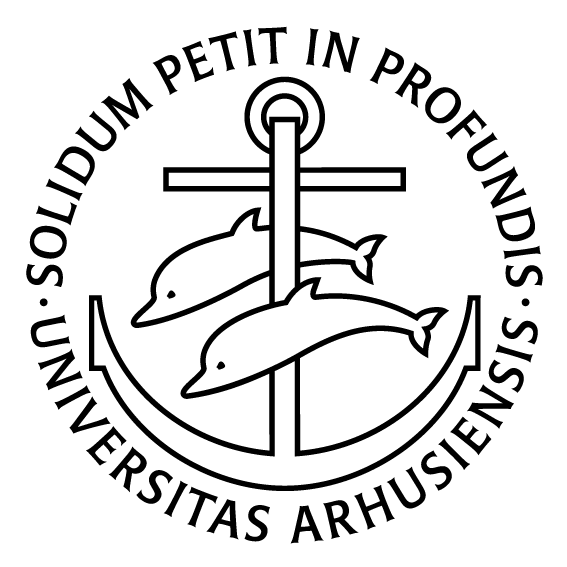
\includegraphics[width=8cm]{ausegl_sort.png}\par
			\vspace*{4\onelineskip}%
			Bachelor Project in Computer Science\par
			Danny Nygård Hansen~~{\footnotesize\textbullet}~~201605113\par
		}%
		\vfill
		\vspace*{2\onelineskip}
		Supervisor: Lars Birkedal\hfill
		10th June 2024\par
		\vspace*{2\onelineskip}%
		\small%
		Department of Computer Science\par
		Aarhus University\par~\par
		%\emph{Må gerne offentliggøres}%
		\enlargethispage{2\onelineskip}
		% \end{adjustwidth}
	\end{adjustwidth}
	\newpage
	%
	% Colophon
    \thispagestyle{empty}
    \small%
    \strut\vfill
    \begin{adjustwidth}{-5cm}{0cm}
        \begin{flushleft}
            Copyright \copyright\ Danny Nygård Hansen 2024

            \plainbreak{1}

            Layout and typography by the author \par
            Font: 10\,pt KP Serif | 8.5\,pt \textsf{Bera Sans} | 8.5\,pt \texttt{Bera Mono} \par
            Typeset using \textsc{pdf}\LaTeX{} and the \classfont{memoir} class \par
            All figures generated using \TikZ

            \plainbreak{1}

            Used packages:
            %
            \begin{multicols}{4}
                \sffamily
                \raggedcolumns
                \begin{itemize}[label={}]
                    % \item adforn
                    \item array
                    \item babel
                    \item beramono
                    \item berasans
                    \item biblatex
                    % \item biolinum
                    \item caption
                    % \item changepage % for sanscolour
                    \item cleveref
                    \item csquotes
                    \item enumitem
                    % \item eufrak
                    % \item FiraMono
                    \item fontenc
                    % \item geometry % for sanscolour
                    \item graphicx
                    \item hyperref
                    \item imakeidx
                    % \item inconsolata
                    \item inputenc
                    \item kpfonts
                    % \item listings
                    % \item longtable
                    \item mathpartir
                    \item mathtools
                    \item microtype
                    \item multicol
                    \item ntheorem
                    \item pgffor
                    % \item subcaption
                    % \item tcolorbox % for sanscolour
                    \item tikz
                    \item tikz-cd
                    \item xcolor
                \end{itemize}
            \end{multicols}
            %
            The source code for this project is available on \href{https://github.com/dnhansen/cs-bachelor-project}{GitHub}.
        \end{flushleft}
    \end{adjustwidth}
    \newpage
\end{titlingpage*}
}









\newcommand{\langrecref}{\ensuremath{\mathbf{F}_{\exists,\mu,\mathrm{ref}}}}
\newcommand{\langpure}{\ensuremath{\mathbf{F}}}




\begin{document}

\frontmatter

% \begin{titlingpage}
%     \calccentering{\unitlength}
%     \begin{adjustwidth*}{\unitlength}{-\unitlength}
%     \maketitle
%     \end{adjustwidth*}
%     \end{titlingpage}
\maketitle

\begin{otherlanguage}{danish}
    \begin{abstract}
        \noindent I denne opgave studerer vi typesikkerhed af en udgave af System $\mathbf{F}$ med referencer og rekursive funktioner og typer. Vi tager først den klassiske tilgang, idet vi beviser sætninger om progress og preservation som medfører typesikkerhed for dette sprog.

        For et fragment af dette sprog uden referencer og rekursion beviser vi også typesikkerhed ved hjælp af et logisk prædikat, og vi definerer en binær logisk relation som kan benyttes til at vise kontekstuel ækvivalens af programmer.
    \end{abstract}
    \end{otherlanguage}
    \begin{abstract}
        \noindent In this report we study type safety of a version of System $\mathbf{F}$ with references and recursive functions and types. We first take the classical approach, proving progress and preservation theorems which imply type safety for this language.

        For a fragment of this language without references and recursion we also prove type safety using a logical predicate, and we define a binary logical relation which can be used to show contextual equivalence of programs.
    \end{abstract}
    
    \cleardoublepage
    
    \tableofcontents
    \cleardoublepage

\chapter{Preface}

For the computer scientist, programming languages and programming in general are both an important tool and an interesting and fruitful subject of study. While we will briefly discuss practical applications of type systems, this report is chiefly concerned with the latter: In particular, we study how to describe programming languages and their semantics in a manner that is amenable to proof, how type systems give guarantees on runtime safety of programs, and how we can talk about two programs being \enquote{the same}.

The genesis of this project was a project course on logical relations led by Lars Birkedal and Simon Oddershede Gregersen in the autumn of 2023, the purpose of my own project essentially being to write up the solutions to exercises in all their gory detail, for the benefit of current and future students. While this purpose can hardly be said to have survived the writing process, I have tried as far as possible to be clear and pedagogical, with the hope that the present report reads more like a textbook than a journal article.

There is of course another motivation for writing a report like this one: Namely, obtaining a bachelor's degree. And the report must then, in part, show that I have learnt enough to warrant this distinction. Hopefully this is the case, though I will certainly claim that the process of writing it has been a great learning experience.

The end result is a report that is, quite frankly, all over the place. I have been rather (some would say too) detailed in my presentation of the syntax and semantics of programming languages, something which I have rarely, if at all, seen done in the introductory literature. On the other hand I make liberal (some would say gratuitous) references to category theory, topology, algebra and even measure theory to try to explicate the concepts being studied. I hope that the reader not familiar with these topics will forgive me.


\section*{Organisation}

\Cref{chap:preliminaries} is a miscellany of foundational topics that appear throughout the report. It covers the elementary theory of inference rules, induction and recursive definitions, making ample use of \cref{app:order-theory} on order theory. Next abstract syntax is introduced, and we give a rather thorough, if informal, treatment of abstract syntax trees in the style of \textcite{harper-pl}. Then follows short sections on reduction, partitions and coinduction, whose purpose is more or less to introduce definitions and fix notation.

In \cref{chap:language-fundamentals} we introduce the two languages we study throughout the rest of the report. These are the pure language \langpure{} which is a variant of Girard's System $\mathbf{F}$, and the extension \langrecref{} which among other things include references as well as recursive functions and types. After a tour of the type system of these languages, we prove some of their fundamental properties. Keywords are \enquote{inversion} and \enquote{canonical forms}.

\Cref{chap:progress-preservation,chap:logical-predicates} are both concerned with type safety. The first of these chapters proves type safety for \langrecref{} using the classic approach of \enquote{progress and preservation}. The second instead focuses on \langpure{} and uses a logical predicate to prove type safety.

Next, \cref{chap:logical-relations} introduces (binary) logical relations, which are extensions of logical predicates to two arguments. We consider how to define equivalence of programs, and define a logical relation as a tool to prove equivalence of concrete programs.

\Cref{app:order-theory} is a fairly extensive and mostly self-contained appendix covering elementary order theory with a view towards the fixed-point theorems we need to get us off the ground in \cref{chap:preliminaries}. We generalise the theory beyond what is necessary for our purposes: It turns out that the theory underlying recursive definitions of things like type systems or operational semantics appears in a more general context in mathematics, in particular in topology and measure theory. While a more elementary approach is sufficient to cover our applications of the theory, we wish to highlight exactly what it is that makes type systems different from e.g. topologies or $\sigma$-algebras. This all but necessitates the use of transfinite induction and recursion, but we provide an elementary path through the material for readers either not familiar with the requisite set theory, or readers simply not interested in the aforementioned generalisations.

\Cref{app:syntax-semantics} collects the syntax and semantics of our languages. To avoid cluttering the body of the text, this is the only place the complete specifications of the languages are located. To mitigate flipping to and from this appendix, we thus encourage the reader to either open a second copy of this report in another window, or to use a pdf-reader with a \enquote{back}-button. Every cross reference includes a link for precisely this purpose.

Finally, after the bibliography are located two fairly extensive indices that will hopefully help the reader find their way through the report.


\section*{Acknowledgments}

I am first and foremost greatly indebted to my supervisor Lars Birkedal, and I thank him for his guidance and generosity throughout the project. Thanks are also due to Simon Oddershede Gregersen for his guidance on the logical relations project, to Amin Timany for preparing the initial specification of the languages studied in the project, and to Lau Skorstengaard without whose notes on logical relations there might not have been a project in the first place. Finally I thank Gerth Stølting Brodal and Asger Klinkby Jørgensen for inadvertently inspiring me to study computer science.

\enlargethispage{2\onelineskip}

\vspace{\baselineskip}

\noindent Aarhus, June 2024 \hfill Danny Nygård Hansen


\mainmatter

\chapter{Preliminaries}\label{chap:preliminaries}

This first chapter introduces various topics that will be needed in the sequel. In particular we consider recursive definitions of sets and functions, inference rules and generating functions, abstract syntax, reduction systems, partitions and coinduction.

\section{Notation}

We begin by fixing notation.

If $X$ is a set, then we denote by $\powerset{X}$\index[notation]{pz-PX@$\powerset{X}$} the power set of $X$, and for a cardinal $\kappa$\blfootnote{Readers unfamiliar with cardinal and ordinal numbers can for our purposes safely think of $\kappa$ as an element of $\naturals \union \{\infty\}$, and of $\omega$ as $\infty$.} we furthermore write $\powersetcard{\kappa}{X}$\index[notation]{pz-PXk@$\powersetcard{\kappa}{X}$} for the collection of subsets of $X$ with cardinality strictly less than $\kappa$. If $A \in \powersetcard{\kappa}{X}$, then we also write $A \subseteq_\kappa X$\index[notation]{***-subseteqk@$\subseteq_\kappa$}. For ordinals $\alpha$ we do not distinguish between the ordinal $\omega_\alpha$\index[notation]{ozz-omegaalpha@$\omega_\alpha$} and the cardinal $\aleph_\alpha$\index[notation]{azzzzz-alephalpha@$\aleph_\alpha$}, and we write $\omega \defeq \omega_0$\index[notation]{ozz-omega@$\omega$}\index[notation]{ozz-omega0@$\omega_0$}. Hence $\powersetfin{X}$\index[notation]{pz-PXo@$\powersetfin{X}$} denotes the set of finite subsets of $X$, and $A \subseteq_\omega X$\index[notation]{***-subseteqomega@$\subseteq_\omega$} means that $A$ is a finite subset of $X$.

If $Y$ is another set, then we denote the set of partial maps from $X$ to $Y$ by $\pmaps{X}{Y}$\index[notation]{xz-XY@$\pmaps{X}{Y}$}. If $f \in \pmaps{X}{Y}$ then we let $\dom f$\index[notation]{dom@$\dom$} and $\ran f$\index[notation]{ran@$\ran$} denote the domain and range of $f$, respectively. We also write $\pmaps[\kappa]{X}{Y}$\index[notation]{xz-XYkappa@$\pmaps[\kappa]{X}{Y}$} for the partial functions $f \in \pmaps{X}{Y}$ with $\dom f \subseteq_\kappa X$. For $x_0 \in X$ and $y_0 \in Y$ we denote by $f[x_0 \mapsto y_0]$\index[notation]{f-fxy@$f[x_0 \mapsto y_0]$} the partial map given by
%
\begin{equation*}
    f[x_0 \mapsto y_0](x) =
    \begin{cases}
        y_0, & x = x_0, \\
        f(x), & x \in \dom f \setminus \{x_0\}.
    \end{cases}
\end{equation*}
%
Hence $\dom f[x_0 \mapsto y_0] = \dom f \union \{x_0\}$, so that if $f \in \pmapsfin{X}{Y}$, then also $f[x_0 \mapsto y_0] \in \pmapsfin{X}{Y}$. Any partial map with empty domain is denoted $\bot$.

We let $\naturals$\index[notation]{nzzz-N@$\naturals$} denote the set of natural numbers, including $0$, $\ints$\index[notation]{zzzz-Z@$\ints$} the set of integers, and $\posints$\index[notation]{nzzz-Nplus@$\posints$} the set of strictly positive integers.

The image of a set $A \subseteq X$ under a function $f \colon X \to Y$ is denoted $f\image{A}$.\index[notation]{f-fA@$f\image{A}$}\blfootnote{It is common to write simply $f(A)$ for the image of $A$ under $f$, relying on context to distinguish this from the value of $f$ at an \emph{element} $A$ of $X$.} We similarly write $f\preim{B}$\index[notation]{f-fB@$f\preim{B}$} for the preimage of $B \subseteq Y$ under $f$. The restriction of $f$ to $A$ is denoted $f|_A$\index[notation]{f-frestrictA@${f|_A}$}.

An \keyword{indexed family}\index[subject]{indexed family} of elements of a set $X$ is a map $I \to X$, where $I$ is any set called the \keyword{index set}\index[subject]{index set} of the family. If $\calA$ is an indexed family of elements of $X$ and $Y$ is some set, then we write $\calA \subseteq Y$ if the image of $\calA$ is a subset of $Y$. If the image of $i \in I$ under the indexed family is $x_i$, then we also write $(x_i)_{i \in I}$.\index[notation]{x-xiiI@$(x_i)_{i \in I}$} If $I$ is the finite set $\{1,\ldots,n\}$, then we also denote the family $(x_i)_{i \in I}$ by $\seq{x}$\index[notation]{x-xseq@$\seq{x}$}. The set of finite sequences of elements from $X$ is denoted $X^*$\index[notation]{xz-Xstar@$X^*$}.

\clearpage
\section{Definition by recursion}

\subsection{Generating functions}

Let $(P,\leq)$ be a poset, and let $f \colon P \to P$ be a monotone map. We think of $f$ as a \keyword{generating function}\index[subject]{generating function}, in the sense that given an element $x \in P$ representing a set of states of some system, it generates a new set of states $f(x)$. The fact that $f$ is monotone models that given a larger set of states as input, a larger set of new states is also generated.

We wish to find an element $x \in P$ such that $f$ cannot generate anything new from it \textdash i.e., $x$ should be $f$-closed \textdash and we don't want this element to contain any \enquote{redundancies}: It should contain only those states mandated by $f$. More precisely, $x$ should be the \emph{least} $f$-closed element in $P$. But \cref{lem:least-closed-implies-fixed-point} says that $x$ is then a fixed-point of $f$, indeed its smallest fixed-point, and is denoted $\lfp{f}$. Hence we may instead focus our attention on fixed-points.

In this generality it is not possible to systematically study the fixed-points of $f$. Indeed, $f$ may not even have any! Hence we must impose appropriate further requirements on $P$ or $f$. If $P$ is a power set, then it is in particular a complete lattice, and we thus have access to the Knaster--Tarski fixed-point theorem (cf. \cref{thm:knaster-tarski}), ensuring the existence of both a least and a greatest fixed-point.

We will also have occasion to consider fixed-points of monotone functions defined on posets that are not complete lattices. Most importantly, notice that a set $\pmaps{X}{Y}$ of partial functions is not generally a complete lattice, but that it does satisfy a collection of weaker properties:\marginbox{Reminder}{A subset $D$ of a poset $P$ is directed if every finite subset of $D$ has an upper bound in $D$.} The empty map $\bot$ is its least element, and every directed subset $D$ of $\pmaps{X}{Y}$ has a join, namely the map whose graph is the union of the graphs of the elements in $D$. This means that $\pmaps{X}{Y}$ is a \dCPPO{}, and thus Kleene's fixed-point theorem applies (cf. \cref{thm:Kleene-I,thm:Kleene-II}). This also ensures that $\lfp{f}$ is the least $f$-closed element of $P$. Especially important in the present context is the following:

\begin{corollarynoproof}[Principle of induction]
    \label{cor:induction-abstract}\index[subject]{induction}
    Let $P$ be a \dCPPO{} and let $f \colon P \to P$ be monotone. If $y \in P$ is $f$-closed, then $\lfp{f} \leq y$.
\end{corollarynoproof}


\subsection{Inference rules}\label{sec:inference-rules}

Specialising\blfootnote{When we in \cref{thm:recursive-definitions} study how to define functions recursively using inference rules, it will be important that $H$ is indexed. Compare e.g. \textcite[§7.1]{pitts-nominal-sets} who only considers $H$ as a set.} to the case where $P$ is a power set $\powerset{X}$, one way to define a generating function is using inference rules. An \keyword{inference rule}\index[subject]{inference rule} over $X$ is a pair $(H,y)$, where $H$ is an indexed family of elements of $X$ called the \keyword{hypotheses}\index[subject]{inference rule!hypothesis} of the rule, and $y \in X$ is its \keyword{conclusion}\index[subject]{inference rule!conclusion}. We denote this rule by\footnote{This is not standard notation. \textcite[§7.1]{pitts-nominal-sets} simply denotes it by $(H,y)$, but we prefer to use a slightly more distinctive notation.} $\myinfrule{}{H}{y}$\index[notation]{***-inference@$\myinfrule{}{}{}$}, and if we give this rule the name $R$, then we also write $\myinfrule{R}{H}{y}$. The index set of $H$ is then also denoted $\idxset{R}$\index[notation]{izzzz-iR@$\idxset{R}$}.

If $R$ has finitely many premises $\seq{x} = (x_1, \ldots, x_n)$, then we say that $R$ is \keyword{finitary}\index[subject]{inference rule!finitary}. In this case we naturally write $\myinfrule{R}{\seq{x}}{y}$, and we also use the notation
%
\begin{equation*}
    \inferrule*[lab={$R$}, right={.}]{
        x_1 \and x_2 \and \cdots \and x_n
    }{
        y
    }
\end{equation*}
%
We allow $n$ to be zero, in which case we call the rule an \keyword{axiom}\index[subject]{axiom}\index[subject]{inference rule!axiom} and write $\myinfrule{}{}{y}$.

Given a (usually infinite)\blfootnote{While the collection of inference rules will usually be infinite, they will be presented in the form of finitely many rule \emph{schemas}, as is usual when presenting axioms in (first-order) logic.} collection $\calR$ of inference rules, we construct a generating function $F \colon \powerset{X} \to \powerset{X}$ by defining $F(A)$ for a subset $A \subseteq X$ as follows: For $y \in X$ we let $y \in F(A)$ if and only if there is a rule $\myinfrule{}{H}{y}$ in $\calR$ with $H \subseteq A$. We say that $F$ is \keyword{represented by}\index[subject]{inference rule!represented by} $\calR$. In this case $F$ is clearly monotone, so by \cref{thm:knaster-tarski} it has a least and a greatest fixed-point. Since it is often unnecessary to explicitly talk about $F$, we also write $\lfp{\calR}$\index[notation]{mzzzz-muR@$\lfp{\calR}$} and $\gfp{\calR}$\index[notation]{nzzzz-nuR@$\gfp{\calR}$} for these fixed-points.

By \cref{cor:induction-abstract} we also get a principle of induction for $F$. However, it is useful to restate induction in terms of the inference rules, since we usually have explicit rules in mind when defining $F$. If $\calR$ is a collection of inference rules on $X$, then we say that a subset $K \subseteq X$ is \keyword{$\calR$-closed}\index[subject]{R-closed@$\calR$-closed} if, given any rule $\myinfrule{}{A}{y}$ in $\calR$, $A \subseteq K$ implies that $y \in K$.

\begin{lemma}
    \label{lem:R-closed-F-closed}
    If $F$ is represented by a collection $\calR$ of inference rules, then a subset $A \subseteq X$ is $F$-closed if and only if it is $\calR$-closed.
\end{lemma}

\begin{proof}
    First assume that $A$ is $F$-closed so that $F(A) \subseteq A$, and consider a rule $\myinfrule{}{H}{y}$ from $\calR$ with $H \subseteq A$. Since $F$ is represented by $\calR$, this implies that $y \in F(A) \subseteq A$, so $A$ is $\calR$-closed.

    If $A$ is $\calR$-closed, then let $y \in F(A)$. Then there is a rule $\myinfrule{}{H}{y}$ in $\calR$ with $H \subseteq A$. But since $A$ is $\calR$-closed, this implies that $y \in A$, and so $F(A) \subseteq A$.
\end{proof}

\begin{theorem}[Principle of rule induction]
    \label{thm:rule-induction}\index[subject]{rule induction}\index[subject]{induction!rule}
    If $\calR$ is a set of inference rules on $X$ and $A \subseteq X$, then $\lfp{\calR} \subseteq A$ if and only if the following condition holds: For every inference rule $\myinfrule{}{H}{y}$ in $\calR$, $H \subseteq A$ implies $y \in A$.
\end{theorem}

\begin{proof}
    Let $F$ be the function represented by $\calR$. The condition says precisely that $A$ is $\calR$-closed, which by \cref{lem:R-closed-F-closed} is equivalent to $A$ being $F$-closed. The claim thus follows from \cref{cor:induction-abstract}.
\end{proof}

\marginbox{Reminder}{An element $A \in \powerset{X}$ is $F$-consistent if $A \subseteq F(A)$, cf. \cref{enum:consistent-element-definition}.} Notice that the principle of induction follows since fixed-points are closed. But fixed-points are also \emph{consistent}, which leads to the following important result:

\begin{theorem}[Inversion]
    \label{thm:inversion}\index[subject]{inversion!inference rules}
    If $\calR$ is a collection of inference rules and $y \in \lfp{\calR}$, then there is a rule $\myinfrule{}{H}{y}$ in $\calR$ such that $H \subseteq \lfp{\calR}$.
\end{theorem}

\begin{proof}
    Let $F$ be the function represented by $\calR$. Then we in particular have $y \in \lfp{F} \subseteq F(\lfp{F})$, which by definition of $F$ implies that there is an inference rule $\myinfrule{}{H}{y}$ with $H \subseteq \lfp{F}$, as desired.
\end{proof}
%
This is particularly useful if there to any $y \in \lfp{\calR}$ is a \emph{unique} inference rule with $y$ as its conclusion, but sometimes this is not even necessary, as long as we have the right knowledge about which inference rules have $y$ as their conclusion. We will see an application of this in \cref{lem:inversion-typing}.

These kinds of results are sometimes proved by rule induction, for instance by \textcite[§7.2]{pitts-nominal-sets} or \textcite[Lemma~4.2]{harper-pl}, and this approach is indeed more elementary, circumventing \cref{thm:knaster-tarski} or similar results. But notice that the proof above does not have anything to do with induction: Indeed, as mentioned above induction concerns properties of \emph{closed} sets, while inversion follows from the \emph{consistency} of fixed-points. In fact, the proof of \cref{thm:inversion} goes through if $\lfp{\calR}$ is replaced with any $F$-consistent set.

Inversion is also sometimes justified by appealing to a notion of \enquote{derivation} of elements of $\lfp{\calR}$, by arguing that $y$ is obtained by applying a series of inference rules to the set of axioms. It is then claimed that there is a \emph{last} such application, which must have the form $\myinfrule{}{H}{y}$, and since this application is valid it follows that $H \subseteq \lfp{\calR}$. If all rules in $\calR$ are finitary, then it is indeed possible, and in fact very simple, to set up a deductive calculus that does precisely this. This is the approach taken in \textcite[e.g. Remark~2A8.6]{hindley-type-theory}, using a version of natural deduction.


\subsection{Recursive functions}

As is usual, the above principle of proof by induction allows us to define functions by recursion.


\subsubsection{Total functions}

We begin by proving that we can define total functions recursively. In contrast to recursion on $\naturals$, it may be possible to obtain an element of the relation $\lfp{\calR}$ by applying multiple different rules, in which case it is not obvious that a purported recursive function is well-defined. We only consider the case where each element in $\lfp{\calR}$ is the conclusion of a unique rule, since this is all we will need in the sequel.

\begin{theorem}[Recursion]
    \label{thm:recursive-definitions}\index[subject]{recursion}\blfootnote{The statement of \cref{thm:recursive-definitions} is based on \textcite[Corollary~5.12]{moschovakis-set-theory}, while the proof is inspired by \textcite[§8.18]{davey-priestley-order} and \textcite[§6.30]{moschovakis-set-theory}.}
    Let $\calR$ be a set of inference rules such that each $y \in \lfp{\calR}$ is the conclusion of a unique rule, and let $Z$ be any set. For each $R \in \calR$ let $h_R \colon \lfp{\calR} \prod Z^{\idxset{R}} \to Z$ be a function. Then there is a unique function $f \colon \lfp{\calR} \to Z$ such that if $\myinfrule{R}{(x_i)_{i \in \idxset{R}}}{y}$, then
    %
    \begin{equation}
        \label{eq:recursion-fixed-point-equation}
        f(y)
            = h_R \bigl( y, (f(x_i))_{i \in \idxset{R}} \bigr).
    \end{equation}
\end{theorem}

\begin{proof}
    Define a function $G \colon \pmaps{\lfp{\calR}}{Z} \to \pmaps{\lfp{\calR}}{Z}$ as follows: For $f \colon \lfp{\calR} \pto Z$ let $\dom G(f)$ be the set of elements $y \in \lfp{\calR}$ such that if $\myinfrule{R}{(x_i)_{i \in \idxset{R}}}{y}$ is the unique rule with conclusion $y$, then $(x_i)_{i \in \idxset{R}} \subseteq \dom f$. For $y \in \dom G(f)$ we then let
    %
    \begin{equation*}
        G(f)(y)
            = h_R \bigl( y, (f(x_i))_{i \in \idxset{R}} \bigr).
    \end{equation*}
    %
    Clearly $G$ is monotone, so \cref{thm:Kleene-II} implies that $G$ has a least fixed-point $f^*$.

    We prove that $f^*$ is indeed a total function, i.e., that $\lfp{\calR} \subseteq \dom f^*$. By \cref{thm:rule-induction} it suffices to show that if $\myinfrule{R}{(x_i)_{i \in \idxset{R}}}{y}$ is a rule with $(x_i) \subseteq \dom f^*$, then also $y \in \dom f^*$. But notice that $\dom f^* = \dom G(f^*)$, so $y$ lies in $\dom f^*$ just when $(x_i) \subseteq \dom f^*$. Hence $f^*$ is total. It follows that
    %
    \begin{equation*}
        f^*(y)
            = G(f^*)(y)
            = h_R \bigl( y, (f^*(x_i))_{i \in \idxset{R}} \bigr)
    \end{equation*}
    %
    for all rules $\myinfrule{R}{(x_i)_{i \in \idxset{R}}}{y}$.

    Finally, to prove that $f^*$ is unique simply note that any partial function $f$ that satisfies \cref{eq:recursion-fixed-point-equation} is a fixed-point of $G$, so $f^* \leq f$ by minimality of $f^*$. But since $f^*$ is total, this implies that $f^* = f$.
\end{proof}



\subsubsection{Finitary rules}

If every rule in $\calR$ is finitary, then it turns out that we can avoid an appeal to \cref{thm:Kleene-II}, instead using \cref{thm:Kleene-I}. Of course $G$ is monotone, and we claim that it is compact (cf.~\cref{def:compact-map}). Assume that $f \in \dom G$ and $y \in \dom G(f)$. If $\myinfrule{}{\seq{x}}{y}$ is the unique rule with $y$ as conclusion, let $f_0 \defeq f|_{\seq{x}}$. Then $f_0$ is finite and $y \in \dom G(f_0)$ with
%
\begin{align*}
    G(f_0)(y)
        &= h_R \bigl( y, f_0(x_1), \ldots, f_0(x_n) \bigr) \\
        &= h_R \bigl( y, f(x_1), \ldots, f(x_n) \bigr) \\
        &= G(f)(y),
\end{align*}
%
so $G$ is compact. Hence it is continuous by \cref{prop:partial-map-continuity-equivalent}, so \cref{thm:Kleene-I} implies that $G$ has a least fixed-point $f^*$. The rest of the proof is identical to the above.


\subsubsection{Partial functions}

We also sometimes wish to define \emph{partial} functions recursively. This is no issue due to the correspondence between partial and total functions described in \cref{sec:pmaps-topology}: To define a partial function $f \colon X \pto Y$, first define a total function $f_* \colon X \to Y_*$ by recursion, letting $f_*(x) = *$ if $x$ is supposed to lie outside the domain of $f$. Then restrict $f_*$ to the set $\set{x \in X}{f_*(x) \neq *}$.

\section{Abstract syntax}

In this report we have no interest in the concrete syntax of languages; instead we seek an abstract representation of the structure of programs. We describe one formulation of abstract syntax trees \textdash inspired by \textcite{harper-pl} \textdash but we do not go into painstaking detail in either the definition of such trees, nor in the proofs of their properties, for a few reasons:
%
\begin{itemize}
    \item The definition of abstract syntax trees that support bindings (what \citeauthor{harper-pl} calls \enquote{abstract binding trees}\index[subject]{abstract binding tree}) is fairly involved, and our naïve understanding of abstract syntax is accurate enough not to cause issues.

    \item What is important is not the precise formulation of any kind of abstract syntax, but rather its existence and basic properties.
    
    \item An abstract syntax that is readable to humans is difficult to formalise in a proof assistant, so if that is our ultimate goal then we will have to revisit these issues anyway.
\end{itemize}
%
While our abstract syntax is of course heavily inspired by the $\lambda$-calculus, note that the $\lambda$-calculus is usually defined\footnote{For instance by \textcite{barendregt-lambda}.} by a \emph{concrete} syntax (i.e., as a formal language).


\subsection{Abstract syntax trees}

An \keyword{abstract syntax tree}\index[subject]{abstract syntax tree} (or simply \keyword{AST}\index[subject]{AST|see{abstract syntax tree}}) is a rooted tree whose leaves are variables, and whose interior nodes are operators. Operators simultaneously play the roles of functions and of binding constructs, analogous to function symbols and quantifiers in formal logic, respectively. Therefore, each operator not only has an arity (which may be zero), for each argument it also specifies which variables it binds inside this argument.

We may use inference rules to define the set of ASTs. Fix some infinite set $\setVarAST$ of variables\blfootnote{Since programs are finite, $\setVarAST$ need not be more than countably infinite, but for our purposes we do not need to assume that it is countable.}\index[subject]{variable!in ASTs} and $\setOp$ of operators\index[subject]{operator} which have been assigned arities\index[subject]{operator!arity}. For each $x \in \setVarAST$ we have the axiom
%
\begin{equation}
    \label{eq:AST-var}
    \inferrule{ }{
        \phantom{x}x\phantom{x}
    }
\end{equation}
%
saying that $x$ itself is an AST. Next, say that the operator $\phi \in \setOp$ takes $n$ arguments, and in the $i$th argument it binds $k_i$ variables. If $a_1, \ldots, a_n$ are ASTs and $\seq{x}_i \in \setVarAST^{k_i}$, then we have the rule\blfootnote{For instance, we might have an AST on the form $\textsf{let}(a;x.b)$, which has the desired interpretation of letting $x \defeq a$ in $b$. Since there are no variables bound in the first argument, we have omitted the period.}
%
\begin{equation}
    \label{eq:AST-op}
    \inferrule{
        a_1 \and \cdots \and a_n
    }{
        \phi(\seq{x}_1.a_1 ; \ldots ; \seq{x}_n.a_n) \index[notation]{pzzzz-phhix1a1@$\phi(\seq{x}_1.a_1 ; \ldots ; \seq{x}_n.a_n)$} % TODO doesn't work without bm, with bm it's computer modern??
    }
\end{equation}
%
This is supposed to denote the application of the operator $\phi$ to the ASTs $a_1, \ldots, a_n$, in which the variables $\seq{x}_1, \ldots, \seq{x}_n$ have been bound, yielding a new AST. It should be clear that any AST is the conclusion of a unique rule; on the other hand, many rules with the same hypotheses have different conclusions.

Of course, for this to be well-defined we need some \enquote{ground set} from which we draw the ASTs, i.e., which plays the role of the set $X$ in \cref{sec:inference-rules}. We do not care precisely what $X$ looks like, but if we think of expressions such as $\phi(\seq{x}_1.a_1 ; \ldots ; \seq{x}_n.a_n)$ as being a sort of nested tuple, then we can take $X$ to be the set of all finitely nested tuples whose elements are operators or variables.\blfootnote{We do not wish to think of expressions such as $\phi(\seq{x}_1.a_1 ; \ldots ; \seq{x}_n.a_n)$ as denoting \emph{formal} expressions, as this would defeat the purpose of defining an \emph{abstract} syntax, requiring us to concern ourselves with issues of parsing, unique readability, etc.}

\begin{definition}[Abstract syntax trees]
    The set of \keyword{abstract syntax trees}\index[subject]{abstract syntax tree} with variables $\setVarAST$ and operators $\setOp$ is the set generated by the inference rules \cref{eq:AST-var} and \cref{eq:AST-op} and is denoted $\setAST{\setVarAST}{\setOp}$\index[notation]{azzz-aVO@$\setAST{\setVarAST}{\setOp}$}.
\end{definition}


\subsubsection{Free and bound variables}

Having defined the set of ASTs recursively, \cref{thm:recursive-definitions} allows us to recursively define functions on ASTs: We first define what is meant by \keyword{free variables}\index[subject]{free variable}\index[subject]{variable!free}. This will be a function $\freevar{} \colon \setAST{\setVarAST}{\setOp} \to \powerset{\setVarAST}$\index[notation]{fz-FV@$\freevar{}$} with the properties
%
\begin{align*}
    \freevar{x}
        &= \{x\}, \\
    \freevar[\big]{\phi(\seq{x}_1.a_1 ; \ldots ; \seq{x}_n.a_n)}
        &= \bigunion_{i=1}^n \bigl( \freevar{a_i} \setminus \seq{x}_i \bigr).
\end{align*}
%
The function $\freevar{}$ is usually \enquote{defined} simply by writing down the above two equations, but to properly justify this definition we must go through \cref{thm:recursive-definitions}. We illustrate the application of this theorem once, leaving it implicit in later recursive definitions.

According to the theorem, we must specify for each inference rule $R$ a function $h_R \colon \setAST{\setVarAST}{\setOp} \prod \powerset{\setVarAST}^{\idxset{R}} \to \powerset{\setVarAST}$. If $R$ is a rule as in \cref{eq:AST-var}, then $\idxset{R} = \emptyset$ and we let $h_R(a) = \{a\}$. If instead $R$ is as in \cref{eq:AST-op}, then we let\blfootnote{If the first argument to $h_R$ is instead a variable, then we may let the value of $h_R$ be an arbitrary element of $\powerset{\setVarAST}$.}
%
\begin{equation*}
    h_R \bigl( \phi(\seq{x}_1.a_1 ; \ldots ; \seq{x}_n.a_n), A_1, \ldots, A_n \bigr)
        = \bigunion_{i=1}^n (A_i \setminus \seq{x}_i).
\end{equation*}
%
It is then easy to check that \cref{thm:recursive-definitions} yields a function $f = \freevar{}$ with the desired properties.

We similarly define the set of \keyword{bound variables}\index[subject]{bound variable}\index[subject]{variable!bound} in an AST by
%
\begin{align*}
    \boundvar{x}
        &= \emptyset, \\ \index[notation]{bz-BV@$\boundvar{}$}
    \boundvar[\big]{\phi(\seq{x}_1.a_1 ; \ldots ; \seq{x}_n.a_n)}
        &= \bigunion_{i=1}^n \bigl( \seq{x}_i \union \boundvar{a_i} \bigr).
\end{align*}
%
The set of all variables occurring in an AST $a$ is then $\allvar{a} \defeq \freevar{a} \union \boundvar{a}$\index[notation]{vz-V@$\allvar{}$}. If $\freevar{a} = \emptyset$, then we say that $a$ is \keyword{closed}\index[subject]{abstract syntax tree!closed} and otherwise that it is \keyword{open}\index[subject]{abstract syntax tree!open}.


\subsubsection{Sorts}

We wish to be able to construct ASTs which both contains expressions and types, first of all to obtain a unified way of describing these entities syntactically, as well as to support language features such as type annotations\index[subject]{type annotation}, ascription\index[subject]{ascription}, and so on. Expressions and types are examples of \keyword{sorts}\index[subject]{sort}\index[subject]{abstract syntax tree!sort}. We let $\setSort$ be a set of sorts, and we attribute sorts to variables and operators in the following way:\blfootnote{To build the function type $\tau_1 \to \tau_2$ as an AST we might write $\textsf{func}(\tau_1;\tau_2)$. An expression of this type could be the explicitly typed lambda abstraction $\textsf{lam}(\tau_1;x.e)$, which takes as arguments an AST $\tau_1$ of type sort, and an AST $e$ of expression sort in which the parameter $x$ is bound.}
%
\begin{itemize}
    \item Each variable is assigned a sort. The set of variables with sort $s$ is denoted $\setVarAST_s$, and we assume that there are infinitely many variables of each sort.
    \item Each operator $\phi$ of arity $n$, which binds $k_i$ variables in its $i$th argument, is assigned $k_1 + \cdots + k_n + n + 1$ sorts: One for each bound variable, one for each of the $n$ arguments, and one as its \keyword{return sort}\index[subject]{operator!return sort}. We denote this collection of sorts by $\arity{\seq{s}_1.t_1 ; \ldots ; \seq{s}_n.t_n}{s}$\index[notation]{s-s1t1@$\arity{\seq{s}_1.t_1 ; \ldots ; \seq{s}_n.t_n}{s}$} to match the notation for the application of $\phi$ to a series of ASTs. Call this collection of sorts the \keyword{arity}\index[subject]{operator!arity} of $\phi$.
\end{itemize}
%
We leave open the question of whether variables and operators can be assigned multiple sorts and arities at the same time, and return to this in \cref{sec:dynamic-semantics}. Our languages will only have two sorts, expressions and types, but we could also use sorts for various other purposes, for instance to distinguish between pure and impure parts of the language.\footnote{For an example of this, see \textcite[Chapter~34]{harper-pl}.}

We assign sorts to ASTs by defining a binary relation $\hassort{a}{s}$ with $a \in \setAST{\setVarAST}{\setOp}$ and $s \in \setSort$\index[notation]{a-as@$\hassort{a}{s}$} as follows: For $x \in \setVarAST_s$ we have the rule
%
\begin{equation*}
    \inferrule*{ }{
        \hassort{x}{s}
    }
\end{equation*}
%
and for an operator $\phi \in \setOp$ with arity $\arity{\seq{s}_1.t_1; \ldots; \seq{s}_n.t_n}{s}$ we have the rule
%
\begin{equation*}
    \inferrule*{
        \hassort{a_1}{t_1} \and \cdots \and \hassort{a_n}{t_n}
    }{
        \hassort{\phi(\seq{x}_1.a_1; \ldots; \seq{x}_n.a_n)}{s}
    }
\end{equation*}
%
where each $\seq{x}_i \in \finseq{\setVarAST}$ is a sequence of variables with sorts $\seq{s}_i$. Again we need some ground set to define this relation on, but this is simply $\setAST{\setVarAST}{\setOp} \prod \setSort$.

If $s$ is a sort, then we write $\freevarsort{s}{a}$\index[notation]{fz-FVs@$\freevarsort{s}{}$} for the set of free variables in $a$ of sort $s$.


\subsection{\texorpdfstring{$\alpha$}{alpha}-equivalence and substitution}

Properly defining substitution is rather technical and would take us too far afield, so we give an overview of the problems one has to consider to make it precise.


\subsubsection{\texorpdfstring{$\alpha$}{alpha}-equivalence}

Inspired by the $\lambda$-calculus, we say that two ASTs $a,b \in \setAST{\setVarAST}{\setOp}$ are \keyword{$\alpha$-equivalent}\index[subject]{a-equivalence@$\alpha$-equivalence}\index[subject]{abstract syntax tree!$\alpha$-equivalence}, written $a \alphaeq b$\index[notation]{***-alphaeq@$\alphaeq$}, if we may obtain $b$ from $a$ by renaming bound variables. Some care must be taken in that not all renamings are allowed\footnote{For instance, if an operator $\phi$ binds two variables $x$ and $y$ in the same argument, say $\phi(xy.a)$, we clearly do not allow $x$ to be renamed $y$, or vice versa. If $a$ already contains another free variable $z$, then we also do not allow $x$ to be renamed $z$.}, but we won't go into detail. It is clear that $\alphaeq$ is an equivalence relation. Furthermore, one can show that renaming respects sorts in the sense that if $\hassort{a}{s}$ and $x$ and $y$ are variables of the same sort, then renaming $x$ to $y$ in $a$ yields an AST of sort $s$.

It is standard to use the so-called \keyword{Barendregt convention}\index[subject]{Barendregt convention}\footnote{See \textcite[\nopp 2.1.13]{barendregt-lambda}, though he of course did not name it after himself, instead calling it the \enquote{variable convention}\index[subject]{variable convention}.}: This says that whenever ASTs $a_1, \ldots, a_n$ occur in the same context, we choose the bound variables in each $a_i$ such that the sets $\freevar{a_1} \union \cdots \union \freevar{a_n}$ and $\boundvar{a_1} \union \cdots \union \boundvar{a_n}$ are disjoint. In our setting we must also choose the new bound variables to have the same sorts as the original ones. This is clearly possible since we have infinitely many variables of each sort, and we need only perform finitely many renamings.

There are also other ways of dealing with bound variables, most notably \keyword{de Bruijn indices}\index[subject]{de Bruijn indices} (see for instance \cite[Appendix~C]{barendregt-lambda}). These are less human-friendly but are more amenable to formalisation.


\subsubsection{Substitution}\index[subject]{abstract syntax tree!substitution}

Defining substitution is tricky, not least because of its relationship with $\alpha$-equivalence. We take the following approach: If $a$ and $b$ are ASTs, then we roughly speaking define $a[b/x]$ to be the AST\footnote{The precise definition of substitution makes it clear that $a[b/x]$\index[notation]{a-abx@$a[b/x]$} is in fact an AST.} obtained by replacing every occurrence of $x$ in $a$ with $b$, if this is allowed. Some such substitutions will be undefined\footnote{As an example, if $x \neq y$, $x$ is free in $a$ and $y$ is free in $b$, then the substitution $\phi(y.a)[b/x]$ is undefined, since the free occurrences of $y$ in $b$ would be \enquote{captured} by the binding of $y$.}, but one can show that it is always possible to find an AST $a'$ with the same sort as $a$, such that $a \alphaeq a'$ and $a'[b/x]$ is defined.

It then turns out that substitution preserves $\alpha$-equivalence, in the sense that if $a \alphaeq a'$ then $a[b/x] \alphaeq a'[b/x]$, as long as the substitutions are defined. Hence we may define substitution on $\alpha$-equivalence classes by
%
\begin{equation*}
    [a]_\alpha [b/x]
        \defeq \bigl[ a[b/x] \bigr]_\alpha,
\end{equation*}
%
where $[a]_\alpha$ is the $\alpha$-equivalence class of $a$, and where we choose the representative $a$ such that $a[b/x]$ is defined.

Furthermore, it is of course possible to follow the Barendregt convention while choosing $\alpha$-equivalent ASTs to perform substitution.


\section{Reduction}

\subsection{Abstract reduction systems}

An \keyword{abstract reduction system}\index[subject]{abstract reduction system}\blfootnote{An abstract reduction system is also called an abstract \emph{rewriting} system\index[subject]{abstract rewriting system} to underline the fact that the reduction $\to$ may not in fact describe a \enquote{reduction} in the usual sense of the word.} is a pair $(X,\to)$, where $X$ is a set and $\to$ is a binary relation on $X$ called a \keyword{reduction}\index[subject]{reduction}.\blfootnote{Recall that a (binary) relation between sets $X$ and $Y$ is simply a subset $R \subseteq X \prod Y$. If $(x,y) \in R$, then we also write $xRy$\index[notation]{xRy@$xRy$}. If $S \subseteq Y \prod Z$ is another relation, recall the composition\index[subject]{composition!of binary relations} $S \circ R \subseteq X \prod Z$\index[notation]{****-circ@$\circ$ (composition of relations)}: Writing $R \cdot S \defeq S \circ R$\index[notation]{****-@$\cdot$ (composition of relations)} following \textcite[Definition~A.1.1(iii)]{terese-rewriting}, this is defined so that $x(R \cdot S)z$ if and only if $xRy$ and $ySz$ for some $y \in Y$. If $X = Y$, then we write $R^n$\index[notation]{rz-Rn@$R^n$} for the $n$-fold composition $R \circ \cdots \circ R$ and $R^*$\index[notation]{rz-Rstar@$R^*$} for the reflexive\index[subject]{reflexive closure} and transitive closure\index[subject]{transitive closure} $\bigunion_{n \in \naturals} R^n$, where $R^0$ by definition is equality. The reflexive and transitive closure of a relation $\to$ is also often denoted $\twoheadrightarrow$\index[notation]{***-arr2head@$\twoheadrightarrow$}. Finally, the inverse\index[subject]{inverse!of binary relation} $R\inv$\index[notation]{rz-Rinv@$R\inv$} of the relation $R$ is defined by the property that $xR\inv y$ if and only if $yRx$.} In the present context, $X$ will be a set of expressions in a language, and $\to$ will describe how expressions may reduce to other expressions. For instance, the expression $(\lambda x.xy)(\lambda z.z)$ in the untyped $\lambda$-calculus reduces to the expression $(\lambda z.z)y$, which we thus write
%
\begin{equation*}
    (\lambda x.xy)(\lambda z.z)
        \to (\lambda z.z)y.
\end{equation*}
%
The latter expression itself reduces to $y$, so in total we write
%
\begin{equation*}
    (\lambda x.xy)(\lambda z.z)
        \to^2 y
    \quad \text{or} \quad
    (\lambda x.xy)(\lambda z.z)
        \to^* y,
\end{equation*}
%
to indicate that the former expression reduces to $y$ in $2$ or in any number of steps (including $0$), respectively.

An element $x \in X$ is \keyword{reducible}\index[subject]{reducible} if there is a $y \in X$ such that $x \to y$, and \keyword{irreducible}\index[subject]{irreducible} otherwise. An irreducible element is also called a \keyword{normal form}, and if $y$ is irreducible and $x \to^* y$, then $y$ is also said to be \emph{a} normal form of $x$, and we conversely say that $x$ \emph{has} the (not necessarily unique) normal form $y$.

We say that $x$ is \keyword{weakly normalising}\index[subject]{reduction!weakly normalising} or simply \keyword{normalising}\index[subject]{reduction!normalising} if $x \to^* y$ for some irreducible $y$; i.e., if $x$ has a normal form. Furthermore, $x$ is \keyword{strongly normalising}\index[subject]{reduction!strongly normalising} or \keyword{terminating}\index[subject]{reduction!terminating} if there is no infinite chain $x \to x_1 \to x_2 \to \cdots$ of reductions. We call the recuction $\to$ strongly or weakly normalising if every element of $X$ is. The untyped $\lambda$-calculus is clearly not normalising, as witnessed by the divergent combinator $(\lambda x.xx)(\lambda x.xx)$, but it is an important result that the simply typed $\lambda$-calculus is strongly normalising (cf. \cite[Theorem~12.1.6]{pierce-types}). We will not be concerned with normalisation as such, though the fact that the simply typed $\lambda$-calculus is strongly normalising will influence certain definitions in \cref{chap:logical-predicates,chap:logical-relations}.
% \blfootnote{More generally, recursive functions in general lead to non-terminating programs, which already hints that recursive functions cannot be implemented in the simply typed $\lambda$-calculus using a fixed-point combinator, as it can in the untyped $\lambda$-calculus (cf. \cite[§5.2]{pierce-types}), and hence must be put in \enquote{by hand}. We return to this point in [TODO ref to section on alternative languages].}

% When the reduction $\to$ models computation and the elements of $X$ states of some (abstract) machine, we usually think of certain states as representing \enquote{final} states of computations. We collect these states in a set $F \subseteq X$, and if $x \to^* y$ and $y \in F$, then we also write\blfootnote{The notation $x \Downarrow y$ is also often used for natural semantics (Gunter)/evaluation dynamics (Harper). TODO write more} $x \Downarrow y$. Sometimes we also think of certain states as being \enquote{initial} (cf. [TODO ref Harper §5.1] - initial = well-typed maybe?).

A binary relation $\to$ on $X$ is said to be \keyword{deterministic}\index[subject]{deterministic relation} if whenever $x \to y_1$ and $x \to y_2$ we have $y_1 = y_2$. Furthermore, $\to$ is said to have the \keyword{diamond property}\index[subject]{diamond property} if whenever $x \to y_1$ and $x \to y_2$, there is a $z \in X$ such that $y_1 \to z$ and $y_2 \to z$, cf. \cref{fig:diamond-property}. Finally $\to$ is called \keyword{Church--Rosser}\index[subject]{Church--Rosser} if the reflexive and transitive closure $\to^*$ has the diamond property. Clearly deterministic relations are Church--Rosser\footnote{The converse does not hold. For instance, it is a classic theorem, known as the Church--Rosser theorem\index[subject]{Church--Rosser theorem} (cf. \cite[Theorem~3.2.8]{barendregt-lambda}), that the untyped $\lambda$-calculus with so-called full $\beta$-reduction\index[subject]{full $\beta$-reduction} is Church--Rosser, but this is not deterministic.}.

\begin{marginfigure}\small
    \begin{tikzpicture}[scale=0.8]
        \node (x) at (0,0) {$x_{\vphantom{2}}$};
        \node (y1) at (0,-2) {$y_1$};
        \node (y2) at (2,0) {$y_2$};
        \node (z) at (2,-2) {$z_{\vphantom{1}}$};
        \draw[->] (x) -- (y1);
        \draw[->,dashed] (y1) to node[below] {\footnotesize$\exists$} (z);
        \draw[->] (x) -- (y2);
        \draw[->,dashed] (y2) to node[right] {\footnotesize$\exists$} (z);
    \end{tikzpicture}
    \caption{The diamond property.}
    \label{fig:diamond-property}
\end{marginfigure}

\begin{lemma}
    \label{lem:normal-form-uniqueness}
    If the relation $\to$ on $X$ is Church--Rosser, then any element of $X$ has at most one normal form. If $\to$ is also weakly normalising, then every element has a unique normal form.
\end{lemma}

\begin{proof}
    Let $x \in X$, and let $y_1$ and $y_2$ be normal forms of $x$. Since $\to^*$ has the diamond property there is a $z \in X$ such that $y_1 \to^* z$ and $y^*2 \to^* z$. But since $y_1$ and $y_2$ are irreducible, we must then have $y_1 = z = y_2$. The second claim is obvious.
\end{proof}


\subsection{Reduction in ASTs}\label{sec:reduction-in-ASTs}

Abstract reduction systems are very general. In the context of programming languages (or formal systems such as the $\lambda$-calculus), reductions are induced by the structure of the language in the following way.

Given variables $\setVarAST$ and operators $\setOp$, a \keyword{context}\index[subject]{context} is an AST from $\setAST{\setVarAST}{\setOp}$ in which one sub-AST has been replaced by a \enquote{hole}\index[subject]{hole}, denoted \enquote{$\hole$}\index[notation]{*-aaaahole@$\hole$ (hole)}. More precisely, the set of contexts is defined recursively by the rules
%
\begin{mathparpagebreakable}
    \inferrule{ }{
        \phantom{x}\hole\phantom{x}
    }
    \and
    \inferrule{
        C
    }{
        \phi(\seq{x}_1.a_1 ; \ldots ; \seq{x}_{i-1}.a_{i-1} ; \seq{x}_i.C ; \seq{x}_{i+1}.a_{i+1} ; \ldots ; \seq{x}_n.a_n)
    }
\end{mathparpagebreakable}
%
using the same notation for variables and ASTs as in the definition of $\setAST{\setVarAST}{\setOp}$. If $C$ is a context and $a$ is an AST, then we write $C[a]$\index[notation]{cz-Ca@$C[a]$}\index[notation]{ex-Ee@$E[e]$} for the AST obtained by replacing the hole in $C$ by $a$. We leave it to the reader to provide a recursive definition of the function $C \mapsto C[a]$. Contrary to substitutions which are capture-avoiding, replacement of the hole in a context is supposed to be capturing. Hence we do \emph{not} identify $\alpha$-equivalent contexts, nor the AST replacing the hole therein.

Any context $C$ gives rise to a map $\setAST{\setVarAST}{\setOp} \to \setAST{\setVarAST}{\setOp}$ given by $a \mapsto C[a]$. This in turn induces a composition on contexts such that $C' \circ C$\index[notation]{****-@$\circ$ (composition of contexts)} maps $a$ to $C'[C[a]]$.

Let $\calC$ be a collection of contexts.\blfootnote{In the classical theory of the $\lambda$-calculus we usually only consider the case where $\calC$ is the set of all contexts. In the study of programming languages we will need to consider different classes of contexts, see \cref{sec:evaluation-contexts} and \cref{sec:contextual-equivalence}.} A binary relation $R$ on $\setAST{\setVarAST}{\setOp}$ is \keyword{$\calC$-compatible}\index[subject]{C-compatible@$\calC$-compatible} if $(a,a') \in R$ implies $(C[a],C[a']) \in R$ for all $a,a' \in \setAST{\setVarAST}{\setOp}$ and all $C \in \calC$. The \keyword{$\calC$-compatible closure}\index[subject]{C-compatible closure@$\calC$-compatible closure} of $R$ is the smallest $\calC$-compatible relation extending $R$. The set $\calC$ will usually be clear from context, and in this case we just talk of \enquote{compatibility}.

A \keyword{notion of reduction}\index[subject]{notion of reduction} is simply a binary relation $R$ on $\setAST{\setVarAST}{\setOp}$. This induces various other relations on $\setAST{\setVarAST}{\setOp}$:
%
\begin{itemize}
    \item The compatible closure of $R$ is denoted $\to_R$ and is called the \keyword{one-step $R$-reduction}\index[subject]{reduction!one-step}.
    \item The reflexive and transitive closure of $\to_R$ is denoted $\twoheadrightarrow_R$ and is simply called the \keyword{$R$-reduction}\index[subject]{reduction}.
    \item The equivalence relation generated by $\twoheadrightarrow_R$ is denoted $=_R$ and is called \keyword{$R$-convertibility} or \keyword{$R$-equivalence}\index[subject]{reduction!equivalence}.
\end{itemize}
%
Notice that any of these relations give rise to an abstract reduction system on $\setAST{\setVarAST}{\setOp}$.

In this context, an \keyword{$R$-redex}\index[subject]{reduction!redex} is an AST $a$ such that $(a,b) \in R$ for some AST $b$. In this case $b$ is called an \keyword{$R$-contractum}\index[subject]{reduction!contractum} of $a$. An AST $a$ is called an \keyword{$R$-normal form}\index[subject]{reduction!normal form} if it is irreducible with respect to $\to_R$. If $a \twoheadrightarrow_R b$ where $b$ is an $R$-normal form, then we also say that $b$ is an $R$-normal form \emph{of} $a$. We finally say that a notion of reduction $R$ is Church--Rosser\index[subject]{Church--Rosser} if the one-step $R$-reduction $\to_R$ is.


\section{Partitions and coinduction}

\subsection{Partitions}

Recall that a \keyword{partition}\index[subject]{partition} of a set $X$ is a collection $\calP$ of pairwise disjoint subsets of $X$ such that $X = \bigunion \calP$. Every partition induces an equivalence relation $\sim_{\calP}$ on $X$ such that $x \sim_{\calP} y$ if and only if $x$ and $y$ belong to the same set in $\calP$. Conversely, every equivalence relation $\sim$ on $X$ induces a partition $\calP_\sim$ whose sets are the $\sim$-equivalence classes.

\blfootnote{Note that depending on which kinds of families of sets one is considering, different definitions of fineness or coarseness are appropriate. For instance, one topology is finer than another if the latter is a \emph{subset} of the former.}%
If $\sim$ and $\approx$ are equivalence relations, then we say that $\sim$ is \keyword{finer}\index[subject]{equivalence relation!finer} than $\approx$ (and that $\approx$ is \keyword{coarser}\index[subject]{equivalence relation!coarser} than $\sim$) if $\calP_\sim$ is finer than $\calP_\approx$, i.e., if for every $A \in \calP_\sim$ there is a $B \in \calP_\approx$ with $A \subseteq B$. This equivalent to the property that $x \sim y$ implies $x \approx y$ for all $x,y \in X$. On the other hand, this is equivalent to the inclusion ${\sim} \subseteq {\approx}$, so coarseness and size are synonyms: One equivalence relation is coarser than another if and only if it is larger (as a set).


\subsection{Coinduction}\label{sec:coinduction}

Now notice that \cref{thm:knaster-tarski} (the Knaster--Tarski fixed-point theorem) has the following immediate consequence:

\begin{corollarynoproof}[Principle of coinduction]
    \label{cor:coinduction-abstract}\index[subject]{coinduction}
    Let $L$ be a complete lattice and let $f \colon L \to L$ be monotone. If $y \in P$ is $f$-consistent, then $y \leq \gfp{f}$.
\end{corollarynoproof}
%
In the important special case where $L$ is a power set $\powerset{X}$ and $F \colon \powerset{X} \to \powerset{X}$ is monotone, recall that the principle of induction (cf. \cref{cor:induction-abstract}) allows us to prove that the set $\lfp{F}$ has a certain property $P$, if only we can show that the characteristic set of $P$ is $F$-closed. On the other hand, the above principle of \emph{coinduction} says that to prove that some element $x \in X$ belongs to $\gfp{F}$, it suffices to find an $F$-consistent set containing $x$. 

Returning to relations, while these are not always defined using a generating function, we can sometimes show that some relation of interest $R$ is the largest or coarsest with some property $P$. To show that $xRy$, it thus suffices to find another relation $S$ with property $P$ such that $xSy$. We will take this approach in \cref{chap:logical-relations}.


\chapter[Language fundamentals][Language fundamentals]{Language Fundamentals}\label{chap:language-fundamentals}

In this chapter we define the languages we will study for the remainder of this report. We begin with the language \langrecref{}, defining its syntax, type system and operational semantics. Then we briefly consider a fragment of this language, which we simply call \langpure{}, that we will return to in \cref{chap:logical-predicates,chap:logical-relations}. Next we consider the type system in more detail and describe how to derive new types, as well as how a type system can aid in programming tasks. Finally we prove various properties of the languages' type systems and operational semantics.


\section{The language \texorpdfstring{\langrecref}{F\textunderscore exists,mu,ref}}\index[subject]{Fmuref@\langrecref{}}

The language \langrecref{} is named after Girard's System~$\mathbf{F}$\index[subject]{System $\mathbf{F}$}, which is the simply typed $\lambda$-calculus extended with universal types. In addition, our language has existential types \enquote{$\exists$}, recursive functions and types \enquote{$\mu$}, as well as references \enquote{ref}. The language also has products and sums, but we do not display these in the name of the language to avoid clutter.


\subsection{Syntax}

\newcommand{\setCExp}{\mathit{ClExp}}

We begin by defining the syntax\index[subject]{syntax} of \langrecref{} and describe how the usual representation of such syntax can be understood as defining abstract syntax trees.

As mentioned, \langrecref{} have ASTs of two sorts: expressions and types, denoted $\setExp$\index[notation]{Exp@$\setExp$} and $\setType$\index[notation]{Type@$\setType$} respectively.\blfootnote{We denote by $\setExp$ both the expression sort and the set of ASTs of this sort, and similarly for $\setType$.} The set of \emph{closed} expressions (i.e., expressions with no free variables) is denoted $\setCExp$\index[notation]{ClExp@$\setCExp$}. Furthermore, we divide the set of variables into two infinite sets, one set $\setVar$\index[notation]{Var@$\setVar$} which contains variables of sort $\setExp$, and another set $\setTVar$\index[notation]{TypeVar@$\setTVar$} containing variables of sort $\setType$. Among the operators we have a countably infinite collection $\setLoc$\index[notation]{Loc@$\setLoc$} of nullary operators, which we think of as locations in memory.

The full specification of \langrecref{} is found in \cref{sec:syntax}. For now let us consider only a subset in order to understand how to read this specification:
%
\begin{equation*}
    \begin{array}{lrcl}
            & x,f & \in & \setVar \\
            & l & \in & \setLoc \\
            & \alpha & \in & \setTVar \\
        \setExp 
            & e    & \Coloneqq & \expUnit
                                 \mid x
                                 \mid \expPair{e}{e}
                                 \mid \expRec{f}{x}{e}
                                 \mid \cdots \\
        \setType
            & \tau & \Coloneqq & \typeUnit
                                 \mid \alpha
                                 \mid \typeProd{\tau}{\tau}
                                 \mid \typeFunc{\tau}{\tau}
                                 \mid \cdots
    \end{array}
\end{equation*}
%
The first three lines only serve to introduce notation. The next line defines the operators whose return sort is $\setExp$, with the letter $e$ serving the same role as nonterminal symbols do in formal grammars: For instance, the \enquote{production} $e \Coloneqq \expPair{e}{e}$ says that there is an operator $\expPair{-}{-}$ with arity $\arity{\setExp; \setExp}{\setExp}$. The production $e \Coloneqq x$ simply says that elements of $\setVar$ are expressions\footnote{Strictly speaking this production is redundant, and so is the production $\tau \Coloneqq \alpha$, but we include them to make the specification self-contained.}, and $e \Coloneqq l$ says that locations have return sort $\setExp$. Finally, in the production $e \Coloneqq \expRec{f}{x}{e}$ it is implicit that the variables $f$ and $x$ are bound by the operator in the expression $e$.

Similarly, the next line says, among other things, that there is a nullary operator $\typeUnit$ of sort $\setType$, and that there is an operator $\typeProd{-}{-}$ of arity $\arity{\setType;\setType}{\setType}$.

Notice that operators such as $\expr{rec}$ and $\typ{Ref}$ are written in a sans-serif font, and that the first letter is capitalised when it is an operator whose return sort is $\setType$.


\subsection{Static semantics}\index[subject]{semantics!static}

\subsubsection{Type contexts}

Consider some expression $e$ of \langrecref. If $e$ contains free variables, then in order to decide the type of $e$ we must, at least in the general case, specify types for those variables. We capture this using a \keyword{type context}\index[subject]{type context} which is a finite partial map $\Gamma \colon \setVar \ptofin \setType$. If $\Gamma(x) = \tau$ then we also write $\hastype*{x}{\tau} \in \Gamma$ or just $\hastype{x}{\tau}$\index[notation]{**-colon@$:$ (type of)} when $\Gamma$ is understood.\blfootnote{It is common to define a type context as a finite \emph{list} of pairs $\hastype{x}{\tau}$. Nothing of significance hangs on this for us, but not having to worry about ordering simplifies some proofs.} In this way, $\hastype{x}{\tau}$ also becomes the \emph{assertion} that $x$ has type $\tau$.

If $\Delta$ is another type context such that $\dom \Gamma \intersect \dom \Delta = \emptyset$, then we denote by $\Gamma,\Delta$\index[notation]{gzzzz-GammaDelta@$\Gamma,\Delta$} the type context given by\blfootnote{That is, $\Gamma,\Delta$ is the join $\Gamma \join \Delta$ of the two type contexts in the poset $\pmaps{\setVar}{\setType}$.} % TODO why do we need Gamma and Delta to be disjoint?
%
\begin{equation*}
    (\Gamma,\Delta)(x)
        = \begin{cases}
            \Gamma(x), & x \in \dom\Gamma, \\
            \Delta(x), & x \in \dom\Delta.
        \end{cases}
\end{equation*}
%
Furthermore, if $\dom\Delta = \{x_1, \ldots, x_n\}$ and $\Delta(x_i) = \tau_i$ for distinct $x_i$, then we write $\Gamma, \hastype{x_1}{\tau_1}, \ldots, \hastype{x_n}{\tau_n}$.

We extend the definition of substitution to type contexts: If $\alpha$ is a type variable and $\tau$ a type, then we define
%
\begin{equation*}
    \Gamma[\tau/\alpha](x)
        \defeq \Gamma(x)[\tau/\alpha] \index[notation]{gzzzz-Gammataualpha@$\Gamma[\tau/\alpha]$}
\end{equation*}
%
for all $x \in \dom{\Gamma}$, taking care to rename bound variables as needed. Notice that since $\dom{\Gamma}$ is finite, only finitely many such renamings are necessary.

Similarly, we extend the definition of free type variables to type contexts by letting
%
\begin{equation*}
    \freeTvar{\Gamma}
        \defeq \bigunion_{x \in \dom{\Gamma}} \freeTvar{\Gamma(x)}. \index[notation]{fz-FVTypeGamma@$\freeTvar{}$ (of type context)}
\end{equation*}


\subsubsection{Store typings}

Similarly, the expression $e$ may contain references to locations in memory. A \keyword{store typing}\index[subject]{store typing} is a finite partial map $\Sigma \colon \setLoc \ptofin \setType$ that assigns types to locations. We use the same notation for extending store typings as we did above for type contexts, and substitution\index[notation]{szzzz-Sigmataualpha@$\Sigma[\tau/\alpha]$} and $\freeTvar{\Sigma}$\index[notation]{fz-FVTypeSigma@$\freeTvar{}$ (of store typing)} is defined analogously.


\subsubsection{Free type variables}\label{sec:free-type-var}

Notice that using type contexts we can simultaneously keep track of which variables are (potentially) free in a given expression. In order to get something similar for free \emph{type} variables we may collect the free type variables in a (finite) set $\Xi$ and also keep track of this set. If $\Phi$ is another such set that is disjoint from $\Xi$, then we write\blfootnote{Of course, $\Xi, \Phi$ is the join of $\Xi$ and $\Phi$ in $\powersetfin{\setTVar}$.} $\Xi,\Phi$\index[notation]{xzzzz-XiPhi@$\Xi,\Phi$} for the union $\Xi \union \Phi$. If $\Phi = \{\alpha_1, \ldots, \alpha_n\}$ for distinct $\alpha_i$, then we also write $\Xi, \alpha_1, \ldots, \alpha_n$.

We say that a type $\tau$ is \keyword{well-formed}\index[subject]{type!well-formed} with respect to $\Xi$ if all free type variables in $\tau$ lie in $\Xi$, in which case we write $\wellformed{\Xi}{\tau}$\index[notation]{***-Xitau@$\wellformed{}{}$ (well-formed type)}. If $\Gamma$ is a type context, then we similarly say that $\Gamma$ is well-formed with respect to $\Xi$ if $\wellformed{\Xi}{\tau}$ for all $\tau \in \ran{\Gamma}$, and we also write $\wellformed{\Xi}{\Gamma}$\index[notation]{***-XiGamma@$\wellformed{}{}$ (well-formed type context)}. Well-formedness of store typings with respect to $\Xi$ is defined and denoted analogously.\index[notation]{***-XiSigma@$\wellformed{}{}$ (well-formed store typing)}


\subsubsection{Syntactic typing}

We are now in a position to define the type system for \langrecref{}. This is formalised as a $5$-ary relation on the set
%
\begin{equation*}
    \powersetfin{\setTVar}
        \prod \pmapsfin{\setVar}{\setType}
        \prod \pmapsfin{\setLoc}{\setType}
        \prod \setExp
        \prod \setType
\end{equation*}
%
called the \keyword{syntactic typing relation}\index[subject]{typing relation!syntactic}. Instead of $(\Xi,\Gamma,\Sigma,e,\tau)$, elements of this relation are denoted\blfootnote{The order in which $\Xi$, $\Gamma$ and $\Sigma$ occur is not massively significant. We have chosen this order since it seems the most convenient when we omit one or more of them as noted below.}
%
\begin{equation*}
    \typerel{\Xi}{\Gamma}{\Sigma}{e}{\tau} \index[notation]{***-XiGammaSigmaetau@$\vdash$ (syntactic typing relation)}
\end{equation*}
%
and are called \keyword{typing judgments}\index[subject]{typing judgment}. We also use this notation to assert that this tuple lies in the typing relation. In this case we say that $e$ is \keyword{well-typed}\index[subject]{well-typed} with respect to $\Xi$, $\Gamma$ and $\Sigma$, with type $\tau$. If $\Xi = \emptyset$, then we simply denote the above element by $\typerel{}{\Gamma}{\Sigma}{e}{\tau}$, and we furthermore write $\typerel{}{}{\Sigma}{e}{\tau}$ if also $\Gamma = \bot$. We finally write $\typerel{}{}{}{e}{\tau}$ if also $\Sigma = \bot$, in which case we simply say that $e$ is well-typed.

We define the typing relation using inference rules. As an example, consider the rule\blfootnote{Compare the notation
%
\begin{equation*}
    f : \typeFunc{\tau_1}{\tau_2},
\end{equation*}
%
which says that $f$ is an expression of type $\typeFunc{\tau_1}{\tau_2}$, to the notation
\begin{equation*}
    f \colon \tau_1 \to \tau_2,
\end{equation*}
%
which says that $f$ is an arrow between objects $\tau_1$ and $\tau_2$ of some category. Notice in particular the spacing around the colon \enquote{$:$}.}
%
\begin{equation*}
    \ruleTrec*.
\end{equation*}
%
This says that given an expression $e$ having (potentially) free variables $f$ and $x$ of appropriate types, we may construct an expression $\expRec{f}{x}{e}$ of function type, whose parameter type is that of $x$, and whose return type is the return type of $f$. Note that the store typing $\Sigma$ and the set $\Xi$ of free type variables are unchanged when moving from the premise to the conclusion, while the variables $f$ and $x$ are no longer assigned types by the type context in the conclusion.

Consider instead the rule
%
\begin{equation*}
    \ruleTvar*
\end{equation*}
%
which assigns types to variables. This rule is not quite on the correct form, since its hypotheses are not elements of the typing relation. The intended interpretation is that given the assumptions $\wellformed{\Xi}{\Gamma}$, $\wellformed{\Xi}{\Sigma}$ and $\Gamma(x) = \tau$ we have the rule (in fact the axiom)
%
\begin{equation*}
    \inferrule{ }{
        \typerel{\Xi}{\Gamma}{\Sigma}{x}{\tau}
    }.
\end{equation*}


\subsection{Dynamic semantics}\label{sec:dynamic-semantics}

The last piece of the definition of \langrecref{} is its dynamic semantics\index[subject]{semantics!dynamic}. We specify an operational (transition) semantics\index[subject]{semantics!operational}\index[subject]{semantics!transition} in several steps.

The resulting dynamics consists of performing reductions at three different levels:
%
\begin{itemize}
    \item The first level consists of \emph{pure head reductions}. These are reductions that can be performed on expressions that have no subexpressions that can be evaluated, and without reading or modifying the store\footnote{We describe what we mean by \enquote{store} in more detail below.}.
    
    \item The next level are the \emph{impure} head reductions. Here we again reduce simple expressions, but these may read from or write to the store.

    \item The final level allows us to perform reductions on complex expressions by reducing subexpressions.
\end{itemize}
%
At each level we define a transition system on machine states using inference rules.


\subsubsection{Pure head reductions}\label{sec:pure-head-red}\index[subject]{reduction!pure head}

\newcommand{\setIrr}{\mathit{Irr}}

As mentioned, we do not yet wish to reduce complex expressions, so we need to make precise what we mean by a \enquote{simple} expression. We call an expression a \keyword{value} if it is to be considered the final result of a computation. We define the set $\setVal$ of values recursively:
%
\begin{equation*}
    v \Coloneqq \expUnit \mid l \mid \expPair{v}{v} \mid \cdots
\end{equation*}
%
We use the letter \enquote{$v$}, often with various decorations, to denote values. The set of \emph{closed} values (i.e., values with no free variables) will be denoted $\setCVal$\index[notation]{ClVal@$\setCVal$}. Furthermore, as the end result of computations, values are naturally supposed to be irreducible, and indeed they turn out to be (cf. \cref{prop:value-implies-irreducible}). We denote the set of irreducible expressions by $\setIrr$.\index[notation]{Irr@$\setIrr$}

Furthermore, when performing pure reductions we do not need to take into account memory, so we simply model the machine state\index[subject]{machine state} by a single expression. The pure head reduction, which we denote by $\purestep$\index[notation]{***-steppure@$\purestep$}, is thus a binary relation on $\setExp$.

As an example of a pure reduction rule, consider the rule
%
\begin{equation*}
    \ruleEprojl*.
\end{equation*}
%
Since both $v_1$ and $v_2$ are values, these are not supposed to be reduced further, so the expression $\expProjl{\expPair{v_1}{v_2}}$ has no reducible subexpressions.


\subsubsection{Impure head reductions}\label{sec:impure-head-reduction}\index[subject]{reduction!impure head}

Next we must take into account mutable state. We model memory access using a \keyword{store}\index[subject]{store}\blfootnote{Some authors use the word \keyword{heap}\index[subject]{heap|see{store}} instead of store, which is not to be confused with the heap data structure.}, which is a finite partial map $\sigma \colon \setLoc \ptofin \setExp$. Denote by $\setSto$\index[notation]{Sto@$\setSto$} the set of stores. We thus model machine states\index[subject]{machine state} as elements of the product $\setSto \prod \setExp$, and the impure head reduction, denoted $\headstep$\index[notation]{***-stephead@$\headstep$}, becomes a binary relation on this product.

All pure head reductions give rise to impure head reductions: We formalise this by adding a rule
%
\begin{equation*}
    \ruleEpure*
\end{equation*}
%
for every store $\sigma$. To take an example of a rule that modifies the store, consider
%
\begin{equation*}
    \ruleEalloc*.
\end{equation*}
%
This rule allows us to place the value $v$ in the store by wrapping it in a $\expr{ref}$ expression and evaluating it. Note that this rule is non-deterministic, since the location $l$ is not uniquely specified by the hypothesis: Indeed, since the domain of a store is finite but the set $\setLoc$ of locations is infinite, the value $v$ could be saved at an infinite number of locations. For our purposes we could have modified the rule \ruleref{Ealloc} to be deterministic, for instance by enumerating the locations and always allocating the location that is smallest with respect to this enumeration. However, in practice memory allocation is (partially) handled by the operating system and is not deterministic\footnote{At least from the point of view of the programmer.}, so we prefer the the non-deterministic version.


\subsubsection{Evaluation contexts}\label{sec:evaluation-contexts}

In order to reduce a complex expression $e$, we must somehow locate a simple subexpression of $e$ that can be reduced directly. Furthermore, there may be multiple such subexpressions, so we must also decide in which order these should be reduced. We do this by introducing \keyword{evaluation contexts}\index[subject]{context!evaluation}\index[subject]{evaluation context|see{context, evaluation}}: Recall that we in \cref{sec:reduction-in-ASTs} introduced \emph{contexts} which are, roughly speaking, expressions in which one subexpression has been replaced by the hole $\hole$. A subset of these will serve as evaluation contexts, namely those given by the following recursive definition:\blfootnote{Again the complete specification can be found in \cref{sec:syntax}.}
%
\begin{equation*}
    E \Coloneqq \hole \mid \expPair{E}{e} \mid \expPair{v}{E} \mid \cdots
\end{equation*}
%
As before, $e$ denotes an expression and $v$ a value. We collect the evaluation contexts in a set $\setECtx$\index[notation]{ECtx@$\setECtx$}.

Recall also that contexts are in general \emph{capturing}, in that the expression $e$ may contain free variables that are captured by bindings in a context $C$ when inserting $e$ into $C$. But notice that this is not the case for evaluation contexts. This for instance means that the body of a function is not evaluated before the function has been applied to an argument.

This also means that there is another way to define evaluation contexts: We could backtrack and add the hole to our initial specification of \langrecref{}. In this case the hole cannot be an expression, since this would allow undesirable expressions such as $\expPair{\hole}{\hole}$. We could instead let $\setECtx$ be its own sort, but then for $\expPair{E}{e}$ to be an evaluation context the pairing operator must have three different arities, namely $\arity{\setExp;\setExp}{\setExp}$, $\arity{\setECtx;\setExp}{\setECtx}$ and $\arity{\setExp;\setECtx}{\setECtx}$. If we assign each operator multiple different arities, and if we furthermore let the hole be a \emph{variable}, then one can show that substituting an expression into the hole does indeed yield an expression. Furthermore, one can show that we have $E[e/\hole] = E[e]$. No matter which definition we use, each $E$ gives rise to a map $\setExp \to \setExp$ given by $e \mapsto E[e]$. % TODO write something about substitution vs replacement

We can now define the final transition system that formalises the operational semantics of \langrecref{}. The reduction $\step$\index[notation]{***-step@$\step$} is defined by the single rule schema
%
\begin{equation*}
    \ruleEhead*.
\end{equation*}
%
Notice that this is \emph{almost} the consistent closure of $\headstep$, except that we also need to keep track of stores.


\section{The language fragment \langpure}\index[subject]{F@\langpure{}}\label{sec:langpure}

In addition to the \enquote{full} language \langrecref{} we will also have reason to study a fragment that has neither recursive types nor references, which we call \langpure{}. To further simplify we also omit existential types.

Since \langpure{} does not have references, we have no need to keep track of a store. Hence we agree that when studying this language, we model the machine state using only an expression, and we thus omit the store from our notation.

We return to this language in \cref{cor:determinism-multistep}, and in \cref{chap:logical-predicates,chap:logical-relations} it will be our main focus, but until then all references are to \langrecref{} unless otherwise specified.


\section{Programming with types}

In this section we consider each of the types of \langrecref{} and discuss in greater or lesser detail what each type can be used for in practice.


\subsection{Base types}

\newcommand{\typeNat}{\typ{Nat}}
\newcommand{\expZero}{\expr{0}}
\newcommand{\expSucc}[1]{\expr{succ}\expspace#1}
\newcommand{\expTuple}[1]{\langle#1\rangle}

The only \keyword{base type}\index[subject]{type!base} in \langrecref{} is the unit type\index[subject]{type!unit} $\typeUnit$\index[notation]{01-typeunit@$\typeUnit$ (unit type)} whose only value is\footnote{This fact will follow from \cref{enum:canonical-unit}.} $\expUnit$\index[subject]{expression!unit}\index[notation]{01-valunit@$\expUnit$ (unit value)}. This is used for various purposes: to indicate the absense of a value, as a \enquote{sentinel value}\index[subject]{sentinel value}, or as the value of expressions that are only used for their side effects.

Since the unit type categorically is an empty product, hence a terminal object, we denote the type by $\typeUnit$. We could have denoted the unit \emph{value} by $\langle\rangle$ to represent an empty tuple, but we prefer $\expUnit$ for purely aesthetic reasons. No confusion is likely to result from this choice.

Other common base types are booleans, numbers and strings. We construct booleans in \cref{sec:booleans} below, and in \cref{sec:existential-types} we will also consider a base type $\typeNat$ of natural numbers\index[subject]{type!natural numbers} for expository purposes.

Sometimes \keyword{uninterpreted}\index[subject]{type!uninterpreted base} base types \textdash i.e., base types that have no constructors or eliminators \textdash are also used. Type variables can be considered to be of this sort\footnote{See \textcite[§22.1]{pierce-types}. Though note that for us variables are by definition different from operators with the same sort.}.


\subsection{Products and sums}

The product\index[subject]{type!product} $\typeProd{\tau_1}{\tau_2}$\index[notation]{****-typeprod@$\prod$ (product type)} of types $\tau_1$ and $\tau_2$ should be well-known: It is simply the type of pairs\index[subject]{expression!pair} $\expPair{e_1}{e_2}$\index[notation]{****-exppair@$\expPair{\blank}{\blank}$} of expressions, where $e_i$ has type $\tau_i$.

The sum\index[subject]{type!sum} $\typeSum{\tau_1}{\tau_2}$\index[notation]{****-typesum@$+$ (sum type)} is perhaps less familiar. Its values are \emph{either} of type $\tau_1$ \emph{or} of type $\tau_2$, and each value of type $\typeSum{\tau_1}{\tau_2}$ is decorated to indicate which type it belongs to. Thus the sum is effectively the disjoint union\footnote{Indeed, it is possible to construct a category of types\index[subject]{category of types} in which products are categorical products and sums are categorical coproducts, i.e., analogous to disjoint unions in the category of sets. For a brief description of such a category see \textcite[§2.5]{awodey-category-theory}.} of $\tau_1$ and $\tau_2$. If $e_1$ and $e_2$ are expressions of types $\tau_1$ and $\tau_2$, then we denote by $\expInjl{e_1}$\index[notation]{izzzz-inj1e@$\iota_1$} and $\expInjr{e_2}$\index[notation]{izzzz-inj2@$\iota_2$} their injections\index[subject]{expression!injection} into the type $\typeSum{\tau_1}{\tau_2}$.

We will see applications of both products and sums below.


\subsection{Booleans}\label{sec:booleans}

A boolean\index[subject]{type!boolean} type is nothing but a type with two values.\blfootnote{Our definition of $\expFalse$ and $\expTrue$ require us to change the ordering of the expressions $e_1$ and $e_2$ in the match expression below. This slightly inconvenient choice arises from interpreting the type $\typeUnit$ as the singleton $\{\expUnit\}$ with the trivial ordering and the sum $\typeSum{\typeUnit}{\typeUnit}$ as the \emph{linear} sum of its summands, meaning as the disjoint union equipped with the ordering $\expInjl{\expUnit} < \expInjr{\expUnit}$. Interpreting the smaller of these as false corresponds to interpreting the ordering as logical implication. \par This is consistent with the convention that $0$ represents false and $1$ true given the ordering $0 < 1$.} Instead of \enquote{hard-coding} booleans into \langrecref{}, we may construct such a type using sum types: We can simply use $\typeSum{\typeUnit}{\typeUnit}$ whose values are of course $\expInjl{\expUnit}$ and $\expInjr{\expUnit}$. We use $\typeBool$\index[notation]{Bool@$\typeBool$} as an alias for this sum type, and $\expFalse$\index[notation]{false@$\expFalse$} and $\expTrue$\index[notation]{true@$\expTrue$} as aliases for its values, respectively.

To implement an if-expression we define the expression
%
\begin{equation*}
    \expIf{e}{e_1}{e_2} \index[notation]{ifthenelse@$\expIf{e}{e_1}{e_2}$}
\end{equation*}
%
as syntactic sugar for $\expMatch{e}{x}{e_2}{e_1}$, where $x$ is a variable that is not free in either $e_1$ or $e_2$. In particular we have, by \ruleref{Ematchinjl},
%
\begin{align*}
    \expIf{\expFalse}{e_1}{e_2}
        &= \expMatch{\expInjl{\expUnit}}{x}{e_2}{e_1} \\
        &\purestep e_2[\expUnit/x] \\
        &= e_2,
\end{align*}
%
and \ruleref{Ematchinjr} similarly implies that $\expIf{\expTrue}{e_1}{e_2} \purestep e_1$.

We furthermore obtain the evaluation contexts
%
\begin{equation*}
    E
        \Coloneqq \cdots \mid \expIf{E}{e}{e},
\end{equation*}
%
showing that we may evaluate the condition but neither of the branches, as expected.


\subsection{Options}

Sum\blfootnote{\enquote{Option} is the name given to these types in languages such as ML or Coq, while e.g. Haskell or Agda call them \enquote{maybe} types.} types also allow us to implement option types\index[subject]{type!option}. Given a type $\tau$ we construct a type that can contain either \enquote{nothing} or an expression of type $\tau$. We use the type $\typeUnit$ to model the first case, and we collect the types in the sum $\typeSum{\typeUnit}{\tau}$. Let $\typeOpt{\tau}$\index[notation]{oz-opttau@$\typeOpt{\tau}$} be an alias for this type.

As \enquote{value constructors} we define $\expNothing = \expInjl{\expUnit}$\index[notation]{none@$\expNothing$} and $\expJust{e} = \expInjr{e}$\index[notation]{just@$\expJust{e}$}. We can also introduce syntactic sugar for pattern matching on options:
%
\begin{equation*}
    \expWhich{e}{x}{e_1}{e_2}
        = \expMatch{e}{x}{e_1}{e_2}. \index[notation]{which@$\expr{which}$}
\end{equation*}
%
If $e$ is $\expNothing$ this reduces to $e_1[\expUnit/x]$, and it reduces to $e_2[e'/x]$ otherwise where $e = \expJust{e'}$. Notice that this allows $x$ to also be free in $e_1$, which is probably not the intended behaviour. Notice also that if we implement options and booleans simultaneously, then $\expFalse$ and $\expNothing$ are aliases for the same value, which is also probably undesirable.

Option types can also be implemented using labeled sums, so-called \keyword{variants}\index[subject]{type!variant} (cf. \cite[§11.10]{pierce-types}), in which option types and $\typeBool$ can be made disjoint, though a programmer can of course still unintentionally construct values of option type.


\subsection{An empty type}

If\blfootnote{In fact, universal types are so expressive that we can even use them to implement products and sums, cf. \textcite[§16.2]{harper-pl}.} no expressions has a type $\tau$, then $\tau$ is an empty\index[subject]{type!empty|see{type, void}} or \keyword{void} type\index[subject]{type!void}. We can implement such a type as $\typeForall{\alpha}{\alpha}$.

Note that the terminology surrounding empty and unit types is not exactly standardised. For instance, the type \texttt{Void} in Java is in fact a unit type, since its only value is \texttt{null}. On the other hand, the type \texttt{void} in C seems to occupy a role somewhere in between: While no object has type \texttt{void}, functions whose return type is \texttt{void} can in fact terminate.


\subsection{Polymorphic types}\label{sec:programming-polymorphism}\index[subject]{type!polymorphic}\index[subject]{polymorphism|see{type, polymorphic}}

\subsubsection{Universal types}\label[subject]{type!universal}

\newcommand{\expDouble}{\expr{double}}
\newcommand{\expNeg}{\expr{neg}}
\newcommand{\expId}{\expr{id}}

Universal types should be familiar to anyone experienced with functional programming, though perhaps in a different guise. We attempt to motivate universal types using a simplified version of a classic example.

Let\blfootnote{This example is based on \textcite[§22.7]{pierce-types}. Notice that the language studied by \citeauthor{pierce-types} has type annotations and let-expressions; we emulate the latter using lambdas (and products), and the former turns out not to make a difference for our purposes.} $\expId = \expLam{x}{x}$\index[notation]{id@$\expId$} be the identity function.\index[subject]{function!identity} The expression
%
\begin{equation*}
    \expPair{
        \expApp{
            \expId
        }{
            \expTrue
        }
    }{
        \expApp{
            \expId
        }{
            \expUnit
        }
    }
\end{equation*}
%
is then completely unproblematic: Even though the expression $\expId$ appears in both entries in the pair applied to expressions of different types, the two occurrences of $\expId$ are simply assigned different types. But a problem arises when we factor $\expId$ out as follows:
%
\begin{equation}
    \label{eq:polymorphism-example}
    \expApp{
        \expLam*{f}{
            \expPair{
                \expApp{
                    f
                }{
                    \expTrue
                }
            }{
                \expApp{
                    f
                }{
                    \expUnit
                }
            }
        }
    }{
        \expId
    }.
\end{equation}
%
The inversion lemma (which we will meet in \cref{lem:inversion-typing}) implies that if $\expId$ has type $\rho$, then
%
\begin{equation*}
    f : \rho \vdash
    \expPair{
        \expApp{
            f
        }{
            \expTrue
        }
    }{
        \expApp{
            f
        }{
            \expUnit
        }
    }
    : \tau
\end{equation*}
%
for some type $\tau$, which must be on the form $\typeProd{\tau_1}{\tau_2}$. Further application of the inversion lemma then shows that
%
\begin{equation*}
    f : \rho \vdash
        f : \typeFunc{\typeBool}{\tau_1}
\end{equation*}
%
and
%
\begin{equation*}
    f : \rho \vdash
        f : \typeFunc{\typeUnit}{\tau_2}
\end{equation*}
%
simultaneously. But then we must have\footnote{Notice that this argument does not appeal to \emph{uniqueness} of types, but simply uses the inversion lemma. We return to the question of uniqueness in \cref{sec:type-uniqueness}.}
%
\begin{equation*}
    \typeFunc{\typeBool}{\tau_1}
        = \rho
        = \typeFunc{\typeUnit}{\tau_2},
\end{equation*}
%
which is impossible since $\typeBool$ and $\typeUnit$ are distinct types.

However, it seems like we morally should be able to write something like \cref{eq:polymorphism-example}. Clearly the function $\expId$ does not care about the type of its argument, and in many languages without static type checking we could easily get away with such an expression.

We solve this problem as follows: Instead of requiring that the types of expressions be closed, we allow them to contain type variables. Just as with expression variables, we then introduce \emph{abstractions} on type variables, lambda expressions that take types instead of expressions as arguments. To distinguish these from ordinary lambda expressions, we use a capital $\Lambda$. If $e$ is an expression whose type $\tau$ may contain type variables, among these $\alpha$, we can then write\footnote{This is not our official syntax since this does not contain explicit type variables. We return to this below.} $\Lambda \alpha . e$ to denote an expression which takes a type $\tau'$ as argument and yields an expression with type $\tau[\tau'/\alpha]$. The expression $\Lambda \alpha . e$ then becomes polymorphic in the sense that we may instantiate $\alpha$ in $\tau$ as any type, though note that if $\tau$ has no other free type variables than $\alpha$, then the type of $\Lambda \alpha . e$ is closed. We denote the type of $\Lambda \alpha . e$ by $\typeForall{\alpha}{\tau}$.

For instance, we can define a polymorphic version of the identity function\index[subject]{function!polymorphic identity} as follows: The expression $\expLam{x}{x}$ has type $\typeFunc*{\alpha}{\alpha}$, where $\alpha$ is a type variable, so the expression
%
\begin{equation*}
    \expId
        = \Lambda \alpha . \expLam{x}{x}
\end{equation*}
%
then has type $\typeForall{\alpha}{\typeFunc*{\alpha}{\alpha}}$. To instantiate $\alpha$ as a concrete type, say $\typeBool$, we write\footnote{Again our official syntax does not use explicit types in expressions.} $\expApp{\expId}{[\typeBool]}$. Returning to the untypable expression in \cref{eq:polymorphism-example}, by using the polymorphic version of $\expId$ we can write
%
\begin{equation*}
    \expApp{
        \expLam*{f}{
            \expPair{
                \expApp{
                    \expApp{f}{[\typeBool]}
                }{
                    \expTrue
                }
            }{
                \expApp{
                    \expApp{f}{[\typeUnit]}
                }{
                    \expUnit
                }
            }
        }
    }{
        \expId
    },
\end{equation*}
%
which is then well-typed.

\newcommand{\typeList}[1][]{%
    \ifstrempty{#1}{%
        \typ{List}%
    }{%
        #1\text{-}\typ{List}%
    }%
}

The above example is fairly artificial, but parametric polymorphism is of course ubiquitous in functional programming: For a simple example, lists are usually polymorphic in the sense that to each type $\tau$ there is a type of $\tau$-lists where expressions of such a type are lists whose elements all are of type $\tau$. Using the recursive list type $\typeList[\tau] = \typeRec{\alpha}{\typeSum{\typeUnit}{\typeProd*{\tau}{\alpha}}}$ we will construct in \cref{sec:recursive-types}, we obtain a polymorphic list type\index[subject]{type!polymorphic list} by
%
\begin{equation*}
    \typeList
        \defeq \typeForall{\beta}{\typeRec{\alpha}{\typeSum{\typeUnit}{\typeProd*{\beta}{\alpha}}}}. \index[notation]{lz-list@$\typeList$}
\end{equation*}

Finally we note that \langrecref{} does not have explicit types. Instead of $\Lambda \alpha . e$ we replace the type variable with a wildcard and write $\expForall{\alpha}{e}$, and instead of $\expApp{e}{[\tau]}$ we similarly write $\expTapp{e}{\tau}$. This of course makes the type checker's job more difficult, but this is not a concern for us in this report.


\subsubsection{Existential types}\label{sec:existential-types}\index[subject]{type!existential}

\newcommand{\expPackAs}[4]{\expr{pack}\expspace(#1,#2)\expspace\expr{as}\expspace\typeExists{#3}{#4}}

Since\blfootnote{In fact, existential types can be encoded using universal types, cf. \textcite[§24.3]{pierce-types}.} we can universally quantify over type variables, it seems reasonable to assume that we can also \emph{existentially} quantify over them.

If an expression has the existential type $\typeExists{\alpha}{\tau}$, then this supposedly means that there is some type $\tau'$ such that the expression has type $\tau[\tau'/\alpha]$. Notice that there might be multiple different types $\tau'$ such that $e$ has type $\tau[\tau'/\alpha]$: For instance, if $e$ is the expression $\expLam{x}{\expUnit}$, then this has type $\typeFunc{\tau'}{\typeUnit}$ for any type $\tau'$. When we abstract away this type $\tau'$, it is therefore useful to keep track of it. If an expression $e$ has type $\tau[\tau'/\alpha]$, then we therefore (tentatively) introduce an expression of existential type $\typeExists{\alpha}{\tau}$ by\footnote{The name \enquote{pack} will make sense shortly. As for universal types this notation is temporary, and we introduce our official notation below.} $\expPack{(e,\tau')}$\index[notation]{pack2@$\expr{pack}$}. We keep track of the \keyword{witness type}\index[subject]{type!witness} $\tau'$, but notice that this does not appear in the existential type itself, meaning that it cannot be used to typecheck. We therefore also call it the \keyword{hidden representation type}\index[subject]{type!hidden representation}.

Furthermore, the expression $\expPack{(\expLam{x}{\expUnit},\tau')}$ itself also has multiple types, for instance $\typeExists{\alpha}{\typeFunc{\typeUnit}{\typeUnit}}$ and even $\typeExists{\alpha}{\typeFunc{\alpha}{\alpha}}$. Hence it is also useful when introducing an expression of either type to specify which type it should be introduced as, and so we might write something like\blfootnote{Notice that the \enquote{as}-clause is a kind of \keyword{ascription}\index[subject]{ascription}, cf. \textcite[§11.4]{pierce-types}.}
%
\begin{equation*}
    \expPackAs{\expLam{x}{\expUnit}}{\tau'}{\alpha}{\typeFunc{\alpha}{\alpha}}. % \index[notation]{packas@$\expr{packas}$}
\end{equation*}

Existential types can be used as a sort of primitive module system by allowing us to implement abstract data types. Under this interpretation we also think of expressions of existential type as \emph{packages}. As an example, we implement an abstract counter type\footnote{This example is adapted from \textcite[§24.2]{pierce-types}.}.\index[subject]{type!counter} Assuming that we have a natural number type\index[subject]{type!natural numbers} $\typeNat$\index[notation]{nz-Nat@$\typeNat$}, a constructor $\expZero$\index[notation]{00-0@$\expZero$ (zero value)} and a successor operation $\expr{succ}$\index[notation]{succ@$\expr{succ}$}, we use $\typeNat$ as the hidden representation type. Since this is not available to the user, this allows us as \enquote{maintainers} of this package to change the internal representation without issue.

The counter type should be able to create new counters, increment counters, and return the value of a counter. Creating a new counter is simple, we just use the constructor $\expZero$. To increment a counter we can use the function $\expLam{n}{\expSucc{n}}$, and to return its value we simply return the natural number used internally, so we use the identity function $\expLam{n}{n}$. In total the internal representation of the type becomes\blfootnote{We here use a tuple with three elements to simplify notation, but this can of course be implemented as two nested pairs.}
%
\begin{equation*}
    \expTuple{
        \expZero,
        \expLam{n}{\expSucc{n}},
        \expLam{n}{n}
    },
\end{equation*}
%
and when packed with representation type $\typeNat$ it receives the existential type
%
\begin{equation*}
    \typeExists{\alpha}{
        \typeProd*{
            \typeProd{\alpha}{\typeFunc*{\alpha}{\alpha}}
        }{
            \typeFunc*{\alpha}{\typeNat}
        }
    }.
\end{equation*}
%
That is, we obtain the expression
%
\begin{equation*}
    \expPackAs{
        \expTuple{
            \expZero,
            \expLam{n}{\expSucc{n}},
            \expLam{n}{n}
        }
    }{
        \typeNat
    }{
        \alpha
    }{
        \typeProd*{
            \typeProd{\alpha}{\typeFunc*{\alpha}{\alpha}}
        }{
            \typeFunc*{\alpha}{\typeNat}
        }
    }.
\end{equation*}
%
This is the expression that is available to users of the package, and notice again that while the hidden representation type $\typeNat$ does appear in the expression, it is not part of the type and so does not affect type checking.

\newcommand{\expUnpackAs}[4]{\expr{unpack}\expspace#1\expspace\expr{as}\expspace(#2,#3)\expspace\expr{in}\expspace#4}

We also need a way to \enquote{unpack} packages. Given a package $p$ of type $\typeExists{\alpha}{\tau}$, we need some way of \enquote{importing} $p$ and extracting its components. Say that $e$ is the program in which we wish to use $p$, and that we wish to bind the contents of $p$ to a variable $x$. Then $x$ must have the correct type, namely $\tau$ (perhaps containing the type variable $\alpha$). The hidden representation type of $p$ will also become bound to $\alpha$ in $e$ if it occurs free. We may write this as follows:
%
\begin{equation*}
    \expUnpackAs{p}{x}{\alpha}{e}. % \index[notation]{unpackas@$\expUnpackAs{p}{x}{\alpha}{e}$}
\end{equation*}
%
More explicitly, say that $p$ is the expression $\expPackAs{v}{\tau'}{\alpha}{\tau}$, where $v$ is a value. We then reduce the above expression as
%
\begin{equation*}
    \expUnpackAs{
        (\expPackAs{v}{\tau'}{\alpha}{\tau})
    }{x}{\alpha}{e}
        \purestep e[v/x][\tau'/\alpha].
\end{equation*}
%
Note that \langrecref{} does not have explicit types, so we simplify the pack-unpack notation and instead simply write $\expPack{v}$ and $\expUnpack{p}{x}{e}$.


\subsection{Recursive types}\label{sec:recursive-types}\label{type!recursive}

A recursive type is, roughly speaking, a type that is defined in terms of itself, or properly contains itself syntactically\footnote{That is, it is a proper \enquote{subtype} of itself in the sense of sub-ASTs, not in the usual sense of subtyping.}. In a sense a recursive type is thus somehow infinite, so to properly understand recursive types, we begin by considering how types can be represented as various kinds of objects that can be either finite or infinite.

Types can of course be represented using potentially infinite strings, but they are more naturally represented by rooted trees\index[subject]{type!tree}; almost obviously, since we have even defined them as abstract syntax \emph{trees}. This representation is of course very natural: The leaves are either base types or type variables, and the inner vertices are operators whose children are their arguments. An example is given in \cref{fig:tree-type-finite}.

\begin{marginfigure}\small
    \begin{tikzpicture}[scale=0.5,xscale=0.7]
        \node (root) at (0,0) {$\typeSum{}{}$};
        \node (1left) at (-2,-2) {$\typeUnit$};
        \node (1right) at (2,-2) {$\typeProd{}{}$};
        \node (2left) at (0,-4) {$\typeUnit$};
        \node (2right) at (4,-4) {$\alpha$};
        \draw (root) -- (1left);
        \draw (root) -- (1right) -- (2left);
        \draw (1right) -- (2right);
    \end{tikzpicture}
    \caption{Tree representing the type $\protect\typeSum{\typeUnit}{\protect\typeProd*{\typeUnit}{\alpha}}$.}
    \label{fig:tree-type-finite}
\end{marginfigure}

\begin{marginfigure}\small
    \begin{tikzpicture}[scale=0.5,xscale=0.7]
        \node (root) at (0,0) {$\typeFunc{}{}$};
        \node (1left) at (-2,-2) {$\typeUnit$};
        \node (1right) at (2,-2) {$\typeFunc{}{}$};
        \node (2left) at (0,-4) {$\typeUnit$};
        \node (2right) at (4,-4) {$\typeFunc{}{}$};
        \node (3left) at (2,-6) {$\typeUnit$};
        \node (3right) at (6,-6) {};
        \draw (root) -- (1right) -- (2right);
        \draw (2right)[dash pattern=on 8pt off 2pt on 2pt off 2pt on 2pt off 2pt on 2pt off 2pt on 2pt off 2pt] -- (3right); % TODO copy this pattern to appendix as well
        \draw (root) -- (1left);
        \draw (1right) -- (2left);
        \draw (2right) -- (3left);
    \end{tikzpicture}
    \caption{An infinite tree representing the \enquote{infinite type} $\protect\typeFunc{\typeUnit}{\protect\typeFunc*{\typeUnit}{\protect\typeFunc*{\typeUnit}{\cdots}}}$.}
    \label{fig:tree-type-infinite}
\end{marginfigure}

% TODO make a typeFuncOp etc.

In the other direction we can imagine \emph{infinite} trees that have the same general structure: Leaves are still base types or type variables, inner vertices are operators with the correct number of children, but the tree is infinite. For instance, consider the tree in \cref{fig:tree-type-infinite}. The outermost operator (i.e., the root of the tree) is $\typeFunc{}{}$, so if this tree is supposed to represent a type, then it must be a function type. The argument type is $\typeUnit$, but notice that the right child of the root is just another copy of the whole tree. Apparently, an expression of this type is a function that takes $\expUnit$ as an argument and returns a function of the same type as itself. If $\tau$ denotes (the type represented by) the whole tree, we thus have $\tau = \typeFunc{\typeUnit}{\tau}$. We denote $\tau$ by $\typeRec{\alpha}{\typeFunc{\typeUnit}{\alpha}}$, motivated by the fact that $\tau$ is a fixed-point of the map $\alpha \mapsto \typeFunc{\typeUnit}{\alpha}$.

For a more immediately useful example, we show how to construct a recursive list type\index[subject]{type!list}: Recall that in order to construct a linked list, we need a \enquote{nil}\index[subject]{nil} object to represent the empty list and a \enquote{cons}\enquote{nil}\index[subject]{cons} operation that pairs two objects. If we use $\expUnit$ to represent the empty list and the built-in pairs $\expPair{\hole}{\hole}$ for pairing, then an informal specification of a type $\typeList[\tau]$ of lists of elements of type $\tau$ could look like
%
\begin{equation*}
    \typeList[\tau]
        \Coloneqq \expUnit \mid \expPair{\tau}{\typeList[\tau]}.
\end{equation*}
%
More precisely, we would have $\typeList[\tau] = \typeRec{\alpha}{\typeSum{\typeUnit}{\typeProd*{\tau}{\alpha}}}$.

What we have outlined is the \keyword{equi-recursive}\index[subject]{equi-recursive} approach to recursive types, in which the recursive type $\tau$ is by definition \emph{equal} to its \enquote{unfolded} counterpart $\typeFunc{\typeUnit}{\tau}$. More generally, a recursive type $\typeRec{\alpha}{\tau}$ is equal to the type $\tau[\typeRec{\alpha}{\tau}/\alpha]$. An alternative is the \keyword{iso-recursive}\index[subject]{iso-recursive} approach, in which the types $\typeRec{\alpha}{\tau}$ and $\tau[\typeRec{\alpha}{\tau}/\alpha]$ are seen as different but somehow \emph{isomorphic}. The isomorphism is witnessed by maps $\expr{unfold}$ and $\expr{fold}$ that yield a correspondence between expressions of the two types, as schematically presented in \cref{fig:unfold-fold}.

\begin{marginfigure}\small
    \begin{tikzpicture}[scale=0.5]
        \node (folded) at (0,0) {$\typeRec{\alpha}{\tau}$};
        \node (unfolded) at (4,0) {$\tau[\typeRec{\alpha}{\tau}/\alpha]$};
        \draw[->,bend left] (folded) to node[above] {$\expr{unfold}$} (unfolded);
        \draw[->,bend left] (unfolded) to node[below] {$\expr{fold}$} (folded);
    \end{tikzpicture}
    \caption{Correspondence between a recursive type $\protect\typeRec{\alpha}{\tau}$ and its \enquote{unfolded} version $\tau[\protect\typeRec{\alpha}{\tau}/\alpha]$.}
    \label{fig:unfold-fold}
\end{marginfigure}

\newcommand{\expNil}{\expr{nil}}
\newcommand{\expCons}{\expr{cons}}

We construct a recursive list type. Let $\tau$ be the type of the elements of the list, and assume that $\alpha$ is not free in $\tau$. The expression $\expInjl{\expUnit}$ has type $\typeSum{\typeUnit}{\typeProd*{\tau}{\typeList[\tau]}}$, so we fold it and obtain the expression $\expNil \defeq \expFold{\expInjl{\expUnit}}$\index[notation]{nil@$\expNil$} with type $\typeList[\tau] = \typeRec{\alpha}{\typeSum{\typeUnit}{\typeProd*{\tau}{\alpha}}}$. We similarly want a cons operator, and this should take an expression of type $\tau$ and prepend this to a $\tau$-list, so it should be of type $\typeFunc{\tau}{\typeFunc{\typeList[\tau]}{\typeList[\tau]}}$. Given expressions $x$ and $l$ of type $\tau$ and $\typeList[\tau]$ respectively, the expression $\expInjr{\expPair{x}{l}}$ has type $\typeSum{\typeUnit}{\typeProd*{\tau}{\typeList[\tau]}}$, so folding this and abstracting out $x$ and $l$ we obtain
%
\begin{equation*}
    \expCons
        \defeq \expLam{x}{\expLam{l}{\expFold{\expInjr{\expPair{x}{l}}}}} \index[notation]{cons@$\expCons$}
\end{equation*}
%
with the correct type.

In order to use expressions with recursive types we first reduce the argument to $\expr{fold}$ to a value and apply $\expr{unfold}$ to extract this value. In practice, if a programming language supports recursive types and takes the iso-recursive approach, folding and unfolding often happens automatically. For instance, in ML a $\expr{fold}$ is automatically added to each constructor of a recursive type, while an $\expr{unfold}$ is added during pattern matching\footnote{Cf. \textcite[§20.2]{pierce-types}.}.


\subsection{Mutable state}

Side effects in programming languages should be nothing new to the reader, but what may be unfamiliar is side effects being reflected by the type system\footnote{Users of languages like Haskell will of course be familiar with this concept.}: Notice that the only way side effects can occur is if an expression of reference type $\typeRef{\tau}$ is present somewhere.

% \include{language-fundamentals-miscellany}


\section{Language properties}

\subsection{Type system}

\subsubsection{Well-formedness}

In \cref{sec:free-type-var} we defined what it means for a type context, store typing or just a type to be well-formed with respect to a set of type variables. It is of course desirable that the typing relation is such that if $\typerel{\Xi}{\Gamma}{\Sigma}{e}{\tau}$ holds, then $\Gamma$, $\Sigma$ and $\tau$ are all well-formed with respect to $\Xi$. By adding appropriate assumptions to the axioms of the typing relation (i.e., to \ruleref{Tvar}, \ruleref{Tunit} and \ruleref{Tloc}) we ensure that this is the case:

\begin{proposition}
    \label{prop:types-well-formed}
    If $\typerel{\Xi}{\Gamma}{\Sigma}{e}{\tau}$, then $\Gamma$, $\Sigma$ and $\tau$ are well-formed with respect to $\Xi$.
\end{proposition}

\begin{proof}
Proof by rule induction on the typing relation. We only consider some representative cases since many of them are nearly identical. As a general comment, notice that if for instance $\Gamma \subseteq \Delta$ and $\wellformed{\Xi}{\Delta}$, then also $\wellformed{\Xi}{\Gamma}$, and similarly for store typings. Furthermore, if $\tau$ is a structurally smaller\footnote{We have not defined what it means for one type (or more generally one AST) to be structurally smaller or larger than another, but we assume that the reader is familiar with this notion. Regardless, this comment is only supposed to motivate the proof below.} type than $\tau'$, then $\wellformed{\Xi}{\tau'}$ implies $\wellformed{\Xi}{\tau}$.
%
\begin{proofsec}
    \item[\ruleref{Tvar}]
    By assumption we have both $\wellformed{\Xi}{\Gamma}$, $\wellformed{\Xi}{\Sigma}$, and $\wellformed{\Xi}{\tau}$ follows since $\hastype*{x}{\tau} \in \Gamma$ so that $\tau \in \ran{\Gamma}$.

    \item[\ruleref{Tunit}]
    Again $\wellformed{\Xi}{\Gamma}$ and $\wellformed{\Xi}{\Sigma}$ follow by assumption, and obviously $\wellformed{\Xi}{\typeUnit}$ since $\typeUnit$ has no free type variables.

    \item[\ruleref{Tpair}]
    This follows since $\freeTvar{\typeProd{\tau_1}{\tau_2}} = \freeTvar{\tau_1} \union \freeTvar{\tau_2}$ by definition of free (type) variables.

    \item[\ruleref{TTlam}]
    By induction we have both $\wellformed{\Xi,\alpha}{\Gamma}$ and $\wellformed{\Xi,\alpha}{\Sigma}$, and since $\alpha$ is not free in either $\Gamma$ or $\Sigma$, it follows that indeed $\wellformed{\Xi}{\Gamma}$ and $\wellformed{\Xi}{\Sigma}$. Furthermore,
    %
    \begin{equation*}
        \freeTvar{\typeForall{\alpha}{\tau}}
            = \freeTvar{\tau} \setminus \{\alpha\}
            \subseteq (\Xi, \alpha) \setminus \{\alpha\}
            = \Xi, 
    \end{equation*}
    %
    as desired.

    \item[\ruleref{TTapp}]
    Notice first that $\freeTvar{\typeForall{\alpha}{\tau}} = \freeTvar{\tau} \setminus \{\alpha\}$ by definition of free (type) variables. Furthermore, the type variables that are free in the type $\tau[\tau'/\alpha]$ are at most those that are free in $\tau$ except $\alpha$, along with those that are free in $\tau'$.\footnote{A proof of this fact would require us to precisely define substitution in ASTs, which we have not done. Thus we settle for an appeal to intuition.} Hence
    %
    \begin{align*}
        \freeTvar{\tau[\tau'/\alpha]}
            &\subseteq (\freeTvar{\tau} \setminus \{\alpha\}) \union \freeTvar{\tau'} \\
            &= \freeTvar{\typeForall{\alpha}{\tau}} \union \freeTvar{\tau'} \\
            &\subseteq \Xi,
    \end{align*}
    %
    where we have used both the induction hypothesis and the assumption $\wellformed{\Xi}{\tau'}$.

    \item[\ruleref{Tloc}]
    We already have $\wellformed{\Xi}{\Gamma}$ and $\wellformed{\Xi}{\Sigma}$ by assumption, and furthermore
    %
    \begin{equation*}
        \freeTvar{\typeRef{\Sigma(l)}}
            = \freeTvar{\Sigma(l)}
            \subseteq \freeTvar{\Sigma}
            \subseteq \Xi,
    \end{equation*}
    %
    as desired.
\end{proofsec}
\end{proof}


\subsubsection{Inversion}

As we proved in \cref{thm:inversion}, every set that is defined using inference rules gives rise to a notion of inversion. We specialise this result to the typing relation, but we first note an important property of the type system:

\begin{remark}
    \label{rem:typing-rule-schema-uniqueness}
    We collect the infinite collection of inference rules that define the typing relation into finitely many sets, each of which is represented by a rule schema,\blfootnote{Recall the distinction between \emph{rules} and rule \emph{schemas}. We have not given a precise definition of a \enquote{schema}, but its meaning is hopefully well-known from logic where we meet the distinction between axioms and axiom schemas (for instance, consider the distinction between the induction axiom of second-order Peano arithmetic and the induction axiom schema of first-order Peano arithmetic). For our purposes we can simply think of a rule schema as a set of rules. An \enquote{instance} of a schema is then just an element of such a set.} namely those listed in \cref{sec:static-semantics}.
    
    Notice then that the conclusions of the schemas are distinct, in the sense that if $\myinfrule{}{H_1}{y_1}$ and $\myinfrule{}{H_2}{y_2}$ are instances of different schemas, then $y_1 \neq y_2$. To see this, simply consider every pair of different schemas in \cref{sec:static-semantics} and check that their conclusions are distinct in this sense.
\end{remark}


\begin{lemma}[Inversion on typing]
    \label{lem:inversion-typing}\index[subject]{inversion!on typing}
    Assume that $\typerel{\Xi}{\Gamma}{\Sigma}{e}{\tau}$.
    %
    \begin{enumlemma}[left=0.5cm] % TODO adjust indent
        \item\label{enum:inversion-variable} If $e = x$ is a variable, then $\hastype*{x}{\tau} \in \Gamma$.
        
        \item\label{enum:inversion-unit} If $e = \expUnit$, then $\tau = \typeUnit$.

        \item\label{enum:inversion-pair} If $e = \expPair{e_1}{e_2}$, then $\tau = \typeProd{\tau_1}{\tau_2}$ and $\typerel{\Xi}{\Gamma}{\Sigma}{e_i}{\tau_i}$.

        \item\label{enum:inversion-proj} If $e = \expProjl{e'}$, then $\typerel{\Xi}{\Gamma}{\Sigma}{e'}{\tau \prod \tau_2}$. If instead $e = \expProjr{e'}$, then $\typerel{\Xi}{\Gamma}{\Sigma}{e'}{\tau_1 \prod \tau}$.
        
        \item\label{enum:inversion-inj} If $e = \expInjl{e'}$, then $\tau = \typeSum{\tau_1}{\tau_2}$ and $\typerel{\Xi}{\Gamma}{\Sigma}{e'}{\tau_1}$. If instead $e = \expInjr{e'}$, then $\tau = \typeSum{\tau_1}{\tau_2}$ and $\typerel{\Xi}{\Gamma}{\Sigma}{e'}{\tau_2}$.

        \item\label{enum:inversion-match} If $e = \expMatch{e'}{x}{e_1}{e_2}$, then $\typerel{\Xi}{\Gamma}{\Sigma}{e'}{\typeSum{\tau_1}{\tau_2}}$ and $\typerel{\Xi}{\Gamma, \hastype{x}{\tau_1}}{\Sigma}{e_1}{\tau}$ and $\typerel{\Xi}{\Gamma, \hastype{x}{\tau_2}}{\Sigma}{e_2}{\tau}$.

        \item\label{enum:inversion-rec} If $e = \expRec{f}{x}{e'}$, then $\tau = \typeFunc{\tau_1}{\tau_2}$ and $\typerel{\Xi}{\Gamma, \hastype{f}{\typeFunc{\tau_1}{\tau_2}}, \hastype{x}{\tau_1}}{\Sigma}{e'}{\tau_2}$.

        \item\label{enum:inversion-app} If $e = \expApp{e_2}{e_1}$, then $\typerel{\Xi}{\Gamma}{\Sigma}{e_1}{\tau_1}$ and $\typerel{\Xi}{\Gamma}{\Sigma}{e_2}{\typeFunc{\tau_1}{\tau}}$.

        \item\label{enum:inversion-forall} If $e = \expForall{\alpha}{e'}$, then $\tau = \typeForall{\alpha}{\tau'}$ and $\typerel{\Xi,\alpha}{\Gamma}{\Sigma}{e'}{\tau'}$. In particular, $\alpha \not\in \Xi$.
        
        \item\label{enum:inversion-tapp} If $e = \expTapp{e'}{\alpha}$, then $\tau = \tau'[\tau''/\alpha]$ and $\typerel{\Xi}{\Gamma}{\Sigma}{e'}{\typeForall{\alpha}{\tau'}}$.

        \item\label{enum:inversion-pack} If $e = \expPack{e'}$, then $\tau = \typeExists{\alpha}{\tau'}$ and $\typerel{\Xi}{\Gamma}{\Sigma}{e'}{\tau'[\tau''/\alpha]}$.

        \item\label{enum:inversion-unpack} If $e = \expUnpack{e_1}{x}{e_2}$, then $\typerel{\Xi}{\Gamma}{\Sigma}{e_1}{\typeExists{\alpha}{\tau'}}$ and $\typerel{\Xi,\alpha}{\Gamma, \hastype{x}{\tau'}}{\Sigma}{e_2}{\tau}$.

        \item\label{enum:inversion-fold} If $e = \expFold{e'}$, then $\tau = \typeRec{\alpha}{\tau'}$ and $\typerel{\Xi}{\Gamma}{\Sigma}{e'}{\tau'[\typeRec{\alpha}{\tau'}/\alpha]}$.

        \item\label{enum:inversion-unfold} If $e = \expUnfold{e'}$, then $\tau = \tau'[\typeRec{\alpha}{\tau'}/\alpha]$ and $\typerel{\Xi}{\Gamma}{\Sigma}{e'}{\typeRec{\alpha}{\tau'}}$.

        \item\label{enum:inversion-location} If $e = l$ is a location, then $l \in \dom\Sigma$ and $\tau = \typeRef{\Sigma(l)}$.

        \item\label{enum:inversion-ref} If $e = \expRef{e'}$, then $\tau = \typeRef{\tau'}$ and $\typerel{\Xi}{\Gamma}{\Sigma}{e'}{\tau'}$.

        \item\label{enum:inversion-ass} If $e = \expAss{e_1}{e_2}$, then $\tau = \typeUnit$ and $\typerel{\Xi}{\Gamma}{\Sigma}{e_1}{\typeRef{\tau'}}$ and $\typerel{\Xi}{\Gamma}{\Sigma}{e_2}{\tau'}$.

        \item\label{enum:inversion-load} If $e = \expLoad{e'}$, then $\typerel{\Xi}{\Gamma}{\Sigma}{e'}{\typeRef{\tau}}$.
    \end{enumlemma}
\end{lemma}

\begin{proof}
    All the above claims are proved in precisely the same way, so we prove one of them, say \itemref{enum:inversion-pair}. Assume that $e = \expPair{e_1}{e_2}$. Then \cref{thm:inversion} implies that there is a typing rule $R$ whose conclusion is $\typerel{\Xi}{\Gamma}{\Sigma}{\expPair{e_1}{e_2}}{\tau}$, and whose premises also hold. But \cref{rem:typing-rule-schema-uniqueness} says that there is a unique rule schema that has an instance with this conclusion, and considering all the rules (cf. \cref{sec:static-semantics}) we see that this schema must be \ruleref{Tpair}. Hence $R$ is the rule
    %
    \begin{equation*}
        \inferrule{
            \typerel{\Xi}{\Gamma}{\Sigma}{e_1}{\tau_1}
            \and
            \typerel{\Xi}{\Gamma}{\Sigma}{e_2}{\tau_2}
        }{
            \typerel{\Xi}{\Gamma}{\Sigma}{\expPair{e_1}{e_2}}{\typeProd{\tau_1}{\tau_2}}
        }
    \end{equation*}
    %
    where $\tau_1$ and $\tau_2$ are appropriate types. Comparing the two forms of the conlusion of $R$, we must have $\tau = \typeProd{\tau_1}{\tau_2}$. As mentioned its premises also hold, yielding the second part of \itemref{enum:inversion-pair}.
\end{proof}


\subsubsection{Uniqueness of types}\label{sec:type-uniqueness}\index[subject]{type!uniqueness}

It would obviously be nice if well-typed expressions of \langrecref{} had \emph{unique} types. However, this is clearly not the case, since expressions on the form $\expTapp{e}{\_}$ can have many different types depending on the type $\tau'$ in \ruleref{TTapp}. As a consequence, not even values have unique types, since a value can have non-values as subexpressions, for instance the expression $e$ in either $\expRec{f}{x}{e}$ or $\expForall{\alpha}{e}$.

Had we made different choices when designing \langrecref{}, we could have had uniqueness of types, for instance if the language had explicit type annotations as we briefly explored in \cref{sec:programming-polymorphism}. Notice however that this requires expressions to have types as sub-ASTs, something which \langrecref{} does not allow.

On the other hand, notice that the inversion lemma puts some restrictions on the form the types of an expression can take. For instance, \itemref{enum:inversion-pair} says that even though a pair expression $\expPair{e_1}{e_2}$ might have many different types, all of them must be on the form $\typeProd{\tau_1}{\tau_2}$.

This observation leads to a partial converse of the inversion lemma. While the inversion lemma assigns types to expressions, the following result assigns expressions to types:

\begin{lemma}[Canonical forms]
    \label{lem:canonical}\index[subject]{canonical forms}
    Assume that $\typerel{\Xi}{\Gamma}{\Sigma}{v}{\tau}$ where $v$ is a value.
    %
    \begin{enumlemma}[left=0.2cm] % TODO adjust indent
        \item\label{enum:canonical-unit} If $\tau = \typeUnit$, then $v = \expUnit$.

        \item\label{enum:canonical-product} If $\tau = \typeProd{\tau_1}{\tau_2}$, then $v = \expPair{v_1}{v_2}$.
        
        \item\label{enum:canonical-sum} If $\tau = \typeSum{\tau_1}{\tau_2}$, then either $v = \expInjl{v'}$ or $v = \expInjr{v'}$.

        \item\label{enum:canonical-function} If $\tau = \typeFunc{\tau_1}{\tau_2}$, then $v = \expRec{f}{x}{e}$.

        \item\label{enum:canonical-forall} If $\tau = \typeForall{\alpha}{\tau'}$, then $v = \expForall{\alpha}{e}$.

        \item\label{enum:canonical-exists} If $\tau = \typeExists{\alpha}{\tau'}$, then $v = \expPack{v'}$.

        \item\label{enum:canonical-recursive} If $\tau = \typeRec{\alpha}{\tau'}$, then $v = \expFold{v'}$.

        \item\label{enum:canonical-ref} If $\tau = \typeRef{\tau'}$, then $v$ is a location.
    \end{enumlemma}
\end{lemma}

\begin{proof}
    The proof of each claim is identical, so we only prove one, say \itemref{enum:canonical-forall}. The proof consists of going through each form a value can have (cf. \cref{sec:syntax}), and seeing that only a value on the form $\expForall{\alpha}{e}$ can have a type on the form $\typeForall{\alpha}{\tau'}$. For instance, we claim that this is the case for a value $v' = \expRec{f}{x}{e}$. By \cref{enum:inversion-rec} the type of $v'$ must be on the form $\typeFunc{\tau_1}{\tau_2}$, which is different from $\expForall{\alpha}{e}$. Hence $v \neq v'$.
\end{proof}


\subsubsection{Weakening}

We begin with a couple of easy results, the first of which is sometimes known as \keyword{weakening}, and the second of which we conversely might call \keyword{strengthening}.

% \begin{lemma}[Weakening]
%     \label{lem:weakening}
%     If $\Sigma$ and $\Sigma'$ are store typings with $\Sigma \subseteq \Sigma'$ and $\typerel{\Xi}{\Gamma}{\Sigma}{e}{\tau}$, then $\typerel{\Xi}{\Gamma}{\Sigma'}{e}{\tau}$.
% \end{lemma}

% \begin{proof}
%     This is a straightforward induction on type derivations, in that we notice that in all inference rules, the store typing is the same in the conclusion as it is in the hypotheses. Furthermore, if the axiom \ruleref{Tloc} holds for $\Sigma$, then it clearly holds for $\Sigma'$.
% \end{proof}


\begin{lemma}[Weakening]\index[subject]{weakening}
    \label{lem:weakening}
    If
    %
    \begin{enumlemma}
        \item $\Xi$ and $\Xi'$ are finite sets of type variables with $\Xi \subseteq \Xi'$,
        \item $\Gamma$ and $\Gamma'$ are type contexts with $\Gamma \subseteq \Gamma'$ and $\wellformed{\Xi}{\Gamma'}$, and
        \item $\Sigma$ and $\Sigma'$ are store typings with $\Sigma \subseteq \Sigma'$ and $\wellformed{\Xi}{\Sigma'}$,
    \end{enumlemma}
    %
    then
    %
    \begin{equation*}
        \typerel{\Xi}{\Gamma}{\Sigma}{e}{\tau}
        \quad \text{implies} \quad
        \typerel{\Xi'}{\Gamma'}{\Sigma'}{e}{\tau}
    \end{equation*}
\end{lemma}

\begin{proof}
    This is a fairly straightforward induction on type derivations. Notice that whenever a type variable $\alpha$ or a pair $\hastype{x}{\tau}$ appears in a hypothesis but not in the conclusion of a rule, then the (type) variable in question is bound in the conclusion. To perform the corresponding inductive step we can thus change the bound variables in the conclusion so that $\alpha \not\in \Xi'$ and $x \not\in \dom{\Gamma'}$. For the store typing there is no such issue since the store typings in the hypotheses and the conclusion are always the same.
\end{proof}


\begin{lemma}[Strengthening]\index[subject]{strengthening}
    \label{lem:strengthening}
    Assume that $\typerel{\Xi}{\Gamma}{\Sigma}{e}{\tau}$. If $\Gamma$, $\Sigma$ and $\tau$ are well-formed with respect to $\Phi \subseteq \Xi$, then also $\typerel{\Phi}{\Gamma}{\Sigma}{e}{\tau}$.
\end{lemma}

\begin{proof}
    This is an easy proof by rule induction on the typing relation. It also follows from \cref{lem:type-substitution} below: Since $\Xi \setminus \Phi$ is finite we may assume that $\Xi = \Phi, \alpha$, and since $\alpha$ is not free in either $\Gamma$, $\Sigma$ or $\tau$, we may choose any type $\tau'$ with $\wellformed{\Phi}{\tau'}$ (for instance $\typeUnit$) and substitute it into $\alpha$.
\end{proof}


\subsubsection{Substitution}

Next a couple of results on how the type relation interacts with substitution.

\begin{lemma}
    \label{lem:substitution-type-preservation}
    If $\typerel{\Xi}{\Gamma, \hastype{z}{\rho}}{\Sigma}{e}{\tau}$ and $\typerel{\Xi}{\Gamma}{\Sigma}{d}{\rho}$, then $\typerel{\Xi}{\Gamma}{\Sigma}{e[d/z]}{\tau}$.
\end{lemma}

\begin{proof}
The proof is by rule induction in $\typerel{\Xi}{\Gamma, \hastype{z}{\rho}}{\Sigma}{e}{\tau}$. More precisely, we prove the following claim:
%
\begin{displaytheorem}
    For all $\typerel{\Xi}{\Gamma}{\Sigma}{e}{\tau}$ the following holds: If $\typerel{\Xi}{\Gamma}{\Sigma}{d}{\rho}$, then either $\Gamma(z) \neq \rho$ or else $\typerel{\Xi}{\Gamma \setminus \hastype*{z}{\rho}}{\Sigma}{e[d/z]}{\tau}$.
\end{displaytheorem}
%
This is then a claim about a general judgment $\typerel{\Xi}{\Gamma}{\Sigma}{e}{\tau}$, and the proof is by rule induction on the typing relation. But if $\hastype*{z}{\rho}$ is not present in the type context in the conclusion of a rule, then the induction step for that rule is trivial. Hence we may assume that said type context always contains $\hastype*{z}{\rho}$, and we thus write $\Gamma, \hastype{z}{\rho}$.

The proof for many of the inductive steps are identical, so we only present a few representative cases.
%
\begin{proofsec}
    \item[\ruleref{Tvar}]
    Assume that\blfootnote{In the axioms \ruleref{Tvar}, \ruleref{Tunit} and \ruleref{Tloc} we should also assume that the type contexts and store typings are well-formed with respect to the set $\Xi$ of type variables, but nothing in the proof rests on this assumption.} $\Gamma(x) = \tau$ and that $\typerel{\Xi}{\Gamma}{\Sigma}{d}{\rho}$. If $x = z$ then $x[d/z] = d$, so the claim holds in this case. If instead $x \neq z$, then $x[d/z] = x$. But since $\Gamma(x) = \tau$, we have $\typerel{\Xi}{\Gamma}{\Sigma}{x}{\tau}$ without $\hastype*{z}{\rho}$ as required.

    \item[\ruleref{Tunit}]
    This is clear since $\typerel{\Xi}{\Gamma}{\Sigma}{\expUnit}{\typeUnit}$ always holds.

    \item[\ruleref{Tpair}]
    Assume that the claim holds for $\typerel{\Xi}{\Gamma, \hastype{z}{\rho}}{\Sigma}{e_i}{\tau_i}$ for $i \in \{1,2\}$, and assume that $\typerel{\Xi}{\Gamma}{\Sigma}{d}{\rho}$. By induction we have $\typerel{\Xi}{\Gamma}{\Sigma}{e_i[d/z]}{\tau_i}$, so an application of \ruleref{Tpair} implies that $\typerel{\Xi}{\Gamma}{\Sigma}{\expPair{e_1[d/z]}{e_2[d/z]}}{\typeProd{\tau_1}{\tau_2}}$. But since $\expPair{e_1[d/z]}{e_2[d/z]} = \expPair{e_1}{e_2}[d/z]$, the claim follows.

    \item[\ruleref{Tmatch}]
    Assume that the claim holds for $\typerel{\Xi}{\Gamma, \hastype{z}{\rho}}{\Sigma}{e}{\typeSum{\tau_1}{\tau_2}}$ and $\typerel{\Xi}{\Gamma, \hastype{x}{\tau_i}, \hastype{z}{\rho}}{\Sigma}{e_i}{\tau}$ for $i \in \{1,2\}$, and assume that $\typerel{\Xi}{\Gamma}{\Sigma}{d}{\rho}$. By \cref{lem:weakening} also $\typerel{\Xi}{\Gamma, \hastype{x}{\tau_i}}{\Sigma}{d}{\rho}$, so by induction we have $\typerel{\Xi}{\Gamma}{\Sigma}{e[d/z]}{\typeSum{\tau_1}{\tau_2}}$ and $\typerel{\Xi}{\Gamma, \hastype{x}{\tau_i}}{\Sigma}{e_i[d/z]}{\tau}$, so by applying \ruleref{Tmatch} we get $\typerel{\Xi}{\Gamma}{\Sigma}{\expMatch{e[d/z]}{x}{e_1[d/z]}{e_2[d/z]}}{\tau}$. But since\footnote{Here we use that $x \neq z$ and that $x \not\in \dom{\Gamma}$, so that $z$ is not bound by the match-expression, and so that $x$ is not free in $d$.} $\expMatch{e[d/z]}{x}{e_1[d/z]}{e_2[d/z]} = \expMatch{e}{x}{e_1}{e_2}[d/z]$, the claim follows.

    \item[\ruleref{Tloc}]
    This is clear since a location $l$ contains no free variables.
\end{proofsec}
\end{proof}


\begin{lemma}
    \label{lem:type-substitution}
    If $\typerel{\Xi,\alpha}{\Gamma}{\Sigma}{e}{\tau}$ and $\tau'$ is a type with $\wellformed{\Xi}{\tau'}$, then $\typerel{\Xi}{\Gamma[\tau'/\alpha]}{\Sigma[\tau'/\alpha]}{e}{\tau[\tau'/\alpha]}$.
\end{lemma}

\begin{proof}
The proof is by rule induction in the typing relation. However, we prove the following claim:
%
\begin{displaytheorem}
    For all $\typerel{\Xi}{\Gamma}{\Sigma}{e}{\tau}$ the following holds: If $\wellformed{\Xi \setminus \{\alpha\}}{\tau'}$, then either $\alpha \not\in \Xi$ or else $\typerel{\Xi \setminus \{\alpha\}}{\Gamma[\tau'/\alpha]}{\Sigma[\tau'/\alpha]}{e}{\tau[\tau'/\alpha]}$.
\end{displaytheorem}
%
If $\alpha \not\in \Xi$ in the conclusion of a rule, then the induction step for that rule is trivial. Hence we may assume that $\alpha$ does lie in the set of type variables in the conclusion, and we write $\Xi,\alpha$. The assumption of well-formedness of $\tau'$ then becomes $\wellformed{\Xi}{\tau'}$ as in the statement of the lemma.

Since many of the inductive steps are basically identical, we only prove some of them.
%
\begin{proofsec}
    \item[\ruleref{Tvar}]
    Assume that $\wellformed{\Xi,\alpha}{\Gamma}$ and $\wellformed{\Xi,\alpha}{\Sigma}$ and $\Gamma(x) = \tau$. Since $\wellformed{\Xi}{\tau'}$, the variable $\alpha$ is not free in $\tau'$, and so $\wellformed{\Xi}{\Gamma[\tau'/\alpha]}$ and $\wellformed{\Xi}{\Sigma[\tau'/\alpha]}$. Furthermore, $\Gamma[\tau'/\alpha](x) = \Gamma(x)[\tau'/\alpha] = \tau[\tau'/\alpha]$, so an application of \ruleref{Tvar} implies that $\typerel{\Xi}{\Gamma[\tau'/\alpha]}{\Sigma[\tau'/\alpha]}{x}{\tau[\tau'/\alpha]}$.

    \item[\ruleref{Tpair}]
    Assume that $\typerel{\Xi}{\Gamma[\tau'/\alpha]}{\Sigma[\tau'/\alpha]}{e_i}{\tau_i[\tau'/\alpha]}$ for $i \in \{1,2\}$. An application of \ruleref{Tpair} then yields
    %
    \begin{equation*}
        \typerel{\Xi}{\Gamma[\tau'/\alpha]}{\Sigma[\tau'/\alpha]}{\expPair{e_1}{e_2}}{\typeProd{\tau_1[\tau'/\alpha]}{\tau_2[\tau'/\alpha]}},
    \end{equation*}
    %
    and since $\typeProd{\tau_1[\tau'/\alpha]}{\tau_2[\tau'/\alpha]} = \typeProd*{\tau_1}{\tau_2}[\tau'/\alpha]$, we are done.

    \item[\ruleref{Trec}]
    Assume that $\typerel{\Xi}{(\Gamma, \hastype{f}{\typeFunc{\tau_1}{\tau_2}}, \hastype{x}{\tau_1})[\tau'/\alpha]}{\Sigma[\tau'/\alpha]}{e}{\tau_2[\tau'/\alpha]}$. This means that
    %
    \begin{equation*}
        \typerel{\Xi}{\Gamma[\tau'/\alpha], \hastype{f}{\typeFunc{\tau_1[\tau'/\alpha]}{\tau_2[\tau'/\alpha]}}, \hastype{x}{\tau_1[\tau'/\alpha]}}{\Sigma[\tau'/\alpha]}{e}{\tau_2[\tau'/\alpha]},
    \end{equation*}
    %
    so applying \ruleref{Trec} we get
    %
    \begin{equation*}
        \typerel{\Xi}{\Gamma[\tau'/\alpha]}{\Sigma[\tau'/\alpha]}{\expRec{f}{x}{e}}{\typeFunc{\tau_1[\tau'/\alpha]}{\tau_2[\tau'/\alpha]}}.
    \end{equation*}
    %
    Since $\typeFunc{\tau_1[\tau'/\alpha]}{\tau_2[\tau'/\alpha]} = \typeFunc*{\tau_1}{\tau_2}[\tau'/\alpha]$, the claim follows.

    \item[\ruleref{TTlam}]
    Let\blfootnote{We use $\beta$ instead of $\alpha$ to denote the type variable appearing in the rule schema \ruleref{TTlam}. Since we have assumed that $\alpha$ lies in the set of type variables in the conclusion of each rule, $\alpha \neq \beta$.} $\beta \not\in \Xi$ be a type variable. Since $\wellformed{\Xi}{\tau'}$ we also have $\wellformed{\Xi,\beta}{\tau'}$, so by induction we have
    %
    \begin{equation*}
        \typerel{\Xi,\beta}{\Gamma[\tau'/\alpha]}{\Sigma[\tau'/\alpha]}{e}{\tau[\tau'/\alpha]}.
    \end{equation*}
    %
    An application of \ruleref{TTlam} then yields
    %
    \begin{equation*}
        \typerel{\Xi}{\Gamma[\tau'/\alpha]}{\Sigma[\tau'/\alpha]}{\expForall{\beta}{e}}{\typeForall{\beta}{\tau[\tau'/\alpha]}}.
    \end{equation*}
    %
    Since $\beta \not\in \Xi$ and $\wellformed{\Xi}{\tau'}$, the variable $\beta$ is not free in $\tau'$, and since also $\alpha \neq \beta$, we have $\typeForall{\beta}{\tau[\tau'/\alpha]} = \typeForall*{\beta}{\tau}[\tau'/\alpha]$. The claim follows.

    \item[\ruleref{TTapp}]
    Assume that $\typerel{\Xi}{\Gamma[\tau'/\alpha]}{\Sigma[\tau'/\alpha]}{e}{\typeForall*{\beta}{\tau}[\tau'/\alpha]}$, and let $\tau''$ be a type with $\wellformed{\Xi,\alpha}{\tau''}$. Since $\beta$ only occurs bound and we identify ASTs up to $\alpha$-equivalence, we may rename it and assume that $\alpha \neq \beta$ and that $\beta \not\in \Xi$. Hence $\typeForall*{\beta}{\tau}[\tau'/\alpha] = \typeForall{\beta}{\tau[\tau'/\alpha]}$. We furthermore have $\wellformed{\Xi}{\tau''[\tau'/\alpha]}$, so by applying \ruleref{TTapp} we get\footnote{It is easy to forget that we cannot simply commute the substitutions $[\tau''/\beta]$ and $[\tau'/\alpha]$ since $\alpha$ might occur free in $\tau''$. If we could, then we would not have to perform the substitution $[\tau'/\alpha]$ on $\tau''$.}
    %
    \begin{equation*}
        \typerel{\Xi}{\Gamma[\tau'/\alpha]}{\Sigma[\tau'/\alpha]}{\expTapp{e}{\tau''}}{\tau[\tau'/\alpha][\tau''[\tau'/\alpha]/\beta]}.
    \end{equation*}
    %
    Since $\alpha \neq \beta$ and $\beta $ is not free in $\tau'$, we have\footnote{This follows by what in the context of the $\lambda$-calculus is sometimes called the \keyword{substitution lemma}\index[subject]{substitution lemma}, see for instance \textcite[Lemma~2.1.16]{barendregt-lambda}.} $\tau[\tau'/\alpha][\tau''[\tau'/\alpha]/\beta] = \tau[\tau''/\beta][\tau'/\alpha]$, which proves the claim.
\end{proofsec}
\end{proof}


\subsection{Operational semantics}

Let us temporarily call an expression $e$ a \enquote{redex} if there is an expression $e'$ and stores $\sigma$ and $\sigma'$ such that $(\sigma, e) \headstep (\sigma', e')$.

First we note that, as advertised, values are indeed irreducible:

\begin{proposition}
    \label{prop:value-implies-irreducible}
    Every value is irreducible.
\end{proposition}

\begin{proof}
    Proof by induction on values. Let $v$ be a value. If $v$ is on one of the forms $\expUnit$, $\expRec{f}{x}{e}$, $\expForall{\alpha}{e}$ or is a location, then this is clear since neither of these are redexes, and none of them are on the form $E[e']$ for an evaluation context $E$ and an expression $e'$.

    The inductive step is similar in all cases, so we only consider the case $v = \expPair{v_1}{v_2}$. This is not a redex, so assume that there is an evaluation context $E$ and an expression $d$ such that $v = E[d]$ and $d \headstep d'$ for some $d'$. Then $E$ must be on the form $\expPair{E'}{e'}$ or $\expPair{v'}{E''}$: In the first case it follows that $v_1 = E'[d]$, and in the second that $v_2 = E''[d]$. Both are impossible since by induction both $v_1$ and $v_2$ are irreducible. Hence $v$ is not on the form $E[d]$ and hence is not reducible.
\end{proof}


Next recall that we in \cref{sec:impure-head-reduction} noted that the presence of references in \langrecref{} means that it is not deterministic. Furthermore, it is also clearly not even weakly normalising since it has recursive functions, hence effectively infinite loops. But considering instead the fragment \langpure{} we have the following result:

\begin{theorem}[Determinism]\index[subject]{determinism of reduction}
    \label{thm:F-determinism}
    In \langpure{}, the reduction $\step$ is deterministic.
\end{theorem}

\begin{proof}
    Assume that $e \step e_1$ and $e \step e_2$. We must then show that $e_1 = e_2$. First notice that for redexes $d,d_1,d_2$, if $d \headstep d_1$ and $d \headstep d_2$ then $d_1 = d_2$: This follows by noticing that exactly one head reduction rule applies to $d$.
    
    Next let $E_1$ and $E_2$ be evaluation contexts and $d_1$ and $d_2$ redexes such that $E_1[d_1] = E_2[d_2]$. We claim that $E_1 = E_2$ and $d_1 = d_2$. The proof is by induction in $E_1$.
    %
    \begin{proofsec}
        \item[$E_1 = \hole$]
        Assume towards a contradiction that $E_2 \neq \hole$. We consider only a few of the other possibilities since the rest are similar. If $E_2 = \expPair{E}{e}$, then it follows that $d_1 = \expPair{E[d_2]}{e}$. But this is impossible since the right-hand side is not a redex.
        
        If instead $E_2 = \expProjl{E}$ then $d_1 = \expProjl{E[d_2]}$, and then $d_1$ must be on the form $\expProjl{\expPair{v_1}{v_2}}$. Hence $v_1 = E[d_2]$, but this is impossible since $v_1$ is irreducible by \cref{prop:value-implies-irreducible}.

        \item[$E_1 = \expPair{E}{e}$]
        Most possibilities for $E_2$ are clearly impossible since it must be a pair. If $E_2 = \expPair{E'}{e'}$ then it follows that $E[d_1] = E'[d_2]$ and $e = e'$, so by induction we have $E = E'$ and $d_1 = d_2$.

        The other possibility is $E_2 = \expPair{v}{E'}$. In this case $E[d_1] = v$, which is impossible since $v$ is irreducible by \cref{prop:value-implies-irreducible}.

        \item[$E_1 = \expPair{v}{E}$]
        This is the opposite of the above case.

        \item[$E_1 = \expApp{E}{e}$ or $E_1 = \expApp{v}{E}$]
        These are similar to the above two cases.

        \item[Remaining cases]
        The remaining possibilities for $E_1$ are identical, so we give a single example. If $E_1 = \expProjl{E}$, then $E_2$ must also be on the form $\expProjl{E'}$. It follows that $E[d_1] = E'[d_2]$, so by induction $E = E'$ and $d_1 = d_2$.
    \end{proofsec}
    %
    Returning to the claim to be proved, since $e \step e_1$ and $e \step e_2$ there are evaluation contexts $E_1$ and $E_2$ as well as redexes $d_1,d_2,d_1',d_2'$ such that $e = E_1[d_1]$, $e_1 = E_1[d_1']$ and $d_1 \headstep d_1'$, and such that $e = E_2[d_2]$, $e = E_2[d_2']$ and $d_2 \headstep d_2'$. The above first implies that $E_1 = E_2$ and $d_1 = d_2$, and next that $d_1' = d_2'$.
\end{proof}


\begin{corollarynoproof}
    \label{cor:determinism-multistep}
    In \langpure{}, if $e \step^* e_1$ and $e \step^* e_2$ with $e_1$ and $e_2$ irreducible, then $e_1 = e_2$.
\end{corollarynoproof}
%
We could now go ahead and study whether \langpure{} is also weakly or even strongly normalising. And indeed it turns out to be, but the presence of polymorphism makes the proof rather difficult\footnote{See \textcite[§23.5]{pierce-types} and the references therein.}. In \cref{chap:logical-relations} the fact that \langpure{} is normalising will affect how we choose to define certain concepts, but we will not use this fact in any proofs.


\chapter[Type safety I: Progress and preservation][Type safety I: Progress and preservation]{\vspace{-\baselineskip}Type Safety I:\\ Progress {\titlefontsmall and} Preservation}\label{chap:progress-preservation}

Having become acquainted with \langrecref{} we being our study of type safety. In this chapter we take a classical approach to type safety, by proving the properties \emph{progress} and \emph{preservation}.


\section{Safety and well-typedness}

\subsection{Safety defined}

It is important to consider what kinds of safety a type system is supposed to give us. For instance, we are not so ambitious as to require of the type system that it is able to catch algorithmic errors, or errors in logic.

On the other hand, well-typedness of programs is supposed to tell us something about how its subexpressions are combined to form a complete program. For instance, in a language with numbers and strings we would hope that if a program is well-typed, then that program does not attempt to e.g. perform arithmetic with strings or index into numbers. In other words, the program does not attempt to perform \enquote{illegal} operations. Conversely, the operational semantics of the language is supposed to capture the \emph{legal} operations.

Furthermore, we analyse well-formed programs into two categories: Those in which there is computation still to be done, and those in which there is not. While we cannot hope that all programs will eventually reach the latter state, it turns out well-typed programs do not get \enquote{stuck}. Either they do indeed terminate in a \enquote{finished} state, or else they run forever. More precisely we have the following:

\begin{definition}[Safety]\index[subject]{safety}
    \label{def:safety}
    An expression $e$ is \keyword{safe} if for all expressions $e_1$ and stores $\sigma_1$, if $(\bot,e) \to^* (\sigma_1,e_1)$, then either $e_1$ is a value, or else there is an expression $e_2$ and a store $\sigma_2$ such that $(\sigma_1,e_1) \to (\sigma_2,e_2)$.
\end{definition}
%
As mentioned in \cref{sec:pure-head-red}, the expressions that we have singled out as \emph{values} are those corresponding to programs that are \enquote{finished}.


\subsection{Type safety}

We thus wish to show that if an expression is well-typed, then it is safe. This is indeed the case, and we thus also talk about \keyword{type safety}.\index[subject]{type!safety} There are various ways of proving this result, and the classical proof is in two steps:
%
\begin{itemize}
    \item We first show that if an expression is well-typed, then it is either a value, or else it can reduce in one step to another expression. That is, it can make \keyword{progress}. For reasons that will become clear, we will not assume that the store is empty, so we also need to assume that the contents of the store is well-typed.

    \item Next we show that \emph{if} a well-typed expression reduces in one step to another expression, \emph{then} that expression is also well-typed, so that well-typedness is \keyword{preserved} by the operational semantics. Again we need to take care that well-typedness of the store is well-typed.
\end{itemize}
%
Taken together, these will imply the main theorem:

\begin{theoremnoproof}[Type safety]
    If an expression $e$ is well-typed, i.e. if $\typerel{}{}{}{e}{\tau}$, then $e$ is safe.
\end{theoremnoproof}
%
More precisely, this will follow immediately from \cref{thm:progress} and \cref{thm:preservation} below.



\section{Progress}

As mentioned above, it is not enough that an expression is well-typed for it to make progress, the store must also be well-typed. A store $\sigma \colon \setLoc \ptofin \setExp$ is \keyword{well-typed}\index[subject]{store!well-typed} with respect to $\Xi$, $\Gamma$ and $\Sigma$ if $\dom{\sigma} = \dom{\Sigma}$ and $\typerel{\Xi}{\Gamma}{\Sigma}{\sigma(l)}{\Sigma(l)}$ for all $l \in \dom{\sigma}$. In this case we write $\stotype{\Xi}{\Gamma}{\Sigma}{\sigma}$\index[notation]{***-XiGammaSigmasigma@$\vdash$ (well-typed store)}, and just as for the typing relation we omit $\Xi$ and $\Gamma$ if they are empty.
% TODO why equality between domains instead of inclusion??

There are at least a couple of ways to approach proving the progress theorem. Most naturally the proof goes by induction on the typing relation, since the claim concerns well-typed expressions (or more precisely typing judgments, i.e., elements of the typing relation). Since our typing rules are syntax-directed in the sense that there is a single typing rule (schema) for each type of expression, we could also prove the theorem by induction on the structure of expressions, but this does not generalise as readily and the proof is no simpler \textdash indeed, quite the contrary.

We are now ready to prove the progress theorem. The reader may wish to read in parallel the proof and the remark immediately following it.

\begin{theorem}[Progress]\index[subject]{progress}
    \label{thm:progress}
    If $\typerel{}{}{\Sigma}{e}{\tau}$, then either $e$ is a value or else, for any store $\sigma$ with $\stotype{}{}{\Sigma}{\sigma}$, there exists an expression $e'$ and a store $\sigma'$ such that $(\sigma,e) \step (\sigma',e')$.
\end{theorem}

\begin{proof}
The proof\blfootnote{Augmenting the claim in this way ensures that we can perform the induction on the entire $5$-ary relation, which is important since this relation is the one that is defined by the inference rules, \emph{not} the corresponding ternary relation obtained by restricting the $5$-ary relation to the subset where $\Xi = \emptyset$ and $\Gamma = \bot$.} is by rule induction on the typing relation $\typerel{\Xi}{\Gamma}{\Sigma}{e}{\tau}$, but the claim to be proved is augmented by \enquote{or either $\Xi \neq \emptyset$ or $\Gamma \neq \bot$\marginbox{Reminder}{The empty partial map is denoted $\bot$.}}. Hence we only need to prove each case when $\Xi = \emptyset$ and $\Gamma = \bot$, since otherwise the claim trivially holds for the conclusion of each rule. Furthermore, since the store is relevant for only a few reductions, we suppress it from the notation in most of the cases below, simply taking about expressions reducing to other expressions and not distinguishing between the reductions $\purestep$ and $\headstep$.\footnote{We are essentially restricting to the \emph{pure} subset of the language so the subscript $p$ is redundant, and we thus use $\headstep$ to denote the one-step reduction.}
%
\begin{proofsec}
    \item[\ruleref{Tvar}]
    Since we may assume that $\Gamma = \bot$, this is vacuously true.

    \item[\ruleref{Tunit}]
    Since $\expUnit$ is a value, this follows.

    \item[\ruleref{Tpair}]
    Assume that the claim holds for $\typerel{}{}{\Sigma}{e_1}{\tau_1}$ and $\typerel{}{}{\Sigma}{e_2}{\tau_2}$. If both $e_1$ and $e_2$ are values, then $\expPair{e_1}{e_2}$ is also a value, so assume that only $e_1 = v_1$ is a value and that $e_2 \step e_2'$. Since the only rule that generates the reduction $\step$ is \ruleref{Ehead}, it follows that $e_2$ is on the form $E[d_2]$ and $e_2'$ is on the form $E[d_2']$, where $E$ is an evaluation context and $d_2$ and $d_2'$ are expressions such that $d_2 \headstep d_2'$. Letting $E' = \expPair{v_1}{E}$ it follows that $\expPair{v_1}{e_2} = E'[d_2]$ and $\expPair{v_1}{e_2'} = E'[d_2']$, and so
    %
    \begin{equation*}
        \expPair{v_1}{e_2}
            = E'[d_2]
            \step E'[d_2']
            = \expPair{v_1}{e_2'}
    \end{equation*}
    %
    by \ruleref{Ehead}. If instead $e_1$ is not a value, then the same argument (using the evaluation context $\expPair{E}{e_2}$) yields the same result.

    \item[\ruleref{Tprojl} and \ruleref{Tprojr}]
    Assume that the claim holds for $\typerel{}{}{\Sigma}{e}{\typeProd{\tau_1}{\tau_2}}$. If $e$ is a value, then it is on the form $\expPair{v_1}{v_2}$ by \cref{enum:canonical-product}, where $v_1$ and $v_2$ are values. Hence $\expProjl{e} = \expProjl{\expPair{v_1}{v_2}}$, and this reduces to $v_1$ via $\headstep$ by \ruleref{Eprojl}. Choosing the evaluation context $E = \hole$, \ruleref{Ehead} implies that $\expProjl{\expPair{v_1}{v_2}} \step v_1$. If instead $e$ is not a value, then by induction there is some $e'$ such that $e \step e'$. Hence there are expressions $d$ and $d'$ and an evaluation context $E$ such that $e = E[d]$, $e' = E[d']$ and $d \headstep d'$. Letting $E' = \expProjl{E}$ we have
    %
    \begin{equation*}
        \expProjl{e}
            = E'[d]
            \step E'[d']
            = \expProjl{e'},
    \end{equation*}
    %
    as desired. The case \ruleref{Tprojr} is analogous.

    \item[\ruleref{Tinjl} and \ruleref{Tinjr}]
    Assume that the claim holds for $\typerel{}{}{\Sigma}{e}{\tau_1}$. If $e$ is a value $v$, then so is $\expInjl{v}$. If instead $e \step e'$, then as before $e = E[d]$, $e' = E[d']$ and $d \headstep d'$. Letting $E' = \expInjl{E}$ we get $\expInjl{e} = E'[d]$ and $\expInjl{e'} = E'[d']$, so $\expInjl{e} \step \expInjl{e'}$. The case \ruleref{Tinjr} is similar.

    \item[\ruleref{Tmatch}]
    Assume that the claim holds for\footnote{Notice that while the typing rule \ruleref{Tmatch} has multiple hypotheses, only the first one is relevant for progress, since the only evaluation contexts whose outermost operators are $\expr{match}$ operators are on the form $\expMatch{E}{x}{e_1}{e_2}$. Hence the other two hypotheses cannot affect the one-step reduction of a match expression.} $\typerel{}{}{\Sigma}{e}{\typeSum{\tau_1}{\tau_2}}$. If $e$ is a value, then by \cref{enum:canonical-sum} it must be on the form $\expInjl{v}$ or $\expInjr{v}$ for a value $v$. Hence the expression $\expMatch{e}{x}{e_1}{e_2}$ can reduce by either \ruleref{Ematchinjl} or \ruleref{Ematchinjr}, so it reduces by \ruleref{Ehead} (using the evaluation context $E = \hole$). If instead $e \step e'$, then by the same argument as in previous cases with $E' = \expMatch{E}{x}{e_1}{e_2}$, it follows that $\expMatch{e}{x}{e_1}{e_2}$ reduces.

    \item[\ruleref{Trec}]
    This is obvious since $\expRec{f}{x}{e}$ is a value.

    \item[\ruleref{Tapp}]
    Assume that the claim holds for $\typerel{}{}{\Sigma}{e_1}{\tau_1}$ and $\typerel{}{}{\Sigma}{e_2}{\typeFunc{\tau_1}{\tau_2}}$. If $e_2$ is a value, then by \cref{enum:canonical-function} it must be on the form $\expRec{f}{x}{e}$. If also $e_1$ is a value, then the claim follows by \ruleref{Erecapp}. If $e_2 = v$ is a value but $e_1$ is not, then $e_1 \to e_1'$. The same argument as in previous cases with $E' = \expApp{v}{E}$ shows that $\expApp{v}{e_1}$ reduces. Finally, if $e_2$ is not a value, then $e_2 \to e_2'$, and choosing $E' = \expApp{E}{e_1}$ proves the claim.

    \item[\ruleref{TTlam}]
    This is obvious since $\expForall{\alpha}{e}$ is a value.

    \item[\ruleref{TTapp}]
    Assume that the claim holds for $\typerel{}{}{\Sigma}{e}{\typeForall{\alpha}{\tau}}$. If $e$ is a value, then by \cref{enum:canonical-forall} it must be on the form $\expForall{\alpha}{e'}$, so the claim follows from \ruleref{Etapptlam} (via \ruleref{Ehead} using the evaluation context $E = \hole$). If $e$ is not a value, then $e \step e'$ for some expression $e'$ by induction. Hence there are expressions $d$ and $d'$ such that $d \headstep d'$, and such that $e = E[d]$ and $e' = E[d']$ for some evaluation context $E$. Letting $E' = \expTapp{E}{\tau'}$ we thus have $\expTapp{e}{\tau'} = E'[d]$ and $\expTapp{e'}{\tau'} = E'[d']$, proving the claim.

    \item[\ruleref{Tpack}]
    Assume that the claim holds for $\typerel{}{}{\Sigma}{e}{\tau[\tau'/\alpha]}$. If $e$ is a value, then so is $\expPack{e}$. Otherwise $e \step e'$ for some expression $e'$ by induction. The same argument as before using the evaluation context $\expPack{E}$ for an appropriate $E$ yields the claim.

    \item[\ruleref{Tunpack}]
    Assume that the claim holds for\footnote{As in the case \ruleref{Tmatch} mentioned above, only the first hypothesis is relevant.} $\typerel{}{}{\Sigma}{e_1}{\typeExists{\alpha}{\tau}}$. If $e_1$ is a value, then it must be on the form $\expPack{v}$ by \cref{enum:canonical-exists}, so an application of \ruleref{Eunpackpack} yields the claim. Otherwise $e \step e'$ for some $e'$, and we use the evaluation context $\expUnpack{E}{x}{e_2}$ for an appropriate $E$.

    \item[\ruleref{Tfold}]
    Assume that the claim holds for $\typerel{}{}{\Sigma}{e}{\tau[\typeRec{\alpha}{\tau}/\alpha]}$. If $e$ is a value then so is $\expFold{e}$; otherwise $e \step e'$ for some $e'$ by induction, and it follows that $\expFold{e} \step \expFold{e}$.

    \item[\ruleref{Tunfold}]
    Assume that the claim holds for $\typerel{}{}{\Sigma}{e}{\typeRec{\alpha}{\tau}}$. If $e$ is a value then \cref{enum:canonical-recursive} implies that $e = \expFold{v}$, and the claim follows by \ruleref{Eunfoldfold}. Otherwise $e \step e'$, and so also $\expUnfold{e} \step \expUnfold{e'}$.

    \item[\ruleref{Tloc}]
    Locations are values, so this is obvious.

    \item[\ruleref{Talloc}]
    Assume that the claim holds for $\typerel{}{}{\Sigma}{e}{\tau}$.\marginbox{Reminder}{A store $\sigma$ is a \emph{finite} partial map $\setLoc \ptofin \setExp$. Since $\setLoc$ is (countably) infinite, we can always find a location $l \not\in \dom{\sigma}$.} If $e$ is a value, then the claim follows by applying \ruleref{Ealloc}, noting that there always exists a location $l \not\in \dom{\sigma}$. Otherwise there is an expression $e'$ and a store $\sigma'$ such that $(\sigma,e) \step (\sigma',e')$ by induction. But then there is an evaluation context $E$ and expressions $d$ and $d'$ such that $e = E[d]$, $e' = E[d']$ and $(\sigma,d) \headstep (\sigma',d')$. Letting $E' = \expRef{E}$ we have $\expRef{e} = E'[d]$ and $\expRef{e'} = E'[d']$, so \ruleref{Ehead} implies that $(\sigma,\expRef{e}) \step (\sigma',\expRef{e'})$.

    \item[\ruleref{Tstore}]
    Assume that the claim holds for $\typerel{}{}{\Sigma}{e_1}{\typeRef{\tau}}$ and $\typerel{}{}{\Sigma}{e_2}{\tau}$, and let $\sigma$ be a store with $\stotype{}{}{\Sigma}{\sigma}$. If $e_1$ is a value, then by \cref{enum:canonical-ref} it is a location $l$, and by \cref{enum:inversion-location} we have $l \in \dom{\Sigma} = \dom{\sigma}$. If $e_2$ is also a value, then the claim follows from \ruleref{Estore}. If $e_1 = l$ is a value but $e_2$ is not, then there are some $e_2'$ and $\sigma'$ such that $(\sigma,e_2) \step (\sigma',e_2')$. Again writing $e_2 = E[d_2]$ and $e_2' = E[d_2']$ with $(\sigma,d) \headstep (\sigma',d')$, we use the evaluation context $\expAss{l}{E}$. Finally, if $e_1$ is not a value, then the same argument using instead $\expAss{E}{e_2}$ yields the claim.

    \item[\ruleref{Tload}]
    Assume that the claim holds for $\typerel{}{}{\Sigma}{e}{\typeRef{\tau}}$, and let $\sigma$ be a store with $\stotype{}{}{\Sigma}{\sigma}$. If $e$ is a value, then as before it is a location $l$, and $l \in \dom{\sigma}$. It then follows from \ruleref{Eload} that $(\sigma, \expLoad{l}) \headstep (\sigma,v)$, where $v = \sigma(l)$. If instead $(\sigma,e) \step (\sigma',e')$ for an expression $e'$ and a store $\sigma'$, then we simply use the evaluation context $\expLoad{E}$ for an appropriate $E$.
\end{proofsec}
\end{proof}

Let us pause to consider how each case in the progress theorem was proved.
%
\begin{itemize}
    \item Some cases (\ruleref{Tpair}, \ruleref{Tinjl}, \ruleref{Tinjr}, \ruleref{Tpack}, \ruleref{Tfold} and \ruleref{Talloc}) are proved directly by induction. That is, the claim for the conclusion of a rule follows directly from the induction hypothesis.
    
    The former five cases have the property that if the hypotheses contain values, then so does the conclusion. In fact, notice that these are precisely the rules whose conclusions contain expressions that \emph{may} be values but are not necessarily. Hence we only need to consider when the hypotheses do not contain values, but since the (expression in the) conclusion is structurally larger\footnote{We again remind the reader that we have not defined what \enquote{structurally larger} means, which is no matter since the present discussion is purely expository.} than the hypotheses, we may hope that there is an evaluation context that allows us to transfer reducibility of the hypotheses to the conclusion. And indeed this is the case.

    For the case \ruleref{Talloc}, notice that even if $v$ is a value, $\expRef{v}$ is not. However, we may also quickly dispense with this case by noting that \ruleref{Ealloc} allows us to reduce $\expRef{v}$ immediately.

    \item Other cases (\ruleref{Tprojl}, \ruleref{Tprojr}, \ruleref{Tmatch}, \ruleref{Tapp}, \ruleref{TTapp}, \ruleref{Tunpack}, \ruleref{Tunfold}, \ruleref{Tstore} and \ruleref{Tload}) require an appeal to the canonical forms lemma (cf. \cref{lem:canonical}). Notice that these are precisely the rules (except for \ruleref{Talloc} discussed above) whose conclusions contain expressions that can never be values. When the expressions in the hypotheses are reducible, then so are the conclusions by an appropriate choice of evaluation context.
    
    However, when all the hypotheses contain values, this argument of course does not work. Still, the conclusions are not values so there must be some other reason for why they are reducible. Considering the reduction rules, this requires the subexpressions (i.e., the hypotheses of the typing rules) to have particular forms: For instance, for $\expProjl{v}$ to be reducible by \ruleref{Eprojl}, $v$ must be on the form $\expPair{v_1}{v_2}$. And this is precisely what the canonical forms lemma allows us to conclude.

    Notice also that \ruleref{Tstore} is special in that the proof in this case requires an explicit\footnote{As opposed to implicit through the canonical forms lemma} application of the inversion lemma (cf. \cref{lem:inversion-typing}): For note that to apply \ruleref{Estore} we must know that $l \in \dom{\sigma}$ which the canonical forms lemma doesn't say anything about\footnote{Indeed it cannot, since it says nothing about stores at all, but is only concerned with statics.}.

    \item Still other cases (\ruleref{Tunit}, \ruleref{Trec}, \ruleref{TTlam} and \ruleref{Tloc}) are fairly trivial since their conclusions are \emph{always} values.

    \item The final case is \ruleref{Tvar}, which is also trivial since $\Gamma = \bot$.
\end{itemize}


\section{Preservation}

Having proved that \emph{if} an expression is well-typed \emph{then} it is reducible (unless it is a value), we now show that reductions preserve well-typedness.

In our statement of the progress theorem we had to take into account whether the store was well-typed or not, but we did not have reason to consider what actually happens to the store when performing a reduction. Recall from \cref{def:safety} that safety is a property of expressions and not of machine states (i.e., of store-expression pairs), since we assume that the store is initially empty. But the store can of course change during evaluation, so we need to ensure that not only is well-typedness of expressions preserved by reduction, so is well-typedness of stores. The typing rule \ruleref{Tstore} ensures than types are preserved when we modify already allocated locations in the store.

However, the store can also \emph{grow}, and we must take this into account when we try to make precise the formulation of the preservation theorem. Just because the initial store $\sigma$ is well-typed with respect to some store typing $\Sigma$, it does not follow that the resulting store $\sigma'$ is also well-typed with respect to $\Sigma$. But as mentioned we only need to ensure that the newly allocated locations \textdash i.e., those in $\dom{\sigma'} \setminus \dom{\sigma}$ \textdash have the correct types. Hence it suffices to find a store typing $\Sigma'$ that agrees with $\Sigma$ on $\dom{\Sigma}$, and with respect to which $\sigma'$ is well-typed.

Furthermore, notice that to prove that well-typed expressions are safe it suffices to show that reduction preserves \emph{well-typedness}, and not types themselves. We may indeed consider whether it is even true that types are preserved, i.e., that if $e$ reduces to $e'$ and $e$ has some type $\tau$, then $e'$ also has type $\tau$. For some type systems, notably those with subtyping, this is not the case, but for ours it will turn out to be.

While the proof of the progress theorem was by induction on the typing relation, the proof of preservation is somewhat different. \Textcite[Theorem~8.3.3]{pierce-types} proves preservation for a simple language by induction on \emph{derivations} of typing judgments, but this of course requires one to have a notion of derivations (and subderivations) of judgments, which is unnecessary and overly complicates the proof\footnote{In the author's opinion, though \textcite[§6.1]{harper-pl} seems to share this sentiment.}.

Another approach is proof by induction on the reduction relation, which is the approach taken by \textcite[Theorem~6.2]{harper-pl}. The operational semantics of the language studied by \citeauthor{harper-pl} is formalised as an ordinary structural dynamics, in which the reduction relation is in fact defined recursively. However, since the dynamics of our language is \emph{contextual} (in that it is described using evaluation contexts), a variation of this approach is more appropriate.

We prove the preservation theorem in three steps as follows: % TODO lemmas in previous chapter instead??
%
\begin{itemize}
    \item Evaluation contexts \enquote{reflect}\footnote{Compare reflection of limits by functors.} well-typedness \cref{lem:subexp-well-typed}: If $E[e]$ is well-typed, then so is $e$. This is a straightforward corollary of the inversion lemma.

    \item Evaluation contexts preserve types (\cref{lem:evaluation-contexts-respect-types}): If $e$ and $e'$ have the same type, then so do $E[e]$ and $E[e']$. This follows directly by rule induction in $E$. Combined with the above result, this allows us to reduce the proof to the case where $e$ reduces to $e'$ in a single head reduction step.

    \item Head reduction preserve types (\cref{lem:preservation-head-steps}.): If $e \headstep e'$ and $e$ has type $\tau$, then so does $e'$. The proof of this step consists of judicious application of the inversion lemma along with various technical results on the interplay between typing and substitution.
\end{itemize}
%
We delay the proofs of these results and first show more precisely how they imply preservation:

\begin{theorem}[Preservation]\index[subject]{preservation!of types}
    \label{thm:preservation}
    If
    %
    \begin{equation*}
        \typerel{\Xi}{\Gamma}{\Sigma}{e}{\tau},
        \quad
        \stotype{\Xi}{\Gamma}{\Sigma}{\sigma}
        \quad \text{and} \quad
        (\sigma,e) \step (\sigma',e'),
    \end{equation*}
    %
    then there exists some store typing $\Sigma'$ with $\Sigma \subseteq \Sigma'$ such that
    %
    \begin{equation*}
        \typerel{\Xi}{\Gamma}{\Sigma'}{e'}{\tau}
        \quad \text{and} \quad
        \stotype{\Xi}{\Gamma}{\Sigma'}{\sigma'}.
    \end{equation*}
\end{theorem}

\begin{proof}
    By definition of the reduction relation, there exist an evaluation context $E$ and expressions $d$ and $d'$ such that $e = E[d]$, $e' = E[d']$, and $(\sigma,d) \headstep (\sigma',d')$. By \cref{lem:subexp-well-typed} there is some type $\tau'$ such that $\typerel{\Xi}{\Gamma}{\Sigma}{d}{\tau'}$. Next it follows from \cref{lem:preservation-head-steps} that $\typerel{\Xi}{\Gamma}{\Sigma'}{d'}{\tau'}$ for some store typing $\Sigma'$ with $\Sigma \subseteq \Sigma'$ and $\stotype{\Xi}{\Gamma}{\Sigma'}{\sigma'}$. By \cref{lem:weakening} we also have $\typerel{\Xi}{\Gamma}{\Sigma'}{d}{\tau'}$, so it follows from \cref{lem:evaluation-contexts-respect-types} that $\typerel{\Xi}{\Gamma}{\Sigma'}{E[d']}{\tau}$ as desired.
\end{proof}


\begin{lemma}
    \label{lem:subexp-well-typed}
    If $E$ is an evaluation context, $e$ is an expression and $\typerel{\Xi}{\Gamma}{\Sigma}{E[e]}{\tau}$, then $\typerel{\Xi}{\Gamma}{\Sigma}{e}{\tau'}$ for some type $\tau'$.
\end{lemma}

\begin{proof}
    The proof is by rule induction on $E$. If $E = \hole$, then the claim is obvious, since then $E[e] = e$. Hence we assume that $E$ is obtained from an evaluation context $E'$ by some application of an inference rule, so that the induction hypothesis holds for $E'$. The inductive step is identical in all cases, so we illustrate the argument in the case $E = \expPair{E'}{e'}$.

    In this case $E[e] = \expPair{E'[e]}{e'}$, and \cref{enum:inversion-pair} implies that $\typerel{\Xi}{\Gamma}{\Sigma}{E'[e]}{\tau''}$ for some type $\tau''$. By induction we thus have $\typerel{\Xi}{\Gamma}{\Sigma}{e}{\tau'}$ for some $\tau'$.
\end{proof}


\begin{lemma}
    \label{lem:evaluation-contexts-respect-types}
    If $\typerel{\Xi}{\Gamma}{\Sigma}{e}{\tau}$ and $\typerel{\Xi}{\Gamma}{\Sigma}{e'}{\tau}$ for the same type $\tau$, then $\typerel{\Xi}{\Gamma}{\Sigma}{E[e]}{\tau'}$ and $\typerel{\Xi}{\Gamma}{\Sigma}{E[e']}{\tau'}$ for the same type $\tau'$.
\end{lemma}

\begin{proof}
    The proof is a straightforward rule induction in $E$: Simply apply the typing rules corresponding to each evaluation context.
\end{proof}


\begin{lemma}[Preservation for head reduction]
    \label{lem:preservation-head-steps}
    If
    %
    \begin{equation*}
        \typerel{\Xi}{\Gamma}{\Sigma}{e}{\tau},
        \quad
        \stotype{\Xi}{\Gamma}{\Sigma}{\sigma}
        \quad \text{and} \quad
        (\sigma,e) \headstep (\sigma',e'),
    \end{equation*}
    %
    then there exists some store typing $\Sigma'$ with $\Sigma \subseteq \Sigma'$ such that
    %
    \begin{equation*}
        \typerel{\Xi}{\Gamma}{\Sigma'}{e'}{\tau}
        \quad \text{and} \quad
        \stotype{\Xi}{\Gamma}{\Sigma'}{\sigma'}.
    \end{equation*}
\end{lemma}

\begin{proof}
We simply check all cases.
%
\begin{proofsec}
    \item[\ruleref{Eprojl} and \ruleref{Eprojr}]
    Assume that $e = \expProjl{\expPair{v_1}{v_2}}$ and $e' = v_1$ for values $v_1$ and $v_2$. Then \cref{enum:inversion-proj} implies first that $\typerel{\Xi}{\Gamma}{\Sigma}{\expPair{v_1}{v_2}}{\typeProd{\tau}{\tau_2}}$ for some type $\tau_2$, and then \cref{enum:inversion-pair} implies\footnote{That is, \cref{enum:inversion-pair} implies that $\typeProd{\tau}{\tau_2} = \typeProd{\tau_3}{\tau_4}$ and $\typerel{\Xi}{\Gamma}{\Sigma}{v_1}{\tau_3}$ for some types $\tau_3$ and $\tau_4$. But we of course have $\tau = \tau_3$.} that $\typerel{\Xi}{\Gamma}{\Sigma}{v_1}{\tau}$. Similarly if $e = \expProjr{\expPair{v_1}{v_2}}$ and $e' = v_2$

    \item[\ruleref{Ematchinjl} and \ruleref{Ematchinjr}]
    Assume that $e = \expMatch{\expInjl{v}}{x}{e_1}{e_2}$ and $e' = e_1[v/x]$. Then \cref{enum:inversion-match} implies that $\typerel{\Xi}{\Gamma}{\Sigma}{\expInjl{v}}{\typeSum{\tau_1}{\tau_2}}$ and $\typerel{\Xi}{\Gamma, \hastype{x}{\tau_1}}{\Sigma}{e_1}{\tau}$. Next \cref{enum:inversion-inj} yields $\typerel{\Xi}{\Gamma}{\Sigma}{v}{\tau_1}$, so \cref{lem:substitution-type-preservation} implies that $\typerel{\Xi}{\Gamma}{\Sigma}{e_1[v/x]}{\tau}$. Similarly if $\expMatch{\expInjr{v}}{x}{e_1}{e_2}$ and $e' = e_2[v/x]$.

    \item[\ruleref{Erecapp}]
    Assume that
    %
    \begin{equation*}
        e = \expApp{\expRec*{f}{x}{e''}}{v}
        \quad \text{and} \quad
        e' = e''[\expRec*{f}{x}{e''}/f][v/x].
    \end{equation*}
    %
    Then \cref{enum:inversion-app} first implies that $\typerel{\Xi}{\Gamma}{\Sigma}{v}{\tau_1}$ and $\typerel{\Xi}{\Gamma}{\Sigma}{\expRec{f}{x}{e''}}{\typeFunc{\tau_1}{\tau}}$, and \cref{enum:inversion-rec} applied to the latter judgment implies that $\typerel{\Xi}{\Gamma, \hastype{f}{\typeFunc{\tau_1}{\tau}}, \hastype{x}{\tau_1}}{\Sigma}{e''}{\tau}$. But then two applications of \cref{lem:substitution-type-preservation} imply that\footnote{Strictly speaking, the first application of \cref{lem:substitution-type-preservation} requires that $\typerel{\Xi}{\Gamma, \hastype{x}{\tau_1}}{\Sigma}{\expRec{f}{x}{e''}}{\typeFunc{\tau_1}{\tau}}$, but this follows by \cref{lem:weakening}. Notice that there is no issue of well-formedness of $\tau_1$, since $\typeFunc{\tau_1}{\tau}$ is already well-formed with respect to $\Xi$.} $\typerel{\Xi}{\Gamma}{\Sigma}{e''[\expRec*{f}{x}{e''}/f][v/x]}{\tau}$ as desired.

    \item[\ruleref{Etapptlam}]
    Assume that $e = \expTapp{\expForall*{\alpha}{e'}}{\alpha}$. Then \cref{enum:inversion-tapp} first implies that $\tau = \tau'[\tau''/\alpha]$ and $\typerel{\Xi}{\Gamma}{\Sigma}{\expForall{\alpha}{e'}}{\typeForall{\alpha}{\tau'}}$, and an application of \cref{enum:inversion-forall} then yields $\typerel{\Xi,\alpha}{\Gamma}{\Sigma}{e'}{\tau'}$ and $\alpha \not\in \Xi$. Next, \cref{prop:types-well-formed} implies that $\wellformed{\Xi}{\Gamma}$ and $\wellformed{\Xi}{\Sigma}$, and also that $\wellformed{\Xi}{\tau}$.
    
    Assume that $\alpha$ is free in $\tau$. Then also $\wellformed{\Xi}{\tau''}$, so \cref{lem:type-substitution} implies that $\typerel{\Xi}{\Gamma[\tau''/\alpha]}{\Sigma[\tau''/\alpha]}{e'}{\tau'[\tau''/\alpha]}$. But $\alpha$ is not free in either $\Gamma$ or $\Sigma$, and $\tau = \tau'[\tau''/\alpha]$, so this implies that $\typerel{\Xi}{\Gamma}{\Sigma}{e'}{\tau}$ as desired.

    If instead $\alpha$ is not free in $\tau$, then $\tau = \tau'$. Since $\Gamma$, $\Sigma$ and $\tau$ are well-formed with respect to $\Xi$, the claim follows from \cref{lem:strengthening}.

    \item[\ruleref{Eunpackpack}]
    Assume that
    %
    \begin{equation*}
        e = \expUnpack{\expPack{v}}{x}{e_2}
        \quad \text{and} \quad
        e' = e_2[v/x].
    \end{equation*}
    %
    Then \cref{enum:inversion-unpack} implies that $\typerel{\Xi}{\Gamma}{\Sigma}{\expPack{v}}{\typeExists{\alpha}{\tau'}}$ and that $\typerel{\Xi,\alpha}{\Gamma, \hastype{x}{\tau'}}{\Sigma}{e_2}{\tau}$. Next \cref{enum:inversion-pack} applied to the first judgment yields\footnote{Strictly speaking, the inversion lemma first says that $\expPack{v}$ has type $\typeExists{\beta}{\rho}$ for some type $\rho$, and then that $v$ has type $\rho[\rho'/\beta]$ for some $\rho'$. But since we already know that $\expPack{v}$ has type $\typeExists{\alpha}{\tau'}$, this implies that $v$ has type $\tau'[\tau''/\alpha]$.} $\typerel{\Xi}{\Gamma}{\Sigma}{v}{\tau'[\tau''/\alpha]}$.
    
    We then claim that $\typerel{\Xi}{\Gamma, \hastype{x}{\tau'[\tau''/\alpha]}}{\Sigma}{e_2}{\tau}$. If $\alpha$ is not free in $\tau'$, then $\tau'[\tau''/\alpha] = \tau'$ so this follows from \cref{lem:strengthening}, and if $\alpha$ is free in $\tau'$, then since $\wellformed{\Xi}{\tau'[\tau''/\alpha]}$ we also have $\wellformed{\Xi}{\tau''}$, so the claim follows from \cref{lem:type-substitution}. Finally, since $v$ and $x$ have the same type \cref{lem:substitution-type-preservation} implies that $\typerel{\Xi}{\Gamma}{\Sigma}{e_2[v/x]}{\tau}$ as desired.

%     \item[\infrule{E-tapp-tlam}]
%     Write the type of $\objTapp{\objForall{X}{e}}{\tau'}$ as $\tau[\tau'/X]$. By inversion we have $\typerel{\Xi}{\Gamma}{\Sigma}{\objForall{X}{e}}{\typeForall{X}{\tau}}$, and again by inversion this implies that $\typerel{\Xi,X}{\Gamma}{\Sigma}{e}{\tau}$. But then it follows from [TODO lemma 0] that $\typerel{\Xi}{\Gamma[\tau'/X]}{\Sigma}{e}{\tau[\tau'/X]}$, and since $\Gamma$ does not contain $X$ (since $\Xi$ does not) we have $\Gamma[\tau'/X] = \Gamma$, so the claim follows.

    \item[\ruleref{Eunfoldfold}]
    Assume that
    %
    \begin{equation*}
        e = \expUnfold{\expFold{v}}
        \quad \text{and} \quad
        e' = v.
    \end{equation*}
    %
    Then \cref{enum:inversion-unfold} implies that $\expUnfold{\expFold{v}}$ and $\expFold{v}$ have types $\tau'[\typeRec{\alpha}{\tau'}/\alpha]$ and $\typeRec{\alpha}{\tau'}$ respectively, and \cref{enum:inversion-fold} in turn implies that $v$ has type\footnote{As in the case \ruleref{Eunpackpack} this is not strictly true.} $\tau'[\typeRec{\alpha}{\tau'}/\alpha]$, as desired.

    \item[\ruleref{Ealloc}]
    In this case $e = \expRef{v}$, $e' = l$, $\sigma' = \sigma[l \mapsto v]$, and $l \not\in \dom \sigma$. By \cref{enum:inversion-ref} we have $\typerel{\Xi}{\Gamma}{\Sigma}{\expRef{v}}{\typeRef{\tau'}}$ for some $\tau'$, and we further have $\typerel{\Xi}{\Gamma}{\Sigma}{v}{\tau'}$. Now letting $\Sigma' = \Sigma[l \mapsto \tau']$, it follows from \ruleref{Tloc} that $\typerel{\Xi}{\Gamma}{\Sigma'}{l}{\typeRef{\Sigma'(l)}}$, so we have both $\stotype{\Xi}{\Gamma}{\Sigma'}{\sigma'}$ and $\typerel{\Xi}{\Gamma}{\Sigma'}{l}{\typeRef{\tau'}}$.

    \item[\ruleref{Estore}]
    Here $e = \expAss{l}{v}$, $e' = \expUnit$ and $\sigma' = \sigma[l \mapsto v]$ with $l \in \dom{\sigma}$. Notice first that $\expAss{l}{v}$ and $\expUnit$ both have type $\typeUnit$ by \cref{enum:inversion-ass} and \itemref{enum:inversion-unit}, so that $\typerel{\Xi}{\Gamma}{\Sigma}{\expUnit}{\typeUnit}$ as required.

    By inversion we also have $\typerel{\Xi}{\Gamma}{\Sigma}{l}{\typeRef{\tau'}}$ and $\typerel{\Xi}{\Gamma}{\Sigma}{v}{\tau'}$ for some type $\tau'$, and \cref{enum:inversion-location} implies that $\tau' = \Sigma(l)$. Furthermore, since $\stotype{\Xi}{\Gamma}{\Sigma}{\sigma}$, we have $\typerel{\Xi}{\Gamma}{\Sigma}{\sigma(l)}{\Sigma(l)}$. Since $v = \sigma'(l)$ it thus follows that $\typerel{\Xi}{\Gamma}{\Sigma}{\sigma'(l)}{\Sigma(l)}$, so $\stotype{\Xi}{\Gamma}{\Sigma}{\sigma'}$.

    \item[\ruleref{Eload}]
    Here $e = \expLoad{l}$, $e' = v$ and $\sigma = \sigma'$ with $\sigma(l) = v$. It follows from \cref{enum:inversion-load} that $\typerel{\Xi}{\Gamma}{\Sigma}{l}{\typeRef{\tau}}$, and \cref{enum:inversion-location} implies that $\typeRef{\tau} = \typeRef{\Sigma(l)}$, which in turn yields $\tau = \Sigma(l)$. But since $\stotype{\Xi}{\Gamma}{\Sigma}{\sigma}$ we have $\typerel{\Xi}{\Gamma}{\Sigma}{\sigma(l)}{\Sigma(l)}$, or in other words, $\typerel{\Xi}{\Gamma}{\Sigma}{v}{\tau}$.
\end{proofsec}
\end{proof}


\chapter[Type safety II: Logical predicates][Type safety II: Logical predicates]{\vspace{-\baselineskip}Type Safety II:\\ Logical Predicates}\label{chap:logical-predicates}

\renewcommand{\typerel}[4]{%
    \ifstrempty{#1}{%
        #2 \vdash #3 : #4%
    }{%
        #1 \mid #2 \vdash #3 : #4%
    }%
}

In this chapter we use the method of logical relations, or more property logical \emph{predicates}, to prove type safety for the language \langpure{} we presented in \cref{sec:langpure}.

The logical predicates allow us to define an alternative \enquote{semantic} notion of type safety, which turns out to be stronger than the \enquote{syntactic} notion of type safety we studied in the previous chapter. The goal is then to prove that well-typed closed expressions are semantically type safe, which as it turns out is quite simple.


\section{A logical predicate}

% \newcommand{\valInt}[1]{\calV\llbracket#1\rrbracket}
% \newcommand{\expInt}[1]{\calE\llbracket#1\rrbracket}
% \newcommand{\conInt}[1]{\calG\llbracket#1\rrbracket}

% \subsubsection{Context interpretation}

% The third and final logical predicate we need is the \keyword{context interpretation} $\conInt{\Gamma}$ of a typing context $\Gamma$. The interpretation of $\Gamma$ should capture the assignment of types to free variables, and since types are interpreted using values, an element of $\Gamma$ should assign a value to each free variable. To formalise this we introduce the notion of a \keyword{substitution}, which is a finite partial map $\gamma \colon \setVar \ptofin \setCVal$. We extend this to a map $\setExp \to \setExp$ as follows:\blfootnote{We could also use \cref{thm:recursive-definitions} to define the extension of $\gamma$, but this would not yield the explicit characterisation of $\gamma$ that we will need.} % TODO Should I call it a *value* substitution, and then later rho a *type* substitution?

% \begin{definition}
%     Let $\gamma \colon \setVar \ptofin \setCVal$ be a substitution. If $\dom\gamma = \{x_1, \ldots, x_n\}$ and $e \in \setExp$, then we define
%     %
%     \begin{equation*}
%         \gamma(e)
%             \defeq e[\gamma(x_1)/x_1] \cdots [\gamma(x_n)/x_n],
%     \end{equation*}
%     %
%     yielding a map $\gamma \colon \setExp \to \setExp$.
% \end{definition}
% %
% That is, we apply $\gamma$ to $e$ by substituting each variable $x_i$ in the domain of $\gamma$ with the closed value $\gamma(x_i)$. Notice that this is well-defined by [TODO substitution lemma-ish] since each $\gamma(x_i)$ is a value, so the order of the substitutions does not matter. Furthermore, this is indeed an extension of $\gamma$ since $x_i[\gamma(x_i)/x_i] = \gamma(x_i)$ by the definition of substitution.

% We can now define the interpretation of a typing context:
% %
% \begin{equation*}
%     \conInt{\Gamma}
%         \defeq \set[\big]{\gamma \colon \dom{\Gamma} \to \setCVal}{\forall x \in \dom{\Gamma} \colon \gamma(x) \in \valInt{\Gamma(x)}}. % TODO WTF, \big makes mathit into mathcal when abssymb is loaded?? Only when mathcal is in second entry of \set
% \end{equation*}
% %
% In case $\Gamma = \bot$, notice that $\conInt{\Gamma} = \{\bot\}$.




% \subsection{Semantic typing}

% TODO define safety in previous chapter

% We use the three logical predicates to define a second kind of typing relation:

% \newcommand{\syntype}[3]{#1 \vdash #2 : #3}
% \newcommand{\semtype}[3]{#1 \vDash #2 : #3}

% \begin{definition}[Semantic typing]
%     Let $\Gamma$ be a type context, and let $e \in \setExp$ and $\tau \in \setType$. Then we write
%     %
%     \begin{equation*}
%         \semtype{\Gamma}{e}{\tau}
%         \quad \text{if and only if} \quad
%         \forall \gamma \in \conInt{\Gamma} \colon \gamma(e) \in \expInt{\tau}.
%     \end{equation*}
% \end{definition} % TODO spacing
% %
% In case $\Gamma = \bot$ we simply write $\semtype{}{e}{\tau}$, which just means that $e \in \expInt{\tau}$ since the only substitution in $\Gamma$ is $\bot$, which leaves $e$ unchanged. The significance of this definition is captured by the following result:

% \begin{proposition}
%     % \label{prop:semantic-welltype-implies-safe}
%     If $\semtype{}{e}{\tau}$, then $e$ is safe.
% \end{proposition}

% \begin{proof}
%     Assuming that $e \step^* e'$ we must show that $e'$ is either reducible or a value. If $e'$ is irreducible, then since $e \in \expInt{\tau}$ we have $e' \in \valInt{\tau}$ by the definition of the expression interpretation. In particular, $e'$ is a value as desired.
% \end{proof}


% To prove that the \emph{syntactic} typing relation $\vdash$ captures type safety, it thus suffices to show that $\syntype{}{e}{\tau}$ implies $\semtype{}{e}{\tau}$ for all expressions $e$ and types $\tau$. Our approach in the proof of this result is to prove a series of \emph{compatibility lemmas}: These essentially state that the \emph{semantic} typing relation satisfies the same inference rules that were used to define the \emph{syntactic} typing relation. For instance, we will prove that $\semtype{\Gamma}{e}{\typeProd{\tau_1}{\tau_2}}$ implies $\semtype{\Gamma}{\expProjl{e}}{\tau_1}$. This is where the majority of work lies. There are at least two ways we might go about this:
% %
% \begin{itemize}
%     \item If $\syntype{\Gamma}{e}{\tau}$ holds, then one way to obtain $\semtype{\Gamma}{e}{\tau}$ is by induction on the inference rules. For example, $\syntype{\Gamma}{\expProjl{e}}{\tau_1}$ is the conclusion of the rule \ruleref{Tprojl}, so by the inversion lemma the premise $\syntype{\Gamma}{e}{\typeProd{\tau_1}{\tau_2}}$ must also hold. By induction we have $\semtype{\Gamma}{e}{\typeProd{\tau_1}{\tau_2}}$, so applying the appropriate compatibility lemma we thus obtain $\semtype{\Gamma}{\expProjl{e}}{\tau_1}$. This approach is outlined in \cref{fig:fundamental-property-proof}.

%     \begin{figure}
%         \begin{sidecaption}{First proof of the fundamental property for the case \ruleref{Tprojl}.}[fig:fundamental-property-proof]
%             \centering
%             \begin{tikzpicture}
%                 \tikzset{edge node/.style={midway,fill=white,font=\footnotesize}}
%                 \tikzset{implies edge/.style={-implies,double equal sign distance}}
%                 \node (synAnte) at (0,0) {$\syntype{\Gamma}{e}{\typeProd{\tau_1}{\tau_2}}$};
%                 \node (synConcl) at (0,-2) {$\syntype{\Gamma}{\expProjl{e}}{\tau_1}$};
%                 \node (semAnte) at (4,0) {$\semtype{\Gamma}{e}{\typeProd{\tau_1}{\tau_2}}$};
%                 \node (semConcl) at (4,-2) {$\semtype{\Gamma}{\expProjl{e}}{\tau_1}$};
%                 \draw[implies edge] (synConcl) -- (synAnte) node[edge node] {inversion};
%                 \draw[implies edge] (synAnte) -- (semAnte) node[edge node,yshift=1em] {induction};
%                 \draw[implies edge] (semAnte) -- (semConcl) node[edge node] {compatibility lemma};
%             \end{tikzpicture}
%         \end{sidecaption}
%     \end{figure}

%     \item Alternatively, if $\vdash$ and $\vDash$ denote the syntactic and semantic typing relations, respectively, then the fundamental property just says that ${\vdash} \subseteq {\vDash}$. The syntactic typing relation is by definition the smallest fixed-point of the generating function represented by the inference rules, so we can instead appeal to \cref{thm:rule-induction} and use rule induction to prove the above inclusion. More precisely, we must prove that for every inference rule
%     %
%     \begin{equation*}
%         \inferrule*{
%             (\Gamma_1,e_1,\tau_1) \and \cdots \and (\Gamma_n,e_n,\tau_n)
%         }{
%             (\Gamma,e,\tau)
%         }
%     \end{equation*}
%     %
%     if every $(\Gamma_i,e_i,\tau_i)$ lies in $\vDash$ \textdash that is, if $\semtype{\Gamma_i}{e_i}{\tau_i}$ for all $i$ \textdash then $(\Gamma,e,\tau)$ also lies in $\vDash$, i.e., $\semtype{\Gamma}{e}{\tau}$. But this is precisely the statement of the compatibility lemmas.
% \end{itemize}
% %
% We will take the second approach.

% In order to perform this induction, then since the semantic typing relation is intimately tied up with the operational semantics, we must first get a better understanding of which reductions are possible for various kinds of expressions. We begin by proving a series of technical results on reductions that should nevertheless be very natural.


% \begin{lemma}
%     \label{lem:subexpression-step}
%     \begin{enumlemma}
%         \item\label{enum:pair-subexpression-step} If $\expPair{e_1}{e_2} \step^* e'$, then there are expressions $e_1'$ and $e_2'$ such that $e' = \expPair{e_1'}{e_2'}$, and such that $e_i \step^* e_i'$.
        
%         \item\label{enum:proj-subexpression-step} If $\expProjl{e} \step^* e'$, then either $e' = v_1$ is a value and $e \step^* \expPair{v_1}{v_2}$, or else $e' = \expProjl{e''}$ such that $e \step^* e''$.

%         \item\label{enum:app-subexpression-step} If $\expApp{e_1}{e_2} \step^* e'$, then either $\expApp{e_1}{e_2} \step^* e''[v/x] \step^* e'$ where $e_1 \step^* \expLam{x}{e''}$ and $e_2 \step^* v$, or else $e' = \expApp{e_1'}{e_2'}$ where $e_i \step^* e_i'$. % TODO weird label name??
%     \end{enumlemma}


    

%     % If $\objInl{e} \step^* e'$, then $e' = \objInl{e''}$ and $e \step^* e''$ for some $e''$.

%     % If $\objMatch{e}{x}{e_1}{e_2} \step^* e'$, then either $\objMatch{e}{x}{e_1}{e_2} \step^* e_i[v/x] \step^* e'$ where $e \step^* \objProj{i}{v}$, or else $\objMatch{e''}{x}{e_1'}{e_2'}$ where $e \step^* e''$.
% \end{lemma}

% \begin{proof}
% \begin{proofsec*}
%     \item[Proof of \itemref{enum:pair-subexpression-step}]
%     By induction on the length of the reduction $\expPair{e_1}{e_2} \step^* e'$, it suffices to prove the claim when this is a one-step reduction. There exists an evaluation context $E$ and expressions $d$ and $d'$ such that $\expPair{e_1}{e_2} = E[d]$ and $e' = E[d']$, and such that $d \headstep d'$. Notice that $E$ must either be on the form $\expPair{E'}{e''}$ or $\expPair{v}{E'}$ for an evaluation context $E'$, an expression $e''$ and a value $v$. In the former case we have $E[d] = \expPair{E'[d]}{e''}$, so we must have $e_1' = E'[d]$ and $e_2' = e''$. We similarly have $e' = \expPair{E'[d']}{e''}$, and we notice that $E'[d] \step^* E'[d']$ (indeed this happens in one step) and $e'' \step^* e''$ as desired. If instead $E = \expPair{v}{E'}$, then the argument is similar.
    
%     \item[Proof of \itemref{enum:proj-subexpression-step}]
%     The proof is by induction on the length $n$ of the reduction $\expProjl{e} \step^* e'$. For $n = 0$ we have $e' = \expProjl{e}$ and $e \step^* e$, so the claim holds. Assuming that it holds for some $n$, suppose that $\expProjl{e} \step^n e_1' \step e_2'$. Then $e_1'$ cannot be a value since values are irreducible by \cref{prop:value-implies-irreducible}, so $e_1' = \expProjl{e_1''}$ with $e \step^* e_1''$ by induction. Now, $e_1' = E[d_1]$ and $e_2' = E[d_2]$ with $d_1 \headstep d_2$, where $E$ is either the hole or on the form $\expProjl{E'}$. If $E$ is the hole, then $\expProjl{e_1''} \headstep e_2'$, which is only possible if $e_1'' = \expPair{v_1}{v_2}$ and $e_2' = v_1$. In this case we thus indeed have $e \step^* \expPair{v_1}{v_2}$. If instead $E = \expProjl{E'}$, then $e_1' = \expProjl{E'[d_1]}$ and $e_2' = \expProjl{E'[d_2]}$, the first of which implies that $e_1'' = E'[d]$ by the induction hypothesis. But since $d_1 \headstep d_2$ we also have $E'[d_1] \step E'[d_2]$, and so $e \step^* e_1'' = E'[d_1] \step E'[d_2]$ as desired.

%     \item[Proof of \itemref{enum:app-subexpression-step}]
%     By induction on the length $n$ of the reduction $\expApp{e_1}{e_2} \step^* e'$. If $n = 0$ then the claim is obvious, so assume that is holds for some $n$ and that $\expApp{e_1}{e_2} \step^n e' \step e'''$. We consider each disjunct in the induction hypothesis: First assume that $\expApp{e_1}{e_2} \step^* e''[v/x] \step^* e' \step e'''$, where $e_1 \step^* \expLam{x}{e''}$ and $e_2 \step^* v$. Then we have $e''[v/x] \step^* e'''$, proving the claim.
    
%     Instead assume that $e' = \expApp{e_1'}{e_2'}$ and $e_i \step^* e_i'$. Then $\expApp{e_1'}{e_2'} \step e'''$, so $\expApp{e_1'}{e_2'} = E[d]$ and $e''' = E[d']$ with $d \headstep d'$, and $E$ is either the hole or on one of the forms $\expApp{E'}{e_2''}$ and $\expApp{v_1}{E'}$. If $E$ is the hole, then we must have $e_1' = \expLam{x}{e''}$ and $e_2' = v_2$, in which case $e''' = e''[v_2/x]$. If instead $E = \expApp{E'}{e_2''}$, then $\expApp{e_1'}{e_2'} = \expApp{E'[d]}{e_2''}$ and $e''' = \expApp{E'[d']}{e_2''}$, implying that $e_1' = E'[d] \step E'[d']$ and $e_2' = e_2''$ as desired. The final case is similar.
% \end{proofsec*}


    

%     % Induction on the length of the reduction. If $\objInl{e} \step e'$, then $\objInl{e} = K[d]$ and $e' = K[d']$ with $d \headstep d'$. But then we must have $K = \objInl{K'}$, so $e = K'[d]$ and $e' = \objInl{K'[d']}$, and hence $e \step K'[d']$.

%     % Induction on the length of the reduction. If $\objMatch{e}{x}{e_1}{e_2} \step e'$, then $\objMatch{e}{x}{e_1}{e_2} = K[d]$ and $e' = K[d']$ with $d \headstep d'$. Then $K$ is either the hole or on the form $\objMatch{K'}{x}{e_1}{e_2}$. In the former case we must have $e = \objProj{i}{v}$ and $e' = e_i[v/x]$. In the latter case we have $e = K'[d]$, and so $e \step K'[d']$.
% \end{proof}

% \begin{lemma}[Compatibility]
%     The semantic typing relation $\vDash$ satisfies all inference rules in \cref{sec:static-semantics}. % TODO not all of them!
% \end{lemma}

% \begin{proof}
% \begin{proofsec*}
%     \item[\ruleref{Tvar}]
%     Assume that $\hastype*{x}{e} \in \Gamma$ and let $\gamma \in \conInt{\Gamma}$. Then $x \in \dom \gamma$, so $\gamma(x)$ is a closed value, in particular an element in $\expInt{\tau}$.

%     \item[\ruleref{Tunit}]
%     Since $\expUnit$ is a value, this follows. % TODO more thorough

%     \item[\ruleref{Trec}] % TODO rule for non-recursive lambda
%         %Assume that $\syntype{\Gamma, x : \tau_1}{e}{\tau_2}$,
%     Let $\gamma \in \conInt{\Gamma}$, and let $e'$ be an irreducible expression such that $\gamma(\expLam{x}{e}) \step^* e'$. Since $\expLam{x}{\gamma(e)}$ is a value it is irreducible by \cref{prop:value-implies-irreducible}, so $e' = \gamma(\expLam{x}{e}) = \expLam{x}{\gamma(e)}$.\blfootnote{In writing $\Gamma, \hastype{x}{\tau}$ it is implicit that $x \not\in \dom\Gamma$. Hence $\gamma(\expLam{x}{e}) = \expLam{x}{\gamma(e)}$. TODO reminder box + fix colors in margin} To show that this lies in $\valInt{\typeFunc{\tau_1}{\tau_2}}$, let $v \in \valInt{\tau_1}$ and notice that
%     %
%     \begin{equation*}
%         \gamma(e)[v/x]
%             = \gamma[x \mapsto v](e)
%             \in \expInt{\tau_2}
%     \end{equation*}
%     %
%     by the induction hypothesis, since $\gamma[x \mapsto v] \in \conInt{\Gamma, \hastype{x}{\tau_1}}$. Thus $\gamma(\expLam{x}{e}) \in \expInt{\typeFunc{\tau_1}{\tau_2}}$ as desired.

%     \item[\ruleref{Tpair}]
%     Let $\gamma \in \conInt{\Gamma}$, and let $e'$ be an irreducible expression such that $\expPair{\gamma(e_1)}{\gamma(e_2)} = \gamma(\expPair{e_1}{e_2}) \step^* e'$. By \cref{enum:pair-subexpression-step} this implies that $e' = \expPair{e_1'}{e_2'}$ for appropriate expressions $e_1'$ and $e_2'$, and furthermore that $\gamma(e_1) \step^* e_1'$ and $\gamma(e_2) \step^* e_2'$. The hypothesis then implies that $\gamma(e_i) \in \expInt{\tau_i}$. Notice that $e_1'$ and $e_2'$ are both irreducible since $e'$ is,\footnote{Some irreducible expressions have reducible subexpressions, but in this case, if either $e_1'$ or $e_2'$ were reducible then $e'$ would clearly also be.} so $e_i' \in \valInt{\tau_i}$ by definition of expression interpretations. But then $e' = \expPair{e_1'}{e_2'} \in \valInt{\typeProd{\tau_1}{\tau_2}}$, which implies that $\gamma(\expPair{e_1}{e_2}) \in \expInt{\typeProd{\tau_1}{\tau_2}}$ as desired.

%     \item[\ruleref{Tprojl} and \ruleref{Tprojr}]
%     Both cases are proved in the same way, so we only prove the case \ruleref{Tprojl}.

%     Assume that $\semtype{\Gamma}{e}{\typeProd{\tau_1}{\tau_2}}$, let $\gamma \in \conInt{\Gamma}$, and let $e'$ be irreducible such that $\expProjl{\gamma(e)} = \gamma(\expProjl{e}) \step^* e'$. We consider each case of \cref{enum:proj-subexpression-step}: First assume that $e' = v_1$ is a value and $\gamma(e) \step^* \expPair{v_1}{v_2}$. Since $\expPair{v_1}{v_2}$ is a value, and hence irreducible by \cref{prop:value-implies-irreducible}, the hypothesis implies that\footnote{Note that we cannot conclude directly that $\expPair{v_1}{v_2} \in \valInt{\typeProd{\tau_1}{\tau_2}}$ by using that the $v_i$ are values of type $\tau_i$, since this requires that types are preserved under reductions. TODO don't assume preservation} $\expPair{v_1}{v_2} \in \valInt{\typeProd{\tau_1}{\tau_2}}$. It follows that $v_1 \in \valInt{\tau_1}$, so $\gamma(\expProjl{e}) \in \expInt{\tau_1}$ as desired.
    
%     Next assume that $e' = \expProjl{e''}$ and that $\gamma(e) \step^* e''$. If $e''$ is reducible then so is $\expProjl{e''}$, so assume that $e''$ is irreducible. The hypothesis then implies that $e'' \in \valInt{\typeProd{\tau_1}{\tau_2}}$, which means that $e''$ is on the form $\expPair{v_1}{v_2}$ with $v_i \in \valInt{\tau_i}$. But then $e' = \expProjl{\expPair{v_1}{v_2}}$ reduces to $v_1$, which is a contradiction.

%     \item[\ruleref{Tapp}]
%     Let $\gamma \in \conInt{\Gamma}$, and let $e'$ be irreducible such that $\expApp{\gamma(e_1)}{\gamma(e_2)} = \gamma(\expApp{e_1}{e_2}) \step^* e'$. We consider each case of \cref{enum:app-subexpression-step}: First assume that $\expApp{\gamma(e_1)}{\gamma(e_2)} \step^* e''[v/x] \step^* e'$ where $\gamma(e_1) \step^* \expLam{x}{e''}$ and $\gamma(e_2) \step^* v$. Each of the expressions on the right-hand sides are values and hence irreducible by \cref{prop:value-implies-irreducible}, so the hypothesis implies that they lie in $\valInt{\typeFunc{\tau_1}{\tau_2}}$ and $\valInt{\tau_1}$ respectively. But then $e''[v/x] \in \expInt{\tau_2}$, so since $e'$ is irreducible it lies in $\valInt{\tau_2}$ as desired.
    
%     Instead assume that $e' = \expApp{e_1'}{e_2'}$ where $\gamma(e_i) \step^* e_i'$. Since $e'$ is irreducible, then so are the $e_i'$,\footnote{Again this does not always hold, but in the present case of function application it does.} so the hypothesis implies that $e_1' \in \valInt{\typeFunc{\tau_1}{\tau_2}}$ and $e_2' \in \valInt{\tau_1}$. Hence $e_1'$ is on the form $\expLam{x}{e_1''}$ and $e_2'$ is a value. But then $\expApp{e_1'}{e_2'}$ is reducible, which is a contradiction.
% \end{proofsec*}
% \end{proof}





A \keyword{logical predicate}\index[subject]{logical predicate} is more properly a \emph{type-indexed} predicate\index[subject]{type-indexed predicate} on expressions: Roughly speaking, for each type $\tau$ there is a predicate, or property, $P_\tau$ whose extension is somehow determined by $\tau$. For us the predicate will also strictly speaking depend on a set of type variables and a type context.

In some applications an expression $e$ having the property $P_\tau$ requires $e$ to be well-typed with type $\tau$. One such application is the proof of strong normalisation of the simply typed $\lambda$-calculus (cf. \cite[§12.1]{pierce-types}), in which the predicate $P_\tau$ is defined recursively on $\tau$ in a fairly straightforward way. Since our goal is precisely to study type safety, we will not be making any assumptions about well-typedness.


\subsection{Interpretations of syntax}\label{sec:interpretations-of-syntax-predicates}

\newcommand{\setSType}{\mathit{SemType}}
\newcommand{\templateInt}[4]{%
    \ifstrempty{#2}{%
        #1\llbracket#3\rrbracket%
    }{%
        #1\llbracket#2\triangleright #3\rrbracket_{#4}%
    }%
}
\newcommand{\valInt}[3]{\templateInt{\calV}{#1}{#2}{#3}}
\newcommand{\expInt}[3]{\templateInt{\calE}{#1}{#2}{#3}}
\newcommand{\conInt}[3]{\templateInt{\calG}{#1}{#2}{#3}}
\newcommand{\tvarInt}[1]{\calD\llbracket#1\rrbracket}
% \renewcommand{\semtype}[4]{#1 \mid #2 \vDash #3 : #4}
\newcommand{\semtype}[4]{%
    \ifstrempty{#1}{%
        #2 \vDash #3 : #4%
    }{%
        #1 \mid #2 \vDash #3 : #4%
    }%
}

We first define a type-indexed \keyword{expression interpretation}, which will somehow capture those expressions that have a given type. As we will see, this definition will depend on a \keyword{value interpretation}, and this will be defined recursively on types, sometimes also depending on the \emph{expression} interpretations of smaller types.

The definition of the expression interpretation is \enquote{uniform}, in the sense that it is defined in the exact same way for all types. On the other hand, the value interpretations are constructed to capture the values of each type individually. For closed types this is straightforward, but since our language includes polymorphic types, we first of all need a way to interpret type variables, and second of all a way to keep track of the interpretations of type variables inside the expression and value interpretations.

Furthermore, it will turn out that value interpretations must include only \emph{closed} values, so we need a way to \enquote{close} values. Since all free variables are assigned types in the type context, we do this by defining a \keyword{context interpretation}.

We will see how to do this below. For now, since the expression and value interpretations are defined by mutual recursion,\blfootnote{The symbol \enquote{$\triangleright$} only serves as a delimiter between the set of type variables and the type itself. Another natural choice would be \enquote{$\vdash$}, but we follow \textcite{gunter-semantics} in preferring a different symbol, not to confuse it with the \enquote{$\vdash$} from various typing relations.} we fix notation: Let $\Xi$ be a finite set of type variables, $\tau$ a type, and $\Gamma$ a type context. We write $\tvarInt{\Xi}$ for the interpretation of the type variables in $\Xi$, and for $\rho \in \tvarInt{\Xi}$ we write $\expInt{\Xi}{\tau}{\rho}$ and $\valInt{\Xi}{\tau}{\rho}$ for the expression and value interpretations respectively of $\tau$ with respect to $\rho$. Finally, the interpretation of $\Gamma$ is denoted $\conInt{\Xi}{\Gamma}{\rho}$. If $\Xi$ is empty, and thus $\rho = \bot$, we also write $\expInt{}{\tau}{}$ and similarly for the other interpretations.


\subsubsection{Interpretation of type variables}\index[subject]{interpretation of type variables!logical predicate}

We begin by defining the interpretation of type variables, since its definition will turn out to not depend on the definition of the other interpretations.

Since a type variable $\alpha$ is supposed to represent any type whatsoever, if $\alpha$ is not bound then we must \emph{choose} its interpretation, just as we choose the type of variables in a type context $\Gamma$. We might hope that we could define the interpretation of $\alpha$ in terms of value interpretations\footnote{Or in terms of \emph{expression} interpretations. But the idea is that a type is determined by its values, so we might as well use the value interpretation.}: Simply choose a type $\tau$ and let the interpretation of $\alpha$ be the value interpretation of $\tau$, i.e., the set of value of type $\tau$.

This is however not a possibility. For recall that we need the interpretation of type variables in order to even define the expression interpretation of universal types. For the recursion to be well-founded, we thus cannot choose $\tau$ to be a universal type, which of course contradicts the idea that $\alpha$ should represent an \emph{arbitrary} type.

Instead we \enquote{model} the interpretation of $\alpha$ on value interpretations. The value interpretation of a type is (as it will turn out) just a set of closed values, so we just let $\alpha$ be an arbitrary set of closed values, called a \keyword{semantic type}\index[subject]{semantic type}\index[subject]{type!semantic}. We let $\setSType \defeq \powerset{\setCVal}$\index[notation]{SemType@$\setSType$} be the set of all such semantic types. % TODO compare comprehension in second-order logic, see shapiro ed.?

The interpretation of a type variable is thus just a semantic type. More generally, if $\Xi$ is a (usually finite) set of type variables, then we let
%
\begin{equation*}
    \tvarInt{\Xi}
        \defeq \set{\rho \colon \setTVar \pto \setSType}{\dom{\rho} = \Xi}. \index[notation]{dzzz-DXi@$\tvarInt{\Xi}$}
\end{equation*}
%
That is, an element $\rho$ of $\tvarInt{\Xi}$ is a map that assigns to each variable in $\Xi$ a semantic type, so that $\rho$ is a simultaneous interpretation of all variables in $\Xi$. % TODO give rho a name (also, go through and make sure I use the right names everywhere)


\subsubsection{Expression interpretation}\label{sec:expression-interpretation-predicate}\index[subject]{expression interpretation!logical predicate}

Let $\Xi$ be a set of type variables, and let $\rho \in \tvarInt{\Xi}$. We assume below that all types are well-formed with respect to $\Xi$ (cf. \cref{sec:free-type-var}). The \keyword{expression interpretation} of $\tau$ is the set $\expInt{\Xi}{\tau}{\rho}$ of closed\footnote{We make sense of this assumption in \cref{sec:logical-predicate-value-interpretation} below.} expressions $e$ with the property that if $e'$ is an irreducible expression and $e \step^* e'$, then $e' \in \valInt{\Xi}{\tau}{\rho}$. That is,
%
\begin{equation*}
    \expInt{\Xi}{\tau}{\rho}
        \defeq \set{e \in \setCExp}{\forall e' \in \setIrr \colon e \step^* e' \implies e' \in \valInt{\Xi}{\tau}{\rho}}. \index[notation]{ezzz-EXitaurho@$\expInt{\Xi}{\tau}{\rho}$}
\end{equation*}


An\blfootnote{The original definition is taken from \textcite[§3.2]{skorstengaard-logical-relations}, while this alternative is adapted from \textcite[§4.4]{skorstengaard-logical-relations}.} alternative definition of the expression interpretation is
%
\begin{equation*}
    \expInt{\Xi}{\tau}{\rho}
        \defeq \set{e \in \setCExp}{\exists v \in \valInt{\Xi}{\tau}{\rho} \colon e \step^* v}.
\end{equation*}
%
Compared to the original definition above, this on the one hand postulates the \emph{existence} of a value (belonging to the correct value interpretation) to which $e$ reduces, and on the other it only talks about a \emph{single} such value.

We return to the differences between these two definitions in \cref{sec:forall-vs-exists}.


\subsubsection{Value interpretation}\index[subject]{value interpretation!logical predicate}\label{sec:logical-predicate-value-interpretation}

The \keyword{value interpretation} of $\tau$ will be a set of closed\footnote{In the proof of \cref{lem:logical-predicate-compatibility} we will see why the assumption of closedness is necessary.} values of our language of type $\tau$. For most types this is simply a case of looking at the syntax in \cref{sec:syntax} and collecting all values of that type.

It is easy to define the value interpretation for the unit type, and for products and sums:\blfootnote{Notice that $\valInt{\Xi}{\typeProd{\tau_1}{\tau_2}}{\rho}$ is just the Cartesian product
%
\begin{equation*}
    \valInt{\Xi}{\tau_1}{\rho} \prod \valInt{\Xi}{\tau_2}{\rho},
\end{equation*}
%
where we use the pair operator $\expPair{-}{-}$ as a pairing scheme instead of the usual Kuratowski pairs $(a,b) = \{ \{a\}, \{a,b\} \}$. \par Similarly, $\valInt{\Xi}{\typeSum{\tau_1}{\tau_2}}{\rho}$ is the disjoint union
%
\begin{equation*}
    \valInt{\Xi}{\tau_1}{\rho} \disjunion \valInt{\Xi}{\tau_2}{\rho},
\end{equation*}
%
where the \enquote{tags} are provided by the injections $\iota_1$ and $\iota_2$.}
% TODO spacing after injections with no argument. I've hacked it because I don't want to spend time fixing it
\begin{align*}
    \valInt{\Xi}{\typeUnit}{\rho}
        &\defeq \{ \expUnit \}, \\ \index[notation]{vzzz-VXitaurho@$\valInt{\Xi}{\tau}{\rho}$}
    \valInt{\Xi}{\typeProd{\tau_1}{\tau_2}}{\rho}
        &\defeq \set{\expPair{v_1}{v_2}}{v_1 \in \valInt{\Xi}{\tau_1}{\rho}, v_2 \in \valInt{\Xi}{\tau_2}{\rho}}, \\
    \valInt{\Xi}{\typeSum{\tau_1}{\tau_2}}{\rho}
        &\defeq \set{\expInjl{v}}{v \in \valInt{\Xi}{\tau_1}{\rho}} \union \set{\expInjr{v}}{v \in \valInt{\Xi}{\tau_2}{\rho}}.
\end{align*}
%
Notice that each value interpretation is well-defined, since they are defined in terms of the value interpretations of strictly smaller types.

For function types things are slightly more complicated: A value of type $\typeFunc{\tau_1}{\tau_2}$ is an expression $\expLam{x}{e}$, where $e$ is an expression in which the variable $x$ may be free, and which has type $\tau_2$ if $\hastype{x}{\tau_1}$. This means that we may substitute $x$ for expressions of type $\tau_1$, but since our language is call-by-value we only need to consider \emph{values} of type $\tau_1$. That is, $e$ should be such that $e[v/x]$ is an expression of type $\tau_2$ whenever $v$ is a value of type of $\tau_1$:\footnote{We see here why the expression interpretation had to contain only \emph{closed} expressions: For notice that then the expression $\expProjl{\expPair{\expUnit}{y}}$ would lie in $\expInt{}{\typeUnit}{}$ since it reduces to $\expUnit$. Hence the open value $\expLam{x}{\expProjl{\expPair{\expUnit}{y}}}$ would be an element of $\valInt{}{\typeFunc{\tau}{\typeUnit}}{}$, which is not allowed.}
%
\begin{equation*}
    \valInt{\Xi}{\typeFunc{\tau_1}{\tau_2}}{\rho}
        \defeq \set{\expLam{x}{e}}{\forall v \in \valInt{\Xi}{\tau_1}{\rho} \colon e[v/x] \in \expInt{\Xi}{\tau_2}{\rho}}.
\end{equation*}
%
This is again well-defined, since $\expInt{\Xi}{\tau_2}{\rho}$ is defined directly in terms of $\valInt{\Xi}{\tau_2}{\rho}$, and $\tau_2$ is a strictly smaller type than $\typeFunc{\tau_1}{\tau_2}$.

We finally consider type variables and universal types. Recall that we already have an interpretation of type variables as semantic types, so we simply let\footnote{Recalling that $\alpha$ is assumed to be well-formed with respect to $\Xi$, which in this case just means that $\alpha \in \Xi$.}
%
\begin{equation*}
    \valInt{\Xi}{\alpha}{\rho}
        \defeq \rho(\alpha).
\end{equation*}
%
Thus we finally see the reason for indexing value (and hence expression) interpretations by $\rho$. Next, if $\alpha$ is \emph{not} an element of $\Xi$, then we define
%
\begin{equation*}
    \valInt{\Xi}{\typeForall{\alpha}{\tau}}{\rho}
        \defeq \set{ \expForall{\alpha}{e} }{ \forall T \in \setSType \colon e \in \expInt{\Xi,\alpha}{\tau}{\rho[\alpha \mapsto T]} }.
\end{equation*}
%
Recall that the set $\Xi,\alpha$ is only well-defined if $\alpha \not\in \Xi$. Of course we can always $\alpha$-convert $\typeForall{\alpha}{\tau}$ so that this is the case (since $\Xi$ is finite), in which case $\alpha$ may be free in $\tau$.

Let us pause to consider the definition of $\valInt{\Xi}{\typeForall{\alpha}{\tau}}{\rho}$: A value of type $\typeForall{\alpha}{\tau}$ is of course on the form $\expForall{\alpha}{e}$ for some \emph{expression} $e$ of the proper type. Notice that the only type variable that can be free in the type of $e$ but not in the type of $\expForall{\alpha}{e}$ is $\alpha$, so assuming that we already know how to deal with the free type variables in $\typeForall{\alpha}{\tau}$ \textdash i.e., the variables in $\Xi$ \textdash it suffices to consider how to extend this with an extra type variable. That is, we must consider how to extend an interpretation of $\Xi$ to an interpretation of $\Xi,\alpha$. But this is easy: If $\rho$ is an interpretation of $\Xi$, just choose any semantic type $T$ and extend this interpretation to $\rho[\alpha \mapsto T]$.

Notice also that since expressions of our language do not contain types as subexpressions (that is, they do not contain explicit type annotations), they in particular cannot contain type variables. When choosing an interpretation of a type variable we thus do not need to consider how this should affect expressions containing that type variable.


\subsubsection{Context interpretation}\index[subject]{context interpretation!logical predicate}\label{sec:context-interpretation-predicates}

In order to close an expression we use a \keyword{value substitution}\index[subject]{substitution!value}, which is a finite partial map $\gamma \colon \setVar \ptofin \setCVal$. Given a type context $\Gamma$, the collection of all such $\gamma$ with $\dom{\gamma} = \dom{\Gamma}$ \emph{interprets} $\Gamma$, and we call this collection the \keyword{context interpretation} of $\Gamma$. If $\Xi$ is a set of type variables, $\rho \in \tvarInt{\Xi}$, and $\Gamma$ is well-formed with respect to $\Xi$, then we define
%
\begin{equation*}
    \conInt{\Xi}{\Gamma}{\rho}
        \defeq \set{ \gamma \colon \dom{\Gamma} \to \setCVal }{ \forall x \in \dom{\Gamma} \colon \gamma(x) \in \valInt{\Xi}{\Gamma(x)}{\rho} }. \index[notation]{gzzz-GXiGammarho@$\conInt{\Xi}{\Gamma}{\rho}$}
\end{equation*}

Given a value substitution $\gamma \in \conInt{\Xi}{\Gamma}{\rho}$, we extend this to a map $\setExp \to \setExp$ as follows:\blfootnote{We could also use \cref{thm:recursive-definitions} to define the extension of $\gamma$, but this would not yield the explicit characterisation of $\gamma$ that we will need.} % TODO Should I call it a *value* substitution, and then later rho a *type* substitution?

\begin{definition}
    Let $\gamma \in \conInt{\Xi}{\Gamma}{\rho}$. If $\dom\gamma = \{x_1, \ldots, x_n\}$ and $e \in \setExp$, then we define
    %
    \begin{equation*}
        \gamma(e)
            \defeq e[\gamma(x_1)/x_1] \cdots [\gamma(x_n)/x_n],
    \end{equation*}
    %
    yielding a map $\gamma \colon \setExp \to \setExp$.
\end{definition}
%
That is, we apply $\gamma$ to $e$ by substituting each variable $x_i$ in the domain of $\gamma$ with the closed value $\gamma(x_i)$. Notice that this is well-defined since each $\gamma(x_i)$ is closed\footnote{Again we rely on an appeal to intuition in lieu of a precise definition of substitution.}, so the order of the substitutions does not matter. Furthermore, this is indeed an extension of $\gamma$ since $x_i[\gamma(x_i)/x_i] = \gamma(x_i)$ by the definition of substitution.


\subsection{Semantic typing}\index[subject]{semantic type}

We are finally in a position to define the logical predicate we will study:

\renewcommand{\semtype}[4]{%
    \ifstrempty{#1}{%
        #2 \vDash #3 : #4%
    }{
        #1 \mid #2 \vDash #3 : #4%
    }%
}

\begin{definition}[Semantic typing]\index[subject]{typing relation!semantic}
    Let $\Xi$ be a finite set of type variables, $\Gamma$ a type context with $\wellformed{\Xi}{\Gamma}$, and let $e \in \setExp$ and $\tau \in \setType$. Then we write
    %
    \begin{equation*}
        \semtype{\Xi}{\Gamma}{e}{\tau} \index[notation]{***-semtype@$\vDash$ (semantic typing relation)}
    \end{equation*}
    %
    if and only if
    %
    \begin{equation*}
        \forall \rho \in \tvarInt{\Xi},
            \gamma \in \conInt{\Xi}{\Gamma}{\rho} \colon
            \gamma(e) \in \expInt{\Xi}{\tau}{\rho}.
    \end{equation*}
\end{definition}
%
In case $\Xi = \emptyset$ or $\Gamma = \bot$ we simply write $\semtype{}{\Gamma}{e}{\tau}$ or  $\semtype{}{}{e}{\tau}$ as appropriate. The significance of this definition is captured by the following result:

\begin{proposition}
    \label{prop:semantic-welltype-implies-safe}
    If $\semtype{}{}{e}{\tau}$, then $e$ is safe.
\end{proposition}

\begin{proof}
    Assuming that $e \step^* e'$ we must show that $e'$ is either reducible or a value. If $e'$ is irreducible, then since $e \in \expInt{}{\tau}{}$ we have $e' \in \valInt{}{\tau}{}$ by the definition of the expression interpretation. In particular, $e'$ is a value as desired.
\end{proof}
%
Hence to prove that the \emph{syntactic} notion of well-typedness implies safety, it suffices to show that syntactic well-typedness implies semantic well-typedness. This is called the \keyword{fundamental property}\index[subject]{fundamental property!of logical predicates} of the semantic typing relation, and it is the goal of the rest of this chapter. The proof method is obviously rule induction, and the induction itself it phrased in terms of a series of \keyword{compatibility lemmas}\index[subject]{compatibility!of logical predicates}.


\subsection{Properties of interpretations}

Before moving on we note some technical properties of the objects we have defined so far.

\begin{lemma}
    \begin{enumlemma}
        \item\label{enum:value-int-in-expression-int} $\valInt{\Xi}{\tau}{\rho} \subseteq e \in \expInt{\Xi}{\tau}{\rho}$.
        
        \item\label{enum:irreducible-expression-int-in-value-int} If $e \in \expInt{\Xi}{\tau}{\rho}$ is irreducible, then $e \in \valInt{\Xi}{\tau}{\rho}$.
    \end{enumlemma}
\end{lemma}

\begin{proof}
    Both parts follow from the definition of the expression interpretation since values are irreducible (\cref{prop:value-implies-irreducible}).
\end{proof}


\begin{lemma}
    \label{lem:interpretations-type-variables}
    Let $\Xi \subseteq \Phi$ be finite sets of type variables, and let $\rho \in \tvarInt{\Xi}$ and $\rho' \in \tvarInt{\Phi}$ with $\rho \leq \rho'$. Furthermore let $\tau$ be a type and $\Gamma$ a type context that are well-formed with respect to $\Xi$. Then we have the inclusions
    %
    \begin{align*}
        \valInt{\Xi}{\tau}{\rho}
            &\subseteq \valInt{\Phi}{\tau}{\rho'}, \\
        \expInt{\Xi}{\tau}{\rho}
            &\subseteq \expInt{\Phi}{\tau}{\rho'}, \\ 
        \conInt{\Xi}{\Gamma}{\rho}
            &\subseteq \conInt{\Phi}{\Gamma}{\rho'}
    \end{align*}
\end{lemma}

\begin{proof}
    \marginbox{Reminder}{The set $\pmapsfin{\setTVar}{\setSType}$ is ordered by inclusion of graphs, so $\rho \leq \rho'$ means that $\dom\rho \subseteq \dom\rho'$ and $\rho(\alpha) = \rho'(\alpha)$ for all $\alpha \in \dom\rho$.}%
    The first two inclusions are proved by induction in $\tau$. This is clear if $\tau$ is either $\typeUnit$ or a type variable, and the induction step is obvious for product and sum types. It is also easy to see that the induction step for function types holds by considering their value interpretation.

    Next consider the type $\typeForall{\alpha}{\tau}$ with $\alpha \not\in \Phi$. The second inclusion follows easily. Furthermore, $\Xi,\alpha \subseteq \Phi,\alpha$ and $\rho[\alpha \mapsto T] \leq \rho'[\alpha \mapsto T]$ for all $T \in \setSType$, so the first inclusion also follows.

    The third inclusion follows directly from the first.
\end{proof}


\begin{lemma}[Compositionality]\index[subject]{compositionality}
    \label{lem:compositionality}
    Let $T = \valInt{\Xi}{\tau'}{\rho}$, and assume that $\wellformed{\Xi}{\tau'}$. Then
    %
    \begin{align*}
        \valInt{\Xi}{\tau[\tau'/\alpha]}{\rho}
            &= \valInt{\Xi,\alpha}{\tau}{\rho[\alpha \mapsto T]}, \\
        \expInt{\Xi}{\tau[\tau'/\alpha]}{\rho}
            &= \expInt{\Xi,\alpha}{\tau}{\rho[\alpha \mapsto T]}.
    \end{align*}
\end{lemma}

\begin{proof}
    The proof is by induction in $\tau$. The only case that is nontrivial is the case $\typeForall{\beta}{\tau}$ with $\beta \neq \alpha$ and $\beta \not\in \Xi$. Since $\tau'$ is well-formed with respect to $\Xi$, $\beta$ is not free in $\tau'$. Hence $(\typeForall{\beta}{\tau})[\tau'/\alpha] = \typeForall{\beta}{\tau[\tau'/\alpha]}$, and so
    %
    \begin{align*}
        \valInt{\Xi}{(\typeForall{\beta}{\tau})[\tau'/\alpha]}{\rho}
            &= \valInt{\Xi}{\typeForall{\beta}{\tau[\tau'/\alpha]}}{\rho} \\
            &= \set[\Bigg]{
                \expForall{\beta}{e}
            }{
                \begin{aligned}
                    & \forall S \in \setSType \colon \\
                    & e \in \expInt{\Xi,\beta}{\tau[\tau'/\alpha]}{\rho[\beta \mapsto S]}
                \end{aligned}
            } \\
            &= \set[\Bigg]{
                \expForall{\beta}{e}
            }{
                \begin{aligned}
                    & \forall S \in \setSType \colon \\
                    & e \in \expInt{\Xi,\beta,\alpha}{\tau}{\rho[\beta \mapsto S,\alpha \mapsto T]}
                \end{aligned}
            } \\
            &= \valInt{\Xi,\alpha}{\typeForall{\beta}{\tau}}{\rho[\alpha \mapsto T]}.
    \end{align*}
\end{proof}


\section{Compatibility}

The reader that is less interested in details or is prepared to take things purely on intuition may feel free to skip the following lemma and only consider the cases \ruleref{Tvar}, \ruleref{Tmatch}, \ruleref{Tlam}, \ruleref{TTlam} and \ruleref{TTapp} of \cref{lem:logical-predicate-compatibility}.


\begin{lemma}
    \label{lem:subexpression-step}
    \begin{enumlemma}
        \item\label{enum:pair-subexpression-step} If $\expPair{e_1}{e_2} \step^* e'$, then there are expressions $e_1'$ and $e_2'$ such that $e' = \expPair{e_1'}{e_2'}$, and such that $e_i \step^* e_i'$.
        
        \item\label{enum:proj-subexpression-step} If $\expProjl{e} \step^* e'$, then either $e' = v_1$ is a value and $e \step^* \expPair{v_1}{v_2}$, or else $e' = \expProjl{e''}$ such that $e \step^* e''$.

        \item\label{enum:app-subexpression-step} If $\expApp{e_1}{e_2} \step^* e'$, then either $\expApp{e_1}{e_2} \step^* e''[v/x] \step^* e'$ where $e_1 \step^* \expLam{x}{e''}$ and $e_2 \step^* v$, or else $e' = \expApp{e_1'}{e_2'}$ where $e_i \step^* e_i'$.
    \end{enumlemma}
\end{lemma}

\begin{proof}
\begin{proofsec*}
    \item[Proof of \itemref{enum:pair-subexpression-step}]
    The proof is by induction on the length of the reduction $\expPair{e_1}{e_2} \step^* e'$, it suffices to prove the claim when this is a one-step reduction. There exists an evaluation context $E$ and expressions $d$ and $d'$ such that $\expPair{e_1}{e_2} = E[d]$ and $e' = E[d']$, and such that $d \headstep d'$. Notice that $E$ must either be on the form $\expPair{E'}{e''}$ or $\expPair{v}{E'}$ for an evaluation context $E'$, an expression $e''$ and a value $v$. In the former case we have $E[d] = \expPair{E'[d]}{e''}$, so we must have $e_1' = E'[d]$ and $e_2' = e''$. We similarly have $e' = \expPair{E'[d']}{e''}$, and we notice that $E'[d] \step^* E'[d']$ (indeed this happens in one step) and $e'' \step^* e''$ as desired. If instead $E = \expPair{v}{E'}$, then the argument is similar.
    
    \item[Proof of \itemref{enum:proj-subexpression-step}]
    The proof is by induction on the length $n$ of the reduction $\expProjl{e} \step^* e'$. For $n = 0$ we have $e' = \expProjl{e}$ and $e \step^* e$, so the claim holds. Assuming that it holds for some $n$, suppose that $\expProjl{e} \step^n e_1' \step e_2'$. Then $e_1'$ cannot be a value since values are irreducible by \cref{prop:value-implies-irreducible}, so $e_1' = \expProjl{e_1''}$ with $e \step^* e_1''$ by induction. Now, $e_1' = E[d_1]$ and $e_2' = E[d_2]$ with $d_1 \headstep d_2$, where $E$ is either the hole or on the form $\expProjl{E'}$. If $E$ is the hole, then $\expProjl{e_1''} \headstep e_2'$, which is only possible if $e_1'' = \expPair{v_1}{v_2}$ and $e_2' = v_1$. In this case we thus indeed have $e \step^* \expPair{v_1}{v_2}$. If instead $E = \expProjl{E'}$, then $e_1' = \expProjl{E'[d_1]}$ and $e_2' = \expProjl{E'[d_2]}$, the first of which implies that $e_1'' = E'[d]$ by the induction hypothesis. But since $d_1 \headstep d_2$ we also have $E'[d_1] \step E'[d_2]$, and so $e \step^* e_1'' = E'[d_1] \step E'[d_2]$ as desired.

    \item[Proof of \itemref{enum:app-subexpression-step}]
    By induction on the length $n$ of the reduction $\expApp{e_1}{e_2} \step^* e'$. If $n = 0$ then the claim is obvious, so assume that is holds for some $n$ and that $\expApp{e_1}{e_2} \step^n e' \step e'''$. We consider each disjunct in the induction hypothesis: First assume that $\expApp{e_1}{e_2} \step^* e''[v/x] \step^* e' \step e'''$, where $e_1 \step^* \expLam{x}{e''}$ and $e_2 \step^* v$. Then we have $e''[v/x] \step^* e'''$, proving the claim.
    
    Instead assume that $e' = \expApp{e_1'}{e_2'}$ and $e_i \step^* e_i'$. Then $\expApp{e_1'}{e_2'} \step e'''$, so $\expApp{e_1'}{e_2'} = E[d]$ and $e''' = E[d']$ with $d \headstep d'$, and $E$ is either the hole or on one of the forms $\expApp{E'}{e_2''}$ and $\expApp{v_1}{E'}$. If $E$ is the hole, then we must have $e_1' = \expLam{x}{e''}$ and $e_2' = v_2$, in which case $e''' = e''[v_2/x]$. If instead $E = \expApp{E'}{e_2''}$, then $\expApp{e_1'}{e_2'} = \expApp{E'[d]}{e_2''}$ and $e''' = \expApp{E'[d']}{e_2''}$, implying that $e_1' = E'[d] \step E'[d']$ and $e_2' = e_2''$ as desired. The final case is similar.
\end{proofsec*}
\end{proof}


\begin{lemma}[Compatibility]\index[subject]{compatibility!of logical predicates}
    \label{lem:logical-predicate-compatibility}
    The semantic typing relation $\vDash$ satisfies all inference rules in \cref{sec:static-semantics} pertaining to the language \langpure.\footnote{We trust that the reader is able to discern which inference rules are relevant.}
\end{lemma}

\begin{proof}
\begin{proofsec*}
    \item[\ruleref{Tvar}]
    Assume that $\wellformed{\Xi}{\Gamma}$ and that $\Gamma(x) = \tau$. Let $\rho \in \tvarInt{\Xi}$ and $\gamma \in \conInt{\Xi}{\Gamma}{\rho}$. By definition of the context interpretation we have $\gamma(x) \in \valInt{\Xi}{\Gamma(x)}{\rho} = \valInt{\Xi}{\tau}{\rho}$, which implies that $\gamma(x) \in \expInt{\Xi}{\tau}{\rho}$ by \cref{enum:value-int-in-expression-int}.

    \item[\ruleref{Tunit}]
    Since $\expUnit$ is a closed value, this follows immediately from \cref{enum:value-int-in-expression-int}.

    \item[\ruleref{Tpair}]
    Let $\gamma \in \conInt{\Xi}{\Gamma}{\rho}$, and let $e'$ be an irreducible expression such that $\expPair{\gamma(e_1)}{\gamma(e_2)} = \gamma(\expPair{e_1}{e_2}) \step^* e'$. By \cref{enum:pair-subexpression-step} this implies that $e' = \expPair{e_1'}{e_2'}$ for appropriate expressions $e_1'$ and $e_2'$, and furthermore that $\gamma(e_1) \step^* e_1'$ and $\gamma(e_2) \step^* e_2'$. By induction we then have $\gamma(e_i) \in \expInt{\Xi}{\tau_i}{\rho}$. Notice that $e_1'$ and $e_2'$ are both irreducible since $e'$ is,\footnote{Some irreducible expressions have reducible subexpressions, but in this case, if either $e_1'$ or $e_2'$ were reducible then $e'$ would clearly also be.} so $e_i' \in \valInt{\Xi}{\tau_i}{\rho}$ by definition of expression interpretations. But then $e' = \expPair{e_1'}{e_2'} \in \valInt{\Xi}{\typeProd{\tau_1}{\tau_2}}{\rho}$, which implies that $\gamma(\expPair{e_1}{e_2}) \in \expInt{\Xi}{\typeProd{\tau_1}{\tau_2}}{\rho}$ as desired.

    \item[\ruleref{Tprojl} and \ruleref{Tprojr}]
    Both cases are proved in the same way, so we only prove the case \ruleref{Tprojl}.

    Assume that $\semtype{\Xi}{\Gamma}{e}{\typeProd{\tau_1}{\tau_2}}$, let $\gamma \in \conInt{\Xi}{\Gamma}{\rho}$, and let $e'$ be irreducible such that $\expProjl{\gamma(e)} = \gamma(\expProjl{e}) \step^* e'$. We consider each case of \cref{enum:proj-subexpression-step}: First assume that $e' = v_1$ is a value and $\gamma(e) \step^* \expPair{v_1}{v_2}$. Since $\expPair{v_1}{v_2}$ is a value, and hence irreducible by \cref{prop:value-implies-irreducible}, the hypothesis implies that\footnote{Note that we cannot conclude directly that $\expPair{v_1}{v_2} \in \valInt{\Xi}{\typeProd{\tau_1}{\tau_2}}{\rho}$ by using that the $v_i$ are values of type $\tau_i$, since this requires that types are preserved under reductions. Of course we know this from \cref{thm:preservation}, but we do not want to assume this result here.} $\expPair{v_1}{v_2} \in \valInt{\Xi}{\typeProd{\tau_1}{\tau_2}}{\rho}$. It follows that $v_1 \in \valInt{\Xi}{\tau_1}{\rho}$, so $\gamma(\expProjl{e}) \in \expInt{\Xi}{\tau_1}{\rho}$ as desired.
    
    Next assume that $e' = \expProjl{e''}$ and that $\gamma(e) \step^* e''$. If $e''$ is reducible then so is $\expProjl{e''}$, so assume that $e''$ is irreducible. The hypothesis then implies that $e'' \in \valInt{\Xi}{\typeProd{\tau_1}{\tau_2}}{\rho}$, which means that $e''$ is on the form $\expPair{v_1}{v_2}$ with $v_i \in \valInt{\Xi}{\tau_i}{\rho}$. But then $e' = \expProjl{\expPair{v_1}{v_2}}$ reduces to $v_1$, which is a contradiction.

    \item[\ruleref{Tinjl} and \ruleref{Tinjr}]
    These cases are almost identical to \ruleref{Tpair}, so we omit it.

    \item[\ruleref{Tmatch}]
    This case is similar to \ruleref{Tprojl} and \ruleref{Tprojr}, so we only sketch the proof. Assume that $\semtype{\Xi}{\Gamma}{e}{\typeSum{\tau_1}{\tau_2}}$ and that $\semtype{\Xi}{\Gamma, \hastype{x}{\tau_i}}{e_i}{\tau}$ for $i \in \{1,2\}$. Choosing $x \not\in \dom{\Gamma}$ we have
    %
    \begin{equation*}
        \gamma \bigl( \expMatch{e}{x}{e_1}{e_2} \bigr)
            = \expMatch{\gamma(e)}{x}{\gamma(e_1)}{\gamma(e_2)}.
    \end{equation*}
    %
    When this reduces\footnote{Here we appeal to the reader's intuition instead of proving an appropriate version of \cref{lem:subexpression-step}.} we first reduce $\gamma(e)$, and by induction this reduces to an element of $\valInt{\Xi}{\typeSum{\tau_1}{\tau_2}}{\rho}$, i.e., an expression on the form $\expInjl{v}$ or $\expInjr{v}$ for a closed value $v$. Applying \ruleref{Ematchinjl} or \ruleref{Ematchinjr} we obtain either $\gamma(e_1)[v/x]$ or $\gamma(e_2)[v/x]$, and these reduce\footnote{Here we use that $v$ is a \emph{closed} value so that we may commute the substitution $x \mapsto v$ with the substitutions defining $\gamma(e_i)$. Notice that the same assumption is needed in the case \ruleref{Tlam} below.} to an element of $\valInt{\Xi}{\tau}{\rho}$ by induction, as desired.

    \item[\ruleref{Tlam}]
    Let $\gamma \in \conInt{\Xi}{\Gamma}{\rho}$, and let $e'$ be an irreducible expression such that $\gamma(\expLam{x}{e}) \step^* e'$. Notice that by choosing $x \not\in \dom{\Gamma}$ we have $\gamma(\expLam{x}{e}) = \expLam{x}{\gamma(e)}$. Since $\expLam{x}{\gamma(e)}$ is a value it is irreducible by \cref{prop:value-implies-irreducible}, so $e' = \expLam{x}{\gamma(e)}$. To show that this lies in $\valInt{\Xi}{\typeFunc{\tau_1}{\tau_2}}{\rho}$, let $v \in \valInt{\Xi}{\tau_1}{\rho}$ and notice that
    %
    \begin{equation*}
        \gamma(e)[v/x]
            = \gamma[x \mapsto v](e)
            \in \expInt{\Xi}{\tau_2}{\rho}
    \end{equation*}
    %
    by the induction hypothesis, since $\gamma[x \mapsto v] \in \conInt{\Xi}{\Gamma, \hastype{x}{\tau_1}}{\rho}$. Thus $\gamma(\expLam{x}{e}) \in \expInt{\Xi}{\typeFunc{\tau_1}{\tau_2}}{\rho}$ as desired.

    \item[\ruleref{Tapp}]
    Let $\gamma \in \conInt{\Xi}{\Gamma}{\rho}$, and let $e'$ be an irreducible expression such that $\expApp{\gamma(e_1)}{\gamma(e_2)} = \gamma(\expApp{e_1}{e_2}) \step^* e'$. We consider in turn each case of \cref{enum:app-subexpression-step}: First assume that $\expApp{\gamma(e_1)}{\gamma(e_2)} \step^* e''[v/x] \step^* e'$ where $\gamma(e_1) \step^* \expLam{x}{e''}$ and $\gamma(e_2) \step^* v$. Each of the expressions on the right-hand sides are values and hence irreducible by \cref{prop:value-implies-irreducible}, so the hypothesis implies that they lie in $\valInt{\Xi}{\typeFunc{\tau_1}{\tau_2}}{\rho}$ and $\valInt{\Xi}{\tau_1}{\rho}$ respectively. But then $e''[v/x] \in \expInt{\Xi}{\tau_2}{\rho}$, so since $e'$ is irreducible it lies in $\valInt{\Xi}{\tau_2}{\rho}$ as desired.
    
    Instead assume that $e' = \expApp{e_1'}{e_2'}$ where $\gamma(e_i) \step^* e_i'$. Since $e'$ is irreducible, then so are the $e_i'$, so the hypothesis implies that $e_1' \in \valInt{\Xi}{\typeFunc{\tau_1}{\tau_2}}{\rho}$ and $e_2' \in \valInt{\Xi}{\tau_1}{\rho}$. Hence $e_1'$ is on the form $\expLam{x}{e_1''}$ and $e_2'$ is a value. But then $\expApp{e_1'}{e_2'}$ is reducible, which is a contradiction.

    \item[\ruleref{TTlam}]
    Assume that $\semtype{\Xi,\alpha}{\Gamma}{e}{\tau}$ holds, and consider $\rho \in \tvarInt{\Xi}$ and a $\gamma \in \conInt{\Xi}{\Gamma}{\rho}$. Assume that $e'$ is an irreducible expression with $\gamma(\expForall{\alpha}{e}) \to^* e'$. Since $\gamma(\expForall{\alpha}{e}) = \expForall{\alpha}{\gamma(e)}$ is a value it is irreducible, so it must equal $e'$.
    
    Now let $T \in \setSType$. By \cref{lem:interpretations-type-variables} we also have $\gamma \in \conInt{\Xi,\alpha}{\Gamma}{\rho[\alpha \mapsto T]}$, so the hypothesis implies that $\gamma(e) \in \expInt{\Xi,\alpha}{\tau}{\rho[\alpha \mapsto T]}$, as desired.

    \item[\ruleref{TTapp}]
    Assume that $\semtype{\Xi}{\Gamma}{e}{\typeForall{\alpha}{\tau}}$ holds. Consider a $\rho \in \tvarInt{\Xi}$ and a $\gamma \in \conInt{\Xi}{\Gamma}{\rho}$. We then have $\gamma(\expTapp{e}{\alpha}) = \expTapp{\gamma(e)}{\alpha}$, and by induction\footnote{Again we are only sketching the proof to avoid proving another case of \cref{lem:subexpression-step}.} $\gamma(e)$ reduces to an element $\expForall{\alpha}{e'} \in \valInt{\Xi}{\typeForall{\alpha}{\tau}}{\rho}$. Hence $\expTapp{\gamma(e)}{\alpha}$ reduces to $e' \in \expInt{\Xi,\alpha}{\tau}{\rho[\alpha \mapsto T]}$ for any $T \in \setSType$. This in turn reduces to an element of $\valInt{\Xi,\alpha}{\tau}{\rho[\alpha \mapsto T]}$, which then lies in $\valInt{\Xi}{\tau[\tau'/\alpha]}{\rho}$ by \cref{lem:compositionality}. Hence it follows that $\gamma(\expTapp{e}{\alpha}) \in \valInt{\Xi}{\tau[\tau'/\alpha]}{\rho}$ as desired.
\end{proofsec*}
\end{proof}


We finally arrive at the promised result:

\begin{theoremnoproof}[Fundamental property]\index[subject]{fundamental property!of logical predicates}
    If $\typerel{\Xi}{\Gamma}{e}{\tau}$, then $\semtype{\Xi}{\Gamma}{e}{\tau}$.
\end{theoremnoproof}


% Assume that $e'$ is irreducible such that $\expTapp{\gamma(e)}{\alpha} = \gamma(\expTapp{e}{\alpha}) \step^* e'$. We consider each case of [TODO lemma on op sem]: First assume that $\expTapp{\gamma(e)}{\alpha} \step^* e''' \step^* e'$ where $\gamma(e) \step^* \expForall{\alpha}{e'''}$. The expression $\expForall{\alpha}{e'''}$ is a value and hence irreducible by [TODO lemma for polymorphic types], so the hypothesis implies that it lies in $\valInt{\Xi}{\typeForall{\alpha}{\tau}}{\rho}$. If $T \in \setSType$, then $e'''$ thus lies in $\expInt{\Xi,\alpha}{\tau}{\rho[\alpha \mapsto T]}$, and since $e''' \step^* e'$ and $e'$ is irreducible we have $e' \in \valInt{\Xi,\alpha}{\tau}{\rho[\alpha \mapsto T]}$. But this set equals $\valInt{\Xi}{\tau[\tau'/\alpha]}{\rho}$ by \cref{lem:compositionality}, so it follows that $\gamma(\expTapp{e}{\alpha}) \in \expInt{\Xi}{\tau[\tau'/\alpha]}{\rho}$ as desired.
    
% Instead assume that $e' = \expTapp{e''}{\alpha}$ where $\gamma(e) \step^* e''$. Since $e'$ is irreducible so is $e''$,\footnote{We remind the reader again that this holds in this case but not in general. TODO better} so the hypothesis implies that $e'' \in \valInt{\Xi}{\typeForall{\alpha}{\tau}}{\rho}$. Hence $e''$ is on the form $\expForall{\alpha}{e'''}$. But then $\expApp{e''}{\alpha}$ is reducible, which is a contradiction.




















% \section{Universal types} % TODO Just System F, right?
% % TODO write something about if we had type annotations, we would need to apply rho to expressions as well! Cf Lau p. 27 (for example)


% Universe of semantic types $\setSType = \powerset{\setCVal}$. And $\rho \colon \setTVar \ptofin \setSType$.

% Expression interpretation: For $\alpha \in \Xi$ and $\dom\rho = \Xi$,
% %
% \begin{equation*}
%     \expInt{\Xi}{\tau}{\rho}
%         \defeq \set{e \in \setExp}{\forall e' \in \setIrr \colon e \step^* e' \implies e' \in \valInt{\Xi}{\tau}{\rho}}.
% \end{equation*}


% Value interpretation: Same for old types. Type variables: $\alpha \in \Xi$ and $\dom\rho = \Xi$, then
% %
% \begin{equation*}
%     \valInt{\Xi}{\alpha}{\rho}
%         \defeq \rho(\alpha).
% \end{equation*}
% %
% Universal types: TODO need alpha not in Xi for this to make sense
% %
% \begin{equation*}
%     \valInt{\Xi}{\typeForall{\alpha}{\tau}}{\rho}
%         \defeq \set{ \expForall{\alpha}{e} }{ \forall R \in \setSType \colon e \in \expInt{\Xi,\alpha}{\tau}{\rho[\alpha \mapsto R]} }.
% \end{equation*}


% TODO context interpretation + sem typing





% \begin{lemma}[Compatibility]
%     TODO
% \end{lemma}

% \begin{proof}
% \begin{proofsec*}
%     \item[\ruleref{TTlam}]
%     Assume that $\semtype{\Xi,\alpha}{\Gamma}{e}{\tau}$ holds, and consider a $\rho \colon \setTVar \ptofin \setSType$ with $\dom\rho = \Xi$ and a $\gamma \in \conInt{\Xi}{\Gamma}{\rho}$. Assume that $e'$ is an irreducible expression with $\gamma(\expForall{\alpha}{e}) \to^* e'$. Since $\gamma(\expForall{\alpha}{e}) = \expForall{\alpha}{\gamma(e)}$ is a value it is irreducible, so it must equal $e'$.
    
%     Now let $R \in \setSType$. By \cref{lem:interpretations-type-variables} we also have $\gamma \in \conInt{\Xi,\alpha}{\Gamma}{\rho[\alpha \mapsto R]}$, so the hypothesis implies that $\gamma(e) \in \expInt{\Xi,\alpha}{\tau}{\rho[\alpha \mapsto R]}$, as desired.

%     \item[\ruleref{TTapp}]
%     Assume that $\semtype{\Xi}{\Gamma}{e}{\typeForall{\alpha}{\tau}}$ holds. Consider a $\rho \colon \setTVar \ptofin \setSType$ with $\dom\rho = \Xi$ and a $\gamma \in \conInt{\Xi}{\Gamma}{\rho}$. Assume that $e'$ is irreducible such that $\expTapp{\gamma(e)}{\alpha} = \gamma(\expTapp{e}{\alpha}) \step^* e'$. We consider each case of [TODO lemma on op sem]: First assume that $\expTapp{\gamma(e)}{\alpha} \step^* e''' \step^* e'$ where $\gamma(e) \step^* \expForall{\alpha}{e'''}$. The expression $\expForall{\alpha}{e'''}$ is a value and hence irreducible by [TODO lemma for polymorphic types], so the hypothesis implies that it lies in $\valInt{\Xi}{\typeForall{\alpha}{\tau}}{\rho}$. If $R \in \setSType$, then $e'''$ thus lies in $\expInt{\Xi,\alpha}{\tau}{\rho[\alpha \mapsto R]}$, and since $e''' \step^* e'$ and $e'$ is irreducible we have $e' \in \valInt{\Xi,\alpha}{\tau}{\rho[\alpha \mapsto R]}$. But this set equals $\valInt{\Xi}{\tau[\tau'/\alpha]}{\rho}$ by \cref{lem:compositionality}, so it follows that $\gamma(\expTapp{e}{\alpha}) \in \expInt{\Xi}{\tau[\tau'/\alpha]}{\rho}$ as desired.
    
%     Instead assume that $e' = \expTapp{e''}{\alpha}$ where $\gamma(e) \step^* e''$. Since $e'$ is irreducible so is $e''$,\footnote{We remind the reader again that this holds in this case but not in general. TODO better} so the hypothesis implies that $e'' \in \valInt{\Xi}{\typeForall{\alpha}{\tau}}{\rho}$. Hence $e''$ is on the form $\expForall{\alpha}{e'''}$. But then $\expApp{e''}{\alpha}$ is reducible, which is a contradiction.
% \end{proofsec*}
% \end{proof}


\chapter[Logical relations][Logical relations]{Logical Relations}\label{chap:logical-relations}

Having studied logical predicates we now move on to binary logical relations. While the construction of such a relation is very similar to the construction of its unary counterpart, it will be used very differently. In particular we will discuss how to tell whether two programs are in some sense equivalent, and how to use logical relations to prove that they are.


\section{Equational reasoning}

In the study of programming languages we are obviously interested in the evaluation or reduction of programs, as we have been in previous chapters. But there are other questions one might ask about languages, and in this chapter we are concerned with the question of when two programs are \enquote{equivalent} in some sense.

There are various ways of defining equivalence, or equality, of programs, and to take some examples:
%
\begin{itemize}
    \item \blfootnote{The (untyped) $\lambda$-calculus is an equational theory usually defined by axioms and rules, namely by the axiom schemas
    %
    \begin{align}
        (\lambda x.M)N &\sim M[N/x], \label{eq:lambda-beta} \tag{$\beta$} \\
        \lambda x.Mx &\sim M, \label{eq:lambda-eta} \tag{$\eta$}
    \end{align}
    %
    along with the axioms for compatible equivalence relations. The axiom \cref{eq:lambda-eta} is sometimes omitted. \par Compatible equivalence relations are also induced by $\beta$- and $\eta$-reduction, which are given by
    %
    \begin{align*}
        \bigl( (\lambda x.M)N, M[N/x] \bigr) &\in \beta, \\
        ( \lambda x.Mx, M ) &\in \eta.
    \end{align*}
    %
    Letting $\beta\eta \defeq \beta \union \eta$, these induce compatible equivalence relations $=_\beta$ and $=_{\beta\eta}$. One can then show that the equivalence $\sim$ is precisely $=_\beta$ or $=_{\beta\eta}$, depending on the inclusion of the axiom \cref{eq:lambda-eta} in $\sim$ (cf. \cite[Propositions~3.2.1 and 3.3.2]{barendregt-lambda}).}%
    Most directly one might postulate axioms and inference rules for equivalence. For instance, one axiom might be the equivalence of $\expProjl{\expPair{e_1}{e_2}}$ and $e_1$, since these expressions are clearly supposed to be identical. A rule might then be, using our usual notation for inference rules,
    %
    \begin{equation*}
        \inferrule{
            e_1 \sim e_2
        }{
            \expLam{x}{e_1} \sim \expLam{x}{e_2}
        },
    \end{equation*}
    %
    saying that two lambda expressions are equivalent if their bodies are.

    The desire is then for the additional structure of the language (i.e., its operational semantics and type system if it has one) to respect these equivalences somehow.

    \item If a language has a notion of reduction $R$, then we can simply let this induce a compatible equivalence relation $=_R$ (as described in \cref{sec:reduction-in-ASTs}) and take this to describe equivalence of programs. Of course, $=_R$ depends on which set of contexts we use to induce the compatible one-step reduction $\to_R$: We could consider only \emph{evaluation} contexts, some other restricted set of contexts, or (as is standard in the untyped $\lambda$-calculus) use all contexts.

    \item Below we consider \keyword{contextual equivalence}, by which expressions are considered equivalent if they \enquote{behave} the same in all contexts with respect to the operational semantics.

    \item We finally define a \keyword{logical relation}, which is reminiscent of the logical predicate we defined in \cref{chap:logical-predicates}, except that the interpretation of e.g. a type will be a set of \emph{pairs} of expressions. This then also yields a notion of equivalence of programs.
\end{itemize}
%
The definition of an equational theory is obviously complicated by the presence of a type system, and this will concern us below.


\section{Contextual equivalence}

Before defining contextual equivalence we discuss some desirable properties that such a notion of equivalence should have.

\subsection{Adequate congruences}

Let us first be more precise about what kinds of relations we are studying:

\blfootnote{Our treatment of congruences is adapted from \textcite{birkedal-countable-nondeterminism}.}

\newcommand{\typeindrel}[6]{\typerel{#1}{#2}{#3\mathrel{#4}#5}{#6}}
\newcommand{\kleene}{\simeq}
\newcommand{\setExpWT}[3]{\setExp_{#1,#2,#3}} % WT = well-typed

\begin{definition}[Type-indexed relation]
    A \keyword{type-indexed relation}\index[subject]{type-indexed relation} is a set of tuples $(\Xi,\Gamma,e,e',\tau)$, where $e_1$ and $e_2$ are expressions such that $\typerel{\Xi}{\Gamma}{e}{\tau}$ and $\typerel{\Xi}{\Gamma}{e'}{\tau}$. If $\calR$ is such a relation, then we write $\typeindrel{\Xi}{\Gamma}{e}{\calR}{e'}{\tau}$\index[notation]{rzzz-typeindrel@$\calR$ (type-indexed relation)} if $(\Xi,\Gamma,e,e',\tau) \in \calR$.
\end{definition}
%
If $\Xi = \emptyset$ or $\Gamma = \bot$, then we omit these from the notation as usual.

Put another way, each set $\Xi$ of type variables, type context $\Gamma$, and type $\tau$ gives rise to a relation $\calR_{\Xi,\Gamma,\tau}$ on the set
%
\begin{equation*}
    \setExpWT{\Xi}{\Gamma}{\tau}
        \defeq \set{e \in \setExp}{\typerel{\Xi}{\Gamma}{e}{\tau}}
\end{equation*}
%
such that $(e,e') \in \calR_{\Xi,\Gamma,\tau}$ if and only if $\typeindrel{\Xi}{\Gamma}{e}{\calR}{e'}{\tau}$. Thus we may transfer properties and constructions pertaining to binary relations on a set to type-indexed relations: We say that $\calR$ has property $P$ if all $\calR_{\Xi,\Gamma,\tau}$ have property $P$. For instance, $\calR$ is an equivalence relation just when all $\calR_{\Xi,\Gamma,\tau}$ are equivalence relations on their respective sets.

Similarly, if $\calS$ is another type-indexed relation then we may form the composition\index[subject]{composition!of type-indexed relations} $\calS \circ \calR$\index[notation]{****-SR@$\circ$ (composition of type-indexed relations)} by letting
%
\begin{equation*}
    (\calS \circ \calR)_{\Xi,\Gamma,\tau}
        \defeq \calS_{\Xi,\Gamma,\tau} \circ \calR_{\Xi,\Gamma,\tau}.
\end{equation*}
%
We can in particular form powers $\calR^n$\index[notation]{rzzz-Rn@$\calR^n$}, and in the case $n = 0$ we get the identity\index[subject]{type-indexed relation!identity} $\calI$\index[notation]{izzz-I@$\calI$} with the property that $\calI_{\Xi,\Gamma,\tau}$ is just equality on $\setExpWT{\Xi}{\Gamma}{\tau}$. Furthermore, the inverse\index[subject]{inverse!of type-indexed relation} of $\calR$ is given by $(\calR\inv)_{\Xi,\Gamma,\tau} \defeq (\calR_{\Xi,\Gamma,\tau})\inv$\index[notation]{rzzz-Rinv@$\calR\inv$}.

The type-indexed relations of interest should of course respect the structure of the language somehow, and in particular respect the type system. We formalise this by requiring that a relation satisfy rules derived from the typing rules. For instance, in the rule
%
\begin{equation*}
    \inferrule[T-pair]{
        \typerel{\Xi}{\Gamma}{e_1}{\tau_1}
        \and
        \typerel{\Xi}{\Gamma}{e_2}{\tau_2}
    }{
        \typerel{\Xi}{\Gamma}{\expPair{e_1}{e_2}}{\typeProd{\tau_1}{\tau_2}}
    }
\end{equation*}
%
we replace occurrences of $e_i$ with $e_i \mathrel{\calR} e_i'$ to obtain the rule
%
\begin{equation*}
    \ruleRpair*.
\end{equation*}
%
That is, $\calR$ should be \enquote{compositional} in the sense that two expressions of the same form are equivalence whenever their corresponding subexpressions are equivalent. We collect all these so-called \keyword{compatibility rules} in \cref{sec:compatibility-rules}.

\begin{definition}
    Let $\calR$ be a type-indexed relation. Then $\calR$ is \keyword{compatible}\index[subject]{compatibility!of type-indexed relations} if it satisfies the rules in \cref{sec:compatibility-rules}, and a \keyword{congruence}\index[subject]{congruence relation} if it is a compatible equivalence relation.
\end{definition}
%
A congruence thus gives rise to an equational theory that respects types.

Finally, we also want a congruence to say something reasonable about which programs are equivalent. As described above, we desire a notion of equivalence based on the execution of programs, motivating the following definitions. First we say that a \keyword{complete program}\index[subject]{complete program} is a closed expression of type $\typeBool$. Then we define:

\begin{definition}[Kleene equality]
    \label{def:kleene-equality}
    Two complete programs $e_1$ and $e_2$ are \keyword{Kleene equal}\index[subject]{Kleene equality} if for all values $v$ of type $\typeBool$, $e_1 \step^* v$ if and only if $e_2 \step^* v$. In this case we write $e_1 \kleene e_2$\index[notation]{***-kleene@$\kleene$ (Kleene equality)}.
\end{definition}
%
Kleene equality is clearly an equivalence relation. Depending on the language under consideration, different definitions of Kleene equality are useful. We return to this point in \cref{sec:forall-vs-exists}.


\begin{definition}
    \label{def:adequate-relation}
    A type-indexed relation $\calR$ is \keyword{adequate}\index[subject]{adequate type-indexed relation} if $\typeindrel{}{}{e_1}{\calR}{e_2}{\typeBool}$ implies $e_1 \kleene e_2$.
\end{definition}

\blfootnote{This list of properties and the proof of \cref{prop:largest-adequate-congruence} are based on \textcite[Theorem~7.5.3]{pitts-typed-operational-reasoning}.}%
Let us note some (mostly) easy to verify properties of type-indexed relations:
%
\begin{itemize}
    \item The identity relation $\calI$ is an adequate congruence. Conversely, every compatible relation contains $\calI$, i.e., is reflexive (this is an easy proof by induction on the compatibility rules in \cref{sec:compatibility-rules}).
    
    \item A composition of adequate relations is adequate, and the inverse of an adequate relation is adequate. The same is true for compatible relations.
    
    \item A union of adequate relations is adequate. A \emph{nonempty} union of compatible relations is also compatible if it is transitive (this is less obvious, see the proof of \cref{prop:largest-adequate-congruence}).
\end{itemize}

Below\blfootnote{Note that though we are working in a power set, we cannot appeal to Knaster--Tarski's fixed-point theorem (cf. \cref{thm:knaster-tarski}) to establish the existence of a largest adequate congruence. For note that while the rules in \cref{sec:compatibility-rules} that define compatibility do \textdash when taken alone \textdash give rise to a generating function, neither the definition of a type-indexed relation nor of adequacy do.} we will explicitly construct the adequate congruence of interest, and it will turn out that this is the coarsest, or largest, adequate congruence. However, it is fairly easy to prove that this exists without constructing it explicitly:

\begin{proposition}
    \label{prop:largest-adequate-congruence}
    There exists a coarsest adequate and compatible type-indexed relation. Furthermore, this is a congruence.
\end{proposition}

\begin{proof}
    Consider the relation
    %
    \begin{equation*}
        \calS
            \defeq \bigunion \set{\calR}{\text{$\calR$ is adequate and compatible}}.
    \end{equation*}
    %
    Then $\calS$ contains $\calI$ and is thus reflexive, and it is also symmetric and transitive since the set above is closed under composition and taking inverses. Furthermore, $\calS$ is adequate.

    It remains to be shown that a nonempty union of compatible relations is compatible if it is transitive. This is proved by induction on the rules in \cref{sec:compatibility-rules}. For rules with a single hypothesis this is immediate, and for rules with multiple hypothesis it follows by using transitivity. As an example, consider the rule \ruleref{Rpair} and assume that $\typeindrel{\Xi}{\Gamma}{e_i}{\calS}{e_i'}{\tau_i}$ for $i \in \{1,2\}$. There then exist compatible $\calR_1,\calR_2 \subseteq \calS$ such that $\typeindrel{\Xi}{\Gamma}{e_i}{\calR_i}{e_i'}{\tau_i}$, and since each $\calR_i$ is compatible (and in particular reflexive) we have
    %
    \begin{equation*}
        \typeindrel{\Xi}{\Gamma}{\expPair{e_1}{e_2}}{\calR_1}{\expPair{e_1'}{e_2}}{\typeProd{\tau_1}{\tau_2}}
    \end{equation*}
    %
    and
    %
    \begin{equation*}
        \typeindrel{\Xi}{\Gamma}{\expPair{e_1'}{e_2}}{\calR_2}{\expPair{e_1'}{e_2'}}{\typeProd{\tau_1}{\tau_2}}.
    \end{equation*}
    %
    These judgments then also hold with each $\calR_i$ replaced with $\calS$, so the claim follows from transitivity of $\calS$.
\end{proof}


\subsection{Typed contexts}\index[subject]{context!typing}


% \newcommand{\ctxtype}[4]{%
%     \ifstrempty{#1}%
%         {%
%             \ifstrempty{#3}%
%             {%
%                 #2 \multimap #4%
%             }{%
%                 #2 \multimap (#3 \triangleright #4)%
%             }%
%         }{%
%             \ifstrempty{#3}%
%             {%
%                 (#1 \triangleright #2) \multimap #4%
%             }{%
%                 (#1 \triangleright #2) \multimap (#3 \triangleright #4)%
%             }%
%         }%
% }




\newcommand{\tvaraux}[1]{\ifstrempty{#1}{}{#1\mid}}

\newcommand{\ctxtype}[6]{%
    \ifstrempty{#2}%
        {%
            \ifstrempty{#5}%
            {%
                #3 \multimap #6%
            }{%
                #3 \multimap (\tvaraux{#4} #5 \triangleright #6)%
            }%
        }{%
            \ifstrempty{#5}%
            {%
                (\tvaraux{#1} #2 \triangleright #3) \multimap #6%
            }{%
                (\tvaraux{#1} #2 \triangleright #3) \multimap (\tvaraux{#4} #5 \triangleright #6)%
            }%
        }%
}


% \newcommand{\ctxtype}[4]{(#1 \triangleright #2) \multimap (#3 \triangleright #4)}
\newcommand{\ctxhastype}[7]{\hastype{#1}{\ctxtype{#2}{#3}{#4}{#5}{#6}{#7}}}

Recall from \cref{sec:reduction-in-ASTs} that a context, roughly speaking, is an expression in which a subexpression is replaced by the hole $\hole$. In order to define contextual equivalence we first need to consider which contexts we may apply to which expressions. Of course the argument to a context will always be well-typed (in some type context), and the resulting expression should also be well-typed.

\blfootnote{It is also possible to define context types using typing rules, just as we have done for types of expressions. One can then show that typed contexts preserve properties so that they obey our definition of typed contexts (see e.g. \cite[§46.1]{harper-pl}).}%
We extend the typing of expressions to contexts as follows: If $C$ is a context with the property that $\typerel{\Xi}{\Gamma}{e}{\tau}$ implies $\typerel{\Xi'}{\Gamma'}{C[e]}{\tau'}$, then we say that the type of $C$ is $\ctxtype{\Xi}{\Gamma}{\tau}{\Xi'}{\Gamma'}{\tau'}$\index[notation]{***-arr@$\multimap$ (context typing)} and write $\ctxhastype{C}{\Xi}{\Gamma}{\tau}{\Xi'}{\Gamma'}{\tau'}$. If any of $\Xi$, $\Xi'$, $\Gamma$ or $\Gamma'$ are empty then we omit them from the notation, for instance writing $\ctxtype{}{}{\tau}{}{}{\tau'}$.

Composition of typed contexts is naturally well-defined:

\begin{lemma}
    \label{lem:context-type-composition}
    If $\ctxhastype{C}{\Xi}{\Gamma}{\tau}{\Xi'}{\Gamma'}{\tau'}$ and $\ctxhastype{C'}{\Xi'}{\Gamma'}{\tau'}{\Xi''}{\Gamma''}{\tau''}$ are typed contexts, then $\ctxhastype{C' \circ C}{\Xi}{\Gamma}{\tau}{\Xi''}{\Gamma''}{\tau''}$.
\end{lemma}

\begin{proof}
    This is obvious from the definition of composition of contexts (cf. \cref{sec:reduction-in-ASTs}) and the definition of context types.
\end{proof}


\blfootnote{Some authors define compatibility using contexts directly, e.g. \textcite[§46.1]{harper-pl} (though note that \citeauthor{harper-pl} only considers compatibility of equivalence relations, and thus jumps straight to congruences).}%
Typed contexts also gives us an alternative definition of compatibility of type-indexed relations which is more closely related to the notion of contextual equivalence which we define below.

\begin{lemma}
    \label{lem:compatibility-equivalent-property}
    A type-indexed relation $\calR$ is compatible if and only if
    %
    \begin{equation*}
        \typeindrel{\Xi}{\Gamma}{e}{\calR}{e'}{\tau}
        \quad \text{implies} \quad
        \typeindrel{\Xi'}{\Gamma'}{C[e]}{\calR}{C[e']}{\tau'}
    \end{equation*}
    %
    for all contexts $\ctxhastype{C}{\Xi}{\Gamma}{\tau}{\Xi'}{\Gamma'}{\tau'}$.
\end{lemma}

\begin{proof}
    Since $\calR$ is automatically reflexive, each direction follows by induction: The \enquote{only if} direction follows by induction on the structure on $C$, and the \enquote{if} direction follows by induction on the compatibility rules in \cref{sec:compatibility-rules}.
\end{proof}


\subsection{Contextual equivalence}\label{sec:contextual-equivalence}

\newcommand{\ctxequivrel}{\cong^{\mathit{ctx}}}
\newcommand{\ctxequiv}[5]{%
    \ifstrempty{#1}{%
        #2 \vdash #3 \ctxequivrel #4 : #5
    }{%
        #1 \mid #2 \vdash #3 \ctxequivrel #4 : #5
    }%
}


A \keyword{program context}\index[subject]{context!program} is a context of type $\ctxtype{\Xi}{\Gamma}{\tau}{}{}{\typeBool}$.

\begin{definition}[Contextual equivalence]
    If $\typerel{\Xi}{\Gamma}{e_1}{\tau}$ and $\typerel{\Xi}{\Gamma}{e_2}{\tau}$, then $e_1$ and $e_2$ are \keyword{contextually equivalent}\index[subject]{contextual equivalence} if $C[e_1] \kleene C[e_2]$ for all program contexts $\ctxhastype{C}{\Xi}{\Gamma}{\tau}{}{}{\typeBool}$. In this case we write $\ctxequiv{\Xi}{\Gamma}{e_1}{e_2}{\tau}$\index[notation]{***-ctxequiv@$\ctxequivrel$}.
\end{definition}
%
Contextual equivalence is indeed an equivalence relation since Kleene equality is; see also \cref{sec:forall-vs-exists}.




\begin{theorem}
    \label{thm:contextual-equivalence-coarsest}
    Contextual equivalence is the coarsest adequate congruence.
\end{theorem}

\begin{proof}
    Contextual equivalence is clearly adequate since the hole is a context of type $\ctxtype{}{}{\typeBool}{}{}{\typeBool}$. We show compatibility using the characterisation in \cref{lem:compatibility-equivalent-property}, so assume that $\ctxequiv{\Xi}{\Gamma}{e_1}{e_2}{\tau}$ and let $\ctxhastype{C}{\Xi}{\Gamma}{\tau}{\Xi'}{\Gamma'}{\tau'}$. Given a program context $\ctxhastype{C'}{\Xi'}{\Gamma'}{\tau'}{}{}{\typeBool}$ we have $\ctxhastype{C' \circ C}{\Xi}{\Gamma}{\tau}{}{}{\typeBool}$ by \cref{lem:context-type-composition}, so $(C' \circ C)[e_1] \kleene (C' \circ C)[e_2]$ since $e_1$ and $e_2$ are contextually equivalence. But this means that $C'[C[e_1]] \kleene C'[C[e_2]]$, so since $C'$ was arbitrary $C[e_1]$ and $C[e_2]$ are also contextually equivalent.

    Conversely let $\calR$ be an adequate congruence. If $\typeindrel{\Xi}{\Gamma}{e_1}{\calR}{e_2}{\tau}$ then $\typeindrel{}{}{C[e_1]}{\calR}{C[e_2]}{\typeBool}$ for any program context $C$ by compatibility, and adequacy implies that $C[e_1] \kleene C[e_2]$.
\end{proof}

\section{A logical relation}

% \renewcommand{\valInt}[1]{\calV\llbracket#1\rrbracket}
% \renewcommand{\expInt}[1]{\calE\llbracket#1\rrbracket}
% \renewcommand{\conInt}[1]{\calG\llbracket#1\rrbracket}

It is usually difficult to prove the contextual equivalence of two expressions directly. However, due to the characterisation in \cref{thm:contextual-equivalence-coarsest} of contextual equivalence as the coarsest adequate congruence \textdash and even the coarsest adequate and compatible relation by \cref{prop:largest-adequate-congruence} \textdash we can instead use \emph{coinduction} (cf. \cref{sec:coinduction}): In order to prove the judgment $\ctxequiv{\Xi}{\Gamma}{e_1}{e_2}{\tau}$, we instead show that $\typeindrel{\Xi}{\Gamma}{e_1}{\calR}{e_2}{\tau}$ for some other adequate and compatible relation $\calR$. We next define such a relation.

The approach is roughly the same as in \cref{chap:logical-predicates} when we defined a logical \emph{predicate} in order to study type safety, except that the interpretations of values, expressions and so on are now sets of \emph{pairs}.


\subsection{Interpretations of syntax}

We define the same kinds of interpretations as we did in \cref{chap:logical-predicates}, and we use the same notation.


\subsubsection{Interpretation of type variables}\index[subject]{interpretation of type variables!logical relation}

\newcommand{\setRel}{\mathit{Rel}}

As was the case in \cref{sec:interpretations-of-syntax-predicates}, we begin by defining the interpretation of type variables. Previously we interpreted a type variable $\alpha$ as a semantic type, i.e., as a set of closed values. Our approach in the second case is similar, in that an interpretation of $\alpha$ will be an arbitrary \emph{binary relation} on closed values, i.e., a subset of $\setCVal \prod \setCVal$. We let $\setRel \defeq \powerset{\setCVal^2}$\index[notation]{Rel@$\setRel$} be the collection of such relations, and we can thus define
%
\begin{equation*}
    \tvarInt{\Xi} \defeq \set{ \rho \colon \setTVar \pto \setRel }{ \dom{\rho} = \Xi } \index[notation]{dzzz-DXi@$\tvarInt{\Xi}$}
\end{equation*}
%
for any finite set $\Xi$ of type variables.


\subsubsection{Expression interpretation}\index[subject]{expression interpretation!logical relation}

Let us first try to adapt our definition of the expression interpretation for logical predicates in \cref{sec:expression-interpretation-predicate}: Given a type $\tau$, the expression interpretation $\expInt{\Xi}{\tau}{\rho}$ should now be a set of pairs $(e_1,e_2)$ of expressions with the property that if somehow $(e_1,e_2) \step^* (e_1',e_2')$ with $(e_1',e_2')$ irreducible, then $(e_1',e_2')$ lies in $\valInt{\Xi}{\tau}{\rho}$. Of course we interpret the relation \enquote{$\step$} as acting elementwise on the pair $(e_1,e_2)$, so the assumption means that $e_1 \step^* e_1'$ and $e_2 \step^* e_2'$. Similarly we interpret \enquote{irreducible} to mean that both $e_1'$ and $e_2'$ are irreducible.

Rephrasing, $(e_1,e_2)$ lies in $\expInt{\Xi}{\tau}{\rho}$ if whenever $e_1'$ and $e_2'$ are irreducible and $e_i \step^* e_i'$, then $(e_1',e_2')$ lies in $\valInt{\Xi}{\tau}{\rho}$. This indeed works as a definition.

However, we could also define the expression interpretation as follows: Recall that we in \cref{sec:expression-interpretation-predicate} discussed an alternative definition of the expression interpretation in the case of logical predicates. Namely, instead of requiring that \emph{whenever} $e_1$ and $e_2$ reduce to irreducible expressions $e_1'$ and $e_2'$ these should lie in the correct value interpretation, we require that there \emph{exists} an element of the correct value interpretation to which $e_1$ and $e_2$ reduce.

We adopt the second approach here. That is, we define the expression interpretation by
%
\begin{equation*}
    \expInt{\Xi}{\tau}{\rho}
        \defeq \set[\Bigg]{
            (e_1,e_2) \in \setCExp^2
        }{
            \begin{aligned}
                & \exists (v_1,v_2) \in \valInt{\Xi}{\tau}{\rho} \colon \\
                & e_1 \step^* v_1 \text{ and } e_2 \step^* v_2
            \end{aligned}
        }. \index[notation]{ezzz-EXitaurho@$\expInt{\Xi}{\tau}{\rho}$}
\end{equation*}
%
In \cref{sec:forall-vs-exists} we discuss the nuances between the two definitions in more detail.


\subsubsection{Value interpretation}\index[subject]{value interpretation!logical relation}

We finally define the value interpretation. As in the case of logical predicates we define the value interpretation of each sort of type individually. In the case of the unit type this is trivial:
%
\begin{equation*}
    \valInt{\Xi}{\typeUnit}{\rho}
        \defeq \{ (\expUnit, \expUnit) \}. \index[notation]{vzzz-VXitaurho@$\valInt{\Xi}{\tau}{\rho}$}
\end{equation*}
%
For product types we have in mind that two pairs $\expPair{v_1}{v_2}$ and $\expPair{v_1'}{v_2'}$ are equivalent if the entries are pairwise equivalent, i.e., if $v_1$ and $v_1'$ are equivalent, and if $v_2$ and $v_2'$ are equivalent. Hence we obtain
%
\begin{equation*}
    \valInt{\Xi}{\typeProd{\tau_1}{\tau_2}}{\rho}
        \defeq \set[\Bigg]{
            \bigl( \expPair{v_1}{v_2}, \expPair{v_1'}{v_2'} \bigr)
        }{
            \begin{aligned}
                & (v_1,v_1') \in \valInt{\Xi}{\tau_1}{\rho}, \\
                & (v_2,v_2') \in \valInt{\Xi}{\tau_2}{\rho}
            \end{aligned}
        }.
\end{equation*}
%
Sum types are perhaps slightly less intuitive. A value of a sum type $\typeSum{\tau_1}{\tau_2}$ is either on the form $\expInjl{v}$ or $\expInjr{v}$, and while such two values are of course not \emph{equal}, they are also not supposed to be equivalent: For recall that a sum type is supposed to be a sort of disjoint union\footnote{More properly a coproduct, but in the analogy with disjoint unions it is more apparent that $\expInjl{v}$ and $\expInjr{v}$ should not be equivalent.} whose \enquote{tags} are the injections $\expInjl{}$ and $\expInjr{}$, we require that $\expInjl{v}$ and $\expInjr{v}$ are not equivalent. Thus we define
%
\begin{align*}
    \valInt{\Xi}{\typeSum{\tau_1}{\tau_2}}{\rho}
        &\defeq \set{(\expInjl{v},\expInjl{v'})}{(v,v') \in \valInt{\Xi}{\tau_1}{\rho}} \\
        &\mathrel{\phantom{\defeq}} \union \set{(\expInjr{v},\expInjr{v'})}{(v,v') \in \valInt{\Xi}{\tau_2}{\rho}}.
\end{align*}
%
Notice that the union is indeed disjoint.

In the case of function types we seemingly have more freedom to choose when two values of the same function type are equivalent. Consider for instance the expressions
%
\begin{equation*}
    \expLam{x}{\expUnit}
    \quad \text{and} \quad
    \expLam{x}{\expProjl{\expPair{\expUnit}{\expUnit}}}.
\end{equation*}
%
Clearly these are \emph{extensionally} equal since whenever they are applied to the same value they both eventually reduce to $\expUnit$. But they are not obviously \emph{intensionally} equal, in that they describe functions that have different meanings or \enquote{senses}. To see this distinction more clearly, note that the predicates \enquote{$n > 2$} and \enquote{the equation $a^n + b^n = c^n$ has no positive integer solution} have the same extension (i.e., truth value) when considered as funtions on $\naturals$, but that this is highly nontrivial.

Furthermore, if we think of function expressions as representing algorithms, then extensional equality of two such expressions corresponds to the two represented algorithms being equivalent in the sense that they solve the same algorithmic problem. But notice that extensional equality cannot capture the computational complexity of these algorithms.

If we agree to only consider the \emph{result} of computations, then we may adopt an extensional view of equality of function expressions\footnote{This is of course the standard approach in mathematics. But consider for instance the following: The polynomials $0$ and $x^2 - x$ in $\bbF_2[x]$ (where $\bbF_2$ is the field with two elements) are distinct polynomials, but the corresponding polynomial functions $x \mapsto 0$ and $x \mapsto x^2 - x$ are equal, since they are both identically zero on $\bbF_2$. Since functions in mathematics \emph{by definition} are extensional (up to a choice of codomain), we thus cannot with no further considerations model polynomials using functions. Since functions in our language are not defined extensionally but instead by expressions, we get a legitimate choice of how to interpret them}. For two function expressions $\expLam{x}{e_1}$ and $\expLam{x}{e_2}$ of type $\typeFunc{\tau_1}{\tau_2}$ to be equivalent, they thus must assume the same value on each input. That is, if $v$ is a (closed) value of type $\tau_1$, the expressions $e_1[v/x]$ and $e_2[v/x]$ must be equal. In other words:
%
\begin{equation*}
    \valInt{\Xi}{\typeFunc{\tau_1}{\tau_2}}{\rho}
        \defeq \set[\Bigg]{
            (\expLam{x}{e_1},\expLam{x}{e_2})
        }{
            \begin{aligned}
                & \forall (v_1,v_2) \in \valInt{\Xi}{\tau_1}{\rho} \colon \\
                & (e_1[v_1/x],e_2[v_2/x]) \in \expInt{\Xi}{\tau_2}{\rho}
            \end{aligned}
        }.
\end{equation*}


Lastly consider universal types. Since an expression on the form $\expForall{\alpha}{e}$ is just a function whose argument is a type, the above considerations say that two such expressions $\expForall{\alpha}{e_1}$ and $\expForall{\alpha}{e_2}$ should be considered equivalent whenever $e_1$ and $e_2$ are when applied to the same type. Of course, in our language we do not apply such expressions to types, so we model this application of $e_1$ and $e_2$ to the \enquote{same type} in a different way. If these are of type $\typeForall{\alpha}{\tau}$, then we simply require that $e_1$ and $e_2$ are equivalent when $\alpha$ is interpreted as some element of $\setRel$. We thus arrive that the interpretation
%
\begin{equation*}
    \valInt{\Xi}{\typeForall{\alpha}{\tau}}{\rho}
        \defeq \set[\Bigg]{
            (\expForall{\alpha}{e_1},\expForall{\alpha}{e_2})
        }{
            \begin{aligned}
                & \forall R \in \setRel \colon \\
                & (e_1,e_2) \in \expInt{\Xi,\alpha}{\tau}{\rho[\alpha \mapsto R]}
            \end{aligned}
        }.
\end{equation*}


\subsubsection{Context interpretation}\index[subject]{context interpretation!logical relation}

Before defining logical equivalence we must first consider how to interpret type contexts. Here we simply copy the definition from \cref{sec:context-interpretation-predicates}, extended to pairs of values:
%
\begin{equation*}
    \conInt{\Xi}{\Gamma}{\rho}
        \defeq \set{\gamma \colon \dom{\Gamma} \to \setCVal^2}{\forall x \in \dom{\Gamma} \colon \gamma(x) \in \valInt{\Xi}{\Gamma(x)}{\rho}}. \index[notation]{gzzz-GXiGammarho@$\conInt{\Xi}{\Gamma}{\rho}$}
\end{equation*}
%
For $\gamma \in \conInt{\Xi}{\Gamma}{\rho}$ we write $\gamma_1$ and $\gamma_2$ for the coordinate functions of $\gamma$, so that $\gamma(x) = (\gamma_1(x),\gamma_2(x))$ for $x \in \dom{\Gamma}$.


\subsection{Logical equivalence}

We are now in a position to define the logical relation.

% \renewcommand{\typerel}[4]{#1 \mid #2 \vdash #3 : #4}
\newcommand{\logequivrel}{\cong^{\mathit{log}}}
\newcommand{\logequiv}[5]{%
    \ifstrempty{#1}{%
        #2 \vdash #3 \logequivrel #4 : #5
    }{%
        #1 \mid #2 \vdash #3 \logequivrel #4 : #5
    }%
}

\begin{definition}[Logical equivalence]\index[subject]{logical equivalence}
    Let $\Xi$ be a finite set of type variables, $\Gamma$ a type context, and $\tau$ a type. Then two expressions $e_1$ and $e_2$ are \keyword{logically equivalent} with type $\tau$ with respect to $\Xi$ and $\Gamma$, written
    %
    \begin{equation*}
        \logequiv{\Xi}{\Gamma}{e_1}{e_2}{\tau}, \index[notation]{***-logequiv@$\logequivrel$}
    \end{equation*}
    %
    if $\typerel{\Xi}{\Gamma}{e_1}{\tau}$ and $\typerel{\Xi}{\Gamma}{e_2}{\tau}$ and
    %
    \begin{equation*}
        \forall \rho \in \tvarInt{\Xi},
            \gamma \in \conInt{\Xi}{\Gamma}{\rho} \colon
            (\gamma_1(e_1), \gamma_2(e_2)) \in \expInt{\Xi}{\tau}{\rho}.
    \end{equation*}
\end{definition}
%
Logical equivalence is indeed an equivalence relation, but we postpone the argument to \cref{sec:forall-vs-exists}. We now intend to show that logical equivalence implies contextual equivalence, and by \cref{thm:contextual-equivalence-coarsest} it suffices to show that logical equivalence is compatible and adequate.


\section{Compatibility and adequacy}

\begin{lemma}[Compatibility]\index[subject]{compatibility!of type-indexed relations}
    Logical equivalence $\logequivrel$ satisfies the compatibility rules in \cref{sec:compatibility-rules}.
\end{lemma}

\begin{proof}
    The proof of this claim is very similar to that of the corresponding claim \cref{lem:logical-predicate-compatibility} for the logical predicate of \cref{chap:logical-predicates}, with the minor complication that our definition of the expression interpretation is slightly different. This only turns out to make the proofs of each case easiler. We give some representative examples to illustrate how to modify the arguments to apply in the binary case.
    %
    \begin{proofsec}
        \item[\ruleref{Rvar}]
        Assume that $\wellformed{\Xi}{\Gamma}$ and that $\Gamma(x) = \tau$. It then follows that $\typerel{\Xi}{\Gamma}{x}{\tau}$ by \ruleref{Tvar}. For $\rho \in \tvarInt{\Xi}$ and $\gamma \in \conInt{\Xi}{\Gamma}{\rho}$ we must show that $(\gamma_1(x),\gamma_2(x)) \in \expInt{\Xi}{\tau}{\rho}$. But notice that $(\gamma_1(x),\gamma_2(x)) = \gamma(x)$, which lies in $\valInt{\Xi}{\Gamma(x)}{\rho}$ by definition of the context interpretation. Since $\Gamma(x) = \tau$, it also lies in\footnote{By a version of \cref{enum:value-int-in-expression-int} for binary logical relations.} $\expInt{\Xi}{\tau}{\rho}$.

        \item[\ruleref{Rpair}]
        Assume that $\logequiv{\Xi}{\Gamma}{e_i}{e_i'}{\tau_i}$ for $i \in \{1,2\}$. Then \ruleref{Tpair} implies that $\typerel{\Xi}{\Gamma}{\expPair{e_1}{e_2}}{\typeProd{\tau_1}{\tau_2}}$ and $\typerel{\Xi}{\Gamma}{\expPair{e_1'}{e_2'}}{\typeProd{\tau_1}{\tau_2}}$. Next notice that
        %
        \begin{equation*}
            \bigl( \gamma_1(\expPair{e_1}{e_2}), \gamma_2(\expPair{e_1'}{e_2'}) \bigr)
                = \bigl( \expPair{\gamma_1(e_1)}{\gamma_1(e_2)}, \expPair{\gamma_2(e_1')}{\gamma_2(e_2')} \bigr),
        \end{equation*}
        %
        and that we by induction have
        %
        \begin{equation*}
            (\gamma_1(e_1),\gamma_2(e_1')) \in \expInt{\Xi}{\tau_1}{\rho}
            \quad \text{and} \quad
            (\gamma_1(e_2),\gamma_2(e_2')) \in \expInt{\Xi}{\tau_1}{\rho}.
        \end{equation*}
        %
        Hence there are pairs $(v_1,v_1') \in \valInt{\Xi}{\tau_1}{\rho}$ and $(v_2,v_2') \in \valInt{\Xi}{\tau_2}{\rho}$ such that
        %
        \begin{equation*}
            \gamma_1(e_1) \step^* v_1,
            \quad
            \gamma_2(e_1') \step^* v_1',
            \quad
            \gamma_1(e_2) \step^* v_2
            \quad \text{and} \quad
            \gamma_2(e_2') \step^* v_2'.
        \end{equation*}
        %
        But then it follows that\footnote{This is where our new definition of the expression interpretation is useful, since we avoid technical results like those of \cref{lem:subexpression-step}. Strictly speaking this conclusion follows by induction on the lengths of each reduction, but it should be obvious how to make this precise.}
        %
        \begin{equation*}
            \expPair{\gamma_1(e_1)}{\gamma_1(e_2)} \step^* \expPair{v_1}{v_2}
            \quad \text{and} \quad
            \expPair{\gamma_2(e_1')}{\gamma_2(e_2')} \step^* \expPair{v_1'}{v_2'}
        \end{equation*}
        %
        by several applications of \ruleref{Ehead}. But these pairs of values are also values and hence $(\expPair{v_1}{v_2}, \expPair{v_1'}{v_2'})$ lies in $\valInt{\Xi}{\typeProd{\tau_1}{\tau_2}}{\rho}$ as required.

        \item[\ruleref{Rprojl}]
        Assume that $\logequiv{\Xi}{\Gamma}{e}{e'}{\typeProd{\tau_1}{\tau_2}}$, and consider $\rho \in \tvarInt{\Xi}$ and $\gamma \in \conInt{\Xi}{\Gamma}{\rho}$. By induction there is an element $(\expPair{v_1}{v_2}, \expPair{v_1'}{v_2'})$ of $\valInt{\Xi}{\typeProd{\tau_1}{\tau_2}}{\rho}$ such that $\gamma_1(e) \step^* \expPair{v_1}{v_2}$ and $\gamma_2(e') \step^* \expPair{v_1'}{v_2'}$. By \ruleref{Eprojl} it follows that $\expProjl{\gamma_1(e)} \step^* v_1$ and $\expProjl{\gamma_1(e)} \step^* v_1'$, and since $(v_1,v_1')$ lies in $\valInt{\Xi}{\tau_1}{\rho}$, the claim follows.

        \item[\ruleref{RTlam}]
        Assume that $\logequiv{\Xi,\alpha}{\Gamma}{e}{e'}{\tau}$ and that $\alpha \not\in \freeTvar{\Gamma}$, and consider $\rho \in \tvarInt{\Xi}$ and $\gamma \in \conInt{\Xi}{\Gamma}{\rho}$. We then must show that
        %
        \begin{equation*}
            (\expForall{\alpha}{\gamma_1(e)}, \expForall{\alpha}{\gamma_2(e')})
                = (\gamma_1(\expForall{\alpha}{e}), \gamma_2(\expForall{\alpha}{e'}))
                \in \expInt{\Xi}{\typeForall{\alpha}{\tau}}{\rho}.
        \end{equation*}
        %
        Let $R \in \setRel$ and note that $\gamma$ also lies in\footnote{By a version of \cref{lem:interpretations-type-variables} for binary relations.} $\conInt{\Xi,\alpha}{\Gamma}{\rho[\alpha \mapsto R]}$. By induction $(\gamma_1(e),\gamma_2(e'))$ thus lies in $\expInt{\Xi,\alpha}{\typeForall{\alpha}{\tau}}{\rho[\alpha \mapsto R]}$, so by definition of the value interpretation of universal types $(\expForall{\alpha}{\gamma_1(e)}, \expForall{\alpha}{\gamma_2(e')})$ lies in $\valInt{\Xi}{\typeForall{\alpha}{\tau}}{\rho}$, and hence also in\footnote{By a version of \cref{enum:value-int-in-expression-int} for binary relations.} $\expInt{\Xi}{\typeForall{\alpha}{\tau}}{\rho}$ as required.

        \item[\ruleref{RTapp}]
        Assume that $\logequiv{\Xi}{\Gamma}{e}{e'}{\typeForall{\alpha}{\tau}}$ and that $\wellformed{\Xi}{\tau'}$. Considerin $\rho \in \tvarInt{\Xi}$ and $\gamma \in \conInt{\Xi}{\Gamma}{\rho}$ we show that
        %
        \begin{equation*}
            (\expTapp{\gamma_1(e)}{\alpha}, \expTapp{\gamma_2(e')}{\alpha})
                = (\gamma_1(\expTapp{e}{\alpha}), \gamma_2(\expTapp{e'}{\alpha}))
                \in \expInt{\Xi}{\tau[\tau'/\alpha]}{\rho}.
        \end{equation*}
        %
        By induction $\gamma_1(e)$ and $\gamma_2(e')$ reduce to values $v = \expForall{\alpha}{e_1}$ and $v' = \expForall{\alpha}{e_1'}$ such that $(v,v') \in \valInt{\Xi}{\typeForall{\alpha}{\tau}}{\rho}$. It follows by \ruleref{Etapptlam} that $\expTapp{\gamma_1(e)}{\alpha} \step^* e_1$ and $\expTapp{\gamma_2(e')}{\alpha} \step^* e_1'$, where $(e_1,e_1')$ lies in $\expInt{\Xi,\alpha}{\Gamma}{\rho[\alpha \mapsto T]}$. Next, $e_1$ and $e_1'$ reduce to values $v_1$ and $v_1'$ such that $(v_1,v_1')$ lies in $\valInt{\Xi,\alpha}{\tau}{\rho[\alpha \mapsto T]}$ and hence in\footnote{By a version of \cref{lem:compositionality} for binary relations.} $\valInt{\Xi}{\Gamma}{\rho}$.
    \end{proofsec}
\end{proof}


\begin{lemma}[Adequacy]\index[subject]{adequate type-indexed relation}
    \label{lem:logical-equivalence-adequate}
    Logical equivalence $\logequivrel$ is adequate.
\end{lemma}

\begin{proof}
    Assume that $\logequiv{}{}{e_1}{e_2}{\typeBool}$. Since $e_1$ and $e_2$ are then closed, it follows that $(e_1,e_2) \in \expInt{}{\typeBool}{}$. Hence there exists a pair $(v_1,v_2) \in \valInt{}{\typeBool}{}$ such that $e_1 \step^* v_1$ and $e_2 \step^* v_2$. But since $\valInt{}{\typeBool}{}$ is the set $\{ (\expFalse,\expFalse), (\expTrue,\expTrue) \}$, this implies that $v_1 = v_2$.

    To show that $e_1 \kleene e_2$, assume that $v$ is a value with $e_1 \step^* v$. By \cref{cor:determinism-multistep} it follows that $v = v_1 = v_2$. The above then implies that also $e_1 \step^* v$ as desired. Hence $e_1 \step^* v$ implies $e_2 \step^* v$, and the converse follows similarly (or by symmetry).
\end{proof}


Hence we arrive at the main theorem of this section:

\begin{theoremnoproof}[Adequate congruence]
    \label{thm:logical-equivalence-implies-contextual-equivalence}
    Logical equivalence $\logequivrel$ is an adequate congruence. In particular,
    %
    \begin{equation*}
        \logequiv{\Xi}{\Gamma}{e_1}{e_2}{\tau}
        \quad \text{implies} \quad
        \ctxequiv{\Xi}{\Gamma}{e_1}{e_2}{\tau}.
    \end{equation*}
\end{theoremnoproof}

\section{\texorpdfstring{$\forall$ vs. $\exists$}{Forall vs. exists}}\label{sec:forall-vs-exists}

We have already mentioned that there are (at least) two different ways of defining the expression interpretation: Our official definition for binary logical relations is, as we recall,
%
\begin{equation*}
    \expInt{\Xi}{\tau}{\rho}
        = \set[\Bigg]{
            (e_1,e_2) \in \setCExp^2
        }{
            \begin{aligned}
                & \exists (v_1,v_2) \in \valInt{\Xi}{\tau}{\rho} \colon \\
                & e_1 \step^* v_1 \text{ and } e_2 \step^* v_2
            \end{aligned}
        }.
\end{equation*}
%
We could also have adapted the definition from \cref{sec:expression-interpretation-predicate} directly and let
%
\begin{equation*}
    \expInt{\Xi}{\tau}{\rho}
        = \set[\Bigg]{
            (e_1,e_2) \in \setCExp^2
        }{
            \begin{aligned}
                & \forall e_1',e_2' \in \setIrr \colon \\
                & e_i \step^* e_i' \implies (e_1',e_2') \in \valInt{\Xi}{\tau}{\rho}
            \end{aligned}
        }.
\end{equation*}
%
Each of these definitions give rise to a different version of logical equivalence. Let us denote these by $\cong_\exists$ and $\cong_\forall$, respectively. Now notice the following:
%
\begin{itemize}
    \item The relation $\cong_\exists$ is reflexive since it is compatible\footnote{Cf. the discussion immediately following \cref{def:adequate-relation}.}. We can also give a more direct argument if the reduction is normalising: For then if $e$ is a complete program, there is a boolean value $v$ such that $e \step^* v$, and hence $(v,v) \in \valInt{}{\typeBool}{}$.
    
    If instead the reduction is Church--Rosser, then $\cong_\exists$ is transitive. For then if $\typeindrel{}{}{e_1}{\cong_\exists}{e_2}{\typeBool}$ and $\typeindrel{}{}{e_2}{\cong_\exists}{e_3}{\typeBool}$, then $e_1 \step^* v_1$ and $e_2 \step^* v_2$, and also $e_2 \step^* v_2'$ and $e_3 \step^* v_3'$, and by the Church--Rosser property we have $v_2 = v_2'$.
    
    Finally, $\cong_\exists$ is always symmetric.

    \item The relation $\cong_\forall$ is always transitive and symmetric, and again it is automatically reflexive. If the reduction is Church--Rosser, then reflexivity is immediate: If $e \step^* e_1$ and $e \step^* e_2$ with $e_i$ irreducible, we have $e_1 = e_2$ and so $(e_1,e_2) \in \valInt{}{\typeBool}{}$.
\end{itemize}

Similarly we have two different definitions of Kleene equality. For complete programs $e_1$ and $e_2$, say that these are $\forall$-Kleene equivalent, denoted $e_1 \kleene_\forall e_2$, if they satisfy \cref{def:kleene-equality}, i.e., if \emph{for all} values $v$ of type $\typeBool$, $e_1 \step^* v$ if and only if $e_2 \step^* v$. Furthermore say that $e_1$ and $e_2$ are $\exists$-Kleene equivalent, denoted $e_1 \kleene_\exists e_2$, if \emph{there exists} a value $v$ of type $\typeBool$ such that $e_1 \step^* v$ and $e_2 \step^* v$.

\begin{itemize}
    \item $\forall$-Kleene equality is always an equivalence relation.

    \item $\exists$-Kleene equality is always symmetric. If the reduction is normalising then $\kleene_\exists$ is reflexive, and if the reduction is Church--Rosser $\kleene_\exists$ is transitive.
\end{itemize}

We next consider the relationship between the different variations of logical equivalence and Kleene equality:
%
\begin{itemize}
    \item Assuming that the reduction is normalising, if $\typeindrel{}{}{e_1}{\cong_\forall}{e_2}{\typeBool}$ then $e_1 \kleene_\forall e_2$. For assume that $e_1 \step^* v$. By normalisation $e_2$ reduces to an irreducible $e_2'$, so $(v,e_2') \in \valInt{}{\typeBool}{}$, implying that $v = e_2'$.

    Notice that if the reduction is not normalising, then there is no reason to expect that $e_2$ has a normal form.

    \item Assuming that the reduction is normalising, if $\typeindrel{}{}{e_1}{\cong_\forall}{e_2}{\typeBool}$ then $e_1 \kleene_\exists e_2$. For then $e_1 \step^* e_1'$ and $e_2 \step^* e_2'$, and similar to above we have $e_1' = e_2'$.

    \item Assuming that the reduction is Church--Rosser, if $\typeindrel{}{}{e_1}{\cong_\exists}{e_2}{\typeBool}$ then $e_1 \kleene_\forall e_2$. This is the content of \cref{lem:logical-equivalence-adequate}.

    \item If $\typeindrel{}{}{e_1}{\cong_\exists}{e_2}{\typeBool}$ then $e_1 \kleene_\exists e_2$. This is also clear since $e_1$ and $e_2$ have a common normal form as above.
\end{itemize}

In short, since we have proved that the reduction is deterministic and hence Church--Rosser (cf. \cref{thm:F-determinism}), we know that $\cong_\forall$, $\cong_\exists$ and $\kleene_\forall$ are equivalence relations, that $\kleene_\forall$ is symmetric and transitive, and that $\cong_\exists$ implies $\kleene_\forall$ and $\kleene_\exists$.



\appendix

\chapter[Order theory][Order theory]{Order Theory}\label{app:order-theory}

In this appendix we give an overview of the order theory necessary to study fixed-points of monotone maps.


\section{Objects: Partial orders and lattices}

We begin by recalling the definitions and basic properties of various kinds of ordered sets.

\subsection{Ordered sets}

\makeatletter
\def\dualord{\@ifstar\@dualord\@@dualord}
\def\@dualord#1{(#1)^{\mathit{op}}}
\def\@@dualord#1{#1^{\mathit{op}}}
\makeatother



\makeatletter
\def\upset{\@ifstar\@upset\@@upset}
\def\@upset#1{(#1)^\uparrow}
\def\@@upset#1{#1^\uparrow}
\makeatother



\newcommand{\downset}[1]{#1^\downarrow}

\begin{definition}[Orders]
    A binary relation $\leq$ on a set $P$ is called a \keyword{preorder}\index[subject]{preorder}\index[subject]{preordered set} if $\leq$ is
    %
    \begin{enumdefinition}
        \item reflexive, $x \leq x$ for all $x \in P$, and
        \item transitive, $x \leq y$ and $y \leq z$ implies $x \leq z$ for all $x,y,z \in P$.
    \end{enumdefinition}
    %
    If furthermore $\leq$ is
    %
    \begin{enumdefinition}[resume]
        \item antisymmetric, $x \leq y$ and $y \leq x$ implies $x = y$ for all $x,y \in P$,
    \end{enumdefinition}
    %
    then $\leq$ is called a \keyword{partial order}\index[subject]{partial order}\index[subject]{partially ordered set|see{poset}}, and the pair $(P,\leq)$ is also called a \keyword{poset}\index[subject]{poset}. If $\leq$ is also
    %
    \begin{enumdefinition}[resume]
        \item strongly connected, $x \leq y$ or $y \leq x$ for all $x,y \in P$,
    \end{enumdefinition}
    %
    then $\leq$ is a \keyword{total order}\index[subject]{total order}\index[subject]{totally ordered set}.
\end{definition}
%
Notice that any subset of a preordered set is also preordered with the inherited order. As usual we intentionally conflate a preordered set $(P,\leq)$ and the underlying set $P$ when this does not lead to confusion. We define the \keyword{dual order}\index[subject]{dual order} $\dualord{\leq}$\index[notation]{***-op@$\dualord{\leq}$} on $P$ by letting $x \dualord{\leq} y$ if and only if $y \leq x$. The resulting preordered set $(P,\dualord{\leq})$ is also simply denoted $\dualord{P}$\index[notation]{pz-Pop@$\dualord{P}$} and is called the \keyword{dual}\index[subject]{dual (of preordered set)} of $(P,\leq)$.

If both $x \leq y$ and $y \leq x$ then $x$ and $y$ are \keyword{equivalent}\index[subject]{equivalence (in preordered sets)} and we write $x \equiv y$\index[notation]{***-equiv@$\equiv$}. By quotienting out by $\equiv$ any preordered set becomes a poset.

\begin{marginfigure}\small
    \begin{tikzpicture}[scale=0.5]
        \node (a) at (0,0) {$a$};
        \node (b) at (4,0) {$b$};
        \node (c) at (2,2) {$c$};
        \draw (a) -- (c) -- (b);
    \end{tikzpicture}
    \caption[Hasse1]{A so-called \keyword{Hasse diagram}\index[subject]{Hasse diagram} for the poset $\{a,b,c\}$ in which $a < c$ and $b < c$, and no other relations hold. This poset has a maximum $c$ and two distinct minimal elements $a$ and $b$, and hence no minimum. \par The subset $\upset{a} = \{a,c\}$ is upward closed but not downward closed.}
\end{marginfigure}

If $x \in P$ and $A \subseteq P$, then $x$ is an \keyword{upper bound}\index[subject]{upper bound}\index[subject]{lower bound} of $A$ if $a \leq x$ for all $a \in A$. In this case $A$ is said to be \keyword{bounded above}\index[subject]{bounded above}\index[subject]{bounded below}. If also $x \in A$ then $x$ is a \keyword{greatest element}\index[subject]{greatest element}\index[subject]{least element} of $A$. If $A$ has a single greatest element, then this element is the \keyword{maximum}\index[subject]{maximum}\index[subject]{minimum} of $A$. Furthermore, if $x \in A$ has the property that $x \leq a$ implies $a \leq x$ for all $a \in A$, then $x$ is a \keyword{maximal element}\index[subject]{maximal element}\index[subject]{minimal element} of $A$. Every greatest element is thus maximal. In case $\leq$ is a partial order, $A$ has at most one greatest element which is its maximum.

For $A \subseteq P$ we write
%
\begin{equation*}
    \upset{A}
        \defeq \set{y \in P}{\exists x \in A \colon x \leq y},\index[notation]{az-Aorderup@$\upset{A}$}\index[notation]{az-Aorderdown@$\downset{A}$}
    % \quad \text{and} \quad
    % \downset{A}
    %     \defeq \set{y \in P}{\exists x \in A \colon y \leq x}
\end{equation*}
%
and we let $\upset{x} \defeq \upset{\{x\}}$\index[notation]{x-xorderup@$\upset{x}$}\index[notation]{x-xorderdown@$\downset{x}$} for $x \in P$, so that $\upset{A} = \bigunion_{x \in A} \upset{x}$. A subset $A$ of $P$ is said to be \keyword{upward closed}\index[subject]{upward closed}\index[subject]{downward closed} or an \keyword{upper set}\index[subject]{upper set}\index[subject]{lower set} if $A = \upset{A}$. An upper set is \keyword{principal}\index[subject]{upper set!principal}\index[subject]{lower set!principal} if it is on the form $\upset{x}$ for some $x \in P$.

The above notions have obvious dual counterparts. Clearly $A$ is upward closed if and only if $P \setminus A$ is downward closed, and vice versa. There is no such correspondence between \emph{principal} upper and lower sets. % TODO are there any assumptions that make it work?

Suppose now that $\leq$ is a partial order. If $P$ itself has a maximum, then this is denoted $\top$\index[notation]{**-top@$\top$} or $\top_P$ and called the \keyword{top element}\index[subject]{top element} of $P$, and $P$ is said to be \keyword{topped}\index[subject]{poset!topped}. If $P$ has a minimum, then this is denoted $\bot$\index[notation]{**-bot@$\bot$} or $\bot_P$ and called the \keyword{bottom element}\index[subject]{bottom element} of $P$, and $P$ is called \keyword{pointed}\index[subject]{poset!pointed}. If $P$ is both topped and pointed it is said to be \keyword{bounded}\index[subject]{poset!bounded}.

The following result is easy to prove but shows that the collection of downward (or upward) closed subsets of a poset characterise the order:

\begin{lemmanoproof}
    \label{lem:order-vs-downsets}
    Let $P$ be a poset, and let $x,y \in P$. The following are equivalent:
    %
    \begin{enumlemma}
        \item $x \leq y$.
        \item $\upset{x} \subseteq \upset{y}$.
        \item For all upward closed $A \subseteq P$, $x \in A$ implies $y \in A$.
    \end{enumlemma}
\end{lemmanoproof}


\subsection{Lattices}

\begin{marginfigure}\small
    \begin{tikzpicture}[scale=0.7, yscale=0.9]
        \node (empty) at (0,0) {$\emptyset$};
        \node (a) at (-2,2) {$\{a\}$};
        \node (b) at (0,2) {$\{b\}$};
        \node (c) at (2,2) {$\{c\}$};
        \node (ab) at (-2,4) {$\{a,b\}$};
        \node (ac) at (0,4) {$\{a,c\}$};
        \node (bc) at (2,4) {$\{b,c\}$};
        \node (abc) at (0,6) {$\{a,b,c\}$};
        % Lines with no intersections
        \draw (empty) -- (a) -- (ab) -- (abc);
        \draw (empty) -- (c) -- (bc) -- (abc);
        \draw (empty) -- (b);
        \draw (ac) -- (abc);
        % Lines below
        \draw (a) -- (ac);
        \draw (c) -- (ac);
        % Lines above
        \draw[line width=4pt,draw=white] (b) -- (ab);
        \draw (b) -- (ab);
        \draw[line width=4pt,draw=white] (b) -- (bc);
        \draw (b) -- (bc);
    \end{tikzpicture}
    \caption{Hasse diagram for the power set $\powerset{\{a,b,c\}}$. Power sets are the most important class of (complete) lattices. In fact, they are \keyword{Boolean algebras}\index[subject]{Boolean algebra} since every element has a complement.}
\end{marginfigure}

If a set $A \subseteq P$ has a \emph{least} upper bound\index[subject]{upper bound!least|see{join}} $x$, then $x$ is called a \keyword{supremum}\index[subject]{supremum}\index[subject]{supremum|seealso{join}} or \keyword{join}\index[subject]{join} of $A$. A join of $A$ is determined up to equivalence if it exists, and we denote any such join by $\bigjoin A$\index[notation]{**-bigjoin@$\bigjoin$}. We similarly define an \keyword{infimum}\index[subject]{infimum}\index[subject]{infimum|seealso{meet}} or \keyword{meet}\index[subject]{meet} of $A$, denoted $\bigmeet A$\index[notation]{**-bigmeet@$\bigmeet$}, to be a greatest lower bound\index[subject]{lower bound!greatest|see{meet}} of $A$, if it exists. A join of a one- or two-element subset $\{x,y\}$ of $P$ is denoted $x \join y$\index[notation]{****-join@$\join$}, and we similarly write $x \meet y$\index[notation]{****-meet@$\meet$} for one of its meet.

Clearly two elements $x$ and $y$ has a join (resp. meet) in $P$ just when they have a meet (resp. join) in the dual $\dualord{P}$.

\begin{definition}[Lattices]
    Let $L$ be a poset. If $x \join y$ and $x \meet y$ exist for all $x,y \in L$, then $L$ is called a \keyword{lattice}\index[subject]{lattice}.
    %
    % \begin{enumdefinition}
    %     \item If $x \join y$ exists for all $x,y \in L$, then $L$ is called a \keyword{semilattice}.

    %     \item If $L$ and $\dualord{L}$ are both semilattices, then $L$ is called a \keyword{lattice}.

    %     \item If $\bigjoin A$ and $\bigmeet A$ exist for all $A \subseteq L$, then $L$ is called a \keyword{complete lattice}.
    % \end{enumdefinition}
\end{definition}
%
% What we call a semilattice is sometimes called a \emph{join}-semilattice, and $L$ is then called a \emph{meet}-semilattice if $\dualord{L}$ is a join-semilattice. But since these two properties are dual, it suffices to consider one of them. In particular, $L$ is a lattice if and only if $\dualord{L}$ is a lattice. Furthermore, if $L$ has all joins then it also has all meets, and vice-versa, since e.g. the meet of a set $A \subseteq L$ is the join of the set of lower bounds of $A$.
%
There\blfootnote{In standard first-order logic and universal algebra we usually require the underlying set of a structure or algebra to be nonempty (relaxing this assumption gets us into \keyword{free logic} territory, cf. \cite[Chapter~13]{priest-nonclassical-logic}). However, in algebra it is sometimes useful, or at least more natural, to allow domains to be empty: Otherwise the corresponding algebraic categories often have no initial object, and parallel morphisms with disjoint images have no equaliser.} is also an algebraic theory of lattices in which the operations $\join$ and $\meet$ are primary, and in which the order is defined using these operations (cf. \cite[Chapter~2]{davey-priestley-order}). Both approaches are equivalent.

Note also that authors differ on whether lattices must be nonempty, and even whether they must be bounded (in which case they cannot be empty): \Textcite[Definition~8.1]{schroeder-ordered-sets} allows empty lattices, \textcite[Definition~2.4]{davey-priestley-order} do not, and \textcite[§1.4]{johnstone-stone-spaces} requires lattices to be bounded.
% On the other hand, a complete lattice cannot be empty since the empty set is a subset of the lattice, and this must have both a join and a meet. Indeed, complete lattices are automatically bounded.


\subsection{Completeness in posets}

A\blfootnote{Let $\catC$ be a preorder category, i.e., a category with at most one arrow between a pair of objects. Then any pair of parallel arrows in $\catC$ have an equaliser, so for $\catC$ to be complete it suffices for it to have all products (cf. \cite[Proposition~5.1.26(a)]{leinster-category-theory} or any book on category theory). But products are precisely meets, so our terminology for posets is in agreement with the terminology from category theory.} preordered set $P$ is \keyword{complete}\index[subject]{preordered set!complete} if every subset of $P$ has a meet. If on the other hand $P$ has all joins, then we might have called $P$ \enquote{cocomplete}\index[subject]{preordered set!cocomplete}, if not for the fact that these properties are equivalent, as a standard argument shows.

Instead we are interested in preordered sets that do not have all joins, but that have \enquote{enough} joins, and specifically joins of particular kinds of subsets:

\begin{definition}
    Let $P$ be a poset, let $C \subseteq P$, and let $\kappa$ be a cardinal number. We say that
    %
    \begin{enumdefinition}
        \item $C$ is a \keyword{chain}\index[subject]{chain} if it is totally ordered.
        \item $C$ is a \keyword{$\kappa$-chain}\index[subject]{kappachain@$\kappa$-chain} if it is a chain and $\card{C} \leq \kappa$.
        \item $C$ is \keyword{consistent}\index[subject]{consistent set} if every finite subset of $C$ has an upper bound in $P$.
        \item $C$ is \keyword{directed}\index[subject]{directed set} if every finite subset of $C$ has an upper bound in $C$.
    \end{enumdefinition}
    %
    If $C$ has a join in $P$, then $C$ is called \keyword{convergent}\index[subject]{convergent set}.
\end{definition}
%
\blfootnote{By induction directedness of $D$ is equivalent to the property that, for every \emph{pair} of elements $x,y \in D$, there exists a $z \in D$ with $x \leq z$ and $y \leq z$, as long as $D$ is nonempty. This is the usual definition of directedness, but we prefer the \enquote{unbiased} version (cf. \cite{nlab:biased_definition}). Interestingly, some authors explicitly require both the existence of upper bound of finite subsets \emph{and} nonemptyness (cf. \cite[Definition~O-1.1]{gierz-continuous-lattices}), which of course is redundant.}%
%
A directed set is thus clearly consistent. Furthermore, if $P$ is topped then every subset is consistent, so this notion is only interesting if $P$ is not topped. If a set $\{x_1, \ldots, x_n\}$ is consistent then we also say that the $x_i$ are consistent.

Notice that a directed set $D$ is automatically nonempty, since the empty set is a finite subset of $D$. If $D$ is a directed set whose join exists, we often write $\bigdirjoin D \defeq \bigjoin D$\index[notation]{**-dirjoin@$\bigdirjoin$} instead. Another common notation is $\bigjoin^\uparrow D$\index[notation]{**-dirjoin2@$\bigjoin^\uparrow$}. We further note that the image of a chain, $\kappa$-chain, consistent or directed set under a monotone map also has this property.

For each type of subset of a poset, we may study special kinds of posets in which every such subset has a join. In the case of directed sets we in particular get the following:\blfootnote{In this setting what we call \enquote{cocompleteness} is often simply called \enquote{completeness}, but we follow \textcite{crole-categories-for-types} and prefer the category theory-friendly nomenclature.}

\begin{definition}
    Let $F$ be a property of subsets of posets. A poset $P$ is \keyword{$F$-cocomplete}\index[subject]{F-cocomplete@$F$-cocomplete} if every subset of $P$ with the property $F$ is convergent.
\end{definition}
%
For the most important choices of $F$ we use slightly altered terminology:
%
\begin{itemize}
    % \item When $F$ is \enquote{finite}, this just means that $P$ is a pointed semilattice.
    
    \item If $F$ is \enquote{bounded above}, then $P$ is \keyword{bounded cocomplete}\index[subject]{cocomplete!bounded}. If $P$ is nonempty then the empty set has an upper bound, and $P$ is automatically pointed. Some authors (e.g. \cite[Definition~5.7.3]{goubault-larrecq-topology}) build pointedness into their definition of bounded cocompleteness, while others (e.g. \cite[Definition~O-2.1(v)]{gierz-continuous-lattices}) do not but instead build nonemptyness into their definition of posets (cf. \cite[Definition~O-1.6]{gierz-continuous-lattices}). In \cref{def:Scott-domain} we define the class of posets of interest to us, and these posets will in either case be nonempty.

    \item Similarly, if $F$ is \enquote{consistent} then $P$ is \keyword{consistent cocomplete}\index[subject]{cocomplete!consistent}. Some authors also use the term \keyword{coherent} for $P$ in this case (e.g. \cite[Definition~1.2.28]{barendregt-lambda}).

    \item Most importantly, if $F$ is \enquote{directed}, then $P$ is \keyword{directed cocomplete}\index[subject]{cocomplete!directed} and is called a \keyword{\dCPO}\index[subject]{dcpo@\dCPO}. We obtain analogous properties if instead $F$ is \enquote{$\omega$-chain} or \enquote{chain}, in which case we respectively call $P$ an \keyword{\oCPO}\index[subject]{ocpo@\oCPO} or a \keyword{\cCPO}\index[subject]{ccpo@\cCPO}. We will focus on \dCPOpl{} in the sequel, but many results have analogous statements for the other types of complete posets. If any of the above are pointed, then we add an extra \enquote{p} to their abbreviations, so that we get \keyword{\oCPPO}\index[subject]{ocppo@\oCPPO}, \keyword{\cCPPO}\index[subject]{ccppo@\cCPPO} and \keyword{\dCPPO}\index[subject]{dcppo@\dCPPO}.
\end{itemize}

\begin{lemma}
    \label{lem:poset-completeness-equivalence}
    Let $P$ be a poset, and consider the following properties:
    %
    \begin{enumlemma}
        \item\label{enum:consistent-cocomplete} $P$ is consistent cocomplete.
        \item\label{enum:bounded-cocomplete} $P$ is bounded cocomplete.
        \item\label{enum:nonempty-meets-exist} $\bigmeet A$ exists for all nonempty $A \subseteq P$.
    \end{enumlemma}
    %
    Then the following implications hold:
    %
    \begin{equation*}
        \text{\itemref{enum:consistent-cocomplete}}
            \implies \text{\itemref{enum:bounded-cocomplete}}
            \iff \text{\itemref{enum:nonempty-meets-exist}}.
    \end{equation*}
    %
    If $P$ is a \dCPO{} then the implication \itemref{enum:bounded-cocomplete} $\implies$ \itemref{enum:consistent-cocomplete} also holds.
\end{lemma}

\begin{proof}
    The equivalence of \itemref{enum:bounded-cocomplete} and \itemref{enum:nonempty-meets-exist} is standard. Assuming \itemref{enum:consistent-cocomplete}, if $A \subseteq P$ is bounded above then it is automatically consistent. Finally, if $P$ is a \dCPO{} and \itemref{enum:bounded-cocomplete} holds, let $A \subseteq P$ be consistent and let $D \defeq \set{\bigjoin F}{F \subseteq_\omega A}$. Then $D$ is directed and it is easy to show that $\bigjoin A = \bigdirjoin D$.
\end{proof}



% \newcommand{\graph}[2][]{\calG\auxdelimparen[#1]{#2}}


% \begin{examplebreak}[Products of dcpo's]
%     Let $(P_i)_{i \in I}$ be a collection dcpo's, and equip the product $P \defeq \bigprod_{i \in I} P_i$ with the product order\footnote{The \keyword{product order} on $P = \bigprod_{i \in I} P_i$ is defined as follows: For $(x_i)_{i \in I}, (y_i)_{i \in I} \in P$ we say that $(x_i)_{i \in I} \leq (y_i)_{i \in I}$ if $x_i \leq y_i$ for all $i \in I$. The projections $\pi_i \colon P \to P_i$ are thus monotone, and, as an aside, we mention that $P$ is a categorical product in the category of posets and monotone maps.}. We claim that $P$ is also a dcpo. If $D \subseteq P$ is directed, then each $\pi_i\image{D}$ is also directed and thus has a join $x_i$. Letting $x = (x_i)_{i \in I}$ it is easy to see that $x = \bigdirjoin D$ in $P$: It is clear that $x$ is an upper bound of $D$, and furthermore $x \leq y$ if and only if $x_i \leq \pi_i(y)$ for all $y \in P$ and $i \in I$.

%     In particular,
%     %
%     \begin{equation*}
%         \pi_i \bigl( \bigdirjoin D \bigr)
%             = \pi_i(x)
%             = x_i
%             = \bigdirjoin \pi_i\image{D},
%     \end{equation*}
%     %
%     so $\pi_i$ is continuous.\footnote{It follows that $P$ is a product in the category of dcpo's and continuous maps.}
% \end{examplebreak}


\subsection{Algebraic posets and Scott domains}

\newcommand{\finite}[1]{F(#1)}
\newcommand{\waybelow}{\ll}

% \blfootnote{Finiteness is also sometimes, especially in algebra, called \keyword{compactness}. In a complete lattice $L$, an element $x \in L$ is also called compact if for every $A \subseteq L$ with $x \leq \bigjoin A$ there is a finite subset $A_0 \subseteq A$ such that $x \leq \bigjoin A$. This is equivalent to finiteness (cf. \cite[Lemma~7.16]{davey-priestley-order}) but of course requires completeness to make sense.}

\blfootnote{Finiteness also arises from the \enquote{way-below} relation: Given $x,y \in P$, if $y \leq \bigdirjoin D$ implies that $x \leq d$ for some $d \in D$, then $x$ is \keyword{way below}\index[subject]{way below} $y$, written $x \waybelow y$\index[notation]{***-waybelow@$\waybelow$}. Then $x$ is finite if and only if $x \waybelow x$. This notion leads to the theory of \keyword{continuous posets}\index[subject]{poset!continuous}, cf. \textcite[§5.1]{goubault-larrecq-topology}, a generalisation of algebraic posets.}

\begin{definition}[Finiteness]
    \label{def:poset-finite}
    Let $P$ be a poset. An element $x \in P$ is \keyword{finite}\index[subject]{finiteness (in posets)} if for all convergent directed $D \subseteq P$, if $x \leq \bigdirjoin D$ then there is a $d \in D$ with $x \leq d$. The set of finite elements of $P$ is denoted $\finite{P}$\index[notation]{fz-FP@$\finite{P}$}.
\end{definition}
%
Note that if $x$ and $y$ are finite, then $x \join y$ is also finite if it exists.
% It follows that if $P$ is a semilattice, then $\finite{P}$ is itself directed if it is nonempty (which is for instance the case if $P$ is pointed, since then the minimum of $P$ is finite).
Furthermore, if $x,y \in P$ with $x$ finite, then we write $x \leq_\omega y$\index[notation]{***-leqomega@$\leq_\omega$}. Since the finite elements of a power set are precisely those that are finite as sets, this notation is consistent with our notation \enquote{$\subseteq_\omega$} for finite subsets. % TODO finite notation, make commands

\begin{definition}[Algebraic posets]
    \label{def:algebraic-poset}
    A poset $P$ is \keyword{algebraic}\index[subject]{poset!algebraic} if
    %
    \begin{equation*}
        x
            = \bigdirjoin \set{y \in \finite{P}}{y \leq x}
    \end{equation*}
    %
    for all $x \in P$.
\end{definition}
%
Implicit in this definition is that the sets $\set{y \in \finite{P}}{y \leq x}$ are directed.
% Since $\finite{P}$ is closed under joins, this assumption is automatically satisfied if $P$ is a semilattice.


\begin{definition}[Scott domains]
    \label{def:Scott-domain}
    If $P$ is a \dCPPO{} that is algebraic and bounded cocomplete, then $P$ is called a \keyword{Scott domain}\index[subject]{Scott domain}.
\end{definition}
%
By \cref{lem:poset-completeness-equivalence} a Scott domain is automatically consistent complete.

\begin{marginfigure}\small
    \begin{tikzpicture}[scale=0.3]
        \tikzset{and so on edge/.style={dotted}} % TODO which style?
        \node (1) at (0,0) {$1$};
        \node (2) at (-2,-2) {$2$};
        \node (3) at (2,-2) {$3$};
        \node (more1) at (6,-2) {$\cdots$};
        \node (4) at (-4,-4) {$4$};
        \node (6) at (0,-4) {$6$};
        \node (9) at (4,-4) {$9$};
        \node (more2) at (8,-4) {$\cdots$};
        \node (0) at (0,-8) {$0$};
        \draw (1) -- (2) -- (4);
        \draw (1) -- (3) -- (9);
        \draw (1) -- (more1);
        \draw (2) -- (6);
        \draw (3) -- (6);
        \draw (4)[dash pattern=on 5pt off 5pt on 1pt off 2pt on 1pt off 2pt on 1pt off 2pt on 1pt off 2pt on 1pt off 5pt on 6pt] -- (0);
        \draw (6)[dash pattern=on 4pt off 4pt on 1pt off 2pt on 1pt off 2pt on 1pt off 4pt on 6pt] -- (0);
        \draw (9)[dash pattern=on 5pt off 5pt on 1pt off 2pt on 1pt off 2pt on 1pt off 2pt on 1pt off 2pt on 1pt off 5pt on 6pt] -- (0);
        \draw (0)[dash pattern=on 6pt off 5pt on 1pt off 2pt on 1pt off 2pt on 1pt off 2pt on 1pt off 2pt on 1pt off 2pt on 1pt off 2pt on 1pt off 2pt on 1pt off 2pt on 1pt off 2pt on 1pt off 2pt on 1pt off 2pt on 1pt off 2pt on 1pt off 2pt on 1pt off 2pt on 1pt off 2pt on 1pt off 2pt on 1pt] -- (more2);
    \end{tikzpicture}
    \caption{Hasse diagram for the lattice of subgroups of $\ints$, where a node $d$ represents the subgroup $d\ints$. Note that $1\ints = \ints$ and $0\ints = \{0\}$.}
    \label{fig:Z-subgroups}
\end{marginfigure}

\newcommand{\subalg}[1]{\operatorname{Sub}#1}

\begin{examplesbreak}
    \begin{enumexample}
        \item The lattice of subalgebras of an algebra (in the sense of universal algebra) is a complete algebraic lattice. For a concrete example, consider the group $(\ints,+)$: Its subgroups are $d\ints$ for $d \in \naturals$ (cf. \cite[Proposition~6.9]{aluffi-algebra-0}), and its lattice of subgroups is isomorphic to the dual $\dualord{(\naturals,\mid)}$\index[notation]{***-div@$\mid$ (divisibility)} of the naturals ordered by divisibility. This is depicted in \cref{fig:Z-subgroups}. % TODO number sets in introduction

        \item Any power set is also a complete algebraic lattice.

        \item\label{enum:pmaps-domain} If $X$ and $Y$ are sets, then the set $\pmaps{X}{Y}$ is a Scott domain: The finite elements in $\pmaps{X}{Y}$ are those partial maps with finite domain\footnote{If $f \in \pmaps{X}{Y}$ is a finite element, let $D$ be the set of the finite partial maps $d$ with $d \leq f$. Then $D$ is directed and $f = \bigdirjoin D$. The converse follows by induction on $\card{\dom{f}}$.}, and it is thus clear that $\pmaps{X}{Y}$ is algebraic. It is pointed with minimum $\bot$, and it is easy to see that it is a \dCPO. Finally, if $F \subseteq \pmaps{X}{Y}$ is bounded above, then taking the union of the graphs of the functions in $F$ yields the graph of partial map.
    \end{enumexample}
\end{examplesbreak}


\subsection{Topology}

\newcommand{\specorder}[1]{\Omega#1}

There are several different ways to equip an ordered set $P$ with a topology that somehow respect the ordering. Before surveying the options, consider the opposite problem, that of equipping a topological space with an ordering.

% \blfootnote{Given preordered sets $(P_i)_{i \in I}$, the \keyword{product order} on $\bigprod_{i \in I} P_i$ is given by $(x_i)_{i \in I} \leq (y_i)_{i \in I}$ if and only if $x_i \leq y_i$ for all $i \in I$. Equipped with this order, $\bigprod_{i \in I} P_i$ is a categorical product of the $P_i$ in the category of preordered sets. \par Similarly, the \keyword{coproduct order} on $\bigcoprod_{i \in I} P_i$ is given by $x \leq y$ if and only if $x,y \in P_i$ and $x \leq y$ in $P_i$ for some $i \in I$.}%
If $X$ is a topological space, define the \keyword{specialisation preorder}\index[subject]{specialisation preorder} $\preceq$ on $X$ by the condition that $x \preceq y$ if and only if every neighbourhood of $x$ is also a neighbourhood of $y$, or equivalently if $x \in \closure{\{y\}}$. The preordered set $(X,\preceq)$ is sometimes denoted $\specorder{X}$\index[notation]{ozzzz-OmegaX@$\specorder{X}$}.

This is a very natural ordering: For instance, $X$ is $T_0$ if and only if $\preceq$ is a partial order, and $X$ is $T_1$ is if and only if $\preceq$ is equality. More pertinent for us, every open set is upward closed in the specialisation preorder, and similarly every closed set is downward closed.
% Furthermore, the specialisation preorder on a product space is precisely the product of the specialisation preorders on each factor, and the same holds for coproducts (which are disjoint unions).

An obvious question is how the original order $\leq$ and the specialisation preorder $\preceq$ relate to each other. We have a useful criterion which the reader can readily check:

\begin{lemmanoproof}
    Let $(P,\leq)$ be a preordered set equipped with a topology, and let $\preceq$ be the specialisation preorder.
    %
    \begin{enumlemma}
        \item If every open set is upward closed with respect to $\leq$, then ${\leq} \subseteq {\preceq}$.
        \item If every principal lower set with respect to $\leq$ is closed, then ${\preceq} \subseteq {\leq}$.
    \end{enumlemma}
\end{lemmanoproof}


\subsubsection{Alexandroff topology}

\newcommand{\Alpha}{\mathrm{A}}
\newcommand{\Nu}{\mathrm{N}}

\newcommand{\alextop}[1]{\alpha(#1)}
\newcommand{\alexspace}[1]{\Alpha#1}
\newcommand{\uppertop}[1]{\nu(#1)}

\makeatletter
\def\upperspace{\@ifstar\@upperspace\@@upperspace}
\def\@upperspace#1{\Nu(#1)}
\def\@@upperspace#1{\Nu#1}
\makeatother

\newcommand{\scotttop}[1]{\sigma(#1)}
\newcommand{\scottspace}[1]{\Sigma#1}

\blfootnote{Given the set $S = \{0,1\}$ of truth values ordered by $0 < 1$, the space $\alexspace{S}$ is called the \keyword{Sierpi\'nski space}\index[subject]{Sierpinski space@Sierpi\'nski space}. It is well known that the functor $\calO \colon \dualcat{\catTop} \to \catSet$ sending a space to its topology is represented by $S$, so the restriction of $\calO$ to the category of ordered sets is also represented by $S$.}%
Given the above, an obvious way in which to equip a preordered set $(P,\leq)$ with a topology is just to let the open sets be the upward closed subsets of $P$. This is called the \keyword{Alexandroff topology}\index[subject]{Alexandroff topology} (also called the \keyword{specialisation topology}\index[subject]{specialisation topology}\index[subject]{specialisation topology|seealso{Alexandroff topology}}) on $P$, and is denoted $\alextop{P}$\index[notation]{azzzz-alphaP@$\alextop{P}$}, and the topological space $(P,\alextop{P})$ is denoted $\alexspace{P}$\index[notation]{azzzz-AlphaP@$\alexspace{P}$} (note that the \enquote{$\Alpha$} is a capital \enquote{$\alpha$}).

The specialisation preorder on $\alexspace{P}$ is precisely the original ordering on $P$ (i.e., $\specorder{\alexspace{P}} = P$)\footnote{In fact, one can show that there is an adjunction
%
\begin{equation*}
    \begin{tikzpicture}[scale=0.5]
        \node (pre) at (0,0) {$\catPre$};
        \node (top) at (4,0) {$\catTop$};
        \node (adj) at (2,0) {$\bot$};
        \draw[->,bend left] (pre) to node[above] {$\alexspace{}$} (top);
        \draw[->,bend left] (top) to node[below] {$\specorder{}$} (pre);
    \end{tikzpicture}
\end{equation*}
%
where $\catPre$ is the category of preordered sets and monotone maps (cf. \cref{sec:ordered-sets-maps}). Note that $\specorder{}$ does not have a right adjoint since it does not preserve coequalisers: In both categories coequalisers are quotients, but while a quotient of a $T_1$-space is not necessarily $T_1$, a quotient of a discrete preordered set is still discrete.}, and it is easy to see that $\alextop{P}$ is the finest topology on $P$ with this property (cf. \cite[Proposition~4.2.11]{goubault-larrecq-topology}).

Furthermore, since the upward closed subsets of $P$ characterise its order by \cref{lem:order-vs-downsets}, we may recover the order from the topology.


\subsubsection{Upper topology}

There is also a \emph{coarsest} topology on $P$ that has the ordering on $P$ as its specialisation preorder. This is called the \keyword{upper topology}\index[subject]{upper topology} on $P$ and is denoted $\uppertop{P}$\index[notation]{nzzzz-nuP@$\uppertop{P}$}. The space $(P,\uppertop{P})$ is denoted $\upperspace{P}$\index[notation]{nzzzz-NuP@$\upperspace{P}$}. It is easy to check that $\uppertop{P}$ is indeed the coarsest such topology, once one has realised that $\closure{\{y\}} = \downset{y}$ with respect to the specialisation preorder. %\footnote{Some authors (e.g. \cite{andradi-ho-scott-convergence-theorem}) also denote this by $\Upsilon P$, which we find strangely inconsistent, while some authors (e.g. \cite{gierz-continuous-lattices}) do not reserve a symbol for it.}

More concretely, $\uppertop{P}$ has a subbasis consisting the sets $P \setminus \downset{x}$ for $x \in P$, or equivalently a basis consisting of the sets $P \setminus \downset{A}$ for finite subsets $A \subseteq P$ (cf. \cite[Proposition~4.2.12]{goubault-larrecq-topology}).


\subsubsection{Scott topology}

Neither the Alexandroff nor the upper topology is of much interest to us, but they help motivate the \keyword{Scott topology}\index[subject]{Scott topology}: We have already seen that directed subsets of posets have important properties, so we attempt to modify the Alexandroff topology to conform better to the directed subsets of $P$.

% TODO note Vickers!
Equip $P$ with a topology. Following \textcite{goubault-larrecq-topology}, let us think of open sets of $P$ as \enquote{tests}, such that an open set $U$ corresponds to the test \enquote{given $x \in P$, does $x \in U$?}. We further think of the ordering on $P$ as an \emph{information ordering}, in the sense that if $x \leq y$, then $y$ contains more information than $x$. This then implies that $U$ is upward closed, since if it is possible to determine that $x$ passes the test $U$, then it is also possible to determine that $y$ does because it contains all the information in $x$.

We next (informally) say that $U$ is \enquote{computable} if there is a computable partial function $f \colon P \pto \{0,1\}$ with the property that $f(x) = 1$ if and only if $x \in U$. Thinking of $f$ as a program $\pi$, it proceeds by considering \enquote{finite} parts $x_0,x_1,x_2,\ldots$ of $x$ such that the sequence $(x_n)_{n \in \naturals}$ \enquote{approximates} $x$. Since $x_n$ is supposed to be a better approximation of $x$ than $x_m$ if $m \leq n$, we suppose that the sequence $(x_n)_{n \in \naturals}$ is increasing. We interpret the idea that it approximates $x$ as $x = \bigjoin_{n \in \naturals} x_n$.

Given a test $U$ and the corresponding program $\pi$, if $\pi$ gets $x$ as input and outputs $1$, then it must have concluded that $x \in U$ on the basis of some approximation $x_n$. But then $x_n$ must itself pass the test $U$ since $x_n$ is precisely the part of $x$ that $\pi$ has used to conclude that $x \in U$. In other words, $x_n \in U$.%s Furthermore, the tail $x_{n+1},x_{n+2},\ldots$ must also lie in $U$ since these elements also contain the information in $x_n$.

This implies that $U$ should have the property that if $(x_n)_{n \in \naturals}$ is an increasing sequence whose join $x$ lies in $U$, then there is an $n \in \naturals$ such that $x_n$ already lies in $U$. Or put another way, if $C$ is a nonempty $\omega$-chain with $\bigjoin C \in U$, then $C \intersect U \neq \emptyset$.

However, it turns out that using $\omega$-chains leads to a theory that has some bizarre properties (cf. \cite[§2.2.4]{abramsky-jung-domain-theory}). Hence it is customary to instead use \emph{directed sets}, even though these do not exactly model the way in which a program executes. Thus we arrive at the following definition:

\begin{definition}
    Let $P$ be a poset. A subset $U \subseteq P$ is said to be \keyword{inaccessible}\index[subject]{inaccessible set} if $\bigdirjoin D \in U$ implies $D \intersect U \neq \emptyset$ for all convergent directed sets $D \subseteq P$.
\end{definition}
%
The \keyword{Scott topology}\index[subject]{Scott topology} on $P$ then consists of all the inaccesible upper sets. We denote it $\scotttop{P}$\index[notation]{szzzz-sigmaP@$\scotttop{P}$}, and the space $(P,\scotttop{P})$ is denoted $\scottspace{P}$\index[notation]{szzzz-SigmaP@$\scottspace{P}$}. This also has the property that the specialisation preorder on $\scottspace{P}$ is precisely the original ordering on $P$, implying that $\scotttop{P}$ lies (usually strictly) between $\alextop{P}$ and $\uppertop{P}$: simply notice that every principal lower set is Scott closed (cf. \cite[Proposition~4.2.18]{goubault-larrecq-topology}).



% Let $\calO$ be the collection of subsets of $P$ that are upward closed and inaccessible by directed joins. Then $\calO$ is closed under arbitrary unions, since if $D \subseteq P$ is convergent and directed and $\bigdirjoin D \in \bigunion_{i \in I} U_i$ with $U_i \in \calO$, then $\bigdirjoin D \in U_i$ for some $i$, and hence $\emptyset \neq D \intersect U_i \subseteq D \intersect \bigunion_{i \in I} U_i$. Similarly, if $U,V \in \calO$ and $\bigdirjoin D \in U \intersect V$, then there are elements $x \in D \intersect U$ and $y \in D \intersect V$. And since $D$ is directed $x$ and $y$ have an upper bound $z$ in $D$, and since $U$ and $V$ are upward closed we have $z \in U \intersect V$. That is, $\calO$ is a topology on $P$:

% \begin{definition}[Scott topology]
%     Let $P$ be a poset. The family of subsets that are upward closed and inaccessible by directed joins is called the \keyword{Scott topology} on $P$.
% \end{definition}

% % It is useful to note that a subset $F \subseteq P$ is closed in e.g. the directed Scott topology if and only if is downward closed and $\bigdirjoin D \in F$ for all directed subsets $D \subseteq F$. Note that if $x \in P$, then $\downset{x}$ is closed: It is clearly downward closed, and $x$ is an upper bound of every subset $A \subseteq \downset{x}$, so the join of $A$ (if it exists) also lies in $\downset{x}$. % TODO is this necessary?






% We similarly find that the collections of subsets of $P$ that are upwards closed and inaccessible by joins of ($\kappa$-)chains also constitute topologies on $P$. % TODO


\subsubsection{Pointwise convergence}

\blfootnote{In the complete lattice $[0,1]$ with the usual order, only $0$ is finite. On the other hand, it is easy to see that $\upset{x}$ is accessible for all $x \in (0,1]$. \par Or a less trivial example: In the complete lattice $C$ of closed subsets of $\reals$, where meet is intersection and join is union followed by closure, infinite closed sets are not finite in $C$. For instance,
%
\begin{equation*}
    \bigdirjoin_{n \in \posints} [\tfrac{1}{n},1]
        = [0,1],
\end{equation*}
%
so $[0,1]$ is not finite. Hence $\upset{[0,1]}$ is accessible.}

% \begin{lemma}
%     \label{lem:finite-inaccessible}
%     If $P$ is a poset and $x \in P$, then $\upset{x}$ is inaccessible if and only if $x$ is finite in $P$.
% \end{lemma}

% \begin{proof}
%     This follows directly from the definitions since $x \leq \bigdirjoin D$ if and only if $\bigdirjoin D \in \upset{x}$.
% \end{proof}

If $x \in P$ is finite, then we easily check that $\upset{x}$ is inaccessible and hence Scott open. Hence the principal upper sets in $P$ constitute subcollection of the Scott topology. Letting these induce a topology we get the following:

\begin{definition}[Topology of pointwise convergence]\index[subject]{topology of pointwise convergence}
    Let $P$ be a poset. The topology on $P$ generated by
    %
    \begin{equation*}
        \set{x^\uparrow}{x \in \finite{P}}
    \end{equation*}
    %
    is called the \keyword{topology of pointwise convergence}.
\end{definition}
%
That is, $\set{x^\uparrow}{x \in \finite{P}}$ is a subbasis for the topology. It gets its name from its main application in domains of partial maps, as we return to in \cref{sec:partial-maps}.
% If $P$ is a semilattice, then this subbasis is closed under intersection and is thus in fact a basis for the topology: For note that if $x,y \in P$ has a join, then this join is also finite, and we clearly have $\upset{x} \intersect \upset{y} = \upset*{x \join y}$.

The topology of pointwise convergence is generally strictly coarser than the Scott topology\footnote{In $[0,1]$ the only finite element is $0$, so the topology of pointwise convergence is trivial. On the other hand, any subset $(x,1]$ is inaccessible. In general, sets on the form $\upset{x} \setminus \{x\}$ provide counterexamples in many \dCPOpl.}, but in many important posets the two coincide:

\begin{proposition}
    \label{prop:Scott-topology-pointwise-equal}
    If $P$ is an algebraic poset, then the Scott topology and the topology of pointwise convergence on $P$ coincide.
\end{proposition}

\begin{proof}
    Let $U$ be a Scott open subset of $P$, and let $x \in U$. Since $P$ is algebraic we have $x = \bigdirjoin \set{y \in \finite{P}}{y \leq x}$, and since $U$ is inaccessible there is a $y \leq_\omega x$ in $U$. Finally, since $U$ is upward closed we have $\upset{y} \subseteq U$, so in total
    %
    \begin{equation*}
        U
            = \bigunion_{y \in U \intersect \finite{P}} \upset{y}.
    \end{equation*}
    %
    Thus $U$ is also open in the topology of pointwise convergence.
\end{proof}


\section{Arrows}

\subsection{Maps between ordered sets}\label{sec:ordered-sets-maps}

\begin{definition}
    Let $P$ and $Q$ be preordered sets. A map $f \colon P \to Q$ is said to be \keyword{monotone}\index[subject]{monotone map} if $x \leq y$ implies $f(x) \leq f(y)$ for all $x,y \in P$.
\end{definition}
%
Clearly the composition of two monotone maps is monotone, and the identity map is monotone, so this yields a category $\catPre$ of preordered sets and monotone maps.

We have the following characterisation of monotonicity which the reader can readily check:

\begin{propositionnoproof}
    \label{prop:monotone-upward-downward-closed}
    Let $P$ and $Q$ be preordered sets and let $f \colon P \to Q$ be a function. Then the following are equivalent:
    %
    \begin{enumproposition}
        \item $f$ is monotone.
        \item If $B \subseteq Q$ is upward closed, then $f\preim{B}$ is also upward closed.
        \item If $B \subseteq Q$ is downward closed, then $f\preim{B}$ is also downward closed.
    \end{enumproposition}
\end{propositionnoproof}

% \begin{proof}
%     First assume that $f$ is monotone, let $B \subseteq Q$ be upward closed, and let $y \in f\preim{B}$. If $x \leq y$, then $f(x) \leq f(y)$, and so $f(x) \in B$. But then $x \in f\preim{B}$ as required.

%     Conversely assume that the preimage under $f$ of an upward closed set is upward closed, and let $x,y \in P$ with $x \leq y$. Then $\downset{f(y)}$ is downward closed, and hence so is $f\preim{\downset{f(y)}}$. But then $x \in f\preim{\downset{f(y)}}$, so $f(x) \in \downset{f(y)}$, implying that $f(x) \leq f(y)$.

%     Since the complement of an upward closed set is downward closed, and vice-versa, the last two properties are clearly equivalent.
% \end{proof}


% \begin{definition}[Lattice homomorphisms]
%     Let $L$ and $K$ be semilattices, and let $f \colon L \to K$ be if $f(x \join y) = f(x) \join f(y)$ for all $x,y \in L$, then $f$ is a \keyword{semilattice homomorphism}. If $L$ and $K$ are lattices and also $f(x \meet y) = f(x) \meet f(y)$ for all $x,y \in L$, then $f$ is called a \keyword{lattice homomorphism}. In each case $f$ is an \keyword{isomorphism} if it is invertible and both $f$ and $f\inv$ are homomorphisms.
% \end{definition}


% There is of course a relationship between monotone maps and lattice homomorphisms: We have the following result, whose proof is trivial, that all semilattice homomorphisms are monotone, and that monotone maps are \enquote{halfway} to being lattice homomorphisms.

% \begin{lemmanoproof} % TODO do I need this?
%     If $L$ and $K$ are lattices and $f \colon L \to K$ is a map, then the following are equivalent:
%     %
%     \begin{enumlemma}
%         \item $f$ is monotone,
%         \item $f(x \join y) \geq f(x) \join f(y)$ for all $x,y \in L$, and
%         \item $f(x \meet y) \leq f(x) \meet f(y)$ for all $x,y \in L$.
%     \end{enumlemma}
% \end{lemmanoproof}




% Note that if $f$ is instead order-reversing, then since the corresponding map $L \to \dualord{K}$ is monotone, we have e.g.
% %
% \begin{equation*}
%     f(x \join y) \dualord{\geq} f(x) \dualord{\join} f(y),
% \end{equation*}
% %
% implying that
% %
% \begin{equation*}
%     f(x \join y) \leq f(x) \meet f(y).
% \end{equation*}
% %
% The following application of this fact will be useful later. % TODO do I need this?

% \begin{example}
%     \label{ex:upset-of-join}
%     In this example, given a map $f \colon P \to Q$ between posets, we denote by $\dualord{f}$ the map $\dualord{P} \to Q$ given by $\dualord{f}(x) = f(x)$.

%     Let $(P,\leq)$ be a poset, and consider the map $d_P \colon P \to \powerset{P}$ given by $d_P(x) = \downset{x}$, which is clearly an order-embedding. If $P$ is a meet semilattice, then $d_P$ in fact preserves meets, i.e., is a meet semilattice homomorphism: For if $z \in (x \meet y)^\downarrow$, then $z$ is smaller than both $x$ and $y$, and hence an element in both $\downset{x}$ and $y^\downarrow$.

%     Consider also the map $u_P \colon P \to \powerset{P}$ given by $u_P(x) = \upset{x}$. It is then easy to show that $\dualord*{u_P} = d_{\dualord{P}}$, so this is monotone. If $P$ is a join semilattice with join $\join$, then $\dualord{P}$ is a meet semilattice, and the above implies that $\dualord*{u_P}$ is a meet semilattice homomorphism. This means that for $x,y \in P$, we have
%     %
%     \begin{equation*}
%         \dualord*{u_P}(x \dualord{\meet} y)
%             = \dualord*{u_P}(x) \intersect \dualord*{u_P}(y).
%     \end{equation*}
%     %
%     Since $\dualord*{u_P}(x) = u_P(x) = \upset{x}$, this just means that
%     %
%     \begin{equation*}
%         (x \join y)^\uparrow
%             = \upset{x} \intersect y^\uparrow,
%     \end{equation*}
%     %
%     which is also easy to verify directly.
% \end{example}







\subsection{Continuity}

If $P$ and $Q$ are preordered sets, then it follows directly from \cref{prop:monotone-upward-downward-closed} that a map $f \colon P \to Q$ is monotone if and only if it is continuous with respect to the Alexandroff topology. If $f$ instead is continuous with respect to the Scott topology, then $f$ is called \keyword{Scott continuous}\index[subject]{Scott continuous map}.

\begin{lemma}
    \label{lem:Scott-continuous-monotone}
    If $f \colon P \to Q$ is Scott continuous, then $f$ is monotone and hence continuous with respect to the Alexandroff topology.
\end{lemma}

\begin{proof}
    Let $x,y \in P$ with $x \leq y$. The set $\downset{f(y)}$ is closed in $Q$, so its preimage $f\preim{\downset{f(y)}}$ is closed in $P$ and is in particular downward closed. Hence it contains $x$, and so $f(x) \in \downset{f(y)}$, which means that $f(x) \leq f(y)$.
\end{proof}



% \begin{examplebreak}[Partial functions]
%     If $X$ and $Y$ are sets, then we order the set $\pmaps{X}{Y}$ of partial functions as follows: For $f,g \colon X \pto Y$ we let $f \leq g$ if $\dom f \subseteq \dom g$ and $f(x) = g(x)$ for all $x \in \dom f$. The \keyword{graph} of a partial function $f$ is the set
%     %
%     \begin{equation*}
%         \graph{f} = \set{(x,y) \in X \prod Y}{x \in \dom f \text{ and } f(x) = y}.
%     \end{equation*}
%     %
%     This induces a map $\calG \colon \pmaps{X}{Y} \to \powerset{X \prod Y}$ given by $f \mapsto \graph{f}$, which is clearly an order-embedding. If $D \subseteq \pmaps{X}{Y}$ is a directed set of partial functions, then it is clear that the set $\bigdirjoin \calG\image{D} = \bigunion_{d \in D} \graph{d}$ is the graph of a partial function. This function is then the join of $D$ in $\pmaps{X}{Y}$, which is therefore a \dCPO, and the map $\calG$ is thus continuous. In fact, $\pmaps{X}{Y}$ is pointed since the empty map is the least element.

%     Denoting the projection maps by $\pi_X \colon X \prod Y \to X$ and $\pi_Y \colon X \prod Y \to Y$, notice that $\dom f = \pi_X\image{\graph{f}}$ and $\ran f = \pi_Y\image{\graph{f}}$. Since images preserve unions, and joins in power sets are just unions, if $D \subseteq \pmaps{X}{Y}$ is directed then
%     %
%     \begin{equation*}
%         \dom \bigdirjoin D
%             = \pi_X\image[\big]{\graph[\big]{\bigdirjoin D}}
%             = \pi_X\image[\big]{\bigdirjoin \calG\image{D}}
%             = \bigdirjoin \pi_X\image[\big]{\calG\image{D}}
%             = \bigdirjoin \dom\image{D},
%     \end{equation*}
%     %
%     and we similarly have $\ran \bigdirjoin D = \bigdirjoin \ran\image{D}$.
% \end{examplebreak}




There is a different characterisation of continuous maps between posets. If $f \colon P \to Q$ is a map between posets, then we say that $f$ \keyword{preserves joins}\index[subject]{preservation!of joins} if whenever $\bigjoin A$ exists in $P$ for a subset $A \subseteq P$, then $\bigjoin f\image{A}$ exists in $Q$ and $f(\bigjoin A) \equiv \bigjoin f\image{A}$. We often consider slightly different properties where we require $f$ to preserve certain properties of subsets as well as joins of subsets with these properties. For instance, we say that\blfootnote{A function that preserves directed joins is also often called continuous, but we reserve this name for functions that are continuous in the topological sense.} $f$ \keyword{preserves directed joins}\index[subject]{preservation!of directed joins} if, whenever $D \subseteq P$ is directed and $\bigdirjoin D$ exists in $P$, then $f\image{D}$ is also directed, $\bigdirjoin f\image{D}$ exists in $Q$ and $f(\bigdirjoin D) \equiv \bigdirjoin f\image{D}$. We then have the following:

% \begin{lemma}
%     \label{lem:continuous-monotone}
%     If $f \colon P \to Q$ is continuous, then $f$ is monotone.
% \end{lemma}

% \begin{proof}
    % If $x,y \in P$ with $x \leq y$, then $\{x,y\}$ is a directed set with $\bigdirjoin \{x,y\} = y$, and so $f(y) = \bigdirjoin \{f(x),f(y)\}$. In particular, $f(x) \leq f(y)$.
% \end{proof}

% However, while continuous functions are automatically Scott continuous, the converse does not generally hold. But making appropriate assumptions about the underlying posets we get the following:

\begin{proposition}
    \label{prop:continuous-vs-Scott-continuous}
    Let $P$ and $Q$ be preordered sets. A map $f \colon P \to Q$ preserves directed joins if and only if it is Scott continuous.
\end{proposition}

\begin{proof}
    First\blfootnote{This result gives another interpretation of the Scott topology: Namely the one in which a set $U$ is open just when the characteristic function $\chi_U \colon P \to S$ preserves directed joins. (Here $S = \{0,1\}$ is the set of truth values with $0 < 1$, as defined above.)}
    assume that $f$ preserves directed joins, and let $F \subseteq Q$ be closed in the Scott topology. Assume that $D \subseteq f\preim{F}$ is convergent and directed. Then $f\image{D} \subseteq F$, so
    %
    \begin{equation*}
        f \Bigl( \bigdirjoin D \Bigr)
            = \bigdirjoin f\image{D}
            \subseteq F,
    \end{equation*}
    %
    which implies that $\bigdirjoin D \in f\preim{F}$. We easily see that $f$ is monotone, so \cref{prop:monotone-upward-downward-closed} implies that $f\preim{F}$ is also downward closed, hence closed in the Scott topology.
    %\footnote{If $x,y \in P$ with $x \leq y$, then $\{x,y\}$ is a directed set with $\bigdirjoin \{x,y\} = y$, and so $f(y) = \bigdirjoin \{f(x),f(y)\}$. In particular, $f(x) \leq f(y)$.}

    Conversely assume that $f$ is Scott continuous, and let $D \subseteq P$ be convergent and directed. By \cref{lem:Scott-continuous-monotone} $f$ is monotone, so $f(\bigdirjoin D)$ is an upper bound of $f\image{D}$. If $x$ is any upper bound of $f\image{D}$, then $f\image{D} \subseteq \downset{x}$, implying that $D \subseteq f\preim{\downset{x}}$. But since $\downset{x}$ is Scott closed so is $f\preim{\downset{x}}$, and hence $\bigdirjoin D \in f\preim{\downset{x}}$. This just means that $f(\bigdirjoin D) \in \downset{x}$, so $f(\bigdirjoin D) \leq x$ as required.
\end{proof}


% If $X$ and $Y$ are topological spaces, then strengthening the topology on $X$ and weakening the topology on $Y$ yields a (potentially) larger collection of continuous maps $X \to Y$, and vice versa. But either strengthening or weakening both topologies simultaneously does not generally have a predictable effect on the set of continuous maps, even if we can somehow strengthen or weaken both topologies in a \enquote{uniform} way. In the present case, however, it turns out that Scott continuity implies continuity with respect to the other two Scott-like topologies: that is, the ones in which open sets are those that are upward closed and inaccessible by joins of $\omega$-chains or arbitrary chains. This follows immediately from \cref{prop:continuous-vs-Scott-continuous} since every $\omega$-chain is a chain, and every chain is directed. % TODO

% \begin{convention}
%     If $P$ and $Q$ are \dCPOpl, then a map $f \colon P \to Q$ is simply called \keyword{continuous} if it is Scott continuous, or equivalently it preserves directed joins.
% \end{convention} % TODO?


% \subsection{Algebraic maps}

% \begin{definition}
%     Let $P$ and $Q$ be posets. A monotone map $f \colon P \to Q$ is \keyword{algebraic} if
%     %
%     \begin{equation*}
%         f(x)
%             = \bigjoin \set{f(y)}{y \in \finite{P} \text{ and } y \leq x}
%     \end{equation*}
%     %
%     for all $x \in P$.
% \end{definition}
% %
% Note that if $\finite{P}$ is directed, then the set on the right-hand side is also since $f$ is monotone.


% \begin{proposition}
%     \label{prop:algebraic-vs-continuous}
%     Let $P$ and $Q$ be posets, and let $f \colon P \to Q$. If $f$ is algebraic, then it preserves directed joins. The converse also holds if $P$ is algebraic.
% \end{proposition}

% \begin{proof}
%     First assume that $f$ is algebraic, and let $D \subseteq P$ be a convergent directed subset. If $y \in P$ is finite and $y \leq \bigdirjoin D$, then there is some $d \in D$ with $y \leq d$, implying that $f(y) \leq f(d)$. We thus have
%     %
%     \begin{align*}
%         f \Bigl( \bigdirjoin D \Bigr)
%             &= \bigjoin \set[\Big]{f(y)}{y \in \finite{P} \text{ and } y \leq \bigdirjoin D} \\
%             &\leq \bigdirjoin \set{f(d)}{d \in D} \\
%             &= \bigdirjoin f\image{D}.
%     \end{align*}
%     %
%     The opposite inequality always holds, so the claim follows.

%     Conversely assume that $P$ is algebraic, and assume that $f$ preserves directed joins. Consider $x \in P$ and let $D \defeq \set{y \in \finite{P}}{y \leq x}$, so that $x = \bigdirjoin D$. Then we have
%     %
%     \begin{equation*}
%         f(x)
%             = f \Bigl( \bigdirjoin D \Bigr)
%             = \bigdirjoin f\image{D}
%             = \bigdirjoin \set{f(y)}{y \in \finite{P} \text{ and } y \leq x},
%     \end{equation*}
%     %
%     which precisely says that $f$ is algebraic.
% \end{proof}
% %
% We sum up the relationship between being algebraic, Scott continuous, and preserving directed joins in \cref{fig:continuity-overview}.

% \begin{figure}\small
%     \begin{sidecaption}{Relationship between properties of maps between posets. The leftmost implications follow from \cref{prop:algebraic-vs-continuous}, and the rightmost from \cref{prop:continuous-vs-Scott-continuous}.}[fig:continuity-overview]
%         \centering
%         \begin{tikzpicture}
%             % \tikzset{implies edge/.style={-implies,double equal sign distance}}
%             \tikzset{implies edge/.style={->}}
%             \node (alg) at (0,0) {algebraic};
%             \node (joins) at (4,0) [align=center] {preserves\\ dir. joins};
%             \node (Scott) at (8,0) [align=center] {Scott \\ continuous};
%             \draw[implies edge] (alg) to [bend left] (joins);
%             \draw[implies edge] (joins) to [bend left] (Scott);
%             \draw[implies edge] (Scott) to [bend left] node[below]{\dCPO} (joins);
%             \draw[implies edge] (joins) to [bend left] node[below]{algebraic poset} (alg);
%         \end{tikzpicture}
%     \end{sidecaption}
% \end{figure}




\subsection{Expansive maps}

This section is only needed in the proof of \cref{thm:Zermelo}. Readers can on a first pass skip this section and return to it as needed.

A map $f \colon P \to P$ on a poset $P$ is called \keyword{expansive}\index[subject]{expansive map} if $x \leq f(x)$ for all $x \in P$. The following lemma describes how we in some cases can restrict $f$ to a particularly nice subset of $P$ on which $P$ is monotone.
% \blfootnote{Some authors also use the adjectives \keyword{extensive}, \keyword{inflationary} or even \keyword{increasing}.}

\blfootnote{A \keyword{sub-\cCPO{}}\index[subject]{subccpo@sub-\cCPO} $Q$ of $P$ is a subset of $P$ such that if $C$ is a chain in $Q$ with join $\bigjoin C \in P$, then $\bigjoin C$ also lies in $Q$. Furthermore, $Q$ is a \keyword{sub-\cCPPO{}}\index[subject]{subccppo@sub-\cCPPO} of $P$ if the bottom element of $P$ also lies in $Q$.}

\begin{lemma}
    \label{lem:expansive-gives-monotone}
    Let $P$ be a \cCPPO{} and $f \colon P \to P$ be expansive. If $P_0$ is the smallest $f$-invariant sub-\cCPPO{} of $P$, then $P_0$ is a chain and $f|_{P_0}$ is monotone. In particular, $P_0$ is bounded.\footnote{This result is adapted from \textcite[Exercise~8.20]{davey-priestley-order}.}
\end{lemma}

\begin{proof}
    We will call an element $x \in P_0$ a \enquote{roof} if $y < x$ implies $f(y) \leq x$ for all $y \in P_0$. For a roof $x$ we consider the set
    %
    \begin{equation*}
        Z_x
            = \set{y \in P_0}{y \leq x \text{ or } f(x) \leq y}.
    \end{equation*}
    %
    We claim that $Z_x$ is an $f$-invariant \cCPPO, so let $y \in Z_x$. If $y \leq x$, then either $y = x$ in which case $f(x) \leq f(y)$, or else $y < x$ so that $f(y) \leq x$ since $x$ is a roof. If instead $f(x) \leq y$, then since $f$ is expansive we have $f(x) \leq f(y)$. Hence $f(y) \in Z_x$, so $Z_x$ is $f$-invariant. Next let $C \subseteq Z_x$ be a chain. If $y \leq x$ for all $y \in x$, then we also have $\bigjoin C \subseteq x$. If instead there is some $y \in C$ with $f(x) \leq y$, then we clearly have $f(x) \leq \bigjoin C$. Thus $Z_x$ is a \cCPPO, so by minimality of $P_0$ we have $P_0 = Z_x$.

    Next we claim that every element in $P_0$ is a roof. Consider the set
    %
    \begin{equation*}
        Z
            = \set{x \in P_0}{\text{$x$ is a roof}}.
    \end{equation*}
    %
    We show that $Z$ is an $f$-invariant \cCPPO. If $x$ is a roof and $y \in P_0$, then $y \in Z_x$ and so either $y \leq x$ or $f(x) \leq y$. If $y < f(x)$ then we must have $y \leq x \leq f(x)$, so that $f(x)$ is also a roof, and so $Z$ is $f$-invariant. If $C \subseteq Z$ is a chain and $y < \bigjoin C$, then there is some $x \in C$ with $y < x \leq \bigjoin C$, so $Z$ is also chain cocomplete. Again by minimality we have $P_0 = Z$.

    Now notice that $P_0$ is a chain: If $x,y \in P_0$, then $x$ is a roof and so $y \in Z_x$, which implies that either $y \leq x$ or $x \leq f(x) \leq y$. If $x < y$, then necessarily $f(x) \leq y \leq f(y)$, so $f$ is monotone on $P_0$. Finally, since itself $P_0$ is a chain the join $\bigjoin P_0$ lies in\footnote{This is where we use that $P$ is chain cocomplete and not just $\omega$-chain cocomplete, since $P_0$ may be uncountable. The rest of the proof goes through with this weaker assumption (with \enquote{\cCPPO} replaced with \enquote{\oCPPO}), but we shall not need this fact.} $P_0$ and is its maximum.
\end{proof}



\section{Posets of partial maps}\label{sec:partial-maps}

Recall from \cref{enum:pmaps-domain} that a set $\pmaps{X}{Y}$ of partial maps is a Scott domain whose finite elements are the finite partial maps. Unless $Y$ is a singleton (or $X$ is empty), $\pmaps{X}{Y}$ is not topped: If $x \in X$ and $y_1,y_2 \in Y$ are distinct, then any maps with $x \mapsto y_1$ and $x \mapsto y_2$ respectively are inconsistent.


% Recall that we order the set $\pmaps{X}{Y}$ of partial maps by the inclusion order on the graphs of its elements.

% \begin{lemma}
%     A partial map $f \colon X \pto Y$ is finite (cf. \cref{def:poset-finite}) in $\pmaps{X}{Y}$ if and only if its domain $\dom f$ is a finite set, i.e., if $\dom f$ is finite in $X$.\footnote{This is a generalisation of \textcite[Lemma~6.28]{moschovakis-set-theory}.}
% \end{lemma}

% \begin{proof}
%     First assume that $\dom f$ is finite, and let $D \subseteq \pmaps{X}{Y}$ be directed. The proof is by induction on the number of elements in $\dom f$. If this domain is empty, then the claim is obvious, so assume that $\dom f$ has $n+1$ elements. If $x \in \dom f$, then there is a map $f_1$ such that $f = f_1 \join f|_{\{x\}}$, and $\dom f_1$ has $n$ elements. By induction there is a $d' \in D$ with $f_1 \leq d'$, and there furthermore must be some $d'' \in D$ with $f|_{\{x\}} \leq d''$. By directedness there is some $d \in D$ greater than both $d'$ and $d''$, so $f \leq d' \join d'' \leq d$ as desired.

%     Conversely assume that $f$ is finite in $\pmaps{X}{Y}$, and let $D$ be the set of partial maps $d$ with finite domain such that $d \leq f$. Then $D$ is clearly directed and $f = \bigdirjoin D$, so there is some $d \in D$ such that $f \leq d$. But then the domain of $f$ must be finite, as claimed.
% \end{proof}

% If partial functions $f,h \colon X \pto Y$ satisfy $f \leq h$, then we say that $h$ is an \keyword{extension} of $f$. If also $g \leq h$ for some $g \colon X \pto Y$, then we clearly have $f \join g \leq h$, so $h$ is a \emph{common} extension of $f$ and $g$. This is of course the case just when $h \in (f \join g)^\uparrow$. Recall that $(f \join g)^\uparrow = f^\uparrow \intersect g^\uparrow$ from \cref{ex:upset-of-join}, which in this context simply means that $h$ is a common extension of $f$ and $g$ just when $h$ is both an extension of $f$ and of $g$.

% Since the join of two finite elements is finite, the collection $\set{f^\uparrow}{f \colon X \pto_\omega Y}$ is closed under binary intersections. It is thus a basis for a topology on $\pmaps{X}{Y}$:

% \begin{definition}[Topology of pointwise convergence]
%     Let $X$ and $Y$ be sets. The topology on $\pmaps{X}{Y}$ generated by the basis
%     %
%     \begin{equation*}
%         \set{f^\uparrow}{f \colon X \pto_\omega Y}
%     \end{equation*}
%     %
%     is called the \keyword{topology of pointwise convergence}.
% \end{definition}

\subsection{Topology}\label{sec:pmaps-topology}

Recall that\blfootnote{Note that the name \enquote{topology of pointwise convergence} is usually given to the product topology on the set $\tmaps{X}{Y}$ of total maps, when $Y$ is a topological space. In this case \enquote{pointwise} means that a sequence $(f_n)_{n \in \naturals}$ (or more generally a net) in $\tmaps{X}{Y}$ converges to a function $f$ if and only if the sequences $(f_n(x))_{n \in \naturals}$ converge to $f(x)$ for all $x \in X$.} on $\pmaps{X}{Y}$ the Scott topology and topology of pointwise convergence coincide by \cref{prop:Scott-topology-pointwise-equal}. In this context we can better explain the meaning of \enquote{pointwise convergence}: If $(f_i)_{i \in I}$ is a sequence in $\pmaps{X}{Y}$ which converges to some $f \colon X \pto Y$, then this means that for every $g \leq_\omega f$ there exists an $i_0 \in I$ such that $i \geq i_0$ implies $g \leq f_i$. Since such a map $g$ is uniquely determined by its domain, this just says that for every $A \subseteq_\omega \dom f$ there is such an $i$ with $f_i|_A = f|_A$ when $i \geq i_0$. That is, the functions in the sequence eventually agree with $f$ on arbitrarily large, but finite, subsets of $X$.

On the other hand, every partial map $f$ can be approximated by finite maps, though unless we know more about the structure of $X$ we cannot necessarily approximate $f$ with a \emph{sequence}. Let $\calA = \powersetfin{\dom{f}}$ and let $f_A = f|_A$. Then $(f_A)_{A \in \calA}$ is a net, and it is clear that it converges to $f$.

% \newcommand{\ev}[1][]{\mathrm{ev}_{#1}}
\newcommand{\ev}[1][]{\epsilon_{#1}}

Let $*$ be some element disjoint from $Y$, and let $Y_* \defeq Y \union \{*\}$. Every $f \colon X \pto Y$ gives rise to a total function $f_* \colon X \to Y_*$ by
%
\begin{equation*}
    f_*(x) =
    \begin{cases}
        f(x), & x \in \dom{f}, \\
        *,    & x \not\in \dom{f}.
    \end{cases}
\end{equation*}
%
This map clearly induces a bijection $\pmaps{X}{Y} \bijto \tmaps{X}{Y_*}$ given by $f \mapsto f_*$. Furthermore, for $x \in X$ define $\ev[x] \colon \pmaps{X}{Y} \to Y_*$ by $\ev[x](f) = f_*(x)$. We then have the following result:

\begin{proposition}
    Equip $Y_*$ with the discrete topology. Then $\pmaps{X}{Y}$ along with the maps $(\ev[x])_{x \in X}$ is an $X$-fold product of $Y_*$.
\end{proposition}

\begin{proof}
    It suffices to show that if $Z$ is a topological space and $(f_x)_{x \in X}$ is a family of continuous maps $f_x \colon Z \to Y_*$, then there is a unique continuous $F \colon Z \to \pmaps{X}{Y}$ such that the diagram
    %
    \begin{equation*}
        \begin{tikzcd}
            && Y_* \\
            Z
                \ar[urr, "f_x", bend left]
                \ar[dashed, r, "F"]
            & \pmaps{X}{Y}
                \ar[ur, "{\ev[x]}", swap]
        \end{tikzcd}
    \end{equation*}
    %
    commutes for all $x \in X$. Existence of such a set function $F$ as well as uniqueness are clear since the diagram forces, for $z \in Z$,
    %
    \begin{equation*}
        F(z)_*(x)
            = (\ev[x] \circ F)(z)
            = f_x(z),
    \end{equation*}
    %
    so $F(z)$ is the partial function with domain $\set{x \in X}{f_x(z) \neq *}$ given by $F(z)(x) = f_x(z)$.

    To see that $F$ is continuous at $z$, let $g \leq_\omega F(z)$. For $x \in \dom{g}$ let $U_x \subseteq Z$ be a neighbourhood of $z$ such that $f_x(w) = f_x(z)$ for $w \in U_x$.\footnote{This neighbourhood exists since $f_x$ is continuous and $Y_*$ is discrete.} Define $U \defeq \bigintersect_{x \in \dom{g}} U_x$ and note that $U$ is a neighbourhood of $z$ since $\dom{g}$ is finite. For $w \in U$ and $x \in \dom{g}$ we thus have
    %
    \begin{equation*}
        F(w)(x)
            = f_x(w)
            = f_x(z)
            = F(z)(x),
    \end{equation*}
    %
    and hence $g \leq F(w)$. Thus $F$ is continuous.
\end{proof}
%
Thus we have shown that the topology of pointwise convergence as defined above is a special case of \enquote{the} topology of pointwise convergence, i.e., the product topology.

% Regarding continuity with respect to the above topology, we have the following:

% \begin{lemma}
%     The map $\Phi \colon \pmaps{X}{Y} \to \pmaps{Z}{W}$ is continuous at a function $f \colon X \pto Y$ if and only if the following holds: For all $g_0 \leq_\omega \Phi(f)$ there exists an $f_0 \leq_\omega f$ such that
%     %
%     \begin{equation*}
%         f_0 \leq h
%             \quad \text{implies} \quad
%             g_0 \leq \Phi(h)
%     \end{equation*}
%     %
%     for all $h \colon X \pto Y$.
% \end{lemma}

% \begin{proof}
%     This follows directly from the definition of continuity at a point by considering neighbourhoods from the basis defining the topology.
% \end{proof}
% %
% That is, continuity with respect to the topology of pointwise convergence is related to mapping extensions of one finite map $f_0$ to extensions of another finite map $g_0$, those two finite maps depending on the point $f$.


\subsection{Compactness}

There is another characterisation of continuity to which we now turn. It will turn out that continuity is equivalent to monotonicity along with the following property:

\begin{definition}[Compactness]\index[subject]{compact map}
    \label{def:compact-map}
    A map $F \colon \pmaps{X}{Y} \to \pmaps{Z}{W}$ is called \keyword{compact} if it has the following property: For every $f \colon X \pto Y$ and $z \in \dom F(f)$, there is a finite partial map $f_0 \leq f$ such that $z \in \dom F(f_0)$ and $F(f_0)(z) = F(f)(z)$.
\end{definition}
%
Informally, to compute $F(f)(z)$ we first compute $F(f)$ and then evaluate this function at $z$. But if $F$ is compact, then it suffices to look at an appropriately chosen \emph{finite} partial map $f_0$ instead of $f$. Or put another way, each value $F(f)(z)$ depends only on the values of $f$ at finitely many points.

Using the properties of the topology of pointwise convergence studied above, it is easy to show that continuity implies compactness: Assume that $F$ is continuous, consider $f \colon X \pto Y$ and let $(f_A)_{A \in \calA}$ be the net from \cref{sec:pmaps-topology} that converges to $f$. For each $z \in Z$ the composition $\ev[z] \circ F$ is continuous, so
%
\begin{equation*}
    F(f_A)(z)
        = (\ev[z] \circ F)(f_A)
        \to (\ev[z] \circ F)(f)
        = F(f)(z).
\end{equation*}
%
Since $W$ is discrete there is an $A$ such that equality holds.

However, it is just as easy, and more elementary, to prove equivalence of compactness (plus monotonicity) and continuity using the other characterisations of continuity:

\begin{proposition}
    \label{prop:partial-map-continuity-equivalent}
    Let $F \colon \pmaps{X}{Y} \to \pmaps{Z}{W}$ be a map. Then $F$ is monotone and compact if and only if it is continuous.
\end{proposition}
%
The assumption of monotonicity can be replaced with a sort of \enquote{converse} of compactness, see \textcite[Proposition~6.23]{moschovakis-set-theory}.

\begin{proof}
    Assume that $F$ is monotone and compact. We prove that $F$ preserves directed joins.\footnote{The proof of this implication is based on \textcite[Lemma~6.29]{moschovakis-set-theory}.} Let $D \subseteq \pmaps{X}{Y}$ be directed, and since $\bigdirjoin F\image{D} \leq F(\bigdirjoin D)$ by monotonicity, it suffices to prove the other inequality. Letting $f \defeq \bigdirjoin D$, it suffices to show that for $z \in Z$ there is a $d \in D$ with $F(f)(z) = F(d)(z)$. But compactness yields an $f_0 \leq_\omega f$ such that $F(f)(z) = F(f_0)(z)$, and since $f_0$ finite there is a $d \in D$ with $f_0 \leq d$ as desired.

    For the converse, if $F$ preserves directed joins, then it is monotone. To prove compactness, let $f \colon X \pto Y$ and $z \in \dom F(f)$, and let $D \defeq \set{d \colon X \pto Y}{d \leq_\omega f}$ such that $f = \bigdirjoin D$. Furthermore, there is some $d \in D$ with $z \in \dom F(d)$. Hence
    %
    \begin{equation*}
        F(f)(z)
            = F\Bigl( \bigdirjoin D \Bigr)(z)
            = \Bigl( \bigdirjoin F\image{D} \Bigr)(z)
            = F(d)(z),
    \end{equation*}
    %
    so $F$ is compact.
\end{proof}

% \begin{proofsec*}
%     \item[(1) implies (2)]
%     [TODO links] Assume that $f \leq g$, and let $g_0 \leq_\omega F(f)$. By [TODO lemma] there exists a map $f_0 \leq_\omega f$ such that $f_0 \leq h$ implies $g_0 \leq F(h)$. Since $f_0 \leq f \leq g$, it thus follows that $g_0 \leq F(g)$. Since $g_0$ was an arbitrary finite map smaller than $F(f)$, this implies that
%     %
%     \begin{equation*}
%         F(f)
%             = \bigdirjoin_{g \leq_\omega F(f)} g
%             \leq F(g),
%     \end{equation*}
%     %
%     so $F$ is monotone.

%     Next, let $z \in \dom F(f)$. Then $F(f)|_{\{z\}} \leq_\omega F(f)$, so [TODO lemma] furnishes a $f_0 \leq_\omega f$ such that $f_0 \leq h$ implies $F(f)|_{\{z\}} \leq F(h)$. Letting $h = f_0$ we get
%     %
%     \begin{equation*}
%         F(f)|_{\{z\}}
%             \leq F(f_0).
%     \end{equation*}
%     %
%     This says that $z \in \dom F(f_0)$ and $F(f_0)(z) = F(f)(z)$, so $F$ is compact.

%     \item[(2) implies (1)]
%     Let $f \colon X \pto Y$, and let $g_0 \leq_\omega F(f)$. For $z \in \dom g_0$ there exists by compactness a map $f_z \leq_\omega f$ such that $z \in \dom F(f_z)$ and $F(f_z)(z) = F(f)(z) = g_0(z)$. Since $F$ is monotone we have $F(f_z|_{\{z\}}) \leq F(f_z)$, so $F(f_z|_{\{z\}})(z) = g_0(z)$. We now define
%     %
%     \begin{equation*}
%         f_0
%             \defeq \bigjoin_{z \in \dom g_0} f_z|_{\{z\}}.
%     \end{equation*}
%     %
%     For $z \in \dom g_0$ we thus have
%     %
%     \begin{equation*}
%         g_0(z)
%             = F(f_z|_{\{z\}})(z)
%             = F(f_0)(z),
%     \end{equation*}
%     %
%     so $g_0 \leq F(f_0)$. If $f_0 \leq h$ it now follows by monotonicity that
%     %
%     \begin{equation*}
%         g_0
%             \leq F(f_0)
%             \leq F(h),
%     \end{equation*}
%     %
%     so $F$ is continuous.

%     \item[(2) implies (3)]
%     Let $D \subseteq \pmaps{X}{Y}$ be directed, and notice that since $F$ is monotone the image $F\image{D}$ is also directed [TODO ref]. Also by monotonicity we have $\bigdirjoin F\image{D} \leq F(\bigdirjoin D)$, so it suffices to prove the other inequality. Letting $f \defeq \bigdirjoin D$, for $z \in \dom F(f)$ we must find a $d \in D$ such that $z \in \dom F(d)$ and $F(f)(z) = F(d)(z)$.
    
%     By compactness there is a map $f_0 \leq_\omega f$ such that $F(f_0)(z) = F(f)(z)$. [TODO lemma] then yields a $d \in D$ with $f_0 \leq d$, as desired.\footnote{The proof of this implication is based on \textcite[Lemma~6.29]{moschovakis-set-theory}.}

%     \item[(3) implies (2)]
%     If $F$ is directedly-continuous, then it is monotone by [TODO ref]. To prove compactness, let $f \colon X \pto Y$ and $z \in \dom F(f)$. Let $D$ be the set of finite partial maps $d$ with $d \leq f$. This is directed since if $d_1,d_2 \leq_\omega f$, then also $d_1 \join d_2 \leq_\omega f$, and we clearly have $f = \bigdirjoin D$. Furthermore, $\dom F(\bigdirjoin D) = \bigdirjoin \dom\image{F\image{D}}$, so there is some $d \in D$ with $z \in \dom F(d)$. Hence
%     %
%     \begin{equation*}
%         F(f)(z)
%             = F\bigl( \bigdirjoin D \bigr)(z)
%             = \bigl( \bigdirjoin F\image{D} \bigr)(z)
%             = F(d)(z),
%     \end{equation*}
%     %
%     so $F$ is compact.

%     \item[(3) iff (4)]
%     Since spaces of partial maps are pointed [TODO necessary?] \dCPOpl, this equivalence follows from [TODO ref].
% \end{proofsec*}












\section{A survey of fixed-point theorems}

\subsection{Introduction to fixed-points}\label{sec:fixed-point-intro}

In this section we prove some of the central fixed-point theorems in order theory. Let us immediately say what a fixed-point is in the first place:

\begin{definition}
    Let $f \colon P \to P$ be a map on a poset $P$. An element $x \in P$ is said to be
    %
    \begin{enumdefinition}
        \item\label{enum:closed-element-definition} \keyword{$f$-closed}\index[subject]{f-closed@$f$-closed} if $f(x) \leq x$,
        \item\label{enum:consistent-element-definition} \keyword{$f$-consistent}\index[subject]{f-consistent@$f$-consistent} if $x \leq f(x)$, and
        \item\label{enum:fixed-point-definition} a \keyword{fixed-point}\index[subject]{fixed-point} of $f$ if $f(x) = x$.
    \end{enumdefinition}
    %
    If $f$ has a least (resp. greatest) fixed-point, then we denote this by $\lfp{f}$\index[notation]{mzzzz-muf@$\lfp{f}$} (resp. $\gfp{f}$\index[notation]{nzzzz-nuf@$\gfp{f}$}).
\end{definition}
%
Functions can have closed or consistent elements without having fixed-points, but we do have the following (which comes from \cite[§10.1]{gunter-semantics}):


\begin{lemma}
    \label{lem:least-closed-implies-fixed-point}
    Let $f \colon P \to P$ be a monotone map on a poset. If $f$ has a least closed element, then this is also a fixed-point of $f$, and indeed the least fixed-point.\blfootnote{The converse of \cref{lem:least-closed-implies-fixed-point} does not hold in general. For instance, define $f \colon \protect\dualord{\naturals} \to \protect\dualord{\naturals}$ by $f(0) = 0$ and $f(n) = n-1$ for $n < 0$. Then there is no minimal $f$-closed element, but $0$ is the least fixed-point of $f$. It is also not sufficient to assume that the poset has a minimum: Just add a copy of $\naturals$ below $\protect\dualord{\naturals}$ (i.e., consider the linear sum $\naturals \oplus \protect\dualord{\naturals}$) and define $f(k) = k+1$ for $k \in \naturals$.}
\end{lemma}

\begin{proof}
    Let $x^* \in P$ be the least $f$-closed element. Then $f(f(x^*)) \leq f(x^*)$ so $f(x^*)$ is also closed, and hence $x^* \leq f(x^*)$. Thus $x^*$ is a fixed-point.
\end{proof}


In this section we prove some of the central fixed-point theorems in order theory. In practice, the only such theorem we strictly speaking need is an elementary version of Kleene's fixed-point theorem (cf. \cref{thm:Kleene-I}). This ensures the existence of least fixed-points of \emph{continuous} functions on \cCPOpl. The reader not interested in generalisations can skip straight to \cref{sec:Kleene}.

While we will not need to consider fixed-points of discontinuous functions in our study of programming languages, Kleene's theorem has a very natural extension to discontinuous monotone functions on \dCPOpl. It has various applications in pure mathematics (for instance in topology and measure theory) and it helps shed some light on what is significant about the recursive definitions we make in computer science. Its proof, however, is fairly technical, and we discuss how to circumvent its usage when needed. We present two different paths to a proof of this theorem:
%
\begin{itemize}
    \item One goes through the so-called Zermelo's fixed-point theorem (cf. \cref{thm:Zermelo}) and is fairly elementary but technical. The proof is also not particularly illuminating (at least in the author's opinion), and it yields a weaker statement than the alternative proof.

    \item The other avoids Zermelo's theorem but instead uses some nontrivial results from set theory. In particular we need the notion of ordinal numbers, transfinite recursion and induction, and Hartogs' theorem. The upshot is the ability to perform transfinite iteration, i.e., compose a function with itself $\alpha$ many times for any ordinal number $\alpha$.

    For completeness we also give a proof of Zermelo's theorem using the theory of ordinals we develop below.
\end{itemize}
%
We signpost which results and proofs pertain to which path.

While Kleene's fixed-point theorem is necessary to define \emph{functions} recursively\footnote{Necessary in our presentation; there are of course ways of proving recursion theorems that are more elementary, but also (in the author's opinion) less illuminating.}, defining \emph{sets} by recursion is relatively easy. In this case we only need Knaster--Tarski's fixed point theorem (cf. \cref{thm:knaster-tarski}) for monotone functions on complete lattices, which avoids the discussion of continuity altogether. Its proof is also simple, though it has the disadvantage that it yields a less constructive description of the fixed-points.

We begin by covering the set-theoretical background necessary to follow the second path mentioned above. Readers only interested in taking the first path can skip the next section without loss of continuity.


\subsection{Set-theoretical preliminaries}

If $f \colon X \to X$ is a function, then it is easy to define what it means to compose $f$ by itself a finite number of times: We simply let $f^0 = \id_X$ and $f^{n+1} = f \circ f^n$. If $X$ is a topological space, then we may even ask whether the limit $\lim_{n \to \infty} f^n$ exists in some sense. But it is not clear that this construction can be extended to an \emph{ordinal} number of times. Below we consider two scenarios in which this is possible.

If $P$ is a pointed poset, then we say that a function $f \colon P \to P$ is \keyword{transfinitely iterable}\index[subject]{transfinitely iterable map} if there for each ordinal $\alpha$ exists an element $f^\alpha(\bot) \in P$\index[notation]{f-falpha@$f^\alpha$} such that
%
\begin{alignat*}{2}
    f^0(\bot)
        &= \bot, \\
    f^\alpha(\bot)
        &= f(f^{\alpha-1}(\bot))
        \quad &&\text{if $\alpha$ is a successor}, \\
    f^\alpha(\bot)
        &= \bigjoin_{\beta < \alpha} f^\beta(\bot)
        \quad &&\text{if $\alpha$ is a limit}.
\end{alignat*}
%
The class function given by $\alpha \mapsto f^\alpha(\bot)$ is sometimes called the \keyword{transfinite orbit}\index[subject]{transfinite orbit} of $f$. If\blfootnote{The definition of closure ordinals is adapted from \textcite[Definition~A.3.9]{terese-rewriting} where $P$ is a power set. The special case $P = \powerset{\naturals}$ is studied in \textcite[Definition~4]{AANDERAA1974207}.} there is an ordinal $\alpha$ such that $f^\alpha(\bot) = f^\beta(\bot)$ for all $\beta > \alpha$, then there is a least such $\alpha$, and this is called the \keyword{closure ordinal}\index[subject]{closure ordinal} of $f$.


\begin{remark}
    We prove below that every monotone function $f$ on a \cCPPO{} $P$ is transfinitely iterable, and that if $f$ is continuous then its closure ordinal is at most $\omega$ (cf. \cref{thm:Kleene-I,thm:Kleene-II}). In the case $P = \powerset{\naturals}$ one can show that the closure ordinal of $f$ is countable (this is noted in \cite[Remark~1]{AANDERAA1974207} without proof), but as we mention in \cref{ex:sigma-algebra-closure-ordinal} this is not generally the case when the underlying set is uncountable.
\end{remark}

\newcommand{\myinfruleAlign}[3]{\myinfrule{#1}{#2&}{#3}}

\begin{example}[Topologies]
    Let $X$ be a set, let $\calS$ be a collection of subsets of $X$, and consider the inference rules
    %
    \begin{alignat*}{2}
        \myinfruleAlign{}{}{S} && \quad \text{for $S \in \calS$}, \\
        \myinfruleAlign{}{\calU}{\bigunion \calU} && \quad \text{for $\calU \subseteq \powerset{X}$}, \\
        \myinfruleAlign{}{\calU}{\bigintersect \calU} && \quad \text{for $\calU \subseteq \powersetfin{X}$}.
    \end{alignat*}
    %
    Let $F$ be the represented generating function, and let $\calO$ be its least fixed-point, i.e. the topology generated by $\calS$. We claim that the closure ordinal of $F$ is $3$: For $F^1(\emptyset)$ contains $\calS$, $F^2(\emptyset)$ contains all finite intersections of elements in $\calS$, and $F^3(\emptyset)$ contains all unions of those intersections. It is clear that $3$ is minimal.
    
    Consider instead the generating function $G$ generated by the same rules, except that the rules $\myinfrule{}{\calU}{\bigintersect \calU}$ are replaced by their \enquote{biased} versions, namely $\myinfrule{}{}{X}$ and $\myinfrule{}{U,V}{U \intersect V}$ for all $U,V \subseteq X$. We claim that the closure ordinal of $G$ is at most $\omega+1$, and that this bound is optimal.

    Notice that intersections of $n$ sets from $\calS$ lie in $G^n(\emptyset)$, and hence all finite intersections are contained in $G^\omega(\emptyset)$. Applying $G$ a final time yields the union of these intersections, so $\calO = G^{\omega+1}(\emptyset)$.

    For optimality we first claim that if $n \geq 1$, then every set in $G^n(\emptyset)$ is on the form
    %
    \begin{equation*}
        \bigunion_{i \in I} (U_{i,1} \intersect \cdots \intersect U_{i,2^{n-1}})
    \end{equation*}
    %
    for some index set $I$ and some $U_{i,j} \in \calS \union \{X\}$ (the case $I = \emptyset$ yielding the empty set). This is clear for $n = 1$. If $n > 1$, notice that the class of these sets is closed under unions, so it suffices to consider binary intersections. If
    %
    \begin{equation*}
        \bigunion_{i \in I} (U_{i,1} \intersect \cdots \intersect U_{i,2^{n-1}})
        \quad \text{and} \quad
        \bigunion_{j \in J} (V_{j,1} \intersect \cdots \intersect V_{j,2^{n-1}})
    \end{equation*}
    %
    are sets in $G^n(\emptyset)$, then their intersection is
    %
    \begin{equation*}
        \bigunion_{(i,j) \in I \prod J} (U_{i,1} \intersect \cdots \intersect U_{i,2^{n-1}} \intersect V_{j,1} \intersect \cdots \intersect V_{j,2^{n-1}}).
    \end{equation*}
    %
    And each element of the union is the intersection of $2^n$ sets from $\calS$ as claimed.
    
    Consider now the following example: Let $p_1,p_2,\ldots$ be an enumeration of the primes, equip $\ints$ with the topology generated by the sets $p_i\ints$, and equip $X = \bigdisjunion_{n \in \naturals} \ints$ with the corresponding disjoint union topology. Let $U_n = \bigintersect_{i=1}^n p_i \ints$ and consider the set $U = \bigdisjunion_{n \in \naturals} U_n$ in $U$. Then $U$ is open in $X$, but it does not lie in $F^n(\emptyset)$ for any finite $n$ since its summand $U_{2^n}$ is the intersection of too many subbasic sets.
\end{example}


\begin{example}[$\sigma$-algebras]
    \label{ex:sigma-algebra-closure-ordinal}
    Let $X$ be a set, and let $\calD$ be a collection of subsets of $X$. Consider the inference rules (with potentially infinitely many antecedents)
    %
    \begin{alignat*}{2}
        \myinfruleAlign{}{}{X}, \\
        \myinfruleAlign{}{}{D} && \quad \text{for $D \in \calD$}, \\
        \myinfruleAlign{}{A}{X \setminus A} && \quad \text{for $A \subseteq X$}, \\
        \myinfruleAlign{}{\calA}{\bigunion \calA} && \quad \text{for $\calA \subseteq \powersetcount{X}$}.
    \end{alignat*}
    %
    The function $F$ generated by these rules then has at its least fixed-point the $\sigma$-algebra $\sigma(\calD)$ generated by $\calD$. Assuming the axiom of countable choice (ACC), it is not difficult to show by transfinite induction that the closure ordinal of $F$ is at most $\omega_1$ (cf. \cite[Proposition~1.23]{folland-real-analysis}). In fact, if $X$ is an uncountable Polish space and $\calD$ is its topology \textdash so that $\sigma(\calD)$ becomes the Borel algebra on $X$ \textdash one can show, again assuming ACC, that the closure ordinal of $F$ is indeed $\omega_1$, though this is slightly technical (cf. \cite[Theorem~22.4]{kechris-descriptive-set-theory}).

    When $X$ is a separable metric space and $\calD$ its topology, we call the closure ordinal of $F$ the \keyword{Baire order}\index[subject]{Baire order}\index[subject]{Baire order|seealso{closure ordinal}} of $X$. The above thus means that under ACC, all uncountable Polish spaces have Baire order $\omega_1$.

    If some choice axiom is not assumed, then things work out less nicely: It is both consistent with ZF that the Baire order of the Cantor space is $4$, and that it is $\omega_2$ (cf. \cite{miller-borel}).
\end{example}


The discussion thus progresses in two steps: First we study when functions are transfinitely iterable, and later in the context of fixed-points we study when functions have closure ordinals and what they are.


\subsubsection{Monotone functions}

We first prove that transfinite composition is possible for monotone functions on \cCPPOpl.

\begin{lemma}[Iteration I]
    \label{lem:iteration-1}
    Let $P$ be a \cCPPO{} and let $f \colon P \to P$ be monotone. For each ordinal $\alpha$ there exists a map $f^\alpha \colon P \to P$ such that
    %
    \begin{alignat*}{2}
        f^0(x)
            &= x, \\
        f^\alpha(x)
            &= f(f^{\alpha-1}(x))
            \quad &&\text{if $\alpha$ is a successor}, \\
        f^\alpha(x)
            &= \bigjoin_{\beta < \alpha} f^\beta(x)
            \quad &&\text{if $\alpha$ is a limit},
    \end{alignat*}
    %
    for all $x \in P$. Furthermore, all $f^\alpha$ are monotone. In particular, $f$ is transfinitely iterable.
\end{lemma}

\begin{proof}
    Fix some $x \in P$. We define a binary operation $\Phi = \Phi_x$ taking as arguments an ordinal $\alpha$ and a function $g \colon \alpha \to P$: We first let $\Phi(g,0) = x$. If $\alpha$ is a successor, then we let $\Phi(g,\alpha) = f(g(\alpha-1))$. If $\alpha$ is a limit ordinal and $g$ is monotone, then we let $\Phi(g,\alpha) = \bigjoin_{\beta < \alpha} g(\beta)$. (Note that we indeed take the join of a chain since $\alpha$ is a chain and $g$ is assumed monotone.) Finally, if $\alpha$ is a limit ordinal but $g$ is not monotone, then we let $\Phi(g,\alpha)$ be some arbitrary element of $P$ (we will not need to consider such $g$). By transfinite recursion there thus exists a unary (definite) operation $\Pi = \Pi_x$ such that
    %
    \begin{equation*}
        \Pi(\alpha)
            = \Phi(\Pi|_\alpha, \alpha)
    \end{equation*}
    %
    for all $\alpha$.
    
    We prove by transfinite induction that $\Pi|_\alpha$ is monotone for all $\alpha$. For $\alpha = 0$ this is obvious, so assume that $\Pi|_\xi$ is monotone for all $\xi < \alpha$ and let $\beta < \gamma < \alpha$. We consider three cases:
    %
    \begin{proofsec}
        \item[$\beta$ and $\gamma$ are successors]
        Then $\Pi|_\gamma$ is monotone, and since $f$ is also monotone we have
        %
        \begin{equation*}
            \Pi(\beta)
                = f(\Pi(\beta-1))
                \leq f(\Pi(\gamma-1))
                = \Pi(\gamma).
        \end{equation*}

        \item[$\beta$ is a limit, $\gamma$ is a successor]
        Since $\beta$ is the union of all \emph{successor} ordinals smaller than it\footnote{This follows since if $\xi < \beta$, then also $\xi + 1 < \beta$.}, it suffices to show that $\Pi(\xi) \leq \Pi(\gamma)$ if $\xi < \beta$ is a successor ordinal. But since $\Pi|_\gamma$ is monotone, we similarly to above find that
        %
        \begin{equation*}
            \Pi(\xi)
                = f(\Pi(\xi-1))
                \leq f(\Pi(\gamma-1))
                = \Pi(\gamma).
        \end{equation*}

        \item[$\beta$ is a successor, $\gamma$ is a limit]
        Let $\xi$ be a successor ordinal with $\beta \leq \xi < \gamma$. Since $\Pi|_\gamma$ is monotone, we again have
        %
        \begin{equation*}
            \Pi(\beta)
                = f(\Pi(\beta-1))
                \leq f(\Pi(\xi-1))
                = \Pi(\xi),
        \end{equation*}
        %
        which implies that
        %
        \begin{equation*}
            \Pi(\beta)
                \leq \bigjoin_{\xi < \gamma} \Pi(\xi)
                = \Pi(\gamma).
        \end{equation*}
    \end{proofsec}
    %
    Hence $\Pi|_\alpha$ is monotone, and we thus always have $\Pi(\alpha) = \bigjoin_{\beta < \alpha} \Pi(\beta)$ when $\alpha$ is a limit ordinal. Writing $f^\alpha(x) \defeq \Pi_x(\alpha)$ we thus obtain a map $f^\alpha \colon P \to P$, and we have
    %
    \begin{alignat*}{2}
        f^0(x)
            &= x, \\
        f^\alpha(x)
            &= f(f^{\alpha-1}(x))
            \quad &&\text{if $\alpha$ is a successor}, \\
        f^\alpha(x)
            &= \bigjoin_{\beta < \alpha} f^\beta(x)
            \quad &&\text{if $\alpha$ is a limit},
    \end{alignat*}
    %
    for all $x \in P$ and ordinals $\alpha$.

    Next we show that the map $f^\alpha$ is monotone for all ordinals $\alpha$, i.e. that if $x,y \in P$ with $x \leq y$, then $f^\alpha(x) \leq f^\alpha(y)$. If $\alpha = 0$, then this is obvious, so assume that it holds for all ordinals $\beta < \alpha$. If $\alpha$ is a successor, then
    %
    \begin{equation*}
        f^\alpha(x)
            = f(f^{\alpha-1}(x))
            \leq f(f^{\alpha-1}(y))
            = f^\alpha(y).
    \end{equation*}
    %
    If instead $\alpha$ is a limit, then
    %
    \begin{equation*}
        f^\beta(x)
            \leq f^\beta(y)
            \leq \bigjoin_{\beta < \alpha} f^\beta(y)
            = f^\alpha(y)
    \end{equation*}
    %
    for all $\beta < \alpha$, and taking the join on the left-hand side we again get $f^\alpha(x) \leq f^\alpha(y)$ as desired.
\end{proof}


\subsubsection{Expansive functions}

We obtain the second iteration lemma as a corollary of the first, but we note that it can also be proved from first principles by an argument very similar to that in the proof of the first lemma. We refer to \textcite[Lemma~7.25]{moschovakis-set-theory} for such a proof. This result will only be used in the proof of Zermelo's fixed-point theorem (cf. \cref{thm:Zermelo}) which is redundant in the presence of the Kleene's general fixed-point theorem (cf. \cref{thm:Kleene-II}), and it can thus be skipped without loss of continuity.

\begin{lemma}[Iteration II]
    \label{lem:iteration-2}
    Let $P$ be a \cCPPO{} and let $f \colon P \to P$ be expansive. Then $f$ is transfinitely iterable. Furthermore, if $\alpha \leq \beta$ then $f^\alpha(\bot) \leq f^\beta(\bot)$.
\end{lemma}

\begin{proof}
    By \cref{lem:expansive-gives-monotone} $f$ restricts to a monotone map on some sub-\cCPPO{} $P_0$ of $P$. And $P_0$ contains $\bot$, so \cref{lem:iteration-1} yields the existence part of the lemma. The last claim follows easily by induction in $\beta$: If $\beta$ is a successor, then it follows since $f$ is expansive, and if $\beta$ is a limit, then it follows by the definition of $f^\alpha$.
\end{proof}


\subsubsection{Hartogs' theorem}

The final result we need from set theory is the following. It is a standard result whose proof is less elementary than that of the above lemmas, so we simply refer to the literature.

\begin{theorem}[Hartogs' theorem]\index[subject]{Hartogs' theorem} % TODO named theorems in index
    \label{thm:Hartogs}
    For every set $X$ there is an ordinal $\alpha$ such that there is no injection $\alpha \injto X$. In particular, there is no greatest ordinal.
\end{theorem}

\begin{proof}
    See \textcite[Theorem~7.34 and Exercise~12.13]{moschovakis-set-theory} or \textcite[Theorem~8.18]{goldrei-set-theory}.
\end{proof}


\subsection{Fixed-point theorems}

\subsubsection{Knaster--Tarski}

The fixed-point theorem which is most elementary is the one by Knaster and Tarski for a monotone map $f$ on a complete lattice $L$. Its proof is simple, and while it gives both the existence of a least and a greatest fixed-point and characterises these among the $f$-closed and -consistent elements of $L$, it provides no computationally relevant description of these fixed-points. But despite its simplicity, it is very useful in pure mathematics.
% \blfootnote{The author's favourite consequences of Knaster--Tarski's fixed-point theorem are the Banach decomposition theorem and, as a corollary, the Schröder--Bernstein theorem, cf. \textcite[Exercise~2.32]{davey-priestley-order} or \textcite[Exercise~3.2.12]{leinster-category-theory}.}

\blfootnote{The proof of \cref{thm:knaster-tarski} is based on \textcite[Theorem~2.35]{davey-priestley-order}.}

\begin{theorem}[Knaster--Tarski's fixed-point theorem]\index[subject]{Knaster--Tarski's fixed-point theorem}
    \label{thm:knaster-tarski}
    If $L$ is a complete lattice and $f \colon L \to L$ is monotone, then $f$ has a least and a greatest fixed-point, and these are given by
    %
    \begin{equation*}
        \lfp{f}
            = \bigmeet \set{x \in L}{f(x) \leq x}
        \quad \text{and} \quad
        \gfp{f}
            = \bigjoin \set{x \in L}{x \leq f(x)}.
    \end{equation*}
    %
    In particular, $\lfp{f}$ is the smallest $f$-closed element and $\gfp{f}$ is the greatest $f$-consistent element in $L$.
\end{theorem}

\begin{proof}
    Denote the meet above by $x^*$. If $x$ is $f$-closed, then $x^* \leq x$, so $f(x^*) \leq f(x) \leq x$. Taking the meet of $x$ we get $f(x^*) \leq x^*$, so $x^*$ is closed. It follows that $f(f(x^*)) \leq f(x^*)$, so $f(x^*)$ is also closed, and so $x^* \leq f(x^*)$. Hence $x^*$ is a fixed-point. Since every other fixed-point is in particular closed, $x^*$ is the least fixed-point.
\end{proof}


\subsubsection{Zermelo}

A definition we will need in the proof: The \keyword{lift}\index[subject]{lift (of poset)} of a poset $P$ is the poset $P_\bot$\index[notation]{pz-Pbot@$P_\bot$} with underlying set $P \union \{\bot\}$ (where $\bot \not\in P$), and $\bot < x$ for all $x \in P$.

\begin{theorem}[Zermelo's fixed-point theorem]\index[subject]{Zermelo's fixed-point theorem}
    \label{thm:Zermelo}
    If $P$ is a ccpo and $F \colon P \to P$ is expansive, then $F$ has a fixed-point.
\end{theorem}

\begin{proofof}[Proof without ordinals]
    Consider instead the lift $P_\bot$, which is a \cCPPO. Extend $F$ to $P_\bot$ by letting $F(\bot)$ be some element of $P$ (that is, $F(\bot) \neq \bot$). Let $P_0$ be the smallest $F$-invariant sub-\cCPPO{} of $P_\bot$. \Cref{lem:expansive-gives-monotone} then implies that $P_0$ has a greatest element $\top$, and $\top \leq F(\top)$ since $F$ is expansive. But $F(\top) \in P_0$ by invariance, so $\top$ is a fixed-point of $F$. Notice that since $F(\bot) \neq \bot$, $\bot$ is not a fixed-point of $F$, and so $F$ has a fixed-point lying in $P$, proving the original claim.
\end{proofof}

\begin{proofof}[Proof using ordinals]
    Again consider $P_\bot$ and extend $F$ similarly. Let $\alpha$ be an ordinal such that there is no injection $\alpha \injto P_\bot$. \Cref{lem:iteration-2} then implies that there are two distinct ordinals $\beta$ and $\gamma$ such that $F^\beta(\bot) = F^\gamma(\bot)$. Assuming without loss of generality that $\beta < \gamma$, monotonicity implies that
    %
    \begin{equation*}
        F^\beta(\bot)
            \leq F^{\beta + 1}(\bot)
            \leq F^\gamma(\bot),
    \end{equation*}
    %
    so $F^\beta(\bot)$ is a fixed-point of $F$. Again it cannot equal $\bot$, so it lies in $P$.
\end{proofof}


\begin{remark}
    Our proof of \cref{thm:Zermelo} is based on \textcite[Exercise~8.20]{davey-priestley-order}. The authors give this result the name \enquote{CPO Fixpoint Theorem III}, and they add the hypothesis that $P$ be a \dCPPO, but also claim that then $F$ has a \emph{minimal} fixed-point. But this is false: Consider for instance the poset $P = \protect\dualord*{\omega+1}$, i.e., the set $\omega \union \{\omega\}$ equipped with the ordering $\preceq$ given by
    %
    \begin{equation*}
        \omega \prec \cdots \prec n \prec n-1 \prec \cdots \prec 1 \prec 0.
    \end{equation*}
    %
    This is clearly a \dCPPO{} since every nonempty subset even has a maximum. Define $F \colon P \to P$ by letting $F(\omega) = 0$ and $F(n) = n$ for $n \in \omega$. Then $F$ is obviously expansive, but every natural number, of which there is no minimal with respect to $\preceq$, is a fixed-point. In the context of the proof below, \citeauthor{davey-priestley-order} claim that the smallest $F$-invariant sub-\dCPPO{} of $P$, here $\{\omega, 0\}$, has a greatest element, here $0$, and that this is a minimal fixed-point of $F$. But this is false, since e.g. $1$ is also a fixed-point. \par The above counterexample is taken from \textcite{hansen-zermelo-stackexchange}.
\end{remark}


\subsubsection{Kleene}\label{sec:Kleene}

We finally arrive at the most (in a sense only) important fixed-point theorems, namely that due to Kleene as well as a generalisation. For readers that have skipped to here from \cref{sec:fixed-point-intro} and that are not interested in generalisations it suffices to note \cref{thm:Kleene-I} below. Other readers can also study \cref{thm:Kleene-II}, but note that this is not a strict generalisation of the former since it assumes that the poset in question is a \cCPPO{} and not just an \oCPPO.

% \blfootnote{An interesting application of Kleene's theorem is \keyword{Arden's lemma}: If $M$ is a monoid and $A,B \subseteq M$, Kleene's theorem immediately implies that the least solution in $\powerset{M}$ to the equation $X = AX \union B$ is $A^* B$. This can be used to compute the language accepted by a finite automaton by Gaussian elimination, and as a consequence show that this language is rational. (Cf. \cite[§2.4.3]{sakarovitch-automata}.)}

\blfootnote{\Cref{thm:Kleene-I} is an immediate generalisation of \textcite[Theorem~8.15]{davey-priestley-order} from \dCPPOpl{} to \oCPPOpl.}

\begin{theorem}[Kleene's fixed-point theorem I]\index[subject]{Kleene's fixed-point theorem!for continuous maps}
    \label{thm:Kleene-I}
    If $P$ is an \oCPPO{} and $f \colon P \to P$ is \keyword{$\omega$-continuous}\footnote{Meaning that $f$ preserves joins of $\omega$-chains.}\index[subject]{o-continuous map@$\omega$-continuous map}, then $f$ has a least fixed-point given by
    %
    \begin{equation*}
        \lfp{f}
            = \bigjoin_{n \in \naturals} f^n(\bot).
    \end{equation*}
    %
    Furthermore, $\lfp{f}$ is the least $f$-closed element in $L$
\end{theorem}
%
Notice that this just means that $\lfp{f} = f^\omega(\bot)$.

\begin{proof}
    First notice that, since $f$ is continuous,
    %
    \begin{equation*}
        f \biggl( \bigjoin_{n \in \naturals} f^n(\bot) \biggr)
            = \bigjoin_{n \in \naturals} f^{n+1}(\bot)
            = \bigjoin_{n \in \naturals^+} f^n(\bot)
            = \bigjoin_{n \in \naturals} f^n(\bot),
    \end{equation*}
    %
    where we use that $f^0(\bot) = \bot$. Hence $\bigjoin_{n \in \naturals} f^n(\bot)$ is indeed a fixed-point of $f$. If $x \in P$ is $f$-closed, then $\bot \leq x$, and hence $f^n(\bot) \leq f^n(x) \leq x$ since $f$ is monotone. Taking the join on the left-hand side yields $\bigjoin_{n \in \naturals} f^n(\bot) \leq x$ as desired.
\end{proof}
%
In the case where $f$ is $\omega$-continuous, it is thus easy to show that $f$ has a fixed-point and even give a fairly explicit formula for it. Furthermore, if $P$ is a powerset and the elements $f^n(\bot)$ are thus sets, the theorem says that an element $y$ lies in $\lfp{f}$ if and only if it lies in some $f^n(\bot)$.

If $f$ is not continuous, we are not so lucky. However, since $\omega = (\naturals,\leq)$ is an ordinal we may be inspired to consider the transfinite orbit $\alpha \mapsto f^\alpha(\bot)$ of $f$ and attempt to find a fixed-point among its image. This is indeed possible, but since we cannot be sure that $\alpha$ is countable, we must assume that $P$ is chain-complete.

We again present two proofs, one going through Zermelo's fixed-point theorem that is based on \textcite[Theorem~7.36]{moschovakis-set-theory}, and one using ordinals that is based on \textcite[Exercise~8.19]{davey-priestley-order}. Since the statement of the theorem itself mentions ordinals, the first of the two proofs of course only gives us the existence of a fixed-point and not the formula for it we display below.

\blfootnote{There is also a proof of \cref{thm:Kleene-II} that avoids both ordinals and Zermelo's theorem that is due to Pataraia. This instead uses Knaster--Tarski's fixed-point theorem. However, as far as the author can tell, it requires $P$ to be directed cocomplete, and as with the proof going through Zermelo's theorem it does not express the fixed-point in terms of transfinite orbits. (Cf. \cite[Theorem~8.22]{davey-priestley-order}.)}

\begin{theorem}[Kleene's fixed-point theorem II]\index[subject]{Kleene's fixed-point theorem!general version}
    \label{thm:Kleene-II}
    Let $P$ be a \cCPPO{} and let $f \colon P \to P$ be monotone. Let
    %
    \begin{alignat*}{2}
        f^0(\bot)
            &= \bot, \\
        f^\alpha(\bot)
            &= f(f^{\alpha-1}(\bot))
            \quad &&\text{if $\alpha$ is a successor}, \\
        f^\alpha(\bot)
            &= \bigjoin_{\beta < \alpha} f^\beta(\bot)
            \quad &&\text{if $\alpha$ is a limit},
    \end{alignat*}
    %
    for all ordinals $\alpha$. Then $\lfp{f} = f^\alpha(\bot)$ for some ordinal $\alpha$, and $\lfp{f}$ is the least $f$-closed element in $P$.
\end{theorem}

\begin{proofof}[Proof without ordinals]
    Let $Q$ be the subset of $P$ consisting of elements $x$ that are $f$-consistent, and which satisfy $x \leq y$ for all $f$-closed elements $y \in P$. We claim that $Q$ is an $f$-invariant sub-ccppo of $P$, so let first $x \in Q$. Then $x \leq f(x)$, so $f(x) \leq f(f(x))$ by monotonicity. For closed $y$ we similarly have $f(x) \leq f(y) \leq y$, so $f(x) \in Q$. Next let $C \subseteq Q$ be a chain. For each $x \in C$ we have
    %
    \begin{equation*}
        x
            \leq f(x)
            \leq f \bigl( \bigjoin C \bigr),
    \end{equation*}
    %
    implying that $\bigjoin C \leq f(\bigjoin C)$. If $y \in P$ closed, then it is an upper bound of $C$, and so $\bigjoin C \leq y$. Hence $\bigjoin C \in Q$, so $Q$ is indeed chain-complete.

    In total, $f$ restricts to an expansive map on the ccppo $Q$, so \cref{thm:Zermelo} yields a fixed-point $x^* \in Q$ of $f$. By definition of $Q$, $x^*$ is smaller than all $f$-closed elements in $P$, so it is also the least fixed-point of $f$.
\end{proofof}

\begin{proofof}[Proof using ordinals]
    By Hartogs' theorem (cf. \cref{thm:Hartogs}) there is some ordinal $\alpha$ such that there is no injection $\alpha \injto P$. On the other hand, $\beta \mapsto f^\beta(\bot)$ is a function $\alpha \to P$, so this cannot be injective. Hence there are distinct ordinals $\beta,\gamma < \alpha$ with $f^\beta(\bot) = f^\gamma(\bot)$. Because $\alpha$ is totally ordered we may assume without loss of generality that $\beta < \gamma$. Since the map $\beta \mapsto f^\beta(\bot)$ is monotone and $\beta + 1 \leq \gamma$, this implies that
    %
    \begin{equation*}
        f^\beta(\bot)
            \leq f^{\beta+1}(\bot)
            \leq f^\gamma(\bot),
    \end{equation*}
    %
    and hence
    %
    \begin{equation*}
        f(f^\beta(\bot))
            = f^{\beta+1}(\bot)
            = f^\beta(\bot).
    \end{equation*}
    %
    Thus $f^\beta(\bot)$ is a fixed-point of $f$.

    To show that $f$ has a \emph{least} fixed-point, let $x \in P$ is $f$-closed. It is then clear by induction that $f^\alpha(x) \leq x$ for any $\alpha$: If $\alpha$ is a successor, then
    %
    \begin{equation*}
        f^\alpha(x)
            = f(f^{\alpha-1}(x))
            \leq f(x)
            \leq x,
    \end{equation*}
    %
    and if $\alpha$ is a limit, then $f^\beta(x) \leq x$ for all $\beta < \alpha$, and taking the join on the left-hand side yields $f^\alpha(x) \leq x$. Hence if $\alpha$ is such that $f^\alpha(\bot)$ is a fixed-point, then $\bot \leq x$, and so
    %
    \begin{equation*}
        f^\alpha(\bot)
            \leq f^\alpha(x)
            \leq x,
    \end{equation*}
    %
    so $f^\alpha(\bot)$ is indeed the least fixed-point of $f$, as well as the least $f$-closed element in $P$.
\end{proofof}


% \section{Closure operators}

% \begin{definition}[Closure operators]
%     Let $P$ be a poset. A map $c \colon P \to P$ is called a \keyword{closure operator} if it is expansive, monotone and idempotent, i.e., if
%     %
%     \begin{enumdefinition}
%         \item $x \leq c(x)$,
%         \item $x \leq y$ implies $c(x) \leq c(y)$, and
%         \item $c(c(x)) = c(x)$
%     \end{enumdefinition}
%     %
%     for all $x,y \in P$.
% \end{definition}
% %
% If $P$ is a power set, then we follow the convention of using a capital \enquote{$C$} to denote closure operators.

% \begin{definition}[Algebraic closure operators]
%     Let $P$ be a dcpo. A closure operator $c \colon P \to P$ is \keyword{algebraic} if
%     %
%     \begin{equation*}
%         c(x)
%             = \bigdirjoin \set{c(y)}{y \in \finite{P} \text{ and } y \leq x}
%     \end{equation*}
%     %
%     for all $x \in P$.
% \end{definition}
% %
% Note that the set above is indeed directed, since $\finite{P}$ is directed and $c$ is monotone.

% \begin{remark}
%     If $P$ is a power set $\powerset{X}$, then we obtain an important generalisation of algebraic closure operators by only requiring that the closure $C(A)$ of a set $A \subseteq X$ be the union of the closures $C(B)$ for all \emph{countable} subsets $B \subseteq A$.

%     For instance, the closure operator $\sigma$ sending a collection $\calS$ of subsets of a set $X$ to the $\sigma$-algebra $\sigma(\calS)$ generated by $\calS$ has this property (see for instance TODO Cohn), a fact which has applications in e.g. descriptive set theory.
% \end{remark}

% \begin{proposition}
%     Let $P$ be a dcpo, and let $c \colon P \to P$ be a closure operator. If $c$ is algebraic, then it is directedly-continuous. The converse also holds if $P$ is algebraic. TODO more generally, not only closure ops
% \end{proposition}

% \begin{proof}
%     First assume that $c$ is algebraic, and let $D \subseteq P$ be a directed subset. If $y \in P$ is finite and $y \leq \bigdirjoin D$, then there is some $d \in D$ with $y \leq d$, implying that $c(y) \leq c(d)$. We thus have
%     %
%     \begin{align*}
%         c \bigl( \bigdirjoin D \bigr)
%             &= \bigdirjoin \set{c(y)}{y \in \finite{P} \text{ and } y \leq \bigdirjoin D} \\
%             &\leq \bigdirjoin \set{c(d)}{d \in D} \\
%             &= \bigdirjoin c\image{D}.
%     \end{align*}
%     %
%     The opposite inequality always holds, so $c$ is continuous.

%     Conversely assume that $P$ is algebraic, and that $c$ is directedly-continuous. For $x \in P$ the set $D \defeq \set{y \in \finite{L}}{y \leq x}$ is directed, and since $P$ is algebraic we have $x = \bigdirjoin D$. Hence
%     %
%     \begin{equation*}
%         c(x)
%             = c \bigl( \bigdirjoin D \bigr)
%             = \bigdirjoin \set{c(y)}{y \in \finite{P} \text{ and } y \leq x},
%     \end{equation*}
%     %
%     which precisely says that $c$ is algebraic.
% \end{proof}


% \begin{lemma}
%     Let $L$ be a join-semilattice. If $f,g \colon L \to L$ and \footnote{We define the join on the set of functions $L \to L$ pointwise. Notice that the join of two monotone functions is again monotone.} $f \join g$ have least fixed-points, then $\lfp*{f \join g}$ is the smallest element in $L$ that is both $f$-closed and $g$-closed.
% \end{lemma}

% \begin{proof}
%     Let $h = f \join g$. First notice that
%     %
%     \begin{equation*}
%         \lfp{h}
%             = h(\lfp{h})
%             = f(\lfp{h}) \join g(\lfp{h}),
%     \end{equation*}
%     %
%     so $\lfp{h}$ is both $f$- and $g$-closed. Conversely, if $y \in L$ is both $f$- and $g$-closed, then
%     %
%     \begin{equation*}
%         h(y)
%             = f(y) \join g(y)
%             \leq y,
%     \end{equation*}
%     %
%     so $y$ is also $h$-closed, and hence $\lfp{h} \leq y$.
% \end{proof}


% Let $L$ be a complete lattice. If $f \colon L \to L$ is monotone, then we define a closure operator $c_f \colon L \to L$ on $L$ by letting $c_f(x)$ be the smallest $f$-closed element that is greater than or equal to $x$. To see that this exists, define a function $j_x \colon L \to L$ by $j_x(y) = x \join y$. It is then clear that $y$ is $j_x$-closed just when $x \leq y$. We then let $c_f(x) = \lfp*{f \join j_x}$. It is then easy to show that $c_f$ is in fact a closure operator. We then have the following:

% \begin{proposition}
%     If $f$ is directedly-continuous, then $c_f$ is also directedly-continuous. If $L$ is also algebraic, then $c_f$ is algebraic.
% \end{proposition}

% \begin{proof}
%     Let $D \subseteq L$ be directed. Then the set $c_f\image{D}$ is also directed, so by continuity we have
%     %
%     \begin{equation*}
%         f\bigl( \bigdirjoin c_f\image{D} \bigr)
%             = \bigdirjoin_{d \in D} f(c_f(d))
%             \leq \bigdirjoin_{d \in D} c_f(d)
%             = \bigdirjoin c_f\image{D},
%     \end{equation*}
%     %
%     since each $c_f(d)$ is $f$-closed. Hence $\bigdirjoin c_f\image{D}$ is also $f$-closed, and since $c_f$ is expansive it is also greater than $\bigdirjoin D$. Hence $c_f(\bigdirjoin D) \leq \bigdirjoin c_f\image{D}$, so $c_f$ is continuous.
    
%     The second claim follows by [TODO ref].
% \end{proof}

% \begin{example}
%     Define a function $F \colon \powerset{\naturals} \to \powerset{\naturals}$ as follows: If $A \subseteq \naturals$ is infinite or contains $0$, let $F(A) = \naturals$. If instead $n \in A \subseteq \{1, \ldots, n\}$, then let $F(A) = \{1, \ldots, n+1\}$. To see that $F$ is monotone, if $A \subseteq B$ then it suffices to consider the case when $F(B) = \{1, \ldots, n+1\}$. This implies that $n \in B \subseteq \{1, \ldots, n\}$, so we must also have $A \subseteq \{1, \ldots, n\}$. But then $F(A) \subseteq \{1, \ldots, n+1\}$ as desired.

%     Notice that $F$ is not even $\omega$-continuous, since
%     %
%     \begin{equation*}
%         F\Bigl( \bigunion_{n \in \posints} \{1, \ldots, n\} \Bigr)
%             = F(\posints)
%             = \naturals
%             \neq \posints
%             = \bigunion_{n \in \posints} \{1, \ldots, n+1\}
%             = \bigunion_{n \in \posints} F(\{1, \ldots, n\}).
%     \end{equation*}
%     %
%     On the other hand, $F$ is also expansive, so the only $F$-closed sets are its fixed-points, which are $\emptyset$ and $\naturals$. The corresponding closure operator $C_F$ is thus given by
%     %
%     \begin{equation*}
%         C_F(A) = \begin{cases}
%             \emptyset, & A = \emptyset, \\
%             \naturals, & A \neq \emptyset.
%         \end{cases}
%     \end{equation*}
%     %
%     So $C_F$ is clearly continuous.
% \end{example}

% By Kleene's fixed-point theorem we can calculate $c_f(x)$ by iteratively applying $f \join j_x$ to $\bot$. But usually when we calculate the closure of an element $x$, we would instead iteratively apply $f$ to $x$ to obtain new elements and add them to $x$. That is, we would calculate $f(x)$, add $x$ to get $f(x) \join x$, then calculate $f(f(x) \join x)$, add $x$ again to obtain $f(f(x) \join x) \join x$, and so on. Introducing the expansive function $\overline{f} \defeq f \join \id_P$ [TODO $L$?] this just means that we calculate powers of $\overline{f}$ applied to $x$. Notice that if $f$ is already expansive, then $\overline{f} = f$.

% It is easy to show that an element $x \in P$ is $f$-closed if and only if it is $\overline{f}$-closed, and since $\overline{f}$ is expansive this is the case just when $x$ is a fixed-point of $\overline{f}$.

% \begin{theorem}
%     $c_f(x) = \overline{f}^\alpha(x)$ for some ordinal $\alpha$. If $f$ is continuous, then $\alpha$ can be chosen to be $\omega$.
% \end{theorem}

% \begin{proof}
%     First notice that if $x \leq y$, then
%     %
%     \begin{equation*}
%         (f \join j_x)(y)
%             = f(y) \join j_x(y)
%             = f(y) \join y
%             = \overline{f}(y).
%     \end{equation*}
%     %
%     Since the two functions are expansive, this extends to all ordinal powers of the functions by transfinite induction. In particular,
%     %
%     \begin{equation*}
%         (f \join j_x)^\alpha(\bot)
%             \leq (f \join j_x)^\alpha(x)
%             = \overline{f}^\alpha(x).
%     \end{equation*}
%     %
%     By \cref{thm:Kleene-II} there is an ordinal $\alpha$ such that $\lfp*{f \join j_x} = (f \join j_x)^\alpha(\bot)$, which is then less than $\overline{f}^\alpha(x)$. On the other hand, since $\lfp*{f \join j_x}$ is $\overline{f}$-closed and greater than $x$, we have
%     %
%     \begin{equation*}
%         \overline{f}(x)
%             \leq \overline{f} \bigl( \lfp*{f \join j_x} \bigr)
%             \leq \lfp*{f \join j_x},
%     \end{equation*}
%     %
%     and it follows by transfinite induction that $\overline{f}^\alpha(x) \leq \lfp*{f \join j_x}$.

%     If $f$ is continuous, then so is $f \join j_x$, and we can thus appeal to \cref{thm:Kleene-I} instead.
% \end{proof}


% \begin{example}
%     Let $X$ be a set, and let $D \colon \powerset{X} \to \powerset{X}$ be monotone. We think of $D(A)$ as the \keyword{derived set} of $A$ \textdash i.e., the set of limit points of $A$ \textdash also denoted $A'$. Then $\overline{D}(A)$ is the \keyword{preclosure} of $A$. Fixed-points of $\overline{D}$ are said to be \keyword{closed}, but this just means that they are $D$-closed, i.e., that they contain all their limit points. The complement of a closed set is called \keyword{open}. The \keyword{closure} $C(A)$ of $A$ is the intersection of all closed sets containing $A$, which is the same as the least $D$-closed set containing $A$. That is, $C$ is just the closure operator induced by $D$.

%     If $D$ (or equivalenty $\overline{D}$) preserves $\emptyset$ and unions, then $(X,D)$ is called a \keyword{pretopological space}. A set $N$ is called a \keyword{neighbourhood} of $x \in X$ if $x \not\in \overline{D}(X \setminus N)$. The collection of neighbourhoods of $x$ is called its \keyword{neighbourhood filter} (since it is indeed a filter) and is denoted $\calN_x$. The collection $(\calN_x)_{x \in X}$ then contains the same information as $D$. The collection $\calO$ of open sets in $X$ is called its \keyword{topology}, and one can show that $(X,\calO)$ is indeed a topological space, though the open sets do not generally capture all the structure of $D$.

%     However, one can show that if $\overline{D}$ is idempotent, then a set $N$ is a neighbourhood of $x$ just when there is an open set $U$ such that $x \in U \subseteq N$. That is, the neighbourhoods of $x$, and hence $D$, is determined by the topology $\calO$.
% \end{example}


\chapter[Syntax and semantics][Syntax and semantics]{Syntax {\titlefontsmall and} Semantics}\label{app:syntax-semantics}

\renewcommand{\typerel}[5]{%
    \ifstrempty{#1}%
        {%
            \ifstrempty{#2}%
            {%
                #3 \vdash #4 : #5%
            }{%
                #2 \mid #3 \vdash #4 : #5%
            }%
        }{%
            \ifstrempty{#2}%
            {%
                #1 \mid \emptyset \mid #3 \vdash #4 : #5%
            }{%
                #1 \mid #2 \mid #3 \vdash #4 : #5%
            }%
        }%
}

\section{Syntax}\label{sec:syntax}

\begin{adjustwidth}{0cm}{-5cm}
\begin{equation*}
    \begin{array}{lrclR}
            & x,f & \in & \setVar & \multicolumn{1}{c}{} \\
            & l & \in & \setLoc & \multicolumn{1}{c}{} \\
            & \alpha & \in & \setTVar & \multicolumn{1}{c}{} \\
        \setExp 
            & e & \Coloneqq & \expUnit       & unit value \\
            &   & \mid      & x              & variables \\
            &   & \mid      & \expPair{e}{e}
                              \mid \expProjl{e}
                              \mid \expProjr{e}   & products \\
            &   & \mid      & \expInjl{e}
                              \mid \expInjr{e}
                              \mid \expMatch{e}{x}{e}{e} & sums \\
            &   & \mid      & \expLam{x}{e}
                              \mid \expRec{f}{x}{e}
                              \mid \expApp{e}{e} & functions \\
            &   & \mid      & \expForall{\alpha}{e}
                              \mid \expTapp{e}{\alpha}
                              \mid \expPack{e}
                              \mid \expUnpack{e}{x}{e} & polymorphism \\
            &   & \mid      & \expFold{e}
                              \mid \expUnfold{e} & recursion \\
            &   & \mid      & l
                              \mid \expRef{e}
                              \mid \expAss{e}{e}
                              \mid \expLoad{e} & references \\
        \setVal
            & v & \Coloneqq & \expUnit       & unit value \\
            &   & \mid      & \expPair{v}{v} & value pairs \\
            &   & \mid      & \expInjl{v}
                              \mid \expInjr{v} & sum values \\
            &   & \mid      & \expLam{x}{e}
                              \mid \expRec{f}{x}{e} & function values \\
            &   & \mid      & \expForall{\alpha}{e}
                              \mid \expPack{v} & polymorphic values \\
            &   & \mid      & \expFold{v} & recursive values \\
            &   & \mid      & l & reference values \\
        \setType
            & \tau & \Coloneqq & \typeUnit       & unit type \\
            &   & \mid      & \alpha & type variables \\
            &   & \mid      & \typeProd{\tau}{\tau} & product types \\
            &   & \mid      & \typeSum{\tau}{\tau} & sum types \\
            &   & \mid      & \typeFunc{\tau}{\tau} & function types \\
            &   & \mid      & \typeForall{\alpha}{\tau}
                              \mid \typeExists{\alpha}{\tau} & polymorphic types \\
            &   & \mid      & \typeRec{\alpha}{\tau} & recursive types \\
            &   & \mid      & \typeRef{\tau} & reference types \\
        \setECtx
            & E & \Coloneqq & \hole & hole \\
            &   & \mid      & \expPair{E}{e}
                              \mid \expPair{v}{E}
                              \mid \expProjl{E}
                              \mid \expProjr{E}   & products \\
            &   & \mid      & \expInjl{E}
                              \mid \expInjr{E}
                              \mid \expMatch{E}{x}{e}{e} & sums \\
            &   & \mid      & \expApp{E}{e}
                              \mid \expApp{v}{E} & function application \\
            &   & \mid      & \expTapp{E}{\alpha}
                              \mid \expPack{E}
                              \mid \expUnpack{E}{x}{e} & polymorphism \\
            &   & \mid      & \expFold{E}
                              \mid \expUnfold{E} & recursion \\
            &   & \mid      & l
                              \mid \expRef{E}
                              \mid \expAss{E}{e}
                              \mid \expAss{v}{E}
                              \mid \expLoad{E} & references
    \end{array}    
\end{equation*}
\end{adjustwidth}


\clearpage
\begin{adjustwidth}{-5cm}{0cm}
\section{Static semantics}\label{sec:static-semantics}

\subsection{Basic features}

\begin{mathparpagebreakable}
    \ruleTvar
    \and
    \ruleTunit
    \and
    \ruleTpair
    \and
    \ruleTprojl
    \and
    \ruleTprojr
    \and
    \ruleTinjl
    \and
    \ruleTinjr
    \and
    \ruleTmatch
    \and
    \ruleTlam
    \and
    \ruleTapp
\end{mathparpagebreakable}


\subsection{Polymorphism}

\begin{mathparpagebreakable}
    \ruleTTlam
    \and
    \ruleTTapp
    \and
    \ruleTpack
    \and
    \ruleTunpack
\end{mathparpagebreakable}


\subsection{Recursive functions and types}

\begin{mathparpagebreakable}
    \ruleTrec
    \and
    \ruleTfold
    \and
    \ruleTunfold
\end{mathparpagebreakable}


\subsection{References}

\begin{mathparpagebreakable}
    \ruleTloc
    \and
    \ruleTalloc
    \and
    \ruleTstore
    \and
    \ruleTload
\end{mathparpagebreakable}

\end{adjustwidth}


% \begin{tcolorbox}[hbox,coltitle=black,fonttitle={\sffamily\bfseries},title=References]
%     \begin{mathpar}
%         \ruleTloc
%         \and
%         \ruleTalloc
%         \and
%         \ruleTstore
%         \and
%         \ruleTload
%     \end{mathpar}
% \end{tcolorbox}


\clearpage

\section{Dynamic semantics}\label{app:dynamic-semantics}

\subsection{Pure head reductions}

\begin{adjustwidth}{0cm}{-5cm}
\begin{mathparpagebreakable}
    \ruleEprojl
    \and
    \ruleEprojr
    \and
    \ruleEmatchinjl
    \and
    \ruleEmatchinjr
    \and
    \ruleElamapp
    \and
    \ruleErecapp
    \and
    \ruleEtapptlam
    \and
    \ruleEunpackpack
    \and
    \ruleEunfoldfold
\end{mathparpagebreakable}
\end{adjustwidth}


\subsection{Impure head reductions}

\begin{adjustwidth}{0cm}{-5cm}
\begin{mathparpagebreakable}
    \ruleEpure
    \and
    \ruleEalloc
    \and
    \ruleEstore
    \and
    \ruleEload
\end{mathparpagebreakable}
\end{adjustwidth}


\subsection{Evaluation contexts}

\begin{adjustwidth}{0cm}{-5cm}
\begin{mathparpagebreakable}
    \ruleEhead
\end{mathparpagebreakable}
\end{adjustwidth}





\clearpage

\begin{adjustwidth}{-5cm}{0cm}
\section{Compatibility rules}\label{sec:compatibility-rules}
\begin{mathparpagebreakable}
    \ruleRvar
    \and
    \ruleRunit
    \and
    \ruleRpair
    \and
    \ruleRprojl
    \and
    \ruleRprojr
    \and
    \ruleRinjl
    \and
    \ruleRinjr
    \and
    \ruleRmatch
    \and
    \ruleRlam
    \and
    \ruleRapp
    \and
    \ruleRTlam
    \and
    \ruleRTapp
\end{mathparpagebreakable}
\end{adjustwidth}



% \nocite{*}
\nocite{
    baader-nipkow-term-rewriting,
    curry-combinatory
}

% Create our own bibliography link in the ToC
\cleardoublepage
\phantomsection
\addcontentsline{toc}{chapter}{\bibname}
\printbibliography

\cleardoublepage
\phantomsection
\markboth{\memUChead{Index of notation}}{\memUChead{Index of notation}} % https://tex.stackexchange.com/questions/359886/change-of-chapters-head-title-within-that-chapter-memoir
\addcontentsline{toc}{chapter}{Index of notation}
\printindex[notation]

\cleardoublepage
\phantomsection
\markboth{\memUChead{Index}}{\memUChead{Index}}
\addcontentsline{toc}{chapter}{Index}
\printindex[subject]


\end{document}